\documentclass[12pt]{article}
\usepackage{xpatch}
\usepackage{blindtext}
\usepackage[verbose]{wrapfig}
\usepackage[framemethod=tikz]{mdframed}
\newcommand{\rel}{\;\;\operatorname{rel}\;}
\newcommand{\St}{\operatorname{St}}
\newcommand{\Stt}{\overline{\operatorname{St}}}

\newcommand{\myfill}{\begin{center}%
	\begin{tikzpicture}%
		\draw (0, 0) -- (14, 0);%
	\end{tikzpicture}%
\end{center}}
\newcommand{\myfilll}{%\begin{center}%
	\begin{tikzpicture}%
		\draw (0, 0) -- (14.75, 0);%
	\end{tikzpicture}%
%\end{center}
}
\newcommand{\myfillll}{%\begin{center}%
	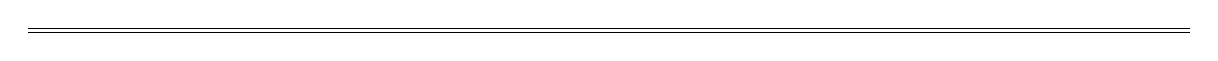
\begin{tikzpicture}%
		\draw (0, 0) -- (14.75, 0);%
		\draw (0, 0.05) -- (14.75, 0.05);%
	\end{tikzpicture}%
%\end{center}
}

\usepackage[
	hyperref = true,      	% Link to online documents
  	backend  = bibtex,      % Use bibtex instead of biber
  	sorting  = nyt,       	% Sorts by (name, year, title)
  	style  = alphabetic 	% Citations look like [Har77]
]{biblatex}
\addbibresource{SLP.bib}

\usepackage{geometry}
 \geometry{
 a4paper,
 % total={170mm,257mm},
 % left=20mm,
 bottom=20mm,
 }
\newenvironment{blockquote}
{\begin{mdframed}[skipabove=0pt, skipbelow=0pt, innertopmargin=4pt, innerbottommargin=4pt, bottomline=false,topline=false,rightline=false, linewidth=2pt]}
{\end{mdframed}}
\newenvironment{soln}{\begin{proof}[Solution]}{\end{proof}}

\def\univname{}
\def\coursenum{}
\def\coursename{Algebraic Topology}
\def\professor{Rekha Santhanam}
\def\student{Aryaman Maithani}
\def\semesteryear{Autumn 2020}
\def\imagename{iitb.png}		    % Replace with University Seal
\def\scalesize{0.20}					% Scale Logo Size 

% Style Package (Load After Cover Information)
\usepackage{style2}	% Change to match style file

\begin{document}
% \fontdimen2\font=1ex
% \maketitle
% \mytoc
% \setcounter{section}{-1}
\coverpage

% Last Updated
\updated{\today}

% Table of Contents
\thispagestyle{empty}
\tableofcontents
\newpage
\pagestyle{fancy}
\setcounter{section}{-1}
\setcounter{page}{1}

\tikzset{lab dis/.store in=\LabDis,
  lab dis=0.4,
  ->-/.style args={at #1 with label #2}{decoration={
    markings,
    mark=at position #1 with {\arrow{>}; \node at (0,\LabDis) {#2};}},postaction={decorate}},
  ->>-/.style args={at #1 with label #2}{decoration={
    markings,
    mark=at position #1 with {\arrow{>}; \node at (0,-\LabDis) {#2};}},postaction={decorate}},
  -<-/.style args={at #1 with label #2}{decoration={
    markings,
    mark=at position #1 with {\arrow{<}; \node at (0,\LabDis)
    {#2};}},postaction={decorate}},
  -<<-/.style args={at #1 with label #2}{decoration={
    markings,
    mark=at position #1 with {\arrow{<}; \node at (0,-\LabDis)
    {#2};}},postaction={decorate}},
  -*-/.style args={at #1 with label #2}{decoration={
    markings,
    mark=at position #1 with {{\fill (0,0) circle (1.5pt);} \node at (0,\LabDis)
    {#2};}},postaction={decorate}},
  -^-/.style args={at #1 with label #2}{decoration={
    markings,
    mark=at position #1 with {{\fill (0,0) circle (1.5pt);} \node at (0,-\LabDis)
    {#2};}},postaction={decorate}},
% 
   % -*-/.style={decoration={
   %  markings,
   %  mark=at position #1 with {\fill (0,0) circle (1.5pt);}},postaction={decorate}},
  }
\section{Preliminaries}
In what follows, $I$ will denote the closed interval $[0, 1] \subset \mathbb{R}.$\\
Whenever we talk about a map $f:X\to Y$ between topological spaces $X$ and $Y,$ we will always mean a \emph{continuous function} $f.$\\
A path $\sigma$ in a space $X$ is a map $\sigma: I \to X.$ If $x_0 = \sigma(0)$ and $x_1 = \sigma(1),$ we write this as
\begin{equation*} 
	x_0 \overset{\sigma}{\longrightarrow} x_1.
\end{equation*}
Moreover, $x_0$ and $x_1$ are called the \emph{end points} of $\sigma.$ In particular, $x_0$ is the initial point and $x_1$ is the terminal point.\\
All the topological spaces are assumed to be nonempty.

We now recall some basic theorems.

\begin{thm}[Pasting lemma] \label{thm:pastinglemma}
	Let $f:X\to Y$ be a function (not a priori continuous). Let $X_1, \ldots, X_n \subset X$ be closed sets such that
	\begin{equation*} 
		X = \bigcup_{i = 1}^n X_i.
	\end{equation*}
	If $f|_{X_i}$ is continuous for each $i,$ then $f$ is continuous.
\end{thm}

\begin{thm}[Union of connected sets]
	Let $X$ be a topological space and $\{A_\alpha\}$ be a collection of connected subsets of $X.$ If $\bigcap A_\alpha$ is nonempty, then $\bigcup A_\alpha$ is connected.
\end{thm}

\begin{thm}[Lebesgue Number Lemma] \label{thm:lebesgue}
	Let $\sigma:I\to X$ be a path. Let $\{A_\alpha\}$ be an open cover of $X.$ Then, there exists a finite partition
	\begin{equation*} 
		0 = t_0 < t_1 < \cdots < t_n = 1
	\end{equation*}
	such that for each $i = 1, \ldots, n,$ the image $\sigma([t_{i - 1}, t_i])$ in contained in some $A_{\alpha_i}.$
\end{thm}
The above can also be modified for a function $f:I^2 \to X$ where we partition $I^2$ into smaller rectangles.

\begin{thm}[The Eckmann-Hilton Argument] \label{thm:eckmannhilton}
	Let $M$ be a set and $*, \star$ be two unital binary operations on $M$ with units $1_*$ and $1_\star,$ respectively. Suppose that
	\begin{equation*} 
		(a * b) \star (c * d) = (a \star c) * (b \star d)
	\end{equation*}
	for all $a, b, c, d \in M.$\\
	Then, $1_* = 1_\star,$ $* = \star,$ and furthermore, the operation(s) are commutative and associative.
\end{thm}
\begin{proof} \phantom{hi}\\
	\textbf{Claim 1.} $1_* = 1_\star.$
	\begin{align*} 
		1_* = 1_* * 1_* &= (1_* \star 1_\star) * (1_\star \star 1_*)\\
		&=(1_* * 1_\star) \star (1_\star * 1_*) = 1_\star \star 1_\star = 1_\star.
	\end{align*}
	Thus, we define $1 \vcentcolon= 1_* = 1_\star$ which is the unit for both operations.

	\myfilll

	\textbf{Claim 2.} $a*b = a\star b$ for all $a, b \in M.$
	\begin{align*} 
		a * b &= (a \star 1) * (1 \star b)\\
		&= (a * 1) \star (1 * b) = a \star b.
	\end{align*}
	Thus, we define $\cdot = * = \star.$

	\myfilll

	\textbf{Claim 3.} $a\cdot b = b\cdot a$ for all $a, b \in M.$
	\begin{align*} 
		a \cdot b &= (1 \cdot a) \cdot (b \cdot 1)\\
		&= (1 \cdot b) \cdot (a \cdot 1) = b \cdot a.
	\end{align*}

	\myfilll

	\textbf{Claim 4.} $(a\cdot b) \cdot c = a\cdot(b\cdot c)$ for all $a, b, c \in M.$
	\begin{align*} 
		(a\cdot b) \cdot c &= (a\cdot b) \cdot (1 \cdot c)\\
		&= (a\cdot 1) \cdot (b \cdot c) = a \cdot (b \cdot c).
	\end{align*}

	Thus, we have proven all the claims.
\end{proof}
\section{Homotopy of Paths}
%
\subsection{The Fundamental Group}

\begin{defn}[Homotopy]
	Let $\sigma$ and $\tau$ be paths in a space $X$ with the same end points, i.e., $\sigma(0) = \tau(0)$ and $\sigma(1) = \tau(1).$\\
	We say that $\sigma$ and $\tau$ are \emph{homotopic with ends points held fixed} written
	\begin{equation*} 
		\sigma \simeq \tau \rel \{0, 1\}
	\end{equation*}
	if there is a map $F: I \times I \to X$ such that
	\begin{enumerate}
		\item $F(s, 0) = \sigma(s)$ for all $s \in I,$
		\item $F(s, 1) = \tau(s)$ for all $s \in I,$
		\item $F(0, t) = x_0$ for all $t \in I,$
		\item $F(1, t) = x_1$ for all $t \in I.$
	\end{enumerate}
	$F$ is called a \emph{homotopy} from $\sigma$ to $\tau.$ We write
	\begin{equation*} 
		F : \sigma \simeq \tau \rel \{0, 1\}.
	\end{equation*}
\end{defn}
The above can be pictorially depicted as

\begin{center}
	\begin{tikzpicture}
		\def \len{2.5}
		\draw[thick, ->-=at 0.5 with label {$x_0$}](0, 0) -- (0, \len);
		\draw[thick, ->-=at 0.5 with label {$\tau$}](0, \len) -- (\len, \len);
		\draw[thick, -<-=at 0.5 with label {$x_1$}](\len, \len) -- (\len, 0);
		\draw[thick, -<-=at 0.5 with label {$\sigma$}](\len, 0) -- (0, 0);
	\end{tikzpicture}
\end{center}

The above picture is interpreted as follows: \\
Along the (bottom) line $t = 0,$ $F$ agrees with $\sigma$ and along the (top) line $t = 1,$ $F$ agrees with $\tau.$\\
Similarly, along the (left) line $s = 0,$ $F$ is identically equal to $x_0$ and along the (right) line $s = 1,$ it is $x_1.$

%
In particular, if $\sigma$ is a \emph{loop}, i.e., $x_0 = x_1$ and $e_{x_0}$ is the constant loop $s \mapsto x_0$ for $s \in I,$ and if $\sigma \simeq e_{x_0} \rel \{0, 1\},$ we say that ``$\sigma$ can be shrunk to a point,'' or is \emph{homotopically trivial}.

\begin{prop}[$\simeq$ is an equivalence relation] \label{prop:equivrel}
	\begin{enumerate}
		\item $\sigma \simeq \sigma \rel \{0, 1\},$
		\item $\sigma \simeq \tau \rel \{0, 1\} \implies \tau \simeq \sigma \rel \{0, 1\},$
		\item $\sigma \simeq \tau \rel \{0, 1\}$ and $\tau \simeq \rho \rel \{0, 1\} \implies \sigma \simeq \rho \rel \{0, 1\}.$ 
	\end{enumerate}
\end{prop}
\begin{proof} 
	\begin{enumerate}
		\item Define $F(s, t) \vcentcolon= \sigma(s).$
		\item Define $F(s, t) \vcentcolon= F(s, 1 - t).$
		\item Given $F:\sigma \simeq \tau \rel \{0, 1\}$ and $G:\tau \simeq \rho \rel \{0, 1\},$ define $H:I \times I \to X$ as

		\begin{equation*} 
			H(s, t) \vcentcolon= \begin{cases}
				F(s, 2t) & 0 \le 2t \le 1,\\
				G(s, 2t - 1) & 1 \le 2t \le 2.
			\end{cases}
		\end{equation*}
		Note that $F$ and $G$ do agree for $2t = 1$ since we have $F(s, 1) = \tau(s) = G(s, 0)$ for all $s \in I.$ It is easy to see that $H$ is well-defined.\\
		Note that $H$ is continuous (by the \nameref{thm:pastinglemma}) and it satisfies all the four properties of a homotopy (from $\sigma$ to $\rho$), since $F$ and $G$ do so. \qedhere
	\end{enumerate}
\end{proof}
Thus, we can consider the homotopy classes $[\sigma]$ of paths $\sigma$ from $x_0$ to $x_1$ under the equivalence relation $\simeq.$ (Note very carefully that all paths in an equivalence class have the same end points.)

\begin{defn}[Multiplication of paths]
	Let $\sigma$ be a path from $x_0$ to $x_1$ and $\tau$ from $x_1$ to $x_2.$\\
	The product $\sigma*\tau$ is a path from $x_0$ to $x_2$ defined as
	\begin{equation*} 
		\sigma*\tau(s) \vcentcolon= \begin{cases}
			\sigma(2s) & 0 \le 2s \le 1,\\
			\tau(2s - 1) & 1 \le 2s \le 2.
		\end{cases}
	\end{equation*}
	Once again, it's an easy check that $\sigma\tau$ is well-defined and continuous (using the \nameref{thm:pastinglemma}).
\end{defn}

The above $\sigma*\tau$ is essentially the path from $x_0$ to $x_1$ obtained by first travelling from $x_0$ to $x_1$ via $\sigma$ and then from $x_1$ to $x_2$ via $\tau.$

We will now be lenient with notation and simply denote $\sigma*\tau$ as $\sigma\tau$ unless otherwise necessary.\\
The next proposition shows how this product behaves with the equivalence relation.

\begin{prop}
	\begin{equation*} 
		\sigma \simeq \sigma' \rel \{0, 1\} \text{ and } \tau \simeq \tau' \rel \{0, 1\} \implies \sigma\tau \simeq \sigma'\tau' \rel \{0, 1\}.
	\end{equation*}
\end{prop}
\begin{proof} 
	The proof is motivated by the following diagram.
	
	\begin{center}	\begin{tikzpicture}
			\def \len{3}
			\draw[thick, ->-=at 0.5 with label {$x_0$}](0, 0) -- (0, \len);
			\draw[thick, ->-=at 0.5 with label {$\sigma'$}](0, \len) -- (\len, \len);
			\draw[dashed, -<-=at 0.5 with label {$x_1$}, -*-=at 0.0 with label {}, -*-=at 1.0 with label {}](\len, \len) -- (\len, 0);
			\draw[thick, -<-=at 0.5 with label {$\sigma$}](\len, 0) -- (0, 0);
			\draw[thick, ->-=at 0.5 with label {$\tau'$}](\len, \len) -- (2*\len, \len);
			\draw[thick, -<-=at 0.5 with label {$x_2$}](2*\len, \len) -- (2*\len, 0);
			\draw[thick, -<-=at 0.5 with label {$\tau$}](2*\len, 0) -- (\len, 0);
			\node[] at (\len/2, \len/2) {$F$};
			\node[] at (3*\len/2, \len/2) {$G$};
		\end{tikzpicture}
	\end{center}

	Given $F:\sigma \simeq \sigma' \rel \{0, 1\}$ and $G:\tau \simeq \tau' \rel \{0, 1\},$ define $H:I \times I \to X$ as

	\begin{equation*} 
		H(s, t)\vcentcolon= \begin{cases}
				F(2s, t) & 0 \le 2s \le 1,\\
				G(2s - 1, t) & 1 \le 2s \le 2.
			\end{cases}
	\end{equation*}

	As earlier, $H$ is well-defined (since $F(1, t) = x_1 = G(0, t)$ for all $t \in I$) and continuous. Moreover, we have
	\begin{equation*} 
		H(0, t) = F(0, t) = x_0, \quad H(1, t) = G(1, t) = x_2,
	\end{equation*}
	\begin{equation*} 
		H(s, 0)= \begin{cases}
				F(2s, 0) & 0 \le 2s \le 1,\\
				G(2s - 1, 0) & 1 \le 2s \le 2
			\end{cases} = \begin{cases}
				\sigma(2s) & 0 \le 2s \le 1,\\
				\tau(2s - 1) & 1 \le 2s \le 2
			\end{cases} = \sigma\tau(s),
	\end{equation*}
	and similarly, 
	\begin{equation*} 
		H(s, 1) = \sigma'\tau'(s)\text{ for all }s \in I.
	\end{equation*}\\
	This shows that 
	\begin{equation*} 
		H : \sigma\tau\simeq\sigma'\tau' \rel \{0, 1\}. \qedhere
	\end{equation*}
\end{proof}
\begin{defn}[Product of equivalence classes]
	In view of the above proposition, we define
	\begin{equation*} 
		[\sigma]*[\tau] \vcentcolon= [\sigma*\tau].
	\end{equation*}
\end{defn}
The above, of course, is defined only when the terminal point of $\sigma$ (and thus, any other representative of $[\sigma]$) equals the initial point of $\tau$ (and thus, any other representative of $[\tau]$).\\
As before, we shall drop the $*$ and simply write $[\sigma][\tau].$

\begin{lem} \label{lem:prodassoc}
	Let $\sigma, \tau, \omega$ be paths such that the products $\sigma(\tau\omega)$ and $(\sigma\tau)\omega$ are defined. Then,
	\begin{equation*} 
		\sigma(\tau\omega) \simeq (\sigma\tau)\omega \rel \{0, 1\}.
	\end{equation*}
\end{lem}
It is clear that $\sigma(\tau\omega)$ is defined iff $(\sigma\tau)\omega$ is.
\begin{proof} 
	Let $x_0, x_1, x_2, x_3$ be points such that
	\begin{equation*} 
		x_0 \overset{\sigma}{\longrightarrow} x_1 \overset{\tau}{\longrightarrow} x_2 \overset{\omega}{\longrightarrow} x_3. 
	\end{equation*}
	We define a homotopy $F$ from $\sigma(\tau\omega)$ to $(\sigma\tau)\omega.$ To motivate the definition of $F,$ we may first visualise the homotopy as follows.
	\begin{center}
		\begin{tikzpicture}
			\def\len{2}
			\def\height{3}
	\draw[thick, ->-=at 0.5 with label {$x_0$}](0, 0) -- (0, \height);
	\draw[thick, ->-=at 0.5 with label {$\sigma$}](0, \height) -- (\len, \height);
	\draw[thick, ->-=at 0.5 with label {$\tau$}](\len, \height) -- (2*\len, \height);
	\draw[thick, ->-=at 0.5 with label {$\omega$}](2*\len, \height) -- (4*\len, \height);
	\draw[thick, -<-=at 0.5 with label {$x_3$}](4*\len, \height) -- (4*\len, 0);
	\draw[thick, -<-=at 0.5 with label {$\omega$}](4*\len, 0) -- (3*\len, 0);
	\draw[thick, -<-=at 0.5 with label {$\tau$}](3*\len, 0) -- (2*\len, 0);
	\draw[thick, -<-=at 0.5 with label {$\sigma$}](2*\len, 0) -- (0, 0);
	\draw[dashed,-*-=at 0.0 with label {},-*-=at 1.0 with label {}](\len, \height) -- (2*\len, 0);
	\draw[dashed, -*-=at 0.0 with label {}, -*-=at 1.0 with label {}](2*\len, \height) -- (3*\len, 0);
		\end{tikzpicture}
	\end{center}
	One can note that the top line depicts the path $(\sigma\tau)\omega$ and the bottom $\sigma(\tau\omega).$

	We define $F:I \times I \to X$ piece-wise on the three regions (from left to right) as follows:

	\begin{equation*} 
		F(s, t) \vcentcolon= \begin{cases}
			\sigma\left(\dfrac{4s}{2 - t}\right) & 0 \le s \le \dfrac{1}{4}(2 - t) ,\\~\\	\tau\left(4s + 2 - t\right) & \dfrac{1}{4}(2 - t) \le s \le \dfrac{1}{4}(3 - t),\\~\\
        	\omega\left(\dfrac{4s + t - 3}{t + 1}\right) & \dfrac{1}{4}(3 - t) \le s \le 1.
		\end{cases}
	\end{equation*}
	It is clear that $F$ is continuous on each piece. By the \nameref{thm:pastinglemma}, it is continuous everywhere.\\
	The four properties of being a homotopy are also clear, by construction. (The diagram makes it clear why.)
\end{proof}

\begin{defn}[Inverse path]
	Given a path $\sigma$ from $x_0$ to $x_1,$ its \emph{inverse path} $\sigma^{-1}$ is a path from $x_1$ to $x_0$ given by
	\begin{equation*} 
		\sigma^{-1}(s) \vcentcolon= \sigma(1 - s), \qquad s \in I.
	\end{equation*}
\end{defn}
The above is simply ``travelling backwards $\sigma$.''
\begin{lem} 
	Let $\sigma, \sigma':I \to X$ be paths such that $\sigma \simeq \sigma' \rel \{0, 1\}.$ Then,
	\begin{equation*} 
		\sigma^{-1} \simeq \sigma'^{-1} \rel \{0, 1\}.
	\end{equation*}
\end{lem}
\begin{proof} 
	Let $F:\sigma \simeq \sigma' \rel \{0, 1\}$ be a homotopy. Then, $F'(s, t) \vcentcolon= F(1 - s, t)$ is a homotopy between the inverses.
\end{proof}

\begin{defn}[Inverse class]
	Let $\sigma:I \to X$ be a path. We define the inverse of the class $[\sigma]$ as
	\begin{equation*} 
		[\sigma]^{-1} \vcentcolon= [\sigma^{-1}].
	\end{equation*}
\end{defn}
In view of the above lemma, the above definition is indeed well-defined.

\begin{lem} \label{lem:prodinv}
	Given any path $\sigma$ from $x_0$ to $x_1,$ we have
	\begin{equation*} 
		e_{x_0} \simeq \sigma\sigma^{-1} \rel \{0, 1\},
	\end{equation*}
	where $e_{x_0}$ denotes the constant loop at $x_0.$
\end{lem}

\begin{proof} 
	As usual, we motivate the proof with a diagram. In this case, it is the following:
	\begin{center}
		\begin{tikzpicture}
			\def\len{3}
			\draw[thick, ->-=at 0.5 with label {$x_0$}](0, 0) -- (0, \len);
			\draw[thick, ->-=at 0.5 with label {$\sigma$}](0, \len) -- (\len, \len);
			\draw[thick, -<-=at 0.5 with label {$e_{x_0}$}](2*\len, 0) -- (0, 0);
			\draw[thick, ->-=at 0.5 with label {$\sigma^{-1}$}](\len, \len) -- (2*\len, \len);
			\draw[thick, -<-=at 0.5 with label {$x_0$}](2*\len, \len) -- (2*\len, 0);
			\draw[dashed, -*-=at 0.5 with label {$x_1$}] (0, 0) -- (\len, \len) -- (2*\len, 0);
		\end{tikzpicture}
	\end{center}
	The homotopy $F:I \times I \to X$ in this case, is defined as
	\begin{equation*} 
		F(s, t) \vcentcolon= \begin{cases}
			\sigma(2s) & 0 \le 2s \le t,\\
			\sigma(t) & t \le 2s \le 2 - t,\\
			\sigma^{-1}(2s - 1) & 2 - t \le 2s \le 2.
		\end{cases}
	\end{equation*}
	It is clear that the piecewise definitions agree on the dashed line $2s = t.$ Observe that $\sigma^{-1}(2s - 1) = \sigma(2 - 2s)$ and thus, the functions do agree on the dashed line $2s = 2 - t$ as well. \\
	One can easily check that the four properties of the homotopy are satisfied. To see the bottom line property, note that $F(s, 0) = \sigma(0)$ (using the second piece definition) and $\sigma(0) = x_0 = e_{x_0}(s)$ for all $s \in I.$
\end{proof}

Note that since $(\sigma^{-1})^{-1} = \sigma,$ the above also shows that $\sigma^{-1}\sigma = e_{x_1}.$

\begin{lem} \label{lem:leftid}
	Let $x_0 \overset{\sigma}{\longrightarrow} x_1$ and $e_{x_0}$ be the constant path at $x_0.$ Then,
	\begin{equation*} 
		\sigma \simeq e_{x_0}\sigma \rel \{0, 1\}.
	\end{equation*}
\end{lem}
\begin{proof} 
	The proof is motivated by this diagram.

	\begin{center}
		\begin{tikzpicture}
			\def\len{3}
			\draw[thick, ->-=at 0.5 with label {$x_0$}](0, 0) -- (0, \len);
			\draw[thick, ->-=at 0.5 with label {$e_{x_0}$}](0, \len) -- (\len, \len);
			\draw[thick, -<-=at 0.5 with label {$\sigma$}](2*\len, 0) -- (0, 0);
			\draw[thick, ->-=at 0.5 with label {$\sigma$}](\len, \len) -- (2*\len, \len);
			\draw[thick, -<-=at 0.5 with label {$x_1$}](2*\len, \len) -- (2*\len, 0);
			\draw[dashed, -*-=at 1.0 with label {$x_0$}] (0, 0) -- (\len, \len);
		\end{tikzpicture}
	\end{center}

	The homotopy is $F:I\times I \to X$ defined as
	\begin{equation*} 
		F(s, t) \vcentcolon= \begin{cases}
			x_0 & 0 \le 2s \le t,\\~\\
    	\sigma\left(\dfrac{2s - t}{2 - t}\right) & t \le 2s \le 2.
		\end{cases}
		\qedhere
	\end{equation*}
\end{proof}

As one would expect, we have a lemma in the other direction as well.
\begin{lem} \label{lem:rightid}
	Let $x_1 \overset{\sigma}{\longrightarrow} x_0$ and $e_{x_0}$ be the constant path at $x_0.$ Then,
	\begin{equation*} 
		\sigma \simeq \sigma e_{x_0} \rel \{0, 1\}.
	\end{equation*}
\end{lem}

\begin{proof} 
	Similar as in the last case and we omit it.
\end{proof}
	
The astute reader might have sensed a group sneaking around the corner.\\
However, note that the product of equivalence classes defined above is not a binary operation unless the endpoints are the same. Due to this, we restrict ourselves to loops in the next theorem.

\begin{thm}
	Let $\pi_1(X, x_0)$ be the set of homotopy classes of loops in $X$ at $x_0.$\\
	If multiplication in $\pi_1(X, x_0)$ is defined as above, $\pi_1(X, x_0)$ becomes a group, in which the neutral element is the class $[e_{x_0}]$ and the inverse of a class $[\sigma]$ is the class of the inverse $[\sigma^{-1}].$
\end{thm}
\begin{proof} 
	Interpreting \crefrange{lem:prodassoc}{lem:rightid} as equalities of the equivalence classes shows that $\pi_1(X, x_0)$ verifies the group axioms.
\end{proof}

The next proposition tells us how $\pi_1(X, x_0)$ and $\pi_1(X, x_1)$ are related in the case that $x_0$ and $x_1$ lie in the same path-connected component. (In the case that they do not, nothing can be said.)

\begin{prop} \label{prop:alphainducesiso1}
	Let $\alpha$ be a path from $x_0$ to $x_1.$ The mapping $\widehat{\alpha}$ defined by
	\begin{equation*} 
		[\sigma] \mapsto [\alpha^{-1}]*[\sigma]*[\alpha] = [\alpha^{-1}\sigma\alpha]
	\end{equation*}
	is an isomorphism of the group $\pi_1(X, x_0)$ onto $\pi_1(X, x_1).$
\end{prop}
Note that the above is well-defined since $*$ is well-defined.
\begin{proof} 
	We first note that if $[\sigma] \in \pi_1(X, x_0),$ then $\alpha^{-1}\sigma\alpha$ is path as follows:
	\begin{equation*} 
		x_1 \overset{\alpha^{-1}}{\longrightarrow} x_0 \overset{\sigma}{\longrightarrow} x_0 \overset{\alpha}{\longrightarrow} x_1
	\end{equation*}
	and thus, $[\alpha^{-1}\sigma\alpha]$ is indeed an element of $\pi_1(X, x_1).$\\
	Moreover, note that
	\begin{align*} 
		\widehat{\alpha}([\sigma\sigma']) &= [\alpha^{-1}\sigma\sigma'\alpha]\\
		&= [\alpha^{-1}\sigma][\sigma'\alpha]\\
		&= [\alpha^{-1}\sigma][\alpha\alpha^{-1}][\sigma'\alpha]\\
		&= [\alpha^{-1}\sigma\alpha][\alpha^{-1}\sigma'\alpha]\\
		&= \widehat{\alpha}([\sigma])\widehat{\alpha}([\sigma']).
	\end{align*}
	This shows that $\widehat{\alpha}$ is a homomorphism. That this is an isomorphism follows by noting that it has as inverse $\widehat{\alpha^{-1}}.$
\end{proof}
\begin{cor}
	If $X$ is path-connected, the group $\pi_1(X, x_0)$ is independent of the point $x_0,$ up to isomorphism.
\end{cor}
Note that if $C$ is a connected component of $X$ containing $x_0,$ then $\pi_1(X, x_0) = \pi_1(C, x_0)$ since any loop at $x_0$ must necessarily lie in $C.$ For this reason, we might as well only work with path-connected spaces.
\begin{defn}
	If $X$ is path-connected, we write $\pi_1(X)$ for $\pi_1(X, x_0)$ and call it \emph{the fundamental group} of $X.$
\end{defn}
Note that this group depends on $x_0$ in the sense that the elements of the group depend on the base point $x_0$ but the isomorphism class does not.\\
\begin{defn}[Simply connected]
	A space $X$ is called simply connected if it is path-connected and its fundamental group is trivial.
\end{defn}
\begin{lem} \label{lem:simpconnpathshomot}
	Let $X$ be simply connected. If $\sigma$ and $\tau$ are paths in $X$ with the same initial and terminal points, then $\sigma \simeq \tau \rel \{0, 1\}.$
\end{lem}
\begin{proof} 
	Let the initial and terminal points be $x_0$ and $x_1,$ respectively.\\
	Consider the path $\sigma\tau^{-1},$ which is path at $x_0.$ Since $X$ is simply connected, we have
	\begin{equation*} 
		\sigma\tau^{-1} \simeq e_{x_0} \rel \{0, 1\}.
	\end{equation*}
	By the previously seen properties, we see that
	\begin{equation*} 
		(\sigma\tau^{-1})\tau \simeq e_{x_0}\tau \rel \{0, 1\}
	\end{equation*}
	or
	\begin{equation*} 
		\sigma \simeq \tau \rel \{0, 1\}. \qedhere
	\end{equation*}
\end{proof}
\subsection{Functoriality} \label{subsec:functor}
We now wish to turn $\pi_1$ into a functor. Since we need to take care of the base points, we look at the category of \emph{Pointed Topological spaces}.
\begin{defn}[Pointed Topological Spaces]
	The category $\mathsf{Top}_\bullet$ of \emph{pointed topological spaces} is the category whose objects and morphisms are given as follows:
	\begin{itemize}
		\item Objects: Pairs $(X, x_0)$ where $X$ is a topological space and $x_0 \in X,$
		\item Morphisms: $f:(X, x_0) \to (Y, y_0)$ such that $f:X\to Y$ is a continuous function and $f(x_0) = y_0.$
	\end{itemize}
\end{defn}
That the above is a category can be easily verified.

\begin{defn}
	Let $h:(X, x_0) \to (Y, y_0)$ be a morphism. Define
	\begin{equation*} 
		h_* : \pi_1(X, x_0) \to \pi_1(Y, y_0)
	\end{equation*}
	by the equation
	\begin{equation*} 
		h_*([\sigma]) = [h\circ \sigma].
	\end{equation*}
	The map $h_*$ is called the \emph{homomorphism induced by $h$}, relative to the base point $x_0.$
\end{defn}
To see that $h_*$ is well-defined, we note that if 
\begin{equation*} 
	F : \sigma \simeq \sigma' \rel \{0, 1\}
\end{equation*}
for loops $\sigma, \sigma'$ in $X$ at $x_0,$ then
\begin{equation*} 
	h \circ F : h\circ \sigma \simeq h\circ\sigma' \rel \{0, 1\}.
\end{equation*}
That is to say, if two loops at $x_0$ are homotopic, then so are the loops obtained by pre-composing $h.$

To see that $h_*$ is a homomorphism, first note that
\begin{equation*} 
	(h \circ \sigma)(h \circ \sigma') = h\circ(\sigma\sigma').
\end{equation*}
(This follows from the definition of the product of paths.)\\
Then, we see that
\begin{equation*} 
	h_*([\sigma\sigma']) = [h\circ(\sigma\sigma')] = [h\circ\sigma][h\circ\sigma'] = h_*([\sigma])h_*([\sigma']).
\end{equation*}

\begin{thm}[Functoriality]
	If $h:(X, x_0) \to (Y, y_0)$ and $k:(Y, y_0) \to (Z, z_0)$ are morphisms, then
	\begin{equation*} 
		(k \circ h)_* = k_* \circ h_*.
	\end{equation*}
	If $i:(X, x_0) \to (X, x_0)$ is the identity map, then $i_*$ is the identity homomorphism.
\end{thm}
\begin{proof} 
	By definition, we have
	\begin{align*} 
		(k \circ h)_*([\sigma]) &= [(k \circ h) \circ \sigma]\\
		&= [k \circ (h \circ \sigma)]\\
		&= k_*([h\circ \sigma])\\
		&= k_*(h_*([\sigma]))\\
		&= (k_* \circ h_*)([\sigma]).
	\end{align*}
	Thus, $(k \circ h)_* = k_* \circ h_*.$

	Now, if $i$ is the identity map, then we have
	\begin{equation*} 
		i_*([\sigma]) = [i \circ \sigma] = [\sigma],
	\end{equation*}
	showing that $i_*$ is the identity map of $\pi_1(X, x_0).$
\end{proof}
The above then shows that $\pi_1$ defines a functor from the category $\mathsf{Top}_*$ to $\mathsf{Grp}.$\\
Since functors preserve isomorphisms in general, we get the following corollary.
\begin{cor}
	If $h:(X, x_0) \to (Y, y_0)$ is a morphism such that $h:X \to Y$ is a homeomorphism, then
	\begin{equation*} 
		h_* : \pi_1(X, x_0) \to \pi_1(Y, y_0)
	\end{equation*}
	is an isomorphism.
\end{cor}
Since we aren't discussing Category Theory, we give a proof for this special example of functors.
\begin{proof} 
	Let $h^{-1}:Y \to X$ be the inverse, which is continuous since $h$ is a homeomorphism. Moreover, $h^{-1}(y_0) = x_0$ and thus, $h^{-1}:(Y, y_0) \to (X, x_0)$ is a morphism and the inverse of $h.$\\
	Now, note that,
	\begin{equation*} 
		(h_*)\circ((h^{-1})^*) = (h\circ h^{-1})^* = (\id_{(Y, y_0)})^* = \id_{\pi_1(Y, y_0)},
	\end{equation*}
	by functoriality. Similarly, we have
	\begin{equation*} 
		((h^{-1})^*)\circ(h_*) = \id_{(X, x_0)},
	\end{equation*}
	proving the corollary.
\end{proof}
%
%
\section{Homotopy of Maps}
%
In the previous section, we talked about homotopy of special types of maps. More precisely, we only considered maps $I \to X.$ However, we can replace $I$ by an arbitrary topological space $Y.$ In the place of endpoints, we just consider a subspace $A \subset Y.$
\begin{defn}[Relative homotopy]
	Given maps $f, g:Y \to X$ such that $f|_A = g|_A,$ we say $f$ and $g$ are homotopic relative to $A$ written
	\begin{equation*} 
		f \simeq g \rel A
	\end{equation*}
	if there is a map $F:Y \times I \to X$ satisfying
	\begin{enumerate}
		\item $F(y, 0) = f(y)$ for all $y \in Y,$
		\item $F(y, 1) = g(y)$ for all $y \in Y,$
		\item $F(a, t) = f(a) = g(a)$ for all $a \in A, t \in I.$
	\end{enumerate}
	This map $F$ is called a homotopy from $f$ to $g$ relative to $A$ and we write
	\begin{equation*} 
		F:f\simeq g \rel A.
	\end{equation*}
\end{defn}
Note that the ``second coordinate'' above is still $I.$\\
Note that (3) is satisfied vacuously if $A = \emptyset$ and we have $f|_A = g|_A$ for all maps $f, g : Y \to X.$ Keeping this in mind, we have the following definition.
\begin{defn}[Homotopy]
	Maps $f, g:Y \to X$ are said to be \emph{homotopic} if $f$ and $g$ are homotopic relative to $\emptyset.$\\
	We write this more simply as
	\begin{equation*} 
		f \simeq g.
	\end{equation*}
	Moreover, any $F$ as before is simply called a homotopy from $f$ to $g.$\\
	As before, we write
	\begin{equation*} 
		F:f\simeq g.
	\end{equation*}
\end{defn}

Once again, we obtain an equivalence. The homotopies defined as in the proof of \cref{prop:equivrel} work again.
\begin{defn}[Contractible space] \label{def:contrac}
	If $X$ is a topological space such that the identity map on $X$ is homotopic to a constant map on some point in $X,$ we say that $X$ is \emph{contractible}.
\end{defn}

\begin{prop} \label{prop:contracpath} % ex 3.1
	$X$ is contractible if and only if for any space $Y,$ any two maps of $Y$ into $X$ are homotopic. A contractible space is path-connected.
\end{prop}
\begin{proof} 
	$(\implies)$ Let $X$ be contractible and $Y$ be any space. Fix any $x_0 \in X$ such that $\id_X$ is homotopic to the constant map $e_{x_0}:X\to X.$ \\
	Let $f_{x_0}:Y\to X$ denote the constant map $y \mapsto x_0.$\\
	Now, given any map $f:Y\to X,$ we show that it is homotopic to $f_{x_0}.$ \\This will prove that any two maps of $Y$ into $X$ are homotopic since $\simeq$ is an equivalence relation.\\
	Let $H:\id_X \simeq e_{x_0}$ be any homotopy. Then, we have
	\begin{equation*} 
		H(x, 0) = x,\quad H(x, 1) = x_0; \qquad \text{for all } x \in X.
	\end{equation*}
	(Note that $H$ is continuous.)\\
	Now, we define $F:Y\times I \to X$ as
	\begin{equation*} 
		F(y, t) = H(f(y), t).
	\end{equation*}
	It is clear that $F$ is a map. (That is, $F$ is continuous.)\\
	Moreover, note that
	\begin{equation*} 
		F(y, 0) = H(f(y), 0) = f(y), \quad F(y, 1) = H(f(y), 1) = x_0 = f_{x_0}(y); \qquad \text{for all } y \in Y.
	\end{equation*}
	This shows that $F:f\simeq f_{x_0},$ as desired.

	$(\impliedby)$ To show that $X$ is contractible, simply consider $Y = X$ and consider the maps $\id_X$ and $e_{x_0}.$ (Both of these are indeed continuous.)\\
	By hypothesis, these maps are homotopic and by definition, $X$ is contractible.

	Now, we show that $X$ is path-connected assuming that it is contractible.\\
	Let $x_0$ and $x_1$ be any two points in $X.$ As $X$ is contractible, $(\implies)$ tells us that the maps $e_{x_0}$ and $e_{x_1}$ are homotopic. \\
	Let $F$ be any homotopy from $e_{x_0}$ and $e_{x_1}.$ Define $\sigma:I\to X$ as 
	\begin{equation*} 
		\sigma(t) \vcentcolon= F(x_0, t).
	\end{equation*}
	$\sigma$ is clearly continuous. Moreover, we have
	\begin{align*} 
		\sigma(0) &= F(x_0, 0) = e_{x_0}(x_0) = x_0,\\
		\sigma(1) &= F(x_0, 1) = e_{x_1}(x_0) = x_1.
	\end{align*}
	Thus, $\sigma$ is path from $x_0$ to $x_1$ in $X,$ proving the proposition.
\end{proof}
\begin{ex}
	Every convex subset $X$ of Euclidean space is contractible.

	\myfill

	Given maps $f_1, f_2: Y \to X,$ we have a homotopy $F:f_1 \simeq f_2$ given by
	\begin{equation*} 
		F(y, t) = tf_2(y) + (1 - t)f_1(y), \quad y \in Y, t \in I.
	\end{equation*}
	By the convexity assumption, the above $F$ is indeed a map into $X.$\\
	By the previous proposition, this shows that $X$ is contractible.
\end{ex}
\begin{ex}
	$\mathbb{R}^n$ is contractible for any $n.$

	\myfill

	To see this, we could either appeal to the previous example or do it directly by defining a homotopy $F: e_{0} \simeq \id_{\mathbb{R}^n}$ as
	\begin{equation*} 
		F(x, t) = tx.
	\end{equation*}
\end{ex}

We would now like to show that any contractible space is simply connected. What we do know is that any loop would be homotopic to a point. However, we do not know if this homotopy is relative to $\{0, 1\}.$ Indeed, to show that we do have a homotopy relative to $\{0, 1\},$ we would need to use the fact that $X$ is contractible once again.\\
Before proving that, we first look at a lemma.

\begin{lem} \label{lem:gbad}
	Let $F:I\times I \to X$ be a map. Set $\alpha(t) = F(0, t),$ $\beta(t) = F(1, t),$ $\gamma(s) = F(s, 0),$ and $\delta(s) = F(s, 1),$ as in the diagram
	\begin{center}
		\begin{tikzpicture}
			\def \len{3}
			\draw[thick, ->-=at 0.5 with label {$\alpha$}](0, 0) -- (0, \len);
			\draw[thick, ->-=at 0.5 with label {$\delta$}](0, \len) -- (\len, \len);
			\draw[thick, -<-=at 0.5 with label {$\beta$}](\len, \len) -- (\len, 0);
			\draw[thick, -<-=at 0.5 with label {$\gamma$}](\len, 0) -- (0, 0);
			\node[] at (\len/2, \len/2) {$F$};
		\end{tikzpicture}
	\end{center}
	Then, $\delta \simeq (\alpha^{-1}\gamma)\beta \rel \{0, 1\}.$
\end{lem}
\begin{proof} 
	The proof is quite intuitive. First, we define the paths
	\begin{equation*} 
		\sigma:I \to I\times I, \quad \tau:I \to I \times I
	\end{equation*}
	as
	\begin{equation*} 
		\sigma(s) \vcentcolon= (t, 1)
	\end{equation*}
	and
	\begin{equation*} 
		\tau(s) \vcentcolon= \begin{cases}
			(0, 1 - 4s) & 0 \le 4s \le 1, \\
			(4s - 1, 0) & 1 \le 4s \le 2, \\
			(1, 2s - 1) & 1 \le 2s \le 2.
		\end{cases}
	\end{equation*}
	These paths are the following ones in $I^2:$
	\begin{center}
		\begin{tikzpicture}
			\def \len{3}
			\draw[thick, ->-=at 0.5 with label {$\sigma$}](0, \len) -- (\len, \len);
			\draw[red, thick, -<-=at 0.5 with label {}](0, 0) -- (0, \len);
			\draw[red, thick, -<-=at 0.5 with label {}](\len, \len) -- (\len, 0);
			\draw[red, thick, -<-=at 0.5 with label {$\tau$}](\len, 0) -- (0, 0);
		\end{tikzpicture}
	\end{center}
	As it should be clear from the diagram (and one can easily check), we have
	\begin{equation*} 
		\delta = F \circ \sigma, \quad (\alpha^{-1}\gamma)\beta = F \circ \tau.
	\end{equation*}
	(Note that the bracketing in $(\alpha^{-1}\gamma)\beta$ is necessary.)\\
	Also, since $I^2$ is convex, we see that $\sigma$ and $\tau$ are homotopic relative to $\{0, 1\}$ with $H:I\times I \to I\times I$ being a required homotopy defined as
	\begin{equation*} 
		H(s , t) \vcentcolon= (1 - t)\sigma(s) + t\tau(s).
	\end{equation*}
	Thus,
	\begin{align*} 
		F \circ H &: F \circ \sigma \simeq F \circ \tau \rel \{0, 1\}\\
		\implies F \circ H &: \delta \simeq (\alpha^{-1}\gamma)\beta \rel \{0, 1\},
	\end{align*}
	as desired.
\end{proof}	
\begin{thm}
	Let $X$ be a contractible space. Then, $X$ is simply connected.
\end{thm}
\begin{proof} 
	Note that by \cref{prop:contracpath}, we know that $X$ is path-connected. Now we show that that $\pi_1(X)$ is trivial.\\
	Let $x_0 \in X$ be arbitrary and $\alpha:I\to X$ be a loop at $x_0$ in $X.$\\
	If we show that $\alpha \simeq e_{x_0} \rel \{0, 1\},$ then we are done.

	To do this, we will use the earlier lemma after constructing an appropriate $F.$\\
	Using that $X$ is contractible, we fix a homotopy $H:\id_X \simeq f_{x_0}$ where $f_{x_0}:X\to X$ is the constant function $x \mapsto x_0.$\\
	(This is different from $e_{x_0}$ since the domains are different in general.)\\
	To recall, $H$ has the following properties:
	\begin{equation*} 
		H(x, 0) = x,\; H(x, 1) = x_0 \quad \text{for all } x \in X.
	\end{equation*}
	Now, we define $F:I\times I \to X$ as 
	\begin{equation*} 
		F(s, t) \vcentcolon= H(\sigma(s), t).
	\end{equation*}
	Now, note that if we set $\alpha, \beta, \gamma, \delta$ as in the previous lemma, we have
	\begin{align*} 
		\alpha(t) = F(0, t) = H(\sigma(0), t) &= H(x_0, t)\\
		&= H(\sigma(1), t) = F(1, t) = \beta(t),
	\end{align*}
	\begin{equation*} 
		\gamma(s) = F(s, 0) = H(\sigma(s), 0) = \sigma(s),
	\end{equation*}
	\begin{equation*} 
		\delta(s) = F(s, 1) = H(\sigma(s), 1) = x_0.
	\end{equation*}
	In other words, we have
	\begin{equation*} 
		\alpha = \beta, \gamma = \sigma, \delta = e_{x_0}.
	\end{equation*}
	By the previous lemma, we know that $[\delta] = [\alpha^{-1}\gamma\beta],$ where $[.]$ is the homotopy class of a path relative to $\{0, 1\}.$ Thus, we have
	\begin{align*} 
		[e_{x_0}] &= [\alpha^{-1}\sigma\alpha]\\
		\implies [\alpha][e_{x_0}][\alpha^{-1}] &= [\sigma]\\
		\implies [e_{x_0}] &= [\sigma]\\
		\implies e_{x_0} &\simeq \sigma \rel \{0, 1\},
	\end{align*}
	finishing the proof.
\end{proof}

\begin{prop} \label{prop:homsamehomo}
	Let $f, g:Y\to X$ be maps which are homotopic by means of a homotopy $F:Y \times I \to X.$ \\
	Let $y_0 \in Y,$ $x_0 \vcentcolon= f(y_0) = F(y_0, 0),$ and $x_1 \vcentcolon= g(y_0) = F(y_0, 1).$\\
	Let $\alpha:I \to X$ be a path from $x_0$ to $x_1$ given by
	\begin{equation*} 
		\alpha(t) = F(y_0, t) \quad t \in I.
	\end{equation*}
	Then, the following diagram commutes.
	\begin{center}
		\begin{tikzcd}
			{\pi_1(Y, y_0)} \arrow[rr, "f_*"] \arrow[rrddd, "g_*"'] & & {\pi_1(X, x_0)} \arrow[ddd, "\widehat{\alpha}"] \\
			&&\\&&\\
			&& {\pi_1(X, x_1)}
		\end{tikzcd}
	\end{center}
\end{prop}

\begin{proof} 
	The diagram commuting is just saying that
	\begin{equation*} 
		\widehat{\alpha} \circ f_* = g_*.
	\end{equation*}
	Let $[\sigma] \in \pi_1(Y, y_0)$ be arbitrary. Showing that the above is true is equivalent to showing that 
	\begin{equation*} 
		(\widehat{\alpha} \circ f_*)([\sigma]) = g_*([\sigma]).
	\end{equation*}
	Using the definitions of $\widehat{\alpha}$ and $f_*,$ we note that
	\begin{align*} 
		(\widehat{\alpha} \circ f_*)([\sigma]) &= g_*([\sigma])\\
		\iff \widehat{\alpha}(f_*([\sigma])) &= g_*([\sigma])\\
		\iff \widehat{\alpha}([f\circ \sigma]) &= [g\circ \sigma]\\
		\iff [\alpha^{-1}(f\circ \sigma) \alpha] &= [g\circ \sigma].
	\end{align*}
	Now, defining $\tilde{F}:I\times I \to X$ as
	\begin{equation*} 
		\tilde{F}(s, t) = F(\sigma(s), t).
	\end{equation*}
	Then, we have the following diagram as in \cref{lem:gbad} which proves the proposition.
	\begin{center}
		\begin{tikzpicture}
			\def \len{3}
			\draw[thick, ->-=at 0.5 with label {$\alpha$}](0, 0) -- (0, \len);
			\draw[thick, ->-=at 0.5 with label {$g\circ\sigma$}](0, \len) -- (\len, \len);
			\draw[thick, -<-=at 0.5 with label {$\alpha$}](\len, \len) -- (\len, 0);
			\draw[thick, -<-=at 0.5 with label {$f\circ\sigma$}](\len, 0) -- (0, 0);
			\node[] at (\len/2, \len/2) {$\tilde{F}$};
		\end{tikzpicture}
	\end{center}
	To see that the sides are indeed as labeled, recall that $\sigma$ is a loop at $y_0$ and note that
	\begin{align*} 
		\tilde{F}(0, t) &= F(\sigma(0), t) = F(y_0, t) = \alpha(t),\\
		\tilde{F}(1, t) &= F(\sigma(1), t) = F(y_0, t) = \alpha(t),\\
		\tilde{F}(s, 0) &= F(\sigma(s), 0) = g(\sigma(s)) = (g\circ \sigma)(s),\\
		\tilde{F}(s, 1) &= F(\sigma(s), 1) = f(\sigma(s)) = (f\circ \sigma)(s).
	\end{align*}
	By the conclusion of \cref{lem:gbad}, we are done.
\end{proof}

\begin{cor} \label{cor:homsamehomo}
	If $f, g: (Y, y_0) \to (X, x_0)$ are homotopic relative to $\{y_0\},$ then $f_* = g_*.$
\end{cor}
\begin{proof} 
	With $\alpha$ as before, we see that $\alpha$ is the constant map and thus, $\widehat{\alpha}$ is the identity map.
\end{proof}

Recall that $\widehat{\alpha}$ is an isomorphism and thus, we get the following corollary as well.
\begin{cor} \label{cor:homsameiso}
	With the same setup as above, $f_*$ is an isomorphism if and only if $g_*.$
\end{cor}
What the above corollary says is that if $f$ and $g$ are homotopic, then $f_*$ is an isomorphism iff $g_*$ is.

\begin{defn}[Homotopy equivalence]
	A map $f:Y \to X$ is said to be a \emph{homotopy equivalence} if there exists a map $f':X \to Y$ such that
	\begin{align*} 
		ff' & \simeq \id_X,\\
		f'f & \simeq \id_Y.
	\end{align*}
	If such a map exists, we say that $X$ and $Y$ are \emph{homotopically equivalent spaces}.
\end{defn}
It can be checked that being homotopically equivalent is an ``equivalence relation.''

\begin{cor}
	If $f:Y \to X$ is a homotopy equivalence, then $f_*$ is an isomorphism
	\begin{equation*} 
		\pi_1(Y, y_0) \to \pi_1(X, f(y_0))
	\end{equation*}	
	for any $y_0 \in Y.$
\end{cor}
\begin{proof} 
	Let $f':X \to Y$ be as in the definition.\\
	Then, $ff' \simeq \id_X.$ By the previous corollary, we have that $(ff')_*$ is an isomorphism. (Since $(\id_X)_*$ is.)\\
	Similarly, $(f'f)_*$ is an isomorphism. Since $(ff')_* = f_*\circ f'_*$ and $(f'f)_* = f'_* \circ f_*,$ we see that $f_*$ is a bijection and hence, an isomorphism.
\end{proof}

The above shows that the fundamental group of a path-connected space is a \emph{homotopy invariant}. We had shown earlier that this was a topological invariant. \\
Note that being homotopically equivalent is a weaker concept than being topologically invariant (i.e., homeomorphic). Clearly, if $f:X \to Y$ is a homeomorphism, it also a homotopy equivalence with $f' = f^{-1}.$\\
However, the closed interval $I$ is homotopically equivalent to the point space but clearly not homeomorphic. In fact, one can note that $X$ is contractible if and only if it is homeomorphic to a point.
%
%
\section{Fundamental Group of the Circle}
In this section, we prove a more general result. $S^1$ will turn out to be a special case of that. First, we need a lemma.
\begin{lem} \label{lem:unifcont}
	Let $K$ be a compact metric space and $G$ a topological group. Let $V \subset G$ be open such that $1 \in V.$\\
	If $f:K\to G$ is continuous, then there exists $\delta > 0$ such that 
	\begin{equation*} 
		d(k, k') < \delta \implies f(k)(f(k'))^{-1} \in V.
	\end{equation*}
\end{lem}
The above is essentially mimicking something like ``uniform continuity.''
\begin{proof} \phantom{hi}

	\begin{blockquote}
		\textbf{Claim 1.} There exists an open set $U \subset G$ such that
		\begin{enumerate}
			\item $1 \in U \subset V,$
			\item $g, g' \in U \implies gg^{-1} \in V.$
		\end{enumerate}
		\begin{proof} 
			The function $\varphi:G \times G \to G$ defined as
			\begin{equation*} 
				\varphi(g, g') \vcentcolon= g(g')^{-1}
			\end{equation*}
			is continuous. Thus, $\varphi^{-1}(V)$ is open.\\
			Note that $(1, 1) \in \varphi^{-1}(V).$ Thus, there exists a basis element of the form $U_1 \times U_2$ satisfying
			\begin{equation*} 
				(1, 1) \in U_1 \times U_2 \subset \varphi^{-1}(V).
			\end{equation*}
			Let $U\vcentcolon= U_1 \cap U_2 \cap V.$ Clearly, $U$ is open and $1 \in U \subset V.$ \\
			Moreover,
			\begin{align*} 
				g, g' \in U \implies (g, g') \in U_1 \times U_2 \subset \varphi^{-1}(V) \implies \varphi(g, g') \in V \implies g(g')^{-1} \in V,
			\end{align*}
			as desired.
		\end{proof}
	\end{blockquote}
		With this, we can mimic the proof of continuous functions being uniformly continuous on compact sets. (The above $U$ will help us use ``triangle inequality'' in the codomain.)\\
		Let $U$ be as in the above claim.\\
	\begin{blockquote}
		\textbf{Claim 2.} Given any $k \in K,$ there exists $\delta_k > 0$ such that
		\begin{align*} 
			d(k, k') < \delta_k &\implies f(k)(f(k'))^{-1} \in U.	
		\end{align*}
		\begin{proof} 
			The function $f_k : K \to G$ defined by $f_k(k') = f(k)(f(k'))^{-1}$ is continuous with $f_k(k) = 1 \in U.$\\
			Consider the open set $f_k^{-1}(U).$ Since it contains $k,$ there exists $\delta > 0$ such that $B_\delta(k) \subset f_k^{-1}(U).$ Thus, if $k' \in B_\delta(k),$ then $f_k(k') \in U,$ as desired for the first condition.

			Note that we can find a suitable $\delta_k'$ for the other condition as well. Taking the minimum of the two proves the claim.
		\end{proof}
	\end{blockquote}
	Let $V_k = B_{\delta_k/2}(k).$ Clearly, $\{V_k\}_{k \in K}$ is an open cover of $K.$ Since $K$ is compact, we may extract a finite subcover.\\
	Let $k_1, \ldots, k_n$ be the indices of one such. Set 
	\begin{equation*} 
		\delta \vcentcolon= \min_{1 \le i \le n} \dfrac{1}{2}\delta_{k_i}.
	\end{equation*}
	Clearly, $\delta > 0.$ Moreover, it satisfies the condition of the lemma. To see this, let $k, k' \in K$ be such that $d(k, k') < \delta.$\\
	Since $\{V_{k_i}\}_{1 \le i \le n},$ is an open cover, $k$ lies in $V_{k_i}$ for some $1 \le i \le n.$ That is, $2d(k, k_i) < \delta_i.$ Now, using triangle inequality, note that
	\begin{equation*} 
		d(k', k_i) \le d(k', k) + d(k, k_i) < \delta + \frac{1}{2}\delta_i \le \dfrac{1}{2}\delta_i + \dfrac{1}{2}\delta_i = \delta_i.
	\end{equation*}
	Thus, both $k$ and $k'$ are at most $\delta_i$ from $k_i.$ By the definition of $\delta_i$ (from Claim 2), we see that $f(k)(f(k_i))^{-1} \in U$ and $f(k')(f(k_i))^{-1} \in U.$\\
	By the property of $U,$ we have
	\begin{equation*} 
		\left[f(k)(f(k_i))^{-1}\right]\left[f(k')(f(k_i))^{-1}\right]^{-1} = f(k)(f(k'))^{-1} \in V,
	\end{equation*}
	as desired.
\end{proof}

Now, for the remainder of this section, we shall fix $G$ as any simply connected topological group and $H \le G$ is a \emph{discrete} normal subgroup of $G.$ We will show that $\pi_1(G/H, 1) \cong H.$\\
(In the special case that $G = \mathbb{R}$ and $H = \mathbb{Z},$ we see that $\pi_1(S^1, 1) \cong \mathbb{Z}$ or simply, $\pi_1(S^1) \cong \mathbb{Z}.$)

We also fix the map $\varphi:G \to G/H$ to be the projection $g \mapsto gH.$\\
\begin{lem} 
	There exists an open neighbourhood $U$ of $1$ in $G$ which is mapped homeomorphically onto an open neighbourhood $V$ of $1$ in $G/H$ be $\varphi.$
\end{lem}
\begin{proof} 
	Since $H$ is discrete, $\{1\}$ is open in $H.$ Thus, there exists an open neighbourhood $U_1$ of $1$ in $G$ such that $U_1 \cap H = \{1\}.$\\
	As in claim 1 of the previous proof, we may find an open $U \subset U_1$ such that $1 \in U$ and $g, g' \in U \implies gg'^{-1} \in U_1.$ Clearly, $U \cap H =\{1\}$ as well. \\
	\begin{blockquote}
		\textbf{Claim 1.} $\varphi|_U$ is injective.
	\begin{proof} 
		Let $g_1, g_2 \in U$ with $\varphi(g_1) = \varphi(g_2).$\\
		Then, $g_1H = g_2H$ or $Hg_1 = Hg_2$ or $Hg_1g_2^{-1} = H$ or $g_1g_2^{-1} \in H.$\\
		Since $g_1, g_2 \in U,$ we also have $g_1g_2^{-1} \in U_1.$ Since $U_1 \cap H = \{1\},$ we see that $g_1g_2^{-1} = 1$ or $g_1 = g_2.$
	\end{proof}
	\end{blockquote}
	Let $V = \varphi(U).$ Clearly, $\varphi$ maps $U$ bijectively onto $V$, in view of the previous claim. Moreover, this must be a homeomorphism. To see this, we recall a general result.
	\begin{blockquote}
		\textbf{Claim 2.} The quotient map $\phi:G \to G/H$ is open.
	\begin{proof} 
		Let $W$ be an open subset of $G.$ The set
		\begin{equation*} 
			WH = \{wh : w \in W, h \in H\}
		\end{equation*}
		is open since $WH = \displaystyle\bigcup_{h \in H}Wh,$ which is a union of open subsets of $G$ since right multiplication is a homeomorphism.\\
		Note that $\varphi^{-1}(\varphi(W)) = WH.$ Since $\varphi$ is a quotient map and $WH$ is open, we see that $\varphi(W)$ is open, as desired.
	\end{proof}
	\end{blockquote}
	Thus, we see that $\varphi|_U: U \to V$ is a bijective open map. In particular, it is a homeomorphism.
\end{proof}
For the remainder of this section, we fix $U \subset G$ and $V \subset G/H$ as above. Moreover, we fix
\begin{equation*} 
	\psi \vcentcolon= (\varphi|_U)^{-1}.
\end{equation*}
By our above discussion, $\psi:V \to U$ is a continuous function.\\
For better clarity, we shall use $1$ for the identity of $G/H$ and $1_G$ for the identity of $G.$ 

Now, we prove two key lemmas. 
\begin{lem}[Lifting Lemma] \label{lem:lift}
	If $\sigma$ is a path in $G/H$ with initial point $1,$ there is a unique path $\sigma'$ in $G$ with initial point $1_G$ such that
	\begin{equation*} 
		\varphi \circ \sigma' = \sigma.
	\end{equation*}
\end{lem}
\begin{lem}[Covering Homotopy Lemma] \label{lem:covhomot}
	If $\tau$ is also a path in $G/H$ with the initial point $1$ such that
	\begin{equation*} 
		F: \sigma \simeq \tau \rel \{0, 1\},
	\end{equation*}
	then there is a unique $F':I\times I \to G$ such that
	\begin{align*} 
		F' : \sigma' \simeq \tau' \rel \{0, 1\},\\
		\varphi \circ F' = F.
	\end{align*}
\end{lem}
(Note that $\tau'$ above is the unique path in $G$ as given by the \nameref{lem:lift}.)
\begin{proof} 
 	We prove both results together.\\
 	Let $(K, f:K\to G/H, 0 \in K)$ be either $(I, \sigma, 0 \in I)$ or $(I \times I, F, (0, 0) \in I \times I).$ The first choice corresponds to \cref{lem:lift} and the second to \cref{lem:covhomot}. 

 	For the sake of less ugly notation, we shall use $a/b$ or $\frac{a}{b}$ to denote $ab^{-1}$ for $a, b \in G/H.$ (Note that we are fixing this to mean $ab^{-1}$ without any assumption of abelianity.)

 	Since $K$ is compact, there exists $\epsilon > 0$ such that 
 	\begin{equation*} 
 		|k - k'| < \epsilon \implies f(k)/(f(k')) \in V,
 	\end{equation*} by \cref{lem:unifcont}.\\
 	In particular, for such $k$ and $k',$ $\psi\left(\dfrac{f(k)}{f(k')}\right)$ is defined. Fix $N \in \mathbb{N}$ large enough such that
 	\begin{equation*} 
 		|k| < N\epsilon
 	\end{equation*}
 	for all $k \in K.$ (This can be done since $K$ is bounded by $2$.)\\
 	Now, define
 	\begin{equation*} 
 		f':K \to G
 	\end{equation*}
 	by
 	\begin{align*} 
 		f'(k) \vcentcolon= &\psi\left(f(k)/f\left(\dfrac{N-1}{N}k\right)\right)\\
 		& \cdot \psi\left(f\left(\dfrac{N-1}{N}k\right)\left/f\left(\dfrac{N-2}{N}k\right)\right.\right)\\
 		& \cdots \psi\left(f\left(\dfrac{1}{N}k\right)\left/f\left(0\right)\right.\right).
 	\end{align*}
 	Then, $f'$ is continuous $K \to G,$ $f'(0) = (\varphi(1))^N = 1_G,$ and $\varphi\circ f' = f.$ To see the last point, note that $\varphi$ is a homomorphism and thus,
 	\begin{align*} 
 		(\varphi\circ f')(k) = &\varphi\left[\psi\left(f(k)/f\left(\dfrac{N-1}{N}k\right)\right)\right]\\
 		& \cdot \varphi\left[\psi\left(f\left(\dfrac{N-1}{N}k\right)\left/f\left(\dfrac{N-2}{N}k\right)\right.\right)\right]\\
 		& \cdots \varphi\left[\psi\left(f\left(\dfrac{1}{N}k\right)\left/f\left(0\right)\right.\right)\right].
 	\end{align*}
 	Now, using that $\varphi\psi(k) = k,$ we see that the fractions cancel and we are left with
 	\begin{equation*} 
 		(\varphi\circ f')(k) = f(k)/f(0) = f(k),
 	\end{equation*}
 	since $f(0) = 1_G,$ in either case.

 	Now, suppose we had $f'': K \to G$ satisfying $f''(0) = 1_G,$ and $\varphi\circ f'' = f.$\\
 	Then, we would have $[\varphi\circ(f'/f'')](s) = \varphi(f'(s))/\varphi(f''(s)),$ since $\varphi$ is a homomorphism. However, this equals $f(s)/f(s) = 1.$\\
 	Thus, $f'/f''$ is a continuous map from $Y$ into $\ker\varphi = H.$\\
 	Since $Y$ is connected and $H$ is discrete, $f'/f''$ is a constant. Since $f'(0)/f''(0) = 1_G,$ we see that $f' = f''.$\\
 	This proves the uniqueness of $f'.$

 	Note that in the case of the first lemma (that is, $Y = I$), we have $f'(0) = 1_G$ and thus, $f'$ is the required $\sigma'.$

 	For the case of the second lemma, we still have to prove that $F' = f'$ is the desired (relative) homotopy.\\
 	First, we show that $F'$ is indeed a (not necessarily relative) homotopy. To see this, set $\alpha(s) \vcentcolon= F'(s, 0)$ and $\beta(s) = F'(s, 1).$\\
 	Note that $\varphi\circ \alpha(s) = \varphi \circ F'(s, 0) = F(s, 0) = \sigma(s)$ and $\alpha(0) = F'(0, 0) = 1_G.$ \\
 	Since $\sigma'$ is the unique such path, we see that $\alpha = \sigma'.$\\
 	Similarly, we can conclude $\beta = \tau$ if we show that $\beta(0) = 1_G.$ By definition, we have $\beta(0) = F'(0, 1).$ \\
 	Note that $F'$ is continuous and $\varphi \circ F'$ is $1$ on $\{0\} \times I.$ Thus, $F'|_{\{0\} \times I}$ maps into $\ker \varphi = H.$ As before, we see that $F'$ is constant on $\{0\} \times I.$ Thus, $F'(0, 1) = F'(0, 0) = 1_G$ and hence, $\beta = \tau'.$\\
 	In fact, we have even proven that $F'$ is constant on $\{0\} \times I.$ This shows that $F'$ is a homotopy relative to $\{0\}.$ All that remains is to show that it is constant on $\{1\} \times I$ as well.\\
 	For that, we once again note that $\varphi\circ F' = F$ is constant on $\{1\}\times I.$ Thus, $F'|_{\{1\}\times I}$ maps into a coset of $\ker \varphi = H.$ Since the coset is homeomorphic to $H,$ it must be discrete as well. This proves that $F'$ is constant on $\{1\} \times I$ as well, proving that
 	\begin{equation*} 
 		F' : \sigma' \simeq \tau' \rel \{0, 1\}. \qedhere
 	\end{equation*}
 \end{proof} 

\begin{cor} \label{cor:endpthomot}
	The end point of $\sigma'$ only depends on the homotopy class of $\sigma.$\\
	In particular, if $\sigma$ is a loop at $1,$ then $\sigma'(1) \in H.$
\end{cor}
\begin{proof} 
	Let $\sigma, \tau$ be paths in the same homotopy class. Let $F:\sigma \simeq \tau \rel \{0, 1\}$ be a (relative) homotopy.\\
	Then, $F'$ is a homotopy from $\sigma'$ to $\tau'$ relative to $\{0, 1\}.$\\
	In particular, we have $\sigma'(1) = F(1, 0) = F(1, 1) = \tau'(1).$ This proves the first statement.

	For the second statement, note that $\varphi\circ\sigma'(1) = \sigma(1) = 1$ and thus, $\sigma'(1) \in \ker\varphi = H.$
\end{proof}

Now, we have the following theorem.
\begin{thm}
	If $G$ is a simply connected topological group, $H$ a discrete normal subgroup, then
	\begin{equation*} 
		\pi_1(G/H, 1) \cong H.
	\end{equation*}
\end{thm}
\begin{proof} 
	Using \cref{cor:endpthomot}, we define $\chi:\pi_1(G/H, 1) \to H$ by
	\begin{equation*} 
		\chi([\sigma]) = \sigma'(1).
	\end{equation*}
	\begin{blockquote}
		\textbf{Claim 1.} $\chi$ is a homomorphism.
		\begin{proof} 
			Let $[\sigma], [\tau] \in \pi_1(G/H, 1).$\\
			Let $h_1 = \sigma'(1)$ and $h_2 = \tau'(1).$ (Again, we see that these are well-defined and elements of $H$ by \cref{cor:endpthomot}.) \\
			Let $\tau''$ be the path from $h_1$ to $h_1h_2$ in $G$ given by
			\begin{equation*} 
				\tau''(s) = h_1\tau'(s).
			\end{equation*}
			(Note that $\tau''(0) = \tau'(0)h_1 = 1_Gh_1 = h_1$ and $\tau''(1) = h_1\tau'(1) = h_1h_2.$)\\
			Note that
			\begin{equation*} 
				(\varphi\circ\tau'')(s) = \varphi(\tau'(s)h_1) = \varphi(\tau'(s))\varphi(h_1) = \tau(s).
			\end{equation*}
			(Note that $\varphi(h_1) = 1$ since $h_1 \in H = \ker\varphi.$)\\
			Since, $\sigma'(1) = \tau''(0) = h_1,$ we can consider the path $\tau''\sigma'$ in $G.$ Note that
			\begin{equation*} 
				\varphi\circ(\tau''\sigma')(s) = \begin{cases}
					\varphi(\sigma'(2s)) & 0 \le 2s \le 1\\
					\varphi(\tau''(2s - 1)) & 1 \le 2s \le 2.
				\end{cases} = (\sigma\tau)(s).
			\end{equation*}
			Thus, $\tau''\sigma'$ is the unique lift of $\sigma\tau$ as given by the \nameref{lem:lift}. \\
			Thus,
			\begin{equation*} 
				\chi([\sigma][\tau]) = \chi[\sigma\tau] = (\tau''\sigma')(1) = h_1h_2 = \chi[\sigma]\chi[\tau]. \qedhere
			\end{equation*}

		\end{proof}
	\end{blockquote}
	Now, we show that $\chi$ is bijective.
	\begin{blockquote}
		\textbf{Claim 2.} $\chi$ is injective.
		\begin{proof} 
			It suffices to show that $\ker \chi$ is trivial.\\
			Let $[\sigma] \in \ker\chi.$ Then, $\sigma'(1) = 1_G.$\\
			In other words, $\sigma'$ is a loop at $1_G$ in $G.$ Since $G$ is simply connected, $\sigma'$ is path homotopic to a constant loop. We may choose the constant loop to be $e_{1_G}.$\\
			Thus, $\sigma' \simeq e_{1_G} \rel \{0, 1\}.$\\
			Applying $\varphi,$ we get that $\sigma \simeq e_1 \rel \{0, 1\}$ or $[\sigma] = [e_1],$ the identity of $\pi_1(G/H, 1).$	
		\end{proof}
	\end{blockquote}
	\begin{blockquote}
		\textbf{Claim 3.} $\chi$ is surjective.	
		\begin{proof} 
			Let $h \in H$ be arbitrary.\\
			Since $G$ is simply-connected, it is path-connected. Let $\sigma'$ be path from $1_G$ to $h$ in $G.$\\
			Then, $\varphi\circ\sigma':I\to G/H$ is a loop at $1$ in $G/H$ with
			\begin{equation*} 
				\chi[\sigma] = \sigma'(1) = h. \qedhere
			\end{equation*}
		\end{proof}
	\end{blockquote}
	With that, we are done!
\end{proof}
\begin{cor}
	The fundamental group of $S^1$ is (isomorphic to) $\mathbb{Z}.$
\end{cor}
(Since $S^1$ is path-connected, we need not care about base point.)\\
In particular, the above corollary shows that $S^1$ is not simply connected. This is our first example of a non-simply connected space.
\begin{cor}
	The fundamental group of a torus is (isomorphic to) $\mathbb{Z} \times \mathbb{Z}.$
\end{cor}
\begin{proof} 
	The torus is (homeomorphic to) $(\mathbb{R} \times \mathbb{R})/(\mathbb{Z} \times \mathbb{Z}).$
\end{proof}
Note that the torus is also homeomorphic to $S^1 \times S^1.$ Using this, we could've calculated the fundamental group in a different way with the help of the following proposition.
\begin{prop}
	Given spaces $X, Y, x_0 \in X, y_0 \in Y,$ we have
	\begin{equation*} 
		\pi_1(X \times Y, (x_0, y_0)) \cong \pi_1(X, x_0) \times \pi_1(Y, y_0).
	\end{equation*}
\end{prop}
\begin{proof} 
	The isomorphism is obtained as follows. First, consider the maps of pointed topological spaces given by the projections
	\begin{center}
		\begin{tikzcd}
			(X, x_0) &  & (X \times Y, (x_0, y_0)) \arrow[ll, "p_X"'] \arrow[rr, "p_Y"] &  & (Y, y_0).
		\end{tikzcd}
	\end{center}
	These maps induce the homomorphisms
	\begin{center}
		\begin{tikzcd}
			\pi_1(X, x_0) &  & \pi_1(X \times Y, (x_0, y_0)) \arrow[ll, "(p_X)_*"'] \arrow[rr, "(p_Y)_*"] &  & \pi_1(Y, y_0).
		\end{tikzcd}
	\end{center}
	Using the universal property of product of groups, we get a homomorphism $\langle (p_X)_*, (p_Y)_*\rangle$ as follows
	\begin{center}
		\begin{tikzcd}
		{\pi_1(X, x_0)} &  & {\pi_1(X \times Y, (x_0, y_0))} \arrow[ll, "(p_X)_*"'] \arrow[rr, "(p_Y)_*"] \arrow[dddd, "{\langle (p_X)_*, (p_Y)_*\rangle}" description] &  & {\pi_1(Y, y_0)} \\
		&&&&\\&&&&\\&&&&\\
		&&{\pi_1(X, x_0) \times \pi_1(Y, y_0)} \arrow[lluuuu, two heads] \arrow[rruuuu, two heads]                                         &  &      
		\end{tikzcd}
	\end{center}
	such that the diagram commutes. (The $\twoheadrightarrow$s are the usual projections.)\\
	Let $\varphi \vcentcolon= \langle (p_X)_*, (p_Y)_*\rangle.$ We show that this is an isomorphism by constructing an inverse $\psi:\pi_1(X, x_0) \times \pi_1(Y, y_0) \to \pi_1(X \times Y, (x_0, y_0))$ .

	%
	Any element of $\pi_1(X, x_0) \times \pi_1(Y, y_0)$ is of the form $([\sigma], [\tau])$ for some loop $\sigma$ (resp., $\tau$) at $x_0$ (resp., $y_0$) in $X$ (resp., $Y$).\\
	We define $\psi([\sigma], [\tau])$ as the class of the loop at $(x_0, y_0)$ in $X \times Y$ given by
	\begin{equation*} 
		(\sigma, \tau)(s) \vcentcolon= (\sigma(t), \tau(t)), \quad t \in I.
	\end{equation*}
	That is, $\psi([\sigma], [\tau]) = [(\sigma, \tau)].$ One can verify that this is well-defined.\\
	(That is, if $\sigma \simeq \sigma'$ and $\tau \simeq \tau',$ then $(\sigma, \tau) \simeq (\sigma', \tau'),$ all relative to $\{0, 1\}.$)\\
	Now, one can verify that $\varphi\circ\psi$ and $\psi\circ\varphi$ are both the respective identities. 

	%
	Alternately, as a more category theoretic proof, one can verify that the following diagram commutes.
	\begin{center}
		\begin{tikzcd}
		{\pi_1(X, x_0)} &  & {\pi_1(X \times Y, (x_0, y_0))} \arrow[ll, "(p_X)_*"'] \arrow[rr, "(p_Y)_*"] &  & {\pi_1(Y, y_0)} \\
		&&&&\\&&&&\\&&&&\\
		&&{\pi_1(X, x_0) \times \pi_1(Y, y_0)} \arrow[uuuu, "{\psi}" description] \arrow[lluuuu, two heads] \arrow[rruuuu, two heads]                                         &  &      
		\end{tikzcd}
	\end{center}
	Thus, given any object and arrows $\pi_1(X, x_0) \longleftarrow Z \longrightarrow \pi_1(Y, y_0),$ we get an arrow $\eta:Z \longrightarrow \pi_1(X, x_0) \times \pi_1(Y, y_0)$ such that the following diagram commutes.
	\begin{center}
		\begin{tikzcd}
		{\pi_1(X, x_0)} &  & {\pi_1(X \times Y, (x_0, y_0))} \arrow[ll, "(p_X)_*"'] \arrow[rr, "(p_Y)_*"] &  & {\pi_1(Y, y_0)} \\
		&&&&\\&&&&\\&&&&\\
		&&{Z} \arrow[uuuu, "{\psi\circ\eta}" description] \arrow[lluuuu] \arrow[rruuuu]                                         &  &      
		\end{tikzcd}
	\end{center}
	That is, $\pi_1(X \times Y, (x_0, y_0))$ satisfies the universal mapping property of a product. Since products are unique up to isomorphism, we see that
	\begin{equation*} 
		\pi_1(X \times Y, (x_0, y_0)) \cong \pi_1(X, x_0) \times \pi_1(Y, y_0). \qedhere
	\end{equation*}
\end{proof}

\begin{defn}[Retract]
	A subset $Y$ of a topological space $X$ is called a \emph{retract} if there exists a map $r:X \to Y$ such that
	\begin{equation*} 
		ri = \id_Y,
	\end{equation*}
	where $i:Y \hookrightarrow X$ is the inclusion map.
\end{defn}
\begin{thm} \label{thm:S1notretractofD2}
	The circle $S^1$ is not a retract of the closed disc $D^2.$
\end{thm}
\begin{proof} 
	We prove a stronger result that $ri \simeq \id_{S^1}$ is impossible for any map $r:D^2 \to S^1.$\\
	Indeed, assume the contrary and let $r:D^2 \to S^1$ be a map such that $ri \simeq \id_{S^1}.$ Then, $(ri)_* = r_*i_*$ is an isomorphism, by \cref{cor:homsameiso}.\\
	However, note that 
	\begin{center}
		\begin{tikzcd}
			\pi_1(S^1) \arrow[rr, "i_*"] \arrow[rrdd, "\id"'] &  & \pi_1(D^2) \arrow[dd, "r_*"] \\&&\\
			&  & \pi_1(S^1)                  
		\end{tikzcd}
	\end{center}
	Recalling that $\pi_1(S^1) \cong \mathbb{Z}$ and $\pi_1(D^2) = \{1\},$ we see that the above is impossible since $\mathbb{Z} \to \{1\} \to \mathbb{Z}$ cannot be an isomorphism. \\
	(There is neither any injection $i_* : \mathbb{Z} \to \{1\}$ nor any surjection $r_* : \{1\} \to \mathbb{Z}.$)
\end{proof}
\begin{cor}[Special Brouwer Fixed Theorem] \label{cor:specialbrouwer}
	Any continuous map of the closed disc into itself has a fixed point.
\end{cor}
\begin{proof} 
	Suppose $f:D^2 \to D^2$ has no fixed point. We define $r:D^2 \to S^1$ as follows:\\
	Take the ray joining $f(x)$ to $x$ and extend it until it reaches the circle $S^1.$ Call this point on $S^1$ $r(x).$\\
	Clearly, if $x \in S^1,$ then $r(x) = x.$ Thus, $ri = \id_{S^1},$ a contradiction to the previous theorem.
\end{proof}
\emph{Remark.} This is a special case of Brouwer's fixed point theorem for $n = 2.$ The case $n = 1$ is simple by considering the function $g(x) = f(x) - x$ and noting that $g(-1) \ge 0$ and $g(1) \le 1$, thereby giving us that $g(c) = 0$ for some $c \in D^1 = [-1, 1].$

Note that it must be justified that the $r$ defined above is indeed continuous. This is a fairly straightforward calculation. An outline is as follows:\\
Consider the ray $\zeta_x$ given by $\zeta_x(t) = (1 - t)f(x) + tx$ for $t \ge 0.$ We need a solution $t > 0$ for $\|\zeta_x(t)\| = 1.$ This turns out to be equivalent to solving
\begin{equation*} 
	\|x - f(x)\|^2 t^2 + 2(\langle x, f(x)\rangle - \|f(x)\|^2) + \|f(x)\|^2 - 1 = 0.
\end{equation*} 
By our assumption, $x \neq f(x)$ and thus, the above is a genuine quadratic expression for all $x.$ Moreover, using $\|f(x)\|^2 \le 1,$ one can show that the above has one unique positive root, call this $t(x).$ Clearly, $x \mapsto t(x)$ is continuous. (Quadratic formula.)\\
Thus, $r(x) = (1 - t(x))f(x) + t(x)x$ is a continuous function of $x.$

\begin{thm} \label{thm:vankampenspecial}
	Let $X$ be a topological space and $x_0 \in X.$ Suppose $\mathcal{A}$ is an open cover of $X$ with the following properties:
	\begin{enumerate}
		\item $A_\alpha \cap A_\beta$ contains $x_0$ and is path-connected for all $A_\alpha, A_\beta \in \mathcal{A}$,
		\item $A_\alpha$ is simply connected for all $A_\alpha \in \mathcal{A}.$
	\end{enumerate}
	Then, $X$ is simply connected.
\end{thm}

This is a special case of \nameref{thm:vankampen} which we prove in \cref{sec:vankampen}.

\begin{proof} 
	It is clear that $X$ is path-connected since it is the union of path-connected sets with a point in common. Thus, we just need to show that any loop is path homotopic to a constant loop. Of course, since $X$ is path-connected, we can choose any base point of our choice. We choose the point $x_0.$ 

	Let $\sigma:I \to X$ be any loop at $x_0.$\\
	By the \nameref{thm:lebesgue}, there exists a subdivision
	\begin{equation*} 
		[\sigma] = [\sigma_1]*\cdots*[\sigma_n]
	\end{equation*}
	such that each $\sigma_i(I)$ is contained in some $A_i \in \mathcal{A}.$ \\
	Now, we define the paths $g_1, \ldots, g_{n+1}$ as follows:
	\begin{itemize}
		\item $g_1$ and $g_{n+1}$ are the constant loops at $x_0.$
		\item For $1 < i \le n,$ $g_i$ is any path joining $\sigma_i(0)$ to $x_0$ lying in $A_{i-1} \cap A_i.$ \\
		We can do so because $\sigma_i(0) = \sigma_{i_1}(1)$ is a point in $A_{i-1} \cap A_i.$ Since this intersection contains $x_0$ and is path-connected, we are done.
	\end{itemize}
	Now, note that the path $g_i^{-1}\sigma_ig_{i+1}$ is a loop that lies in $A_i$ for all $1 \le i \le n.$ Since $A_i$ is simply connected, we see that $[g_i^{-1}\sigma_ig_{i+1}]$ is the constant element $[e_{x_0}] \in \pi_1(X).$\\
	Moreover, observe that when the product is taken over all $1 \le i \le n$, the $g_i$s cancel out. That is,
	\begin{align*} 
		[\sigma] &= [\sigma_1]\cdot\cdots\cdot[\sigma_n]\\
		&= \prod_{i = 1}^{n}[g_i^{-1}\sigma_ig_{i+1}]\\
		&= \prod_{i = 1}^{n}[e_{x_0}]\\
		&= [e_{x_0}],
	\end{align*}
	as desired. (Note that $[g_1^{-1}] = [g_{n+1}] = [e_{x_0}]$ as well.)
\end{proof}

Also, note that homotopy classes $[\sigma_i]$ in the above are classes of paths in $X,$ not loops. 
\begin{prop} \label{prop:Snsimplyconnected}
	The space $S^n$ is simply connected for $n \ge 2.$
\end{prop}
\begin{proof} 
	We apply the above theorem with $X = S^n,$ $\mathcal{U} = \{U, V\}$ with $U = S^n\setminus\{(1, 0, \ldots, 0)\}$ and $V = S^n\setminus\{(-1, 0, \ldots, 0)\}.$\\
	(In other words, $U$ is $S^n$ with one point removed and $V$ is $S^n$ with the opposite point removed.)\\
	It is clear that $\mathcal{U}$ is open cover. Recall that $\mathbb{R}^n$ is homeomorphic to $S^n$ with a point removed.\\
	Thus, both $U$ and $V$ are simply connected since $\mathbb{R}^n$ is.\\
	Moreover, $U \cap V$ is homeomorphic to $\mathbb{R}^n$ with two points removed. Since $n \ge 2,$ this space is path-connected.\\
	Thus, $\mathcal{U}$ satisfies the criterion of the previous theorem and the result follows.
\end{proof}
%\\
%
\section{Covering spaces}
%
In this section, we try to generalise the ideas of earlier. The previous section let us calculate $\pi_1(X)$ in the particular case that $X$ was a topological group (and could be realised as a quotient group in a particular manner).\\
In section, we shall consider $X$ which is not necessarily a group but represent it as a quotient space of a simply connected space $\tilde{X}.$ As before, we shall work in the case that the fibers of $\tilde{X} \to X$ are discrete.\\
Towards this end, we have the following definition.

\begin{defn}[Covering space]
	$E \overset{p}{\longrightarrow} X$ is a \emph{covering space of $X$} if every $x \in X$ has an open neighbourhood $U$ such that $p^{-1}(U)$ is a disjoint union of open sets $S_i$ in $E,$ each of which is mapped homeomorphically onto $U$ by $p.$ Such $U$ are said to be \emph{evenly covered,} and the $S_i$ are called \emph{sheets} over $U.$
\end{defn}
\begin{prop}[Consequences]
	From the above definition, the following results follow.
	\begin{enumerate}
		\item The fiber $p^{-1}(x)$ over any point is discrete;
		\item $p$ is a local homeomorphism;
		\item $p$ maps $E$ onto $X$ and $X$ has the quotient topology from $E.$
		\item If $E$ is locally path-connected, then so is $X.$
	\end{enumerate}
\end{prop}
\begin{proof} 
	\phantom{hi}
	\begin{enumerate}
		\item Let $x \in X$ and $U$ be a neighbourhood of $x$ which is evenly covered. Then, $p^{-1}(U) = \displaystyle\bigsqcup_{i \in I} S_i.$\\
		Let $y \in p^{-1}(x).$ Then, $y \in S_i$ for some $i_0 \in I.$ Moreover, since $p:S_{i_0} \to U$ is homeomorphism, it is one-one and thus, $p(y') \neq x$ for any $y \neq y' \in S_{i_0}.$\\
		In other words, $S_{i_0} \cap p^{-1}(x) = \{y\}$ and thus, $\{y\}$ is open in $p^{-1}(x).$ (Since $S_{i_0}$ was open.)\\
		This shows that $p^{-1}(x)$ is discrete.
		\item By definition, we need to show that given any $e \in E,$ there exists a neighbourhood $V$ of $e$ such that $p(V)$ is open in $X$ and $p|_V:V \to p(V)$ is a homeomorphism.

		To this end, let $e \in E$ be arbitrary and let $x = p(e).$\\
		Let $U$ an evenly covered neighbourhood of $x$ and $S_{i_0}$ be the sheet (over $U$) containing $e.$\\
		By definition (of covering spaces), we have that $p_{S_{i_0}}$ is a homeomorphism, as desired.
		\item The fact that $p$ is onto follows straight from the definition. (Every $x \in X$ has a neighbourhood $U$ which is evenly covered and thus, a sheet maps onto $U$ and in particular, something gets mapped to $x \in U$.)

		Showing that $X$ has the quotient topology from $E$ is the same as showing that $p$ is a quotient map. Let $U \subset X.$ We need to show that $p^{-1}(U)$ is open iff $U$ is open. (We already know that $p$ is surjective.)\\
		If $U$ is open, then $p^{-1}(U)$ is open since $p$ is continuous. (It is a local homeomorphism.)\\
		Conversely, let $p^{-1}(U)$ be open. We show that $U$ is open. To this end, let $x \in U.$ Consider any $e \in E$ such that $p(e) = x.$ Then, $e \in p^{-1}(U).$ Since $p$ is a local homeomorphism and $p^{-1}(U)$ is open, we can find a neighbourhood $V$ of $e$ contained in $p^{-1}(U)$ such that $p(V)$ is open.\\
		However, note that $x \in p(V) \subset U.$ This shows that $x$ is an interior point and thus, $U$ is open. (Since $x$ was arbitrary.)
		\item Let $x \in X$ and $U$ be an arbitrary neighbourhood of $x.$\\
		Choose a neighbourhood $U'$ of $x$ which is evenly covered and let $S'$ be a sheet over $U'.$ Then, $p|_{S'}$ is a homeomorphism. \\
		Let $W = U \cap U'.$ Consider $p|_{S'}^{-1}(W);$ this is an open subset of $S'$ and hence, of $E.$\\
		Since $E$ is locally path-connected, we can find a path-connected neighbourhood $V \subset p|_{S'}^{-1}(W)$ of $p|_{S'}^{-1}(x) \in S'.$\\
		Then, its image $p_{S'}(V) \subset W \subset U$ is a neighbourhood of $x$ and is path-connected. (Since it is homeomorphic to $V.$)\\
		This shows that $X$ is locally path-connected. \qedhere
	\end{enumerate}
\end{proof}

Thus, covering spaces is the generalisation of the previous section that we described earlier.\\
We now give the generalisations of \cref{lem:lift} and \cref{lem:covhomot}.

\begin{thm}[Unique lifting theorem] \label{thm:uniquelift}
	Let $(E, e_0) \overset{p}{\longrightarrow} (X, x_0)$ be a covering space with base points, $(Y, y_0) \overset{f}{\longrightarrow} (X, x_0)$ any map. Assume that $Y$ is connected. \emph{If} there is a map $(Y, y_0) \overset{f'}{\longrightarrow}(E, e_0)$ such that $pf' = f,$ \emph{then} it is unique.
\end{thm}
(Note that this is different from \cref{lem:lift} since we don't guarantee the \emph{existence} of an $f'.$)\\
Diagrammatically, this can be depicted as
\begin{center}
	\begin{tikzcd}
		{(E, e_0)} \arrow[ddd, "p"] & & \\
		& & \\
		& & \\
		{(X, x_0)} & & {(Y, y_0)} \arrow[ll, "f"] \arrow[lluuu, "f'"', dashed]
	\end{tikzcd}
\end{center}
\begin{proof} 
	With everything as in the lemma, assume that $f'':(Y, y_0) \to (E, e_0)$ is also a map such that $pf'' = f.$\\
	We show that $f' = f''.$

	Define $A \subset Y$ as
	\begin{equation*} 
		A \vcentcolon= \{y \in Y \mid f'(y) = f''(y)\}.
	\end{equation*}
	Note that $A \neq \emptyset$ since $y_0 \in A.$ (Since $f'(y_0) = e_0 = f''(y_0),$ by assumption.)\\
	We will show that $A$ is both open and closed. Then, since $Y$ is connected and $A$ is nonempty, it will follow that $A = Y.$ In turn, that will show that $f' = f''.$\\
	\begin{blockquote}
		\textbf{Claim 1.} $A$ is open.
		\begin{proof} 
			Let $y \in A.$ Let $U$ be an evenly covered neighbourhood of $f(y) = pf'(y).$\\
			Then, $f'(y)$ lies on some sheet $S$ over $U.$ Since $y \in A,$ we have $f'(y) = f''(y).$ Thus, the set $B \vcentcolon= f'^{-1}(S) \cap f''^{-1}(S)$ is an open set containing $y.$\\
			\begin{blockquote}
				\textbf{Subclaim 1.1.} $B \subset A.$
				\begin{proof} 
					Let $y_1 \in B.$ Then, $y \in f'^{-1}(S) \cap f''^{-1}(S).$ \\
					That is $f'(y_1) \in S \ni f''(y_1).$\\
					Note that $p|_S$ is a homeomorphism and in particular, one-one. Since $pf'(y_1) = f(y_1) = pf''(y_1),$ we see that $f'(y_1) = f''(y_1)$ and hence, $y_1 \in A.$
				\end{proof}
			\end{blockquote}
			Thus, we have seen that given any $y \in A,$ there exists an open set $B$ with $y \in B \subset A,$ showing that $A$ is open.
		\end{proof}
	\end{blockquote}
	\begin{blockquote}
		\textbf{Claim 2.} $A$ is closed.
		\begin{proof} 
			We show that $Y\setminus A$ is open. Let $y \in Y\setminus A.$\\
			As before, let $U$ be an evenly covered neighbourhood of $f(y) = pf'(y).$\\
			Since $p$ restricted to sheets is injective and $pf'(y) = pf''(y),$ it follows that $f'(y)$ and $f''(y)$ lie on different sheets, say $S_1$ and $S_2,$ respectively.\\
			Let $B' \vcentcolon= f'^{-1}(S_1) \cap f''^{-1}(S_2).$ Clearly, $y \in B'.$\\
			\begin{blockquote}
				\textbf{Subclaim 2.1.} $B' \subset X\setminus A.$
				\begin{proof} 
					Let $y_1 \in B'.$ \\
					Then, $f'(y_1) \in S_1$ and $f''(y_2) \in S_2.$ Since $S_1$ and $S_2$ are disjoint, the claim follows.
				\end{proof}
			\end{blockquote}
			The above subclaim proves that $X\setminus A$ is open, as earlier.
		\end{proof}
	\end{blockquote}
	Thus, we are done.
\end{proof}
\begin{thm}[Path Lifting Theorem] 
	For $(E, e_0) \overset{p}{\longrightarrow} (X, x_0)$ a covering space with base points, if $\sigma$ is a path in $X$ with initial point $x_0,$ there is a unique path $\sigma_{e_0}'$ in $E$ with initial point $e_0$ such that $p\sigma_{e_0}' = \sigma.$
\end{thm}
\begin{proof} 
	Note that $\sigma$ is actually a pointed map $(I, 0) \overset{\sigma}{\longrightarrow} (X, x_0)$ and $I$ is connected. Thus, uniqueness of $\sigma_{e_0}'$ follows from \nameref{thm:uniquelift}.

	\emph{Special case}: The whole space $X$ is evenly covered. \\
	Let $S$ be the sheet (over $X$) containing $e_0.$ Then, $p|_S : S \to X$ is a homeomorphism. Let $\psi:X \to S$ be the inverse to this.\\
	Then, $\sigma_{e_0}' = \psi\circ\sigma$ is the desired map.\\
	Note that $p\sigma_{e_0}' = p\psi\sigma = \sigma$ and $\psi\sigma(0) = \psi(x_0) = e_0,$ since $p(e_0) = x_0.$ Thus, $\sigma_{e_0}'$ indeed is a pointed map.

	\emph{General case}: Note that $\sigma(I) \subset X$ is compact. Thus, we can find a finite open cover $\{U_i\}_{i = 0}^{n-1}$ of $\sigma(I)$ such that each $U_i$ is evenly covered.\\
	Thus, by the \nameref{thm:lebesgue}, we can find a partition
	\begin{equation*} 
		0 = t_0 < t_1 < \cdots < t_n = 1
	\end{equation*}
	such that $\sigma([t_i, t_{i + i}])$ lies in the evenly covered neighbourhood $U_i$ of $\sigma(t_i)$ for all $0 \le i < n.$\\
	(Well, not exactly but we can renumber $U_i$ wlog so that they satisfy the above condition.)\\
	Thus, note that for each ``sub-path'' $s|_{[t_i, t_{i + 1}]} : [t_i, t_{i + 1}] \to U_i,$ we can apply the first case.\\
	In particular, for $i = 0,$ we lift $s|_{[0, t_1]}$ to a path $\sigma_1':[0, t_i] \to E$ such that $\sigma_1'(0) = e_0.$\\
	Assume, as induction, that we have lifted $\sigma|_{[0, t_i]}$ to a map $\sigma_i':[0, t_i] \to E$ such that $\sigma_i(0) = e_0.$ ($0 \le i < n - 1.$)\\
	Also, observe that $p\sigma_i'(t_i) = \sigma(t_i).$\\
	Then, we can lift $\sigma|_{[t_i, t_{i + 1}]}$ to a path $\tau_i:[t_i, t_{i + 1}] \to E$ with $\tau_i(t_i) = \sigma_i'(t_{i}).$ (This is because for the lifting theorem, all we used was that $e_0$ was a point that gets mapped to $x_0$ under $p$. By our previous observation, we see that $\sigma_i(t_i) \overset{p}{\mapsto}\sigma(t_i)$ and thus, we can lift a path preserving initial points like that.)\\
	Thus, we get a path $\sigma_{i+1}':[0, t_{i + 1}] \to E$ given by joining $\sigma_i$ and $\tau_i.$

	Thus, by induction, we get a path $\sigma_n'$ which is our desired $\sigma_{e_0}'.$	
\end{proof}
\begin{thm}[Covering Homotopy Theorem]
	Let $(E, e_0) \overset{p}{\longrightarrow} (X, x_0)$ be a covering map as before. Let $F:I \times I \to X$ be a map with $F(0, 0) = x_0.$\\
	There is a unique lifting of $F$ to a continuous map
	\begin{equation*} 
		F':I \times I \to E
	\end{equation*}
	such that $F'(0, 0) = e_0.$ Moreover, if $F$ is a path homotopy, then $F'$ is a path homotopy.
\end{thm} 
\begin{proof} 
	We first define $F'(0, 0) = e_0.$ We will construct $F'$ piece-wise.\\
	First, we use the preceding theorem to extend $F$ to the left edge $\{0\} \times I$ and bottom edge $I \times \{0\}.$ \\
	Now, choose subdivision
	\begin{align*} 
		0 = s_0 < s_1 < \cdots < s_m = 1,\\
		0 = t_0 < t_1 < \cdots < t_n = 1
	\end{align*}
	such that each rectangle 
	\begin{equation*} 
		I_i \times J_i = [s_{i - 1}, s_i] \times [t_{i - 1}, t_i] 
	\end{equation*}
	is mapped by $F$ into an open subset of $X$ which is evenly covered by $p.$ (This is for all $1 \le i \le m$ and $1 \le j \le n.$ Such a subdivision exists by the \nameref{thm:lebesgue}.)\\
	We now define the lift $F'$ inductively. First we define it on $I_1 \times J_1,$ continuing with the other rectangles $I_i \times J_1$ in the bottom row from left to right, then with the rectangles $I_i \times J_2$ in the second row from left to and right, and so on.

	In general, given $i_0$ and $j_0,$ we assume that $F'$ has been defined on set
	\begin{equation*} 
		A = \bigcup_{\substack{j < j_0\\1 \le i \le n}}(I_i \times J_j) \cup \bigcup_{i < i_0}(I_i \times J_{j_0}) \cup \left(\{0\} \times I\right) \cup \left(I \times \{0\}\right).
	\end{equation*}
	(That is, $A$ is the union of the left and bottom edges along with the ``previous'' rectangles.)\\
	We also assume that $F'$ defined on $A$ so far is a continuous lifting of $F|_A.$ Using this, we define $F'$ on $I_{i_0} \times J_{j_0}$ such that it's continuous on $A \cup (I_{i_0} \times J_{j_0}).$

	Choose an open set $U$ which is evenly covered by $p$ and contains $I_{i_0} \times J_{j_0}.$ (Such a $U$ exists by our construction of the subdivision.)\\
	Let $\{S_\alpha\}$ be the set of sheets, each $S_\alpha$ being mapped homeomorphically onto $U$ by $p.$\\
	Note that $F'$ is already defined on the subset of $I_{i_0} \times J_{j_0}$ given by $C = A \cap (I_{i_0} \times J_{j_0}).$ This subset is \emph{connected} and hence, $F'(C),$ being connected must lie entirely in one sheet.\\
	Let $S_0$ be this sheet. Let $p_0 \vcentcolon= p|_{S_0}.$ Then,
	\begin{equation*} 
		p_0 : S_0 \to U
	\end{equation*}
	is a homeomorphism. Moreover, for $x \in C,$ we have
	\begin{equation*} 
		p_0(F'(x)) = p(F'(x)) = F(x),
	\end{equation*}
	since $F'$ is a lifting of $F|_A.$ Thus, for $x \in C,$ we have that
	\begin{equation*} 
		F'(x) = p_0^{-1}(F(x)).
	\end{equation*}
	Thus, if we now define
	\begin{equation*} 
		F'(y) = p_0^{-1}(F(y))
	\end{equation*}
	for $y \in I_{i_0} \times J_{j_0},$ we see that $F'$ must be continuous on $A \cup (I_{i_0}) \times (J_{j_0}),$ by the \nameref{thm:pastinglemma}.\\
	Moreover, it is clearly a lift of $F|_{A \cup (I_{i_0} \times J_{j_0})}$ as well. Thus, it satisfies our inductive hypothesis and we may carry out this process and define $F'$ on all of $I \times I.$

	To see uniqueness, note that we were forced to define $F'(0, 0) = e_0.$ Thus, considering $(Y, y_0)$ with $Y = I \times I$ and $y_0 = (0, 0),$ appealing to the \nameref{thm:uniquelift}, we see that at each step, there is a unique lift to $I_{i_0} \times J_{j_0}.$ Thus, defining $F'(0, 0)$ uniquely determines $F'.$

	Now, suppose that $F$ is a path homotopy. (Note that since we are not saying anything about the two paths between which it is a homotopy, all that matters is that $F$ is constant on the vertical edges.)\\
	Then, the map $F$ carries $\{0\} \times I$ onto a singleton $\{x_0\}.$ Since $pF' = F,$ we must have that
	\begin{equation*} 
		(pF')(\{0\} \times I) = \{x_0\}.
	\end{equation*}
	In other words, $F'$ carries $\{0\} \times I$ into $p^{-1}(x_0).$ However, note that $\{0\} \times I$ is connected whereas $p^{-1}(x_0)$ is discrete. Thus, $F'$ must be constant on $\{0\} \times I.$\\
	Similarly, it must be constant on $\{1\} \times I$ as well, proving the result.
\end{proof}

\begin{thm} [Path homotopy lifting theorem] \label{thm:pathhomotlifts}
	Let $(E, e_0) \overset{p}{\longrightarrow} (X, x_0)$ be a covering map as before. Let $f$ and $g$ be two paths in $X$ from $x_0$ to $x_1;$ let $f'$ and $g'$ be their respective liftings to paths in $E$ beginning at $e_0.$ If $f$ and $g$ are path homotopic, then so are $f'$ and $g'.$ In particular, $f'$ and $g'$ have the same terminal point.
\end{thm}
\begin{proof} 
	Let $F:f\simeq g \rel \{0, 1\}$ be a path homotopy from $f$ to $g.$\\
	Let $F'$ be given as in the preceding lemma. We wish to show that the bottom edge is $f'$ and top $g'.$\\
	To this end, define $\alpha, \beta:I\to E$ as
	\begin{align*} 
		\alpha(s) &\vcentcolon= F'(s, 0),\\
		\beta(s) &\vcentcolon= F'(s, 1).
	\end{align*}
	We show that $\alpha = f'$ and $\beta = g'.$\\
	Note that $\alpha(0) = F'(0, 0) = e_0 = F'(0, 1) = \beta(0).$\\
	Moreover, $p(\alpha(s)) = p(F'(s, 0)) = F(s, 0) = f(s)$ and similarly, $p(\beta(s)) = g(s).$\\
	Thus, $\alpha$ and $\beta$ are some lifts of $f$ and $g$ starting at $e_0.$ By the \nameref{thm:uniquelift}, we are done.
\end{proof}

\begin{cor} \label{cor:coverhomomorphismismono}
	$p_* : \pi_1(E, e_0) \to \pi_1(X, x_0)$ is a monomorphism.
\end{cor}
\begin{proof} 
	To see that $p_*$ is a monomorphism (i.e., it is injective), it suffices to show that $\ker p_*$ is trivial.\\
	Let $[\sigma] \in \pi_1(E, e_0)$ be an element of $\ker p_*.$\\
	Then, $\sigma$ is a loop at $e_0$ in $E$ such that $p \circ \sigma$ is a loop at $x_0$ such that
	\begin{equation*} 
		p\circ \sigma \simeq e_{x_0} \rel \{0, 1\}.
	\end{equation*}
	(Where $e_{x_0}$ denotes the constant loop as usual.)\\
	Lifting them back and using the previous theorem, we see that
	\begin{equation*} 
		\sigma \simeq e_{e_0} \rel \{0, 1\}. \qedhere
	\end{equation*}
\end{proof}

Note that if $\sigma$ is a loop at $x_0$ in $X,$ its lifting $\sigma_{e_0}'$ in $X$ need not be a loop at $e_0.$ (For example, consider $(\mathbb{R}, 0) \overset{p}{\longrightarrow} (S^1, (1, 0))$ given by $p(x) = e^{2\pi ix}.$ The lift of the loop $\sigma$ in $S^1$ given by $s \mapsto e^{2\pi is}$ is the loop $\sigma_0'$ in $\mathbb{R}$ given by $s \mapsto s,$ which ends at $1.$)

However, its terminal point will be a point in $p^{-1}(x_0).$ Moreover, as we saw earlier, the endpoint only depends on the homotopy class of the loop. Thus, we get a well-defined operation
\begin{equation*} 
	\cdot:p^{-1}(x_0) \times \pi_1(X, x_0) \to p^{-1}(x_0)
\end{equation*}
given by
\begin{equation*} 
	e\cdot[\sigma] = \sigma_e'(1).
\end{equation*}
\begin{prop}[$\cdot$ is a group action] \label{prop:dotisgroupact}
	The above operations satisfies the following properties:
	\begin{enumerate}
		\item $e\cdot 1 = e$ for all $e \in p^{-1}(x_0),$
		\item $e\cdot([\sigma]*[\tau]) = (e \cdot [\sigma])\cdot[\tau]$ for all $e \in p^{-1}(x_0)$ and all $\sigma, \tau \in \pi_1(X, x_0).$
	\end{enumerate}
\end{prop}
Thus, the above $\cdot$ is a \emph{right group action.}
\begin{proof} 
	Let $e \in p^{-1}(x_0),$ $[\sigma], [\tau] \in \pi_1(X, x_0)$ be arbitrary.
	\begin{enumerate}
		\item Note that $1 \in \pi_1(X, x_0)$ is simply the class of the constant loop $[e_{x_0}].$\\
		The lift of the constant loop is again a constant loop. Thus, since $1_e'$ starts at $e,$ it must end at $e$ as well. In other words,
		\begin{equation*} 
			e = 1_e'(1) = e\cdot 1,
		\end{equation*}
		as desired.
		\item Define $c \in p^{-1}(x_0)$ as $c \vcentcolon= \sigma_e'(1) = e\cdot[\sigma].$\\
		We wish to show that
		\begin{equation*} 
			e\cdot([\sigma*\tau]) = (e \cdot [\sigma])\cdot[\tau].
		\end{equation*}
		In other words, we wish to show that
		\begin{equation*} 
			(\sigma*\tau)_e'(1) = \tau_c'(1).
		\end{equation*}
		Consider the path $\sigma_e'*\tau_c'$ in $E.$ The product is well defined since $\sigma_e'(1) = c = \tau_c'(0).$\\
		Now, observe that

		\begin{align*} 
			p(\sigma_e'*\tau_c')(s) &= \begin{cases}
				p(\sigma_e'(2s)) & 0 \le 2s \le 1,\\
				p(\tau_c'(2s - 1)) & 1 \le 2s \le 2
			\end{cases}\\
			&= \begin{cases}
				\sigma(2s) & 0 \le 2s \le 1,\\
				\tau(2s - 1) & 1 \le 2s \le 2
			\end{cases}\\
			&= (\sigma*\tau)(s).
		\end{align*}
		In other words, $\sigma_e'*\tau_c'$ is a lift of $\sigma*\tau$ with initial point $e.$ By uniqueness of lifts, we see that
		\begin{equation*} 
			(\sigma*\tau)_e' = \sigma_e'*\tau_c'.
		\end{equation*}
		Thus, we see that
		\begin{equation*} 
			(\sigma*\tau)_e'(1) = \sigma_e'*\tau_c'(1) = \tau_c'(1),
		\end{equation*}
		as desired. \qedhere
	\end{enumerate}
\end{proof}
\begin{prop}[Description of stabilisers]
	The stabiliser of a point $e_0 \in p^{-1}(x_0)$ is the subgroup 
	\begin{equation*} 
		p_*\pi_1(E, e_0) \subset \pi_1(X, x_0).
	\end{equation*}
\end{prop}
\begin{proof} 
	Note that $[\sigma] \in \pi_1(E, x_0)$ belongs to the stabiliser $S$ of $e_0$ iff $\sigma_{e_0}'(1) = e_0.$\\
	In other words, $[\sigma] \in S$ iff $\sigma$ lifts to a loop at $e_0.$\\
	If $\sigma = p \circ \sigma'$ for some loop $\sigma'$ at $e_0,$ then $[\sigma] \in S.$\\
	Conversely, if $[\sigma] \in S,$ then $\sigma_{e_0}'(1) = e_0$ and thus, $[\sigma_{e_0}'] \in \pi_1(E, e_0)$ with $\sigma = p \circ \sigma_{e_0}'.$
\end{proof}

\begin{prop} \label{prop:pathconnectedcoveringtransitive}
	If $E$ is path-connected, $\pi_1(X, x_0)$ acts transitively.
\end{prop}
\begin{proof} 
	Let $e, c \in p^{-1}(x_0).$ We wish to show that there exists $[\sigma] \in \pi_1(X, x_0)$ such that $e\cdot[\sigma] = c.$\\
	Since $E$ is path-connected, we can find a path $\sigma'$ in $E$ from $e$ to $c.$ Then, $\sigma = p \circ \sigma'$ fits the bill.\\
	To see this, note that $\sigma'$ is indeed the lift of $\sigma$ with initial point $\sigma.$ That is, $\sigma' = \sigma_e'.$ Moreover, since it ends at $c,$ we get
	\begin{equation*} 
		e\cdot[\sigma] = \sigma_e'(1) = \sigma'(1) = c. \qedhere
	\end{equation*}
\end{proof}

Recall from group theory that given an action $\cdot:S \times G \to S$ with $s_0\cdot g = s_1,$ we have $G_{s_0} = gG_{s_1}g^{-1},$ where $G_s$ denotes the stabiliser of $s$ in $G.$\\
Thus, if $E$ is path-connected, then all the different subgroups $p_*\pi_1(E, e)$ are conjugate, as $e$ runs over all points in $p^{-1}(x_0).$

\begin{cor} \label{cor:indexsubgroupcovering}
	If $E$ is path-connected, the map $[\sigma] \mapsto e_0\cdot[\sigma]$ induces a bijection of the set of all cosets $p_*\pi_1(E, e_0)[\sigma]$ onto the fiber. In particular, if $p^{-1}(x_0)$ is finite, the number of points in the fiber is equal to the index of the subgroup $p_*\pi_1(E, e_0).$
\end{cor}
\begin{proof} 
	In general, let $\cdot:S \times G \to S$ be a group action.\\
	Let $G_s \le G$ be the stabiliser of $s \in S.$\\
	Then, given any $g, ' \in G$ we have
	\begin{equation*} 
		s\cdot g = s\cdot g'
	\end{equation*}
	iff
	\begin{equation*} 
		g\cdot g'^{-1} \in G_s \text{ or } g \in G_sg'.
	\end{equation*}
	Thus, the map $G/G_s \to S$ given by
	\begin{equation*} 
		G_sg \mapsto s\cdot g
	\end{equation*}
	is well defined and an injection.\\
	Moreover, if the action is transitive, then the above map is clearly surjective as well.\\
	(In the above, $G/G_s$ is just the \emph{set} of right cosets, no assumptions of normality.) 
\end{proof}

\begin{exe} \label{ex:fibersamecardinality}
	If $E\overset{p}{\longrightarrow}X$ is a covering map and $X$ is connected, then all fibers have the same cardinality.
\end{exe}
\begin{soln} 
	Choose $x_0 \in X.$ Let $\mathfrak{x} = |p^{-1}(x_0)|.$ ($\mathfrak{x}$ is just a cardinal number, need not be finite.)\\
	Let $A = \{x \in X : |p^{-1}(x)| = \mathfrak{x}\}.$ We wish to show $A = X.$ We first show that $A$ is open.\\
	Let $x \in A$ and let $U$ be an evenly covered neighbourhood of $x.$ Then, for any $x' \in U,$ we must have that $|p^{-1}(x')|$ equals the (cardinal) number of sheets over $U.$ (Since each sheet contains exactly one element of $p^{-1}(x')$ and any element of $p^{-1}(x')$ must lie in one of these sheets.)\\
	Thus, $U \subset A$ and $A$ is open.\\
	By a similar argument, we see that $X\setminus A$ is also open. Since $X$ is connected and $x_0 \in A,$ we see that $A^c = \emptyset$ or $A = X.$
\end{soln}

\begin{defn}[Sheeted coverings] \label{defn:sheetedcovering}
	Let $E \overset{p}{\longrightarrow} X$ be a covering space. If each $p^{-1}(x)$ has cardinality a finite number $n,$ the covering is called an \emph{$n$-sheeted covering.}
\end{defn}

\begin{defn}[Group of covering transformations]
	Given a covering space $E \overset{p}{\longrightarrow} X,$ the group $G$ of \emph{covering transformations} is the group of all homeomorphisms of $E$ which preserves the fibers, that is, all those $\varphi$ such that $p\varphi = p.$

	\begin{center}
		\begin{tikzcd}
			{E} \arrow[rr, "\varphi"]\arrow[rdd, "p"'] && {E} \arrow[ldd, "p"]\\
			&&\\
			& X &
		\end{tikzcd}
	\end{center}
\end{defn}

\begin{thm} \label{thm:covtransiso}
	Given a covering space $(E, e_0) \overset{p}{\longrightarrow} (X, x_0)$ with group of covering transformation $G.$ If $E$ is simply connected and locally path-connected, $G$ is canonically isomorphic to $\pi_1(X, x_0).$
\end{thm}
This achieves the result we described at the beginning of the section.
\begin{proof} 
	First, we define a homomorphism 
	\begin{equation*} 
		\chi:G \to \pi_1(X, x_0).
	\end{equation*}
	Let $\varphi \in G.$ Since $E$ is simply connected, all paths from $e_0$ to $\varphi(e_0)$ are homotopic relative $\{0, 1\}.$ (By \cref{lem:simpconnpathshomot}.)\\
	Thus, if $\sigma'$ is such a path, then $p_*([\sigma'])$ depends only on $e_0$ and $\varphi(e_0);$ we define
	\begin{equation*} 
		\chi(\varphi) = [p \circ \sigma'].
	\end{equation*}
	(That is, we define $\chi(\varphi)$ to be $p_*([\sigma'])$ where $\sigma'$ is any path from $e_0$ to $\varphi(e_0).$ Note that $e_0$ is fixed.)\\
	Note that since $p\varphi = p,$ we see that $p(\varphi(e_0)) = p(e_0) = x_0$ and hence, $p\circ \sigma'$ is indeed a \emph{loop} at $x_0.$ Thus, the above map $\chi$ indeed is a map from $G$ to $\pi_1(X, x_0).$\\
	
	\begin{blockquote}
		\textbf{Claim 1.} $\chi$ is a homomorphism.
		\begin{proof} 
			Let $\varphi, \psi \in G.$ Let $\sigma'$ be any path from $e_0$ to $\varphi(e_0)$ and $\tau'$ be any path from $e_0$ to $\psi(e_0).$\\
			Define the path $\alpha' = \psi\circ\sigma'.$ This is clearly a path from $\psi(e_0)$ to $\psi(\varphi(e_0)).$ In particular, $\tau'*\beta'$ is a path from $e_0$ to $\psi(\varphi(e_0)).$ \\
			Moreover, since $\psi \in G,$ we have
			\begin{equation*} 
				p\circ\alpha' = p\circ\psi\circ\sigma' = p\circ\sigma'.
			\end{equation*}
			Thus, we have
			\begin{align*} 
				\chi(\psi\circ\varphi) &= [p\circ(\tau'*\alpha')]\\
				&=[p\circ\tau']*[p\circ\alpha']\\
				&=[p\circ\tau']*[p\circ\sigma']\\
				&=\chi(\psi)*\chi(\varphi). \qedhere
			\end{align*}
		\end{proof}
	\end{blockquote}
	\phantom{hi}
	\begin{blockquote}
		\textbf{Claim 2.} $\chi$ is injective.
		\begin{proof} 
			By definition, it is clear that 
			\begin{equation*} 
				\varphi(e_0) = e_0\cdot\chi(\varphi).
			\end{equation*}
			Hence, $\chi(\varphi) = 1$ implies that $\varphi(e_0) = e_0\cdot1 = e_0,$ i.e., $\varphi$ fixes $e_0.$\\
			However, note that being a covering transformation, we have that $p\varphi = p;$ in other words, $\varphi$ lifts $p.$ By \cref{thm:uniquelift}, there is only one lift of $p$ which fixes $e_0.$ Since the identity is one such, we see that $\chi(\varphi) = 1 \implies \varphi = \id,$ the identity of $\pi_1(X, x_0),$ proving that $\chi$ is injective. 
		\end{proof}
	\end{blockquote}
	\phantom{hi}
	\begin{blockquote}
		\textbf{Claim 3.} $\chi$ is surjective.
		\begin{proof} 
			Let $[\sigma]\in\pi_1(X, x_0)$ be arbitrary. We construct a $\varphi \in G$ such that $\chi(\varphi) = [\sigma].$\\
			We define $\varphi$ as follows:\\
			Let $e \in E,$ let $\tau'$ be any path from $e_0$ to $e,$ and let $\tau = p\circ\tau'.$ Note that $\tau$ is a path from $p(e_0) = x_0$ to $p(e) =\vcentcolon x.$ Then, $\tau^{-1}\sigma\tau$ is a loop at $x.$ We define
			\begin{equation*} 
				\varphi(e) \vcentcolon= e\cdot[\tau^{-1}\sigma\tau],
			\end{equation*}
			where the $\cdot$ is as before. (The endpoint of the unique lift of $\tau^{-1}\sigma\tau$ in $E$ starting at $e.$)\\
			Note that the above does not depend on $\tau'$ since $E$ is simply connected. (As earlier, we use \cref{lem:simpconnpathshomot}.)\\
			In other words, $\varphi$ just depends on $[\sigma].$\\
			Now, taking $e = e_0,$ we may take $\tau'$ as the constant map and we see that $\varphi(e_0) = e_0\cdot[\sigma] = \sigma_{e_0}'(1).$\\
			Thus, to compute $\chi(\varphi)$ using the definition of $\chi,$ we may take the path joining $e_0$ and $\varphi(e_0)$ to be $\sigma_{e_0}'$ and we get
			\begin{equation*} 
				\chi(\varphi) = [p \circ \sigma_{e_0}'] = [\sigma],
			\end{equation*}
			as would be desired. Thus, we just need to show that $\varphi \in G.$

			It is easy to see that that $p\varphi = p.$ Indeed, since $\varphi(e)$ is the endpoint of a lift of a \emph{loop} at $p(e),$ we see that that it must belong to the fiber $p^{-1}(x).$ Thus, $p(\varphi(e)) = x = p(e).$\\
			Moreover, $\varphi$ has an inverse of the same type that is obtained by replacing $\sigma$ with $\sigma^{-1}$ in the definition. Thus, we just need to show that $\varphi$ is continuous. (The same will show that $\varphi^{-1}$ is also continuous.)

			To do so, we will show the following: For every $e_1 \in E$ and every neighbourhood $V'$ of $\varphi(e_1),$ there exists a neighbourhood $V$ of $e_1$ such that $\varphi(V) \subset V'.$\\
			To this end, let $e_1 \in E$ be arbitrary. Consider $x_1 = p(e_1) \in X.$\\
			Let $U$ be an open neighbourhood of $x_1$ which is evenly covered. Since $E$ is locally path-connected, so is $X$ and thus, we may assume so is $U.$ (Or we replace $U$ by a smaller path-connected neighbourhood, which will still be evenly covered.)\\
			Then, $e_1 \in S_1$ and $\varphi(e_1) \in S_1'$ for some sheets $S_1, S_1'$ over $U.$ (Recall that $e_1$ and $\varphi(e_1)$ belong to the same fiber $p^{-1}(x_1).$) \\
			We claim that $\varphi(S_1) \subset S_1'.$ \\
			To see this, note that if $e \in S_1,$ we can join $e_1$ to $e$ by some path $\alpha'$ in $S_1$ (since $E$ is locally path-connected); then, consider the path $p\circ \tau$ in $X$ from $x_1$ to $p(e);$ lifting this to a path $\tau_{\varphi(e_1)}',$ we see that it is in $S_1'.$ In particular, its end point is a point in $S_1'.$ This end point is just $\varphi(e).$ Thus, we have that shown $\varphi(e) \in S_1'$ or that $\varphi(S_1) \subset S_1'.$

			Now, given any neighbourhood $V'$ of $\varphi(e_1),$ we can find a neighbourhood $S_1' \subset V'$ of $\varphi(e_1)$ of the above type. (That is, a neighbourhood of $\varphi(e_1)$ which is a sheet over some open neighbourhood $U$ of $x_1 \in X.$)\\
			This proves that $\varphi$ is continuous and thus, $\varphi \in G.$
		\end{proof}
	\end{blockquote}
	With that, we are done!
\end{proof}
\subsection{Even actions}
In this subsection, we prove some more results and ways to calculate the fundamental group of a space. Following \cite{green} and \cite{fult}, we develop this theory via exercises.

% \begin{exe}
% 	Assume only $E$ is path-connected and locally path-connected. Let $N$ be the normaliser of $p_*\pi_1(E, e_0)$ in $\pi_1(X, x_0).$ Modify the above argument to obtain a homomorphism of $N$ onto $G$ with kernel $p_*\pi_1(E, e_0).$ Thus, we get that
% 	\begin{equation*} 
% 		N/p_*\pi_1(E, e_0) \cong G.
% 	\end{equation*}
% \end{exe}
% \begin{soln}
% 	We give an outline of the proof. The details follow in the same way as the previous proof. \\
% 	Define $\chi:N \to G$ as follows:\\
% 	Given $[\sigma] \in N,$ define the function $\varphi_{[\sigma]}:E \to E$ by
% 	\begin{equation*} 
% 		\varphi_{[\sigma]}(e) = e\cdot[\tau^{-1}\sigma\tau]
% 	\end{equation*}
% 	where $\tau'$ is any path joining $e_0$ to $e$ and $\tau = p \circ \tau'.$ Note that $p\varphi_{[\sigma]} = p$ and that $\varphi_{[\sigma]}$ is a homeomorphism by the same arguments are earlier. (Here is where we used that $E$ was locally path-connected.) 

% 	First, we note that this is an \emph{anti}-homomorphism. Let $[\alpha], [\beta] \in N,$ $e \in E,$ and $\tau'$ be any path from $e_0$ to $e$ and let $\tau = p\circ\tau'.$ Then, we have
% 	\begin{align*} 
% 		\varphi_{[\alpha\beta]}(e) &= e\cdot[\tau^{-1}\alpha\beta\tau]\\
% 		&=e\cdot\left([\tau^{-1}\alpha\tau][\tau^{-1}\beta\tau]\right)\\
% 		&= (e\cdot[\tau^{-1}\alpha\tau])\cdot[\tau^{-1}\beta\tau]\\
% 		&= (\varphi_{[\alpha]}(e))\cdot[\tau^{-1}\beta\tau]\\
% 		&= \varphi_{[\beta]}(\varphi_{[\alpha]}(e)).
% 	\end{align*} \rsnote{This is a bit odd, because its saying the group homomorphism is from $N/p_*\pi_1(E, e_0) \to G^{op}$. }
% 	Thus, $\varphi_{[\alpha\beta]} = \varphi_{[\beta]}\circ\varphi_{[\alpha]}$ showing that $\chi$ is an anti-homomorphism.

% 	To show that $\chi$ is surjective, consider an arbitrary $\varphi \in G.$ Consider any path $e_0\overset{\tau'}{\longrightarrow}\varphi(e_0)$ and the path $p\circ\tau'$ in $X$ which is a loop at $x_0.$\\
% 	One can check that $[p\circ\tau']$ is an element of $N.$ As before, one can check that $\chi([p\circ\tau']) = \varphi.$ Thus, $\chi$ is surjective.

% 	Lastly, we show that $\ker\chi = p_*\pi_1(E, e_0).$\\
% 	First, let $[\sigma] \in p_*\pi_1(E, e_0).$ Then, $\sigma = p\circ\sigma'$ for some loop $\sigma'$ at $e_0$ in $E.$\\
% 	Let $e \in E$ be arbitrary and let $\tau'$ be any path from $e_0$ to $e.$ \\
% 	\begin{align*} 
% 		\varphi_{[\sigma]}(e) &= e\cdot[\tau^{-1}\sigma\tau]\\
% 		&= e\cdot[p\circ(\tau'^{-1}\sigma'\tau')].
% 	\end{align*}
% 	Recalling the definition of $\cdot,$ we see that $e\cdot[p\circ(\tau'^{-1}\sigma'\tau')] = e,$ since $\tau'^{-1}\sigma'\tau'$ is a lift of $p\circ(\tau'^{-1}\sigma'\tau')$ with initial point $e$ that ends at $e.$\\
% 	Thus, we see that $\varphi_{[\sigma]} = \id_E.$ This shows that $\ker\chi \supset p_*\pi_1(E, e_0).$\\
% 	Conversely, let $[\sigma] \in \ker\chi.$ Then, $\varphi_{[\sigma]} = \id_E.$ In particular,
% 	\begin{equation*} 
% 		\varphi_{[\sigma]}(e_0) = e_0.
% 	\end{equation*}
% 	Considering $\tau$ to be the constant loop at $e_0,$ we see that
% 	\begin{equation*} 
% 		e_0 = \varphi_{[\sigma]}(e_0) = e_0\cdot[\sigma].
% 	\end{equation*}
% 	That is, $\sigma$ has a lift $\sigma'$ which is a loop at $e_0.$ Thus, $[\sigma] = [p\circ\sigma'] \in p_*\pi_1(E, e_0),$ as desired.	
% \end{soln}

\begin{defn}[Even actions]
	Let $E$ be a topological space and $G$ any group of homeomorphisms of $E.$\\
	$E$ is said operate \emph{evenly} if for any $e \in E,$ there is an open neighbourhood $V$ of $e$ such that
	\begin{equation*} 
		V \cap gV = \emptyset \quad \text{ for all } g \in G\setminus\{1\}.
	\end{equation*}
\end{defn}

\begin{exe} \label{exe:quotientcoveringpspace}
	Given a space $E$ path connected and locally path-connected. Let $G$ be a group of homeomorphisms of E which operates evenly. Let $X = E/G$ be the space of orbits, $p :E \to X$ the map sending any $e$ onto its orbit $Ge.$ Then 
	\begin{enumerate}
	 	\item $E \overset{p}{\longrightarrow} X$ is a covering space (for this, we don't need any connectedness), 
	 	\item $G$ is its group of covering transformations, and 
	 	\item $p_*\pi_1(E, e_0)$ is a normal subgroup of $\pi_1(X, x_0)$ for all $e_0 \in E.$ 
	\end{enumerate} 
	By the previous exercise, we see that we have
	\begin{equation*} 
		\pi_1(X, x_0)/p_*\pi_1(E, e_0) \cong G.
	\end{equation*}
	% This exercise tells us that if we know a simply connected covering space $E$ of $X$ and its group $G$ of covering transformations, then not only do we know 
	% \begin{equation*} 
	% 	\pi_1(E/G) = \pi_1(X) \cong G,
	% \end{equation*} but we also can recover $X$ (up to homeomorphism) as $E/G.$ 
\end{exe}
% \rsnote{what is this map which gives the homeomorphism?}\amnote{The map $E/G \to X$ given as $Ge \mapsto p(e)$ would work, right?} \rsnote{Should work. How about you write this bit up} 
\begin{soln}
	\phantom{hi}
	\begin{enumerate}
		\item Let $x \in X.$ Then, $x = Ge$ for some $e \in E.$\\
		Since $G$ acts evenly, there exists some a neighbourhood $V$ of $e$ such that $V \cap gV = \emptyset$ for all $1 \neq g \in G.$\\
		Also note that $g$ is homeomorphism for all $g \in G$ and thus, each $gV$ is open.\\
		Also, note that $S = \displaystyle\bigsqcup_{g \in G}gV$ is open and saturated with respect to $q.$ (That is, if $s \in S,$ then $p^{-1}(p(s)) \subset S.$)\\
		To see the saturation, note that if $s \in S,$ then $s \in gV$ for some $g \in G.$ In particular, $s = g(v)$ for some $v \in V.$ (Recall that an element $g$ of $G$ is a homeomorphism from $E$ to itself.)\\
		Now, if $s' \in p^{-1}(p(s)),$ then $p(s') = p(s).$ In other words, $s'$ and $s$ belong to the same orbit. Thus, $s' = g'(s) = g'(g(v))$ for some $g' \in G.$\\
		Since $G$ is a group, we see that $g'g \in G$ and thus, $s' \in g'gV \subset S,$ proving saturation.

		Since $q$ is a quotient map (we are giving $X$ the quotient topology and thus, $q$ is a quotient map by construction), we see that $U \vcentcolon= p(S)$ is open in $X.$ Moreover, $U$ contains $x.$\\
		In other words, $U$ is an open neighbourhood of $x$ and we have
		\begin{equation*} 
			p^{-1}(U) = \bigsqcup_{g \in G} gV.
		\end{equation*}
		Lastly, we need to show that $p$ maps each $gV$ homeomorphically onto $U.$

		First, we make the following observation: Given $g \in G$ and $v \in V,$ we have
		\begin{equation*} 
			p|_{gV}(g(v)) = G(gv) = (Gg)v = Gv = p|_V(v).	
		\end{equation*}
		That is, $p|_{gV}\circ g = p|_V.$ Thus, it suffices to show that $p|_V$ is a homeomorphism and then it would follow that each $p|_{gV}$ is, too.

		One-one: Let $v, v' \in V$ with $p(v) = p(v').$ Then, we have
		\begin{equation*} 
			Gv = Gv'.
		\end{equation*}
		Since $1(v) = v$ is an element of the LHS, it must be one of the RHS as well. Thus, $v = gv'$ for some $g \in G.$ In particular, $v \in gV.$\\
		Hence, $v \in V \cap gV.$ This forces $g = 1$ and hence, $v = v'.$

		Onto: Let $u \in U.$ Then, $u = p(s)$ for some $s \in S.$ This is same as saying that $s \in gV$ for some $g \in G.$\\
		Thus, $u = p(g(v))$ for some $g \in G$ and $v \in V.$ Note that
		\begin{equation*} 
			u = p(g(v)) = G(g(v)) = Gv = p(v).
		\end{equation*}
		Thus, $u = p(v),$ showing that $p|_V$ is surjective.

		Note that $p$ is continuous by virtue of being a quotient map and hence, so is $p|_V.$ Thus, we only need to show that $p|_V^{-1}$ is continuous.\\
		This is the same as showing that $p|_V(W)$ is open in $U$ for all open $W \subset V.$\\
		To this end, consider an arbitrary open subset $W$ of $V.$ Consider the counterparts $gW \subset gV$ for all $g \in G.$ Since each $g$ is a homeomorphism, each $gW$ is open in $gV$ and thus, in $G.$\\
		Consider the set
		\begin{equation*} 
			S_W = \bigsqcup_{g \in G} gW \subset S.
		\end{equation*}
		As before, $S_W$ is saturated and thus, $p(S_W)$ is open in $U.$ However, note that
		\begin{equation*} 
			p|_V(W) = p(S_W).
		\end{equation*}
		The inclusion $\subset$ is obvious since $W \subset S_W.$ For the reverse, note that if $u \in p(S_W),$ then $u = p(gw)$ for some $g \in G$ and $w \in W.$ Thus, $u = G(gw) = Gw = p(w),$ showing that $u \in p|_V(W),$ and completing the proof.
		\item We show that $G$ is precisely the set of all those homeomorphism that lift $p.$ Define
		\begin{equation*} 
			H \vcentcolon= \{\varphi : E \to E \mid \varphi \text{ is a homeomorphism and } p\varphi = p\}.
		\end{equation*}
		We wish to show that $H = G.$

		$(\supset)$ Suppose $g \in G.$\\
		Then, $g$ is homeomorphism from $E$ onto itself by definition. We just need to show that $pg = p.$ This too is simple. Indeed, let $e \in E,$ then
		\begin{equation*} 
			p(g(e)) = G(ge) = (Gg)e = Ge = p(e).
		\end{equation*}
		$(\subset)$ Suppose $\varphi \in H.$ Then, $\varphi:E \to E$ is homeomorphism such that $p\varphi = p.$\\
		Fix any $e_0 \in E.$ Then, we must have $p(\varphi(e_0)) = p(e_0).$\\
		Thus, $G\varphi(e_0) = Ge_0$ which tells us that
		\begin{equation*} 
			\varphi(e_0) = g(e_0)
		\end{equation*}
		for some $g \in G.$ We now wish to claim that $\varphi(e) = g(e)$ for \emph{all} $e \in E.$\\
		Let $x_0 \vcentcolon= p(g(e_0)) = p(e_0).$ Thus, we get that $\varphi$ and $g$ are lifts of $p$ as in the following diagram:
		
		\begin{center}
			\begin{tikzcd}
				{(E, g(e_0) = \varphi(e_0))} \arrow[ddd, "p"] & & \\
				& & \\
				& & \\
				{(X, x_0)} & & {(E, e_0)} \arrow[ll, "p"] \arrow[lluuu, "{g,\; \varphi}"', dashed]
			\end{tikzcd}
		\end{center}

		However, $E$ is connected! Thus, appealing to the \nameref{thm:uniquelift}, we see that $\varphi = g$ and thus, $\varphi \in G,$ as desired.
		\item Fix any $e_0 \in E.$ We wish to show that
		\begin{equation*} 
			p_*\pi_1(E, e_0) \unlhd \pi_1(X, x_0).
		\end{equation*}
		To this end, let $[\sigma] \in p_*\pi_1(E, e_0)$ and $[\tau] \in \pi_1(X, x_0).$\\
		We will show that $[\tau][\sigma][\tau]^{-1} \in p_*\pi_1(E, e_0).$

		Note that $[\sigma] \in p_*\pi_1(E, e_0)$ is the same as saying that the lift $\sigma_{e_0}'$ of $\sigma$ starting at $e_0$ is a loop.\\
		Let $\tau_{e_0}'$ be the lift of $\tau$ starting at $e_0.$ Let the terminal point be $e_1.$ Note that $e_1$ belongs to the same fiber as $e_0,$ i.e., $p(e_1) = x_0.$ \\
		Note that this means $Ge_0 = Ge_1$ or that $e_1 = g(e_0)$ for some $g \in G.$\\
		We may lift $\sigma$ to a path $\sigma_{e_1}'$ starting at $e_1.$ In fact, $g\circ\sigma_{e_0}'$ is one such (and hence, the only one). In particular, note that $\sigma_{e_1}'$ is again a loop. 

		Thus, we see that we have a loop $\tau_{e_0}'\sigma_{e_1}'\tau_{e_0}'^{-1}$ as follows:
		\begin{equation*} 
			e_0 \overset{\tau_{e_0}'}{\longrightarrow} e_1 \overset{\sigma_{e_1}'}{\longrightarrow} e_1 \overset{\tau_{e_0}'^{-1}}{\longrightarrow} e_0
		\end{equation*}

		Moreover, we have
		\begin{equation*} 
			\tau\sigma\tau^{-1} = p\circ(\tau_{e_0}'\sigma_{e_1}'\tau_{e_0}'^{-1})
		\end{equation*}
		or
		\begin{equation*} 
			[\tau\sigma\tau^{-1}] = p_*[\tau_{e_0}'\sigma_{e_1}'\tau_{e_0}'^{-1}],
		\end{equation*}
		showing $[\tau][\sigma][\tau]^{-1} \in p_*\pi_1(E, e_0),$ as desired. \qedhere
	\end{enumerate}
\end{soln}

\begin{exe}
	Projective $n$-space $\mathbb{R}P^n$ is defined as the quotient space of $S^n$ obtained by identifying antipodal points. The group of covering transformations of $S^n \to \mathbb{R}P^n$ consists of the identity and the antipodal mapping only (because $S^n$ is connected, $n > 0$), and since $S^n$ is simply connected for $n \ge 2$, we have
	\begin{equation*} 
		\pi_1(\mathbb{R}P^n) \cong \mathbb{Z}/2\mathbb{Z}, \quad n \ge 2.
	\end{equation*}
\end{exe}
\begin{soln}
	Fix $n \ge 2.$ We shall construct $G$ as in the previous exercise with $E = S^n.$\\
	Let $G$ consist of the identity homeomorphism and the antipodal homeomorphism $x \mapsto -x.$\\
	It is easy to see that $G$ acts evenly. Indeed, let $x \in S^n.$ Take the open ball of radius $1$ in $\mathbb{R}^{n+1}$ centered at $x$ and intersect it with $S^n.$ This intersection $U$ is a neighbourhood of $x$ such that $U \cap (-U) = \emptyset.$\\
	Moreover, orbit of any point $e \in E$ is precisely $\{e, -e\}$ which gives us that $E/G = \mathbb{R}P^n$ in this case.\\
	Thus, by the previous exercise, we see that $p_*\pi_1(S^n, e_0)$ is a normal subgroup of $\pi_1(\mathbb{R}P^n, p(e_0))$ for any $e_0.$ The exercise before that then tells us that
	\begin{equation*} 
		\pi_1(\mathbb{R}P^n, p(e_0))/p_*\pi_1(S^n, e_0) \cong G.
	\end{equation*}
	Clearly, we have that $G \cong \mathbb{Z}/2\mathbb{Z}$ since that is the only group with two elements up to isomorphism. Moreover, we know that $\pi_1(S^n, e_0) = (1)$ since $S^n$ is simply connected for $n \ge 2.$ (\cref{prop:Snsimplyconnected}) Moreover, $\mathbb{R}P^n$ is path-connected, being the quotient of a path-connected space. \\
	Thus, we see that
	\begin{equation*} 
		\pi_1(\mathbb{R}P^n) \cong \mathbb{Z}/2\mathbb{Z}. \qedhere
	\end{equation*}
\end{soln}

\begin{exe} \label{exe:RP1isS1}
	Show that $\mathbb{R}P^1$ is homeomorphic to $S^1$ and thus, 
	\begin{equation*} 
		\pi_1(\mathbb{R}P^1) \cong \mathbb{Z}.
	\end{equation*}
\end{exe}
\begin{soln}
	Define $\varphi:S^1 \to S^1$ by $\varphi(z) = z^2.$ (Viewing $S^1 \subset \mathbb{C}.$) \\
	Note that $\varphi$ is surjective and continuous. Moreover, $S^1$ is compact and Hausdorff. Thus, $\varphi$ is a quotient map. \\
	Moreover the equivalence relation induced by setting $x \sim y$ iff $\varphi(x) = \varphi(y)$ is precisely the equivalence relation that identifies the antipodal points and thus, we see that this induces a map
	\begin{equation*} 
		\tilde{\varphi}:\mathbb{R}P^1 \to S^1
	\end{equation*}
	which is a quotient map. (The universal property of quotient maps.)\\
	Since this map $\tilde{\varphi}$ is one-one, we see that $\tilde{\varphi}$ is actually a homeomorphism, as desired.
\end{soln}

\begin{exe}
	Show that $\pi_1(\mathbb{R}P^n),$ $n \ge 2,$ is generated by the composition $pg$ where $g : I \to S^n$ is any continuous map satisfying $g(0) = -g(1)$ and $p: S^n \to \mathbb{R}P^n$ is the quotient map as above.
\end{exe}
\begin{soln}
	Let $g$ be any path as given. Let $x_0 \vcentcolon= g(0).$ Note that $pg$ is indeed a loop in $\mathbb{R}P^n$ since $p(x_0) = p(-x_0).$\\
	Since $\pi_1(\mathbb{R}P^n, p(x_0)) = \mathbb{Z}/2\mathbb{Z},$ all we need to show is that $[pg]$ isn't the identity element.\\
	Suppose not. Then, we have that
	\begin{equation*} 
		pg \simeq e_{p(x_0)} \rel \{0, 1\}.
	\end{equation*}
	Lifting both the paths back to $S^n$ with initial point $x_0$ and using \cref{thm:pathhomotlifts}, we see that
	\begin{equation*} 
		g \simeq e_{x_0} \rel\{0, 1\}
	\end{equation*}
	which is plainly wrong since $g$ is not even a loop.
\end{soln}
%
%
%
%\\
\begin{exe}
	Let G be the subgroup of the group of homeomorphisms of the plane to itself generated by the translation $(x, y) \mapsto (x + 1, y)$ and by the mapping $(x, y) \mapsto (-x, y + 1).$ Show that this action of $G$ on $\mathbb{R}^2$ is even, and identify $\mathbb{R}^2/G$ with the Klein bottle.
\end{exe}
\begin{soln}
	First we show that if $\varphi \in G$ is not the identity map, then $\varphi$ has no fixed points.\\
	\begin{blockquote}
		\textbf{Claim 1.} Any element of $G$ can be written as
		\begin{equation*} 
			(x, y) \mapsto ((-1)^mx + n, y + m)
		\end{equation*}
		for some integers $n$ and $m.$ Denote the map above as $\varphi_{m, n}.$
		\begin{proof} 
			Let $\varphi_1$ and $\varphi_2$ denote the first and second map in the question, respectively.\\
			Note that $\varphi_1$ and $\varphi_2$ are indeed of the above form. We have $\varphi_1 = \varphi_{0, 1}$ and $\varphi_2 = \varphi_{1, 0}.$ One can similarly check that the same is true for their inverses and the identity map is $\varphi_{0, 0}.$ 

			Since every element of $G$ is some product of $\varphi_1, \varphi_2,$ and their inverses, it suffices to show that the product (composition) of any of these four maps with a map of the form $\varphi_{m, n}$ is again a map for the same form. Indeed, we have, in general that
			\begin{align*} 
				\varphi_{m_1, n_1}\circ\varphi_{m_2, n_2} = \varphi_{m_1 + m_2, n_1 + (-1)^{m_1}n_2}.
			\end{align*}
			The above is just a straightforward check. Since each of the four desired maps can be written as $\varphi_{m_1, n_1}$ for an appropriate choice of $(m_1, n_1),$ we are done.
		\end{proof}
	\end{blockquote}
		From the above claim, it clearly follows that if $\varphi \in G$ has a fixed point, then $\varphi = \varphi_{0, 0} = \id_{\mathbb{R}^2}.$ \\
		Thus, let $\varphi \in G\setminus\{1\}$ and $x \in \mathbb{R}^2.$ Since $\varphi \neq 1,$ $\varphi(x) \neq x.$ Moreover, note that $\varphi$ is an isometry. Thus, the ball of radius $1/2$ at $x$ gets mapped to the ball of radius $1/2$ at $\varphi(x).$ Since the distance between $x$ and $\varphi(x)$ is at least $1,$ these neighbourhoods are disjoint.\\
		Thus, $G$ acts evenly on $\mathbb{R}^2.$

		We now prove a converse to Claim 1.
		\begin{blockquote}
			\textbf{Claim 2.} Given any $(m, n) \in \mathbb{Z}\times\mathbb{Z},$ 
			\begin{equation*} 
				\varphi_{m, n} \in G.
			\end{equation*}
			\begin{proof} 
				We need to show that $\varphi_{m, n}$ can be written as a product of (possibly negative) powers of $\varphi_1$ and $\varphi_2.$\\
				It is easy to see that
				\begin{equation*} 
					(\varphi_2)^m = \varphi_{m, 0}
				\end{equation*}
				and
				\begin{equation*} 
					(\varphi_1)^n = \varphi_{0, n}.
				\end{equation*}
				Finally, this gives us
				\begin{equation*} 
					(\varphi_1)^n\circ(\varphi_2)^m = \varphi_{m, n}. \qedhere
				\end{equation*}
			\end{proof}
		\end{blockquote}
		At this point, we remark that $G$ is \emph{not} $\mathbb{Z}^2$ since the product is not commutative in general.\\
		Let $S = I \times I,$ denote the unit square. It is easy to see that $S$ contains a point from the orbit of each element. Indeed, given any $(x, y) \in \mathbb{R}^2,$ first choose $m = -\lfloor y \rfloor,$ and then $n = -\lfloor (-1)^mx \rfloor.$\\
		Thus, the covering map $p:\mathbb{R}^2 \to \mathbb{R}^2/G$ restricts to a surjection $q:S \to \mathbb{R}^2/G.$\\
		Moreover, note that if $0 < x < 1$ and $0 < y < 1,$ then the orbit of $(x, y)$ intersects $S$ at exactly one point.\\
		Now, suppose $0 < y < 1,$ then $(0, y)$ and $(1, y)$ belong to the same orbit and nothing else from $S$ does.\\
		Similarly, if $0 < x < 1,$ then $(x, 0)$ and $(1 - x, 1)$ belong to the same orbit and nothing else from $S$ does.\\
		Finally, we see that the four corners of $S$ belong to the same orbit and nothing else from $S$ does.\\
		Note that one may identity the Klein Bottle $K$ as a quotient of $S$ as follows:
		\begin{center}
			\begin{tikzpicture}
				\def \length{3}
				\draw[thick, ->-=at 0.5 with label {$a$}] (0, 0) -- (0, \length);
				\draw[thick, -<-=at 0.5 with label {$b$}] (0, \length) -- (\length, \length);
				\draw[thick, -<-=at 0.5 with label {$a$}] (\length, \length) -- (\length, 0);
				\draw[thick, -<-=at 0.5 with label {$b$}] (\length, 0) -- (0, 0);
			\end{tikzpicture}
		\end{center}
		We have shown above that the surjection $q:S\to \mathbb{R}^2/G$ factors through a map $\tilde{q}:K \to \mathbb{R}^2/G.$ Moreover, $q$ can be verified to be a quotient since $\mathbb{R}^2/G$ is Hausdorff. Thus, we see that $\tilde{q}$ is also a quotient map. By our observation earlier, $\tilde{q}$ is also one-one and thus, a homeomorphism.
\end{soln}
%
\begin{exe} \label{exe:finitehausdiscontaction}
	If a finite group $G$ acts on a Hausdorff space $Y,$ and there are no fixed points (i.e., no $y \in Y$ is fixed by any $g \in G$ except the identity element), show that the action is even.
\end{exe}
\begin{soln}
	Let $1 = g_1, \ldots, g_n$ be the elements of $G.$ (Assume $n \ge 2.$) \\
	Fix $i$ such that $2 \le i \le n.$ That is, $g_i \neq 1.$\\
	Thus, given any $y \in Y,$ we have $g_i(y) \neq y.$\\
	Thus, we may find disjoint neighbourhoods $U_i'$ and $V_i$ of $y$ and $g_i(y)$ respectively.\\
	Since $g_i$ is continuous, we may find an open neighbourhood $U_i''$ of $y$ such that $g_i(U_i'') \subset V_i.$ Finally, setting $U_i\vcentcolon= U_i'\cap U_i'',$ we see that $U_i \cap g_i(U_i) = \emptyset.$

	Now, the intersection
	\begin{equation*} 
		U \vcentcolon= \bigcap_{i = 2}^n U_i
	\end{equation*}
	is a neighbourhood of $y.$ (Finite intersection of open sets is open.)\\
	Moreover, we see that $g_i(U) \cap U = \emptyset$ for all $2 \le i \le n.$
\end{soln}

\begin{exe}
	Let $G = \mu_n$ be the group of $n$-th roots of unity. The odd dimensional sphere $S^{2m - 1} \subset \mathbb{R}^{2m}$ can be viewed as
	\begin{equation*} 
		S^{2m - 1} \vcentcolon= \{(z_1, \ldots, z_m) \in \mathbb{C}^m : |z_1|^2 + \cdots + |z_m|^2 = 1\}.
	\end{equation*}
	The group $G$ acts on $S^{2m - 1}$ by 
	\begin{equation*} 
		\zeta\cdot(z_1, \ldots, z_m) = (\zeta z_1, \ldots, \zeta z_m).
	\end{equation*}
	Show that this action is even. When $n$ is prime, the quotient space $S^{2m - 1}/\mu_n$ is called a \emph{Lens space}.\\
	Compute the fundamental group of the Lens spaces.
\end{exe}
\begin{soln}
	First we show that this action is even. \\
	Note that $S^{2m - 1}$ is a Hausdorff space and $G$ is finite. Thus, it suffices to show that $G$ acts without fixed points. (Recall \cref{exe:finitehausdiscontaction}.)\\
	This is clear, for if $z \in S^{2m - 1},$ then one component $z_i$ is nonzero. Thus, we have $z_i = \zeta z_i$ or $\zeta = 1.$\\
	This shows that the action is even. 

	If $m \ge 2,$ by \cref{exe:quotientcoveringpspace}, we see that the fundamental group is 
	\begin{equation*} 
		\pi_1(S^{2m - 1}/\mu_n) \cong \mu_n \cong \mathbb{Z}/n\mathbb{Z}.
	\end{equation*} (Since $S^{2m - 1}$ is then simply connected.) \\
	If $m = 1,$ then $S^1/\mu_n$ is homeomorphic to $S^1.$ The proof is similar to the one in \cref{exe:RP1isS1} by considering the map $z \mapsto z^n.$ (Indeed, $\mathbb{R}P^1$ is just the special case of $n = 2.$)\\
	Thus, we then have
	\begin{equation*} 
		\pi_1(S^1/\mu_n) \cong \mathbb{Z}. \qedhere
	\end{equation*}
\end{soln}

\begin{exe} \label{exe:evenactionsubgroup}
	If $G$ acts evenly on a space $Y,$ and $H$ is a subgroup of $G,$ show that $H$ also acts evenly. Show that the natural map from $Y/H$ to $Y/G$ is a covering mapping. If $n$ is the index of $H$ in $G,$ this is an $n$-sheeted covering. 
\end{exe}
\begin{soln}
	That $H$ acts evenly on $Y$ is obvious. Indeed, let $h \in H\setminus\{1\}$ and let $y \in Y$ be arbitrary. Since $G$ acts evenly and $h \in G,$ there exists a neighbourhood $U$ of $y$ such that $U \cap hU = \emptyset,$ as desired. \par

	Now, we see what the natural map $p:Y/H \to Y/G$ is. Note that any element of $Y/H$ is an orbit of the form $Hy.$ Given $y, y' \in Y$ such that $Hy = Hy',$ we clearly have $Gy = Gy'.$ Thus, we get a well defined map $p:Y/H \to Y/G$ given by
	\begin{equation*} 
		Hy \mapsto Gy.
	\end{equation*}
	Also, note that the quotient (and covering) map $p_G:Y \to Y/G$ and the quotient (and covering) map $p_H: Y \to Y/H$ form the following commutative diagram.
	\begin{center}
		\begin{tikzcd}
			{Y} \arrow[dd, "p_H"'] \arrow[rrdd, "p_G"] & &\\
			& & \\
			{Y/H} \arrow[rr, "p"'] && {Y/G}
		\end{tikzcd}
	\end{center}
	We wish to show that $p$ is also a covering map. We had seen a detailed proof of $p_G$ being a covering map in \cref{exe:quotientcoveringpspace}. We do not go into the details here and give the outline.\\
	Since $G$ acts evenly on $Y,$ given any $y \in Y,$ we can find a neighbourhood $V$ of $y$ which satisfies $g_1V \cap g_2V = \emptyset$ if $g_1 \neq g_2 \in G.$ (We had shown that $\{gV\}$ are sheets over $p_G(V),$ an evenly covered neighbourhood of $Gy.$)  \\
	Then, it follows that if $p_H(gV) \cap p_H(g'V) \neq \emptyset$ for some $g, g' \in G,$ then $p_H(gV) = p_H(g'V).$\\
	Thus, consider the set
	\begin{equation*} 
		\{p_H(gV) : g \in V\}.
	\end{equation*}
	We have shown that distinct elements in the above set are disjoint. This is the disjoint partition into sheets. (Why are they open?)\\
	It follows that $p$ is a covering map.

	To show that this is an $n$-sheeted covering: Let $g_1, \ldots, g_n \in G$ be (right) coset representatives of $H$ in $G.$\\
	We show that given any $y \in Y,$ the precise pre-image $p^{-1}(Gy)$ is given as
	\begin{equation} \tag{$*$} \label{eq:random1}
		p^{-1}(Gy) = \{Hg_1y, \ldots, Hg_ny\}.
	\end{equation}
	$(\subset)$ Suppose $Hy' \in p^{-1}(Gy).$ Then, $Gy = p(Hy') = Gy'.$\\
	Thus, $y' = gy$ for some $g \in G$ or $y' = hg_iy$ for some $1 \le i \le n$ and $h \in H.$\\
	Thus, we have $Hy' = Hhg_iy = Hg_iy,$ as desired.\\
	$(\supset)$ This is obvious for $p(Hg_1y) = Gg_1y = Gy.$

	Lastly, we show that all the elements in the set in \cref{eq:random1} are actually distinct. Suppose that $Hg_iy = Hg_jy$ for some $1 \le i, j \le n.$\\
	Then, since $g_iy$ is an element of the LHS, it is one of the RHS. Thus,
	\begin{equation*} 
		g_iy = hg_jy
	\end{equation*}
	for some $h \in H.$ Since $G$ acts evenly on $Y,$ we must have $g_i = hg_j.$ Since $\{g_k\}$ was a set of coset representatives, we have $i = j,$ as desired.
\end{soln}
%
\section{A Lifting Criterion}
Unless otherwise stated, all the spaces in this section will be path-connected and locally path-connected.

\begin{thm} \label{thm:liftcriterion}
	Consider the situation	
	\begin{center}
		\begin{tikzcd}
			{(E, e_0)} \arrow[ddd, "p"'] & & \\
			& & \\
			& & \\
			{(X, x_0)} & & {(Y, y_0)} \arrow[ll, "f"] \arrow[lluuu, "f'"', dashed]
		\end{tikzcd}
	\end{center}
	where $p$ is a covering map and $f$ is an arbitrary map. There exists a lifting $f'$ as depicted if and only if 
	\begin{equation*} 
		f_*\pi_1(Y, y_0) \subset p_*\pi_1(E, e_0).
	\end{equation*}
\end{thm}

\begin{proof} 
	The ``only if'' part is clear since that follows from the functorality. \\
	($f = pf' \implies f_* = p_*f'_* \implies f_*\pi_1(Y, y_0) = p_*f'_*\pi_1(Y, y_0) \subset p_*\pi_1(E, e_0).$)

	Conversely, suppose the inclusion given above holds. We construct a lift $f':(Y, y_0) \to (E, e_0)$ as follows:\\
	Before doing so, we first observe what the above inclusion really says: It says that if a loop $\alpha$ at $x_0$ in $X$ can be written as $f\circ\beta$ for some loop $\beta$ at $y_0$ in $Y,$ then it can also be written as $p\circ\alpha'$ for some loop $\alpha'$ at $e_0$ in $E.$\\
	Now, for any $y \in Y,$ choose any path $\sigma$ from $y_0$ to $y.$ Then, $f\circ\sigma$ is a path from $x_0$ to $x \vcentcolon= f(y).$ Set
	\begin{equation*} 
		f'(y) = (f\circ\sigma)_{e_0}'(1).
	\end{equation*}
	\begin{blockquote}
		\textbf{Claim.} The above does not depend on $\sigma.$\\
		If $\tau$ is another path from $y_0$ to $y,$ then $\sigma*\tau^{-1}$ is a loop at $y_0.$\\
		Then, $f\circ(\sigma*\tau^{-1}) = (f\circ\sigma)*(f\circ\tau^{-1})$ is a loop at $x_0$ and thus, has a lift which is a loop at $e_0.$ Let this lift be $\alpha.$ \\
		Let $\beta:I\to E$ be the ``second half'' of $\alpha$ defined as:
		\begin{equation*} 
			\beta(s) = \alpha\left(\dfrac{1}{2}(s + 1)\right).
		\end{equation*}
		One can note that
		\begin{align*} 
			(p\circ\beta)(s) &= (p\circ\alpha)\left(\dfrac{1}{2}(s + 1)\right)\\
			&= (f\circ(\sigma*\tau^{-1}))\left(\dfrac{1}{2}(s + 1)\right)\\
			&= (f\circ\tau^{-1})(s).
		\end{align*}
		In other words, $\beta$ is a lift of $f\circ\tau^{-1}$ with initial point $\beta(0) = (f\sigma)_{e_0}'(1)$ and terminal point $e_0.$\\
		Thus, $\beta^{-1}$ is a lift of $\tau^{-1}$ with initial point $e_0$ and terminal point $(f\sigma)_{e_0}'(1).$ In other words,
		\begin{equation*} 
			(f\circ\sigma)_{e_0}'(1) = (f\circ\tau)_{e_0}'(1),
		\end{equation*}
		as claimed.
	\end{blockquote}
	It is clear that $pf' = f.$ Indeed, if $y \in Y,$ then $f\circ\sigma$ path was a path ending at $f(y).$ The projection $p\circ(f\circ\sigma)_{e_0}'$ of any lift must obviously end at the same point again. (Definition of a lift.)

	Thus, all that is left to be shown is the continuity of $f'.$ First, we see how we can write $f'$ by removing the dependency of $y_0.$\\
	For any $y_1 \in Y,$ let $e_1 = f'(y_1)$ and let $\tau$ be any path from $y_1$ to $y.$ Then, we have
	\begin{equation*} 
		f'(y) = (f\circ\tau)_{e_1}'(1).
	\end{equation*}
	(To see this, take any path $\sigma_1$ from $y_0$ to $y_1$ and then consider $\sigma = \tau*\sigma_1,$ a path from $y_0$ to $y$ and use the definition and the fact that \nameref{prop:dotisgroupact}.)

	Now, we show that $f'$ is continuous at $y_1.$ We will follow the same line of reasoning as in the proof of \cref{thm:covtransiso}.\\
	Let $e_1 = f'(y_1),$ $x_1 = p(e_1) = f(y_1)$ and $V$ be any neighbourhood of $e_1.$ Let $S \subset V$ be a neighbourhood of $e_1$ such that $S$ is a sheet over a neighbourhood $U$ of $x_1.$ \\
	Now, note that if $\sigma$ is any path in $U,$ then the lift of $\sigma$ with initial point in $S$ must lie completely in $S.$\\
	Let $W' = f^{-1}(U) \subset Y$ (note that $y_1 \in W$) and consider a path-connected neighbourhood $W \subset W'$ of $y.$ (Can do so since $Y$ is locally path set.)\\
	Now, if we show that $f'(W) \subset V,$ then we are done.\\
	To see this, let $y \in W$ and $y_1 \overset{\tau}{\longrightarrow} y$ be any path \emph{in} $W.$ Then, the path $f\circ\tau$ lies in the neighbourhood $U$ of $x$ and in turn, its lift $(f\circ\tau)_{e_1}'$ lies in $V.$ In particular, we have
	\begin{equation*} 
		f'(y) = (f\circ\tau)_{e_1}'(1) \in V. \qedhere
	\end{equation*}
	
\end{proof}

\begin{exe} \label{exe:alsocoveringspace}
	If, in the situation of the above theorem, $f:Y\to X$ is also a covering space, and $f'$ exists, then $f':Y \to E$ is a covering space. 
\end{exe}
\begin{soln} 
	Before proving the exercise, we prove a small lemma.\\
	\begin{blockquote}
		\textbf{Lemma.} Let $E\overset{p}{\longrightarrow}X$ be a covering space and $U \subset X$ be a path-connected open set which is evenly covered by $p.$ Then, the sheets over $U$ are the path-connected components of $p^{-1}(U).$
		\begin{proof} 
			Let $\{S_i\}$ be the set of sheets. Put 
			\begin{equation*} 
				S \vcentcolon= \bigsqcup_{i} S_i.
			\end{equation*}
			Clearly, each sheet is path-connected since it is homeomorphic to $U$ which is path-connected. 

			Now, we show that these are \emph{components}. That is to say, if $e_1 \in S_{i_1}$ and $e_2 \in S_{i_2}$ belong to different sheets, then there's no path \emph{in $S$} from $e_1$ to $e_2.$ (Note the emphasis.)\\
			One can note that the sheets are actually clopen in $S.$ (Since each $S_i$ is open in $E$ and hence, in $S.$ Since the disjoint union makes up $S,$ each sheet is closed as well.)\\
			Thus, $S_{i_1}$ and $S_{i_2}$ form a separation of $S_{i_1}\cup S_{i_2}$ and hence, the image of any path must lie entirely within one sheet.
		\end{proof}
	\end{blockquote}
	The above was for a general covering space, so of course it works for $Y \overset{f}{\longrightarrow} X$ as well.\\
	Now, to show that $Y\overset{f'}{\longrightarrow}E$ is a covering space:\\
	Let $e \in E.$ Consider $x = p(e).$ Since $X$ is locally path-connected, we can find a neighbourhood $U$ of $x$ which is path-connected and evenly covered by path $f$ and $p.$\\
	Let $\{S_i\}$ be the slices of $p^{-1}(U)$ and $\{V_j\}$ of $f^{-1}(U).$\\
	Let $S_{i_0}$ be the sheet containing $e.$ Since
	\begin{equation*} 
		p\circ f' = f,
	\end{equation*}
	we have
	\begin{equation*} 
		f'^{-1}(p^{-1}(U)) = f^{-1}(U).
	\end{equation*}
	Since $S_{i_0} \subset p^{-1}(U),$ we have 
	\begin{equation*} 
		f'^{-1}(S_{i_0}) \subset \bigsqcup_j V_j
	\end{equation*}
	Let $V_j$ be an arbitrary sheet that contains a point of $f'^{-1}(S_{i_0}).$\\
	Since $V_j$ is path-connected (by the lemma), so is $f'(V_j) \subset \bigsqcup S_i.$ Since the sheets are the path-connected components, we see that $f'(V_j)$ must be completely contained in a sheet and thus, $f'(V_j) \subset S_{i_0}.$ \\
	Thus, we have
	\begin{equation*} 
		f|_{V_j} = p\circ(f'|_{V_j}) = \left(p|_{S_{i_0}}\right)\circ\left(f'|_{V_j}\right).
	\end{equation*}
	Since $p|_{S_{i_0}}$ is a homeomorphism, we get that
	\begin{equation*} 
		f'|_{V_j} = \left(p|_{S_{i_0}}\right)^{-1}\circ f|_{V_j}.
	\end{equation*}
	Thus, not only do we get that $f'$ maps $V_j$ \emph{onto} $S_{i_0}$ but that it does so homeomorphically.\\
	This completes the proof.	
\end{soln}

\begin{exe} \label{exe:coveringspacerestrictiscovering1}
	Let $E\overset{p}{\longrightarrow}X$ be a covering space. If $X_0$ is a subspace of $X,$ and if $E_0 = p^{-1}(X_0),$ then $E_0\overset{p_0}{\longrightarrow}X_0$ is a covering space, where $p_0 = p|_{E_0}.$
\end{exe}
\begin{soln}
	Let $x_0 \in X_0$ be arbitrary. Let $U \subset X$ be an open neighbourhood of $x$ which is evenly covered by $p;$ let $\{S_i\}$ be a collection of sheets over $U.$ Then, $U \cap X_0$ is an open neighbourhood of $x_0$ in $X_0;$ the sets $S_i\cap E_0$ are open and form a partition of $p^{-1}(X_0).$ Moreover, each $S_i\cap E_0$ is mapped homeomorphically onto $U \cap X_0$ by $p_0.$
\end{soln}

\begin{exe} \label{exe:coveringspacerestrictiscovering2}
	Let $E\overset{p}{\longrightarrow}X$ be a covering space, where $X$ is path-connected and locally path-connected, but $E$ is not assumed to be path-connected. ($E$ still is locally path connected.) Let $C$ be a connected (and hence, path-connected) component of E. Then $p|_C:C\to X$ is a covering space.
\end{exe}
\begin{soln}
	Let $x \in X.$ Since $E\overset{p}{\longrightarrow}X$ is a covering space there exists a path-connected neighbourhood $U$ of $x$ which is evenly covered by $p.$ \\
	Let $\{S_i\}$ be one such collection of sheets. We show that given any sheet, it is either contained completely inside $C$ or is disjoint from $C.$\\
	Let $S_i$ be an arbitrary sheet such that $S_i \cap C \neq \emptyset.$ We show that $S_i \subset C.$\\
	As before, each $S_i$ is path-connected and in particular, connected. Since $C$ is a connected component of $E,$ $S_i$ must lie completely in $C.$ (Otherwise, $S_i \cap C$ and $S_i \cap (E \setminus C)$ would be a separation of $S_i$.)

	Thus, we see that
	\begin{equation*} 
		p|_C^{-1}(U) = p^{-1}(U) \cap C = \bigsqcup_{S_i \subset C}S_i,
	\end{equation*}
	which has the desired properties.
\end{soln}

\begin{cor} \label{cor:liftexists}
	Consider the situation as in \cref{thm:liftcriterion}. \\
	If $Y$ is simply connected, then the lifting $f'$ always exists.
\end{cor}
\begin{proof} 
	Since $\pi_1(Y, y_0)$ is the trivial group, $f_*\pi_1(Y, y_0)$ is clearly contained $p_*\pi_1(E, e_0).$	
\end{proof}

\begin{cor} \label{cor:equivcoverings}
	If $(E, e_0) \overset{p}{\longrightarrow} (X, x_0)$ and $(E', e_0') \overset{p'}{\longrightarrow} (X, x_0)$ are both simply-connected covering spaces of $X,$ then there is a unique homeomorphism
	\begin{equation*} 
		\varphi:(E', e_0') \to (E, e_0)
	\end{equation*}
	such that $p\varphi = p'.$
\end{cor}
\begin{proof} 
	By the previous corollary a lift $\varphi'$ does exist. Then, by the \nameref{thm:uniquelift}, uniqueness follows.
\end{proof}

\begin{defn}[Universal coverings]
	Call two coverings \emph{equivalent} if there is a homeomorphism as in \cref{cor:equivcoverings}. We have shown that if $(X, x_0)$ has a covering space $(\tilde{X}, \widetilde{x_0}) \to (X, x_0)$ such that $\tilde{X}$ is simply connected, then $(\tilde{X}, \widetilde{x_0})$ is unique up to equivalence.\\
	We call it the \emph{universal covering space} of $(X, x_0),$ since all other coverings lie ``below it,'' in the sense of \cref{exe:alsocoveringspace} and \cref{cor:liftexists}.
\end{defn}

\begin{defn}[Semi-locally simply connected]
	A space $X$ is called \emph{semi-locally simply connected} if it has the following property:\\
	For any $x \in X,$ there is a neighborhood $U$ such that any loop in $U$ based at $x$ can be shrunk in $X$ to $x.$ (In the process of shrinking the loop, we may have to go outside of $U.$)
\end{defn}

The universal covering space need not exist, in general, for $X$ is locally homeomorphic to $\tilde{X}$, and so all ``small'' loops in $X$ can be shrunk to a point. Thus, we get the following proposition. 
\begin{prop}
	A necessary condition for $X$ to have a universal covering space is that $X$ be \emph{semi-locally simply connected.}
\end{prop}
\begin{proof} 
	Suppose $X$ has a universal covering space.\\
	Let $x \in X$ and $(\tilde{X}, \tilde{x})$ be a universal covering space.\\
	Let $U$ be an evenly covered neighbourhood of $x$ and let $\sigma$ be any loop at $x$ contained in $U.$\\
	Consider any lift of $\sigma'$ of $\sigma.$ Since $\sigma$ lies completely within $U,$ $\sigma'$ is again a loop. Since $\tilde{X}$ is simply connected, $\sigma'$ is homotopic to the constant loop at $\sigma'(0).$ Any homotopy between them projects down to a homotopy between $\sigma$ and $e_x.$
\end{proof}

What is surprising, is that the above has a converse as well. (Within the standing assumptions of this section.)

%
Before that, let us look at an example of a space which is \emph{not} semi-locally simply connected.
\begin{ex}[Hawaiian earring] \label{ex:hawaiianearring}
	For a positive integer $n,$ let $C_n \subset \mathbb{R}^2$ be the circle of radius $1/n$ centered at $\left(\dfrac{1}{n}, 0\right).$ Let $C$ be the union of all the circles $C_n.$

	This space $C$ (with the subspace topology it inherits from $\mathbb{R}^2$) is not semi-locally path connected.

	\begin{center}
		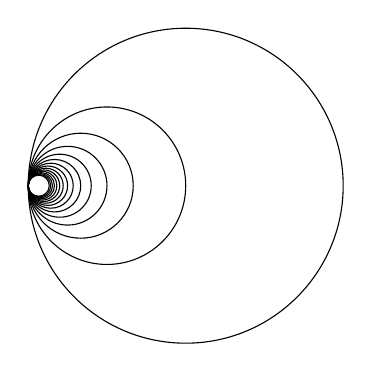
\begin{tikzpicture}
			\def \rad{2}
			\foreach \x in {1,...,15}
			{ \draw (\rad/\x, 0) circle (\rad/\x); }
		\end{tikzpicture}

		A depiction of $\displaystyle\bigcup_{n = 1}^{15}C_n$
	\end{center}

	\myfill

	To see this, consider the point $(0, 0) \in C.$ Given any $\delta > 0,$ there exists $n \in \mathbb{N}$ such that $C_n$ is completely contained in the $\delta$ neighbourhood of $(0, 0).$ Fix any such $n = n_0.$\\
	Consider the loop $\sigma$ starting at $(0, 0)$ and looping around $C_{n_0}$ once. Now, we need to show that $\sigma$ cannot be contracted to a point, \emph{even if we allow the loop to go outside} $U.$\\
	To do this, we consider the map $p:(C, (0, 0)) \to (S^1, (1, 0))$ which maps $C_{n_0}$ to $S^1$ in the natural way and collapses everything else to $(1, 0).$\\
	(It can be verified that this is a continuous function.)\\
	Now, we see that $p_*:\pi_1(C, (0, 0)) \to \pi_1(S^1, (1, 0))$ maps $[\sigma]$ to the generator of $\pi_1(S^1, (1, 0)).$ In particular, $[\sigma]$ is not trivial (in $C,$ not just in $U$).
\end{ex}

\subsection{Constructing the universal covering space}
\begin{thm}
	If $X$ is a semi-locally simply connected (and path-connected and locally path-connected) space, then $X$ has a universal covering.
\end{thm}
In this subsection, we give a proof of this theorem by constructing a universal covering. We shall fix $X$ to be as in the theorem.\\
%
%
\begin{proof} \phantom{hi}\\
\textsc{Step 1.} \textbf{Constructing the set $\tilde{X}.$}\\
Choose $x_0 \in X.$ We consider the set $S$ all paths in $X$ with initial point $x_0.$ Define $\sim$ on $S$ by $\alpha \sim \beta$ if $\alpha\simeq\beta\rel\{0, 1\}.$ (In particular, $\alpha(1) = \beta(1).$)\\
% \rsnoteil{Something to tie into homotopy theory, this is called the Path spaces and if you look at the preimage of $x_0$ under the map $p$ you will get the space of loops at $x_0$ ($\Omega_{x_0} X$. This is known as the path loop fibration. A fibration is characterised by a lifting criterion which allows you to lift higher homotopies as well. Just putting it in here so you can relate to homotopy theory material we do later. }
Let $\langle \alpha\rangle$ be the equivalence class of $\alpha.$ We define
\begin{equation*} 
	\tilde{X} = S/{\sim} = \{\langle \alpha\rangle \mid \alpha \in S\}.
\end{equation*}

\dotfill

\textsc{Step 2.} \textbf{Giving $\tilde{X}$ a topology - defining a basis.}\\
Let $V$ be a neighbourhood of $\alpha(1).$ We define $\langle a, V\rangle$ to be the set of all $\langle \alpha\beta\rangle$ where $\beta$ is a path in $V$ with initial point $\alpha(1).$\\
Let $\mathcal{B}$ be the set of all $\langle \alpha, V\rangle$s. We show that $\mathcal{B}$	is a basis.\\
Note that $\langle \alpha\rangle \in \langle \alpha, X\rangle$ and thus, every element of $\tilde{X}$ does indeed belong to an element of $\mathcal{B}.$\\
Now, suppose $\langle \alpha''\rangle \in \langle \alpha, V\rangle \cap \langle \alpha', V'\rangle.$ In particular, $\langle \alpha''\rangle \in \langle \alpha, V\rangle$ which gives that $\alpha''(1) \in V.$ Thus, $V$ is a neighbourhood of $\alpha''(1)$ as well. Moreover, if 
\begin{equation*} 
	\alpha'' \simeq \alpha\beta\rel\{0, 1\}
\end{equation*} 
for some path $\beta$ in $V,$ then 
\begin{equation*} 
	\alpha \simeq \alpha''\beta^{-1}\rel\{0, 1\}
\end{equation*} with $\beta'$ again being in $V.$\\
Thus, we see that $\langle \alpha'', V\rangle = \langle \alpha, V\rangle.$\\
Similarly, $\langle \alpha'', V'\rangle = \langle \alpha', V'\rangle.$ Now,
\begin{equation*} 
	\langle \alpha, V\cap V'\rangle \subset\langle \alpha'', V\rangle\cap\langle \alpha'', V'\rangle
\end{equation*}
or
\begin{equation*} 
	\langle \alpha''\rangle \in \langle \alpha'', V\cap V'\rangle \subset\langle \alpha, V\rangle\cap\langle \alpha', V'\rangle,
\end{equation*}
proving that $\mathcal{B}$ is a basis.\\
Of course, we now give $\tilde{X}$ the topology generated by $\mathcal{B}.$

\dotfill

\textsc{Step 3.} \textbf{Defining the map $p$.}\\
Define
\begin{equation*} 
	p:\tilde{X} \to X
\end{equation*}
as
\begin{equation*} 
	p\langle \alpha\rangle = \alpha(1).
\end{equation*}
(Clearly, this is well-defined.)\\
To show that this is a map, that is, it is continuous, note that given any $\langle \alpha\rangle$ and any open set $V$ containing $\alpha(1),$ the set $p\langle \alpha, V\rangle$ is the path component of $\alpha(1)$ in $V.$ (Note that the path component of $\alpha(1)$ in $V$ is precisely the set of all those points $x$ such that there's a path $\alpha(1) \overset{\beta}{\longrightarrow}x.$ Then, $x = p\langle \alpha\beta\rangle \in p\langle \alpha, V\rangle.$)\\
Thus, given any $\langle \alpha\rangle \in \tilde{X}$ and neighbourhood $V$ of $p\langle \alpha\rangle,$ we have that the neighbourhood $\langle \alpha, V\rangle$ of $\langle \alpha\rangle$ gets mapped in $V.$ This shows that $p$ is continuous. In fact, this also shows that $p$ is open since basis elements get mapped to open sets. (Path components are connected components (since $X$ is locally path-connected) which are open.)

\dotfill

\textsc{Step 4.} \textbf{Showing that $\tilde{X} \overset{p}{\longrightarrow} X$ is a covering map.}\\
Given $x \in X,$ choose a \emph{path-connected} neighbourhood $V$ of $x$ such that any loop at $x$ in $V$ can be shrunk to $x$ in $X.$ (We use the fact that $X$ is locally path-connected and semi-locally simply connected.) \\
We show that $V$ is evenly covered. \\
Let $\alpha$ be any path starting at $x_0$ such that $p\langle \alpha\rangle \in V.$ (Such a path does exist since $X$ is path-connected and so, there exists $x_0\overset{\alpha}{\longrightarrow} x \in V.$) \\
\begin{blockquote}
	\textbf{Claim 1.} $p\langle \alpha, V\rangle = V.$
	\begin{proof} 
		It follows by our previous observation that $p\langle \alpha, V\rangle \subset V.$ We have equality this time since $V$ is path-connected.
	\end{proof}
\end{blockquote}
We show that $p$ maps $\langle \alpha, V\rangle$ homeomorphically onto $V.$\\
Well, we have already shown that it is \emph{onto.} We had also shown that this is continuous and open. Thus, all we need to show that this one-one. For then, it would follow that it is a bijection and that the inverse is also continuous. (By virtue of it being open.)\\
Suppose that $p\langle \alpha\beta\rangle = p\langle \alpha\beta'\rangle.$ (Note that $\langle \alpha\beta\rangle$ is a typical element of $\langle \alpha, V\rangle$ where $\beta$ is a path in $V$ starting at $\alpha(1)$.)\\
Then, $\beta$ and $\beta'$ have the same terminal points (and of course, initial points as well). Note that $\beta\beta'^{-1}$ is a loop at $x.$ By choice of $V,$ we have
\begin{equation*} 
	\beta\beta^{-1} \simeq e_x \rel\{0, 1\}
\end{equation*}
or
\begin{equation*} 
	\alpha\beta \simeq \alpha\beta' \rel\{0, 1\}
\end{equation*}
giving
\begin{equation*} 
	\langle \alpha\beta\rangle = \langle \alpha\beta'\rangle,
\end{equation*}
as desired.

Moreover, note that the complete preimage of $V$ is the disjoint union of all $\langle \alpha, V\rangle$ such that $p\langle \alpha\rangle \in V.$ (That this is the complete preimage is obvious.) \\
To see that the union is disjoint, suppose $\alpha$ and $\alpha'$ are paths such that $\langle \alpha, V\rangle \cap \langle \alpha', V\rangle \neq \emptyset.$ Then, for $\langle \alpha''\rangle$ in the intersection, we have
\begin{equation*} 
	\langle \alpha, V\rangle = \langle \alpha'', V\rangle = \langle \alpha', V\rangle,
\end{equation*} 
as earlier, showing that the union is disjoint.\\
Thus, this is the decomposition of $p^{-1}(V)$ into sheets, as desired.

\dotfill

\textsc{Step 5.} \textbf{$\tilde{X}$ is path-connected.}\\
Let $\widetilde{x_0} = \langle e_{x_0}\rangle,$ the class of the constant loop at $x_0.$ We show that we can join any point $\langle \alpha\rangle \in \tilde{X}$ to $\widetilde{x_0}$ which would show that $\tilde{X}$ is path-connected.\\
Given a path $x_0 \overset{\alpha}{\longrightarrow} x$ in $X,$ define
\begin{equation*} 
	\alpha_s(t) = \alpha(st), \quad s, t \in I.
\end{equation*}
Thus, for each $s \in I,$ $\alpha_s$ is a path in $X$ such that $\alpha_s(0) = \alpha(0) = x_0.$ That is, each $\alpha_s$ is a path starting at $x_0.$\\
Now, define $\tilde{\alpha}:I \to \tilde{X}$ as 
\begin{equation*} 
	\tilde{\alpha}(s) := \langle \alpha_s\rangle.
\end{equation*}
Note that $\alpha_0$ is the constant loop at $x_0$ and $\alpha_1 = \alpha.$ Thus, we have that 
\begin{equation*} 
	\widetilde{x_0} \overset{\tilde{\alpha}}{\longrightarrow} \langle \alpha\rangle
\end{equation*}
is a path in $\tilde{X},$ provided we show that $\tilde{\alpha}$ is continuous.\\
To see this, let $s_0 \in I$ be arbitrary and consider a basis neighbourhood $\langle \alpha_{s_0}, V\rangle$ of $\tilde{\alpha}(s) = \alpha_s.$\\
Note that $\alpha_{s_0}(1) \in V,$ that is, $\alpha(s_0) \in V.$ Since $\alpha$ is continuous, there exists a $\delta$-neighbourhood $U$ around $s_0$ such that $\alpha(U) \subset V.$\\
We show that $\tilde{\alpha}(U) \subset \langle \alpha_{s_0}, V\rangle.$\\
To see this, let $s \in U.$ Then,
\begin{equation*} 
	p\langle \alpha_s\rangle = \alpha_s(1) = \alpha(s) \in V.
\end{equation*}
Let $s_M = \max\{s, s_0\}$ and $s_m = \min\{s, s_0\}.$ \\
Then, note that the $\alpha_{s_M}$ is a path which can be seen as a product of the path $\alpha_{s_m}$ with a path joining the point $\alpha(s_m)$ to $\alpha(s_M),$ the latter lying completely in $V$ since $\alpha(U) \subset V.$\\
Thus, we see that $\langle \alpha_{s_M}\rangle \in \langle \alpha_{s_m}, V\rangle$ and vice-versa. Since $\{s_m, s_M\} = \{s, s_0\},$ we see that
\begin{equation*} 
	\tilde{\alpha}(s) = \langle \alpha_s\rangle \in \langle \alpha_{s_0}, V\rangle,
\end{equation*}
as desired. This shows that $\tilde{\alpha}$ is continuous and thus, $\tilde{X}$ is path connected.\\
Moreover, we see that
\begin{equation*} 
	(p\circ\tilde{\alpha})(s) = p\langle \alpha_s\rangle = \alpha_s(1) = \alpha(s),
\end{equation*}
that is, $\tilde{\alpha}$ lifts $\alpha.$ 

\dotfill

\textsc{Step 6.} \textbf{$X$ is simply connected.}\\
We show that $\pi_1(\tilde{X}, \widetilde{x_0})$ is trivial.\\
Let $\tau$ be a loop in $\tilde{X}$ at $\widetilde{x_0},$ and let $\alpha = p \circ \tau.$ By uniqueness of lifts, we have
\begin{equation*} 
	\tau = \tilde{\alpha},
\end{equation*}
where $\tilde{\alpha}$ is defined as earlier. (Uniqueness since both $\tau$ and $\tilde{\alpha}$ have initial point $\widetilde{x_0}.$) \\
In particular, $\tilde{\alpha}$ is a loop at $\widetilde{x_0}$ (since so was $\tau$).\\
Thus, we have
\begin{equation*} 
	\langle \alpha\rangle = \langle \alpha_1\rangle = \tilde{\alpha}(1) = \widetilde{x_0} = \langle e_{x_0}\rangle.	
\end{equation*}
(The last equality was the definition of $\widetilde{x_0}.$)\\
Thus, we have
\begin{equation*} 
	\langle \alpha\rangle = \langle e_{x_0}\rangle
\end{equation*}
or that
\begin{equation*} 
	\alpha \simeq e_{x_0} \rel \{0, 1\}.
\end{equation*}
By the \nameref{thm:pathhomotlifts}, we see that 
\begin{equation*} 
	\tilde{\alpha} \simeq \widetilde{e_{x_0}} \rel\{0, 1\}.
\end{equation*}
Since we have $\tilde{\alpha} = \tau$ and $\widetilde{e_{x_0}} = e_{\widetilde{x_0}},$ we are done!
\end{proof}

The above then finishes our construction as we have shown that
\begin{equation*} 
	(\tilde{X}, \widetilde{x_0}) \overset{p}{\longrightarrow} (X, x_0)
\end{equation*}
is a covering space where $X$ is simply connected.

\begin{cor} \label{cor:galoiscorresp}
	Under the same hypothesis, for every subgroup $H$ of $\pi_1(X, x_0),$ there exists a covering space $(E, e_0) \overset{p}{\longrightarrow} (X, x_0),$ unique up to equivalence, such that $H = p_*\pi_1(E, e_0).$
\end{cor}
\begin{proof} 
	We sketch the proof: Let $(\tilde{X}, \widetilde{x_0})\overset{q}{\longrightarrow}(X, x_0)$ be the universal covering space with group of covering transformations $G.$ Then, $G \cong \pi_1(X, x_0)$ and $G$ acts evenly on $\tilde{X}.$\\
	Let $H' \le G$ be the subgroup corresponding to $H.$ Put $(E, e_0) \vcentcolon= (\tilde{X}/H', H'\widetilde{x_0}).$ Then, the quotient map $\tilde{X}\to E$ induces a covering map $p:(E, e_0) \to (X, x_0).$\\
	One then shows that $p_*\pi_1(E, e_0) = (X, x_0).$	

	Using the general Lifting Criterion (\cref{thm:liftcriterion}) four times, we get the uniqueness (up to equivalence) of $(E, e_0) \to (X, x_0).$
\end{proof}

We will now prove a result about topological groups, before which we prove a lemma.

\begin{lem} \label{lem:topgroupfundabel}
	Let $X$ be a topological group with operation $\cdot$ and identity element $x_0.$ Let $\Omega(X, x_0)$ denote the set of all loops at $x_0$ in $X.$ If $f, g \in \Omega(X, x_0),$ we define a loop $f\otimes g$ at $x_0$ by the rule
	\begin{equation*} 
		(f \otimes g)(s) = f(s)\cdot g(s).
	\end{equation*}
	\begin{enumerate}
		\item This operation makes $\Omega(X, x_0)$ into a group.
		\item This operation induces a group operation $\otimes$ on $\pi_1(X, x_0).$
		\item The two group operations $*$ and $\otimes$ on $\pi_1(X, x_0)$ are the same. (Recall that $*$ was the usual product of paths, in this case, loops.)
		\item $\pi_1(X, x_0)$ is abelian.
	\end{enumerate}
\end{lem}
\begin{proof} 
	\phantom{Hi}
	\begin{enumerate}
		\item This is a simple check. $\otimes$ is associative since $\cdot$ is. Moreover, $e_{x_0},$ the constant loop at $x_0$ acts as the identity as can be easily checked.\\
		Lastly, given $f\in\Omega(X, x_0),$ we see that $g:I\to X$ defined as
		\begin{equation*} 
			g(s) = (f(s))^{-1}
		\end{equation*}
		is an element of $\Omega(X, x_0)$ and is the (two-sided) inverse of $f$ with respect to $\otimes.$\\
		Thus, $\Omega(X, x_0)$ is a group under $\otimes.$
		\item In other words, we need to show that if $f \simeq f'$ and $g \simeq g',$ both $\rel \{0, 1\},$ then
		\begin{equation*} 
			f\otimes g \simeq f'\otimes g' \rel\{0, 1\}.
		\end{equation*}
		To see this, let $H:f\simeq f' \rel\{0, 1\}$ and $H':g\simeq g'\rel\{0, 1\}$ be path homotopies. We define a new path homotopy 
		\begin{equation*} 
			H\otimes H': I \times I \to X
		\end{equation*} given as
		\begin{equation*} 
			(H \otimes H')(s, t) = H(s, t)\cdot H'(s, t).
		\end{equation*}
		One can note that $(H\otimes H')(0, t) = x_0\cdot x_0$ and similarly for $(1, t).$\\
		Likewise, we have 
		\begin{equation*} 
			(H \otimes H')(s, 0) = H(s, 0)\cdot H'(s, 0) = f(s)\cdot g(s) = (f\otimes g)(s)
		\end{equation*}
		and similarly for $(s, 1).$\\
		This shows that $\otimes$ induces a group operation on $\pi_1(X, x_0).$ 
		\item To do this and the next part, we just show that
		\begin{equation*} 
			([f] \otimes [g]) * ([\sigma] \otimes [\tau]) = ([f] * [\sigma]) \otimes ([g] * [\tau])
		\end{equation*}
		for all $f, g, \sigma, \tau \in \Omega(X, x_0).$ The result will then follow from \nameref{thm:eckmannhilton}.\\
		Since both $*$ and $\star$ are compatible with $[\cdot],$ the above is equivalent to
		\begin{equation*} 
			[\underbrace{(f \otimes g)*(\sigma \otimes \tau)}_{=\vcentcolon \alpha}] = [\underbrace{(f * \sigma) \otimes (g * \tau)}_{=\vcentcolon\beta}].
		\end{equation*}
		Thus, if we show that $\alpha \simeq \beta \rel \{0, 1\},$ then we are done. In fact, we will show that $\alpha = \beta.$\\
		Indeed, we have
		\begin{align*} 
			\alpha(s) &= \left((f \otimes g)*(\sigma \otimes \tau)\right)(s)\\
			&= \begin{cases}
				(f\otimes g)(2s) & 0 \le 2s \le 1,\\
				(\sigma \otimes \tau)(2s - 1) & 1 \le 2s \le 2
			\end{cases}\\
			&= \begin{cases}
				f(2s)\cdot g(2s) & 0 \le 2s \le 1,\\
				\sigma(2s - 1)\cdot\tau(2s - 1) & 1 \le 2s \le 2.
			\end{cases}
		\end{align*}
		On the other hand, we have
		\begin{align*} 
			\beta(s) &= \left((f * \sigma) \otimes (g * \tau)\right)(s)\\
			&= \left((f*\sigma)(s)\right)\cdot\left((g*\tau)(s)\right)\\
			&= \begin{cases}
				f(2s)\cdot g(2s) & 0 \le 2s \le 1,\\
				\sigma(2s - 1)\cdot\tau(2s - 1) & 1 \le 2s \le 2.
			\end{cases}
		\end{align*}
		Thus, we see that $\alpha = \beta,$ as desired. \qedhere
	\end{enumerate}
\end{proof}

\begin{thm}
	If $X$ is a topological group with operation $\cdot$, then for any covering space $E \overset{p}{\longrightarrow} X$ and point $e_0$ in the fiber of the neutral element $x_0$ of $X,$ there is a unique structure of topological group on $E$ for which $e_0$ is the neutral element and $p$ is a homomorphism.
\end{thm}
\begin{proof} 
	Let $m:X\times X \to X$ be the map $(x_1, x_2) \mapsto x_1\cdot x_2.$ We wish to lift the red map $m\circ(p \times p)$ to a map $m'$ as shown.
	\begin{center}
		\begin{tikzcd}
		{(E \times E, (e_0, e_0))} \arrow[dd, "p\times p"', red] \arrow[rr, "m'", dashed] &  & {(E, e_0)} \arrow[dd, "p"] \\ &  & \\
		{(X \times X, (x_0, x_0))} \arrow[rr, "m"', red]&  & {(X, x_0)}                
		\end{tikzcd}
	\end{center}
	Once we do that, we would define $\cdot$ on $E$ as $e_1\cdot e_2^{-1} = m'(e_1, e_2).$ \\
	Note that any other structure would also make the above diagram commute (since $p$ is a homomorphism) and thus, $m'$ (if it exists) is unique. (By \nameref{thm:uniquelift}.)\\
	The criterion for its existence is 
	\begin{equation*} 
		m_*(p \times p)_*\pi_1(E \times E, (e_0, e_0)) \subset p_*\pi_1(E, e_0),
	\end{equation*}
	as given by \cref{thm:liftcriterion}.\\
	Let us first examine $m_*.$ Given $[\alpha] \in \pi_1(X\times X, (x_0, x_0)),$ we have
	\begin{equation*} 
		m_*([\alpha]) = [m \circ \alpha].
	\end{equation*}
	Note that any loop $\alpha$ at $(x_0, x_0)$ in $X \times X$ looks like
	\begin{equation*} 
		\alpha = \alpha_1 \times \alpha_2
	\end{equation*}
	for some loops $\alpha_1$ and $\alpha_2$ at $x_0$ in $X.$ Thus, we have
	\begin{equation*} 
		(m\circ\alpha)(t) = \alpha_1(t)\cdot(\alpha_2(t)), \quad t \in I.	
	\end{equation*}
	By the previous lemma, we conclude that
	\begin{equation*} 
		m\circ\alpha = \alpha_1*\alpha_2,
	\end{equation*}
	where the $*$ is the usual path (in this case, loop) product.\\
	Similarly, if $\sigma$ is a loop at $(e_0, e_0)$ in $E \times E,$ then $\sigma = (\sigma_1, \sigma_2)$ for some loops $\sigma_1, \sigma_2$ at $e_0$ in $E.$ Moreover, we have
	\begin{align*} 
		(p\times p)\circ\sigma = (p \circ \sigma_1)\times(p \circ \sigma_2).
	\end{align*}
	Thus,
	\begin{align*} 
		m\circ(p \times p) \circ \sigma &= (p \circ \sigma_1)*(p \circ \sigma_2)\\
		&= p \circ (\sigma_1 * \sigma_2)
	\end{align*}
	or
	\begin{equation*} 
		m_*(p\times p)_*[\sigma] = p_*[\sigma_1 * \sigma_2],	
	\end{equation*}
	showing that
	\begin{equation*} 
		m_*(p \times p)_*\pi_1(E\times E, (e_0, e_0)) \subset p_*(E_1, e_0),
	\end{equation*}
	fulfilling the lifting criterion.

	Thus, the lift $m'$ exists. We now show that it gives $E$ the structure of a topological group such that $e_0$ is the neutral element and $p$ is homomorphism.\\
	Define $\cdot:E\times E \to E$ as $e_1\cdot e_2 = m'(e_1, e_2).$\\
	We verify associativity using the following diagram:

	\begin{center}
		\begin{tikzcd}
			{E \times E \times E} \arrow[rr, "m' \times \id_E", red] \arrow[dd, "\id_E \times m'"', blue] & & {E \times E} \arrow[dd, "m'", red] & \\
			& & & \\
			{E \times E} \arrow[rr, "m' \times \id_E"', blue] & & {E} \arrow[dr, "p"] & \\
			& & & {X} 
		\end{tikzcd}
	\end{center}

	(Note that these are actually maps preserving the obvious base-points.)\\
	Associativity amounts to showing that the square above commutes. However, using associativity in $X,$ we know that the blue maps composed with $p$ equals the red maps composed with $p.$ Then, by the \nameref{thm:uniquelift}, we see that these two must be equal.

	We now show that $e_0$ is the identity. Consider the map $i:E \to E$ defined as
	\begin{equation*} 
		i(e) = e\cdot e_0 = m'(e, e_0).
	\end{equation*}
	It follows that $i(e_0) = e_0.$ We wish to show that $i = \id_E.$ \\
	Note that
	
	\begin{equation*} 
		(p\circ i)(e) = p(m'(e, e_0)) = m(p(e), p(e_0)) = m(p(e), x_0) = p(e).
	\end{equation*}
	
	In other words, $i$ is a lift of $p$ which agrees with $\id_E$ at $e_0.$ By uniqueness of lifts, we see that $i = \id_E$ as desired. Similarly, we also get that $e_0$ is the left identity.

	To construct inverses, we shall lift the inversion map $i_X:X \to X$ similar to how we had lifted $m.$ By a similar Eckmann-Hilton type argument, we see that the lifting criterion is satisfied and thus, there exists a map $i_E:E \to E$ such that $p\circ i_E = i_X\circ p$ and $i_E(e_0) = e_0.$\\
	Now, define $j:E \to E$ as
	
	\begin{equation*} 
		j(e) = e\cdot i_E(e) = m'(e, i_E(e)).
	\end{equation*}

	Note that $j(e_0) = e_0.$ We wish to show that $j$ is the constant map $e\mapsto e_0.$ The usual trick works. Indeed, we note

	\begin{equation*} 
		p(j(e)) = pm'(e, i_E(e)) = p(e)\cdot p(i_E(e)) = p(e)\cdot i_X(p(e)) = x_0.
	\end{equation*}

	Thus, $j$ is a lift of the constant map $e \mapsto x_0$ and so is the constant map $e_{e_0}.$ Since $j$ and $e_{e_0}$ at $e_0,$ they must be equal. (Similarly, this acts as a left inverse as well.)

	$m'$ and $i_E$ are lifts by construction and thus, are continuous. Thus, $E$ is a topological group with $e_0$ as identity. The fact that $p$ is a homomorphism also follows from construction since we have $p\circ m' = m\circ(p\times p).$
\end{proof}

\section{Van Kampen's Theorem} \label{sec:vankampen}
\subsection{Free Product of Groups}
We briefly describe the free product of groups and fix some notation. We shall not prove the basic facts about free groups. \\
Let $\{G_\alpha\}_{\alpha \in A}$ be a collection of (disjoint) groups. We denote the free product of the groups as
\begin{equation*} 
	*_\alpha G_\alpha.
\end{equation*}
(This is slight abuse of notation since we don't mention $A$ but there won't be any confusion.)

As a set, the free product $*_\alpha G_\alpha$ consists of words of the form
\begin{equation*} 
	g_1\cdots g_m
\end{equation*}
of arbitrary finite length $m \ge 0$ satisfying the following conditions:
\begin{enumerate}
	\item each letter $g_i$ belongs to a group $G_{\alpha_i},$
	\item $g_i$ is not the identity element of $G_{\alpha_i},$
	\item adjacent letters belong to different groups, i.e., $\alpha_i \neq \alpha_{i + 1}.$	
\end{enumerate}
Words satisfying these conditions are called \emph{reduced}. The idea being that an arbitrary word using with letters from $G_\alpha$ can be reduced to this type of word by combining letters and discarding the trivial (identity) letters.\\
The group operation of this group is juxtaposition, followed by reduction. The identity of this group is the empty word. (That is, the unique word of length $m = 0.$)

Given the free product $*_\alpha G_\alpha,$ each group $G_\alpha$ is naturally identified with the subgroup $*_\alpha G_\alpha$ that contains the empty word and non-identity one-letter words $g \in G.$\\
Under this identification, we now state the universal property of a free product.
\begin{thm}[Universal property]
	Given any collection $\{G_\alpha\}$ of groups and collection of (group) homomorphisms
	\begin{equation*} 
		\varphi_\alpha: G_\alpha \to H,
	\end{equation*}
	there exists a unique homomorphism
	\begin{equation*} 
		\varphi:*_\alpha G_\alpha \to H,
	\end{equation*}
	such that
	\begin{equation*} 
		\varphi|_{G_\alpha} = \varphi_\alpha,
	\end{equation*}
	for each $\alpha.$
\end{thm}

In others words, the homomorphisms $\varphi_\alpha:G_\alpha \to H$ \emph{extend} uniquely to a homomorphism $\varphi:*_\alpha G_\alpha \to H.$\\
This homomorphism is defined (on \emph{reduced} words) in the obvious manner by defining
\begin{equation*} 
	\varphi(g_1\cdots g_m) \vcentcolon= \varphi_{\alpha_1}(g_1)\cdot\cdots\cdot\varphi_{\alpha_m}(g_m).
\end{equation*}
%
%
%
\subsection{The Van Kampen Theorem}
Let $X$ be a topological space such that $X = \bigcup A_\alpha,$ where $A_\alpha$ are path-connected open subsets of $X,$ each of which contain a base-point $x_0 \in X.$ (We shall fix this base-point and not mention it when writing the fundamental groups.) \\
By the universal property in the previous subsection, we see that the homomorphism $j_\alpha:\pi_1(A_\alpha) \to \pi_1(X)$ induced by the inclusions $(A_\alpha) \hookrightarrow (X)$ extend to a homomorphism
\begin{equation*} 
	\Phi:*_\alpha\pi_1(A_\alpha) \to \pi_1(X).
\end{equation*}
Note, that the groups are not necessarily disjoint but we formally treat them to be disjoint in the free product.\\
To elaborate, if
\begin{equation*} 
	i_{\alpha\beta}:\pi_1(A_\alpha \cap A_\beta) \to \pi_1(A_\alpha)
\end{equation*}
is the homomorphism induced by the inclusion $A_\alpha\cap A_\beta \hookrightarrow A_\alpha,$ then
\begin{equation*} 
	j_{\alpha}\circ i_{\alpha\beta} = j_\beta\circ i_{\beta\alpha},
\end{equation*}
for both are the homomorphism induced by the inclusion $A_\alpha\cap A_\beta \hookrightarrow X.$\\
Thus, we would need $\Phi$ to agree on $i_{\alpha\beta}(w) \in \pi_1(A_\alpha)$ and $i_{\beta\alpha}(w) \in \pi_1(A_\beta)$ for $w \in \pi_1(A_\alpha\cap A_\beta).$ This tells us that the kernel of $\Phi$ should contain $i_{\alpha\beta}(w)i_{\beta\alpha}(w)^{-1}.$\\
Van Kampen's theorem asserts that under reasonable hypothesis, $\Phi$ is surjective and the above gives a complete description of the kernel.

\begin{thm}[The Van Kampen Theorem] \label{thm:vankampen}
	If $X$ is the union of path-connected open sets $A_\alpha$ each containing the base-point $x_0 \in X$ and if each intersection $A_\alpha \cap A_\beta$ is path-connected, then the homomorphism
	\begin{equation*} 
		\Phi:*_\alpha\pi_1(A) \to \pi_1(X)
	\end{equation*}
	is surjective. If in addition each intersection $A_\alpha\cap A_\beta\cap A_\gamma$ is path-connected, then the kernel of $\Phi$ is the normal subgroup $N$ generated by all elements of the form $i_{\alpha\beta}(w)i_{\beta\alpha}(w)^{-1},$ and so $\Phi$ induces a homomorphism
	\begin{equation*} 
		\pi_1(X) \cong *_\alpha\pi_1(A_\alpha)/N.
	\end{equation*}
\end{thm}

Note that \cref{thm:vankampenspecial} from earlier was a special case of the above general theorem. In fact, surjectivity of $\Phi$ was almost given in the proof there. We shall write some of it again in order to fix the notation consistently for this scenario.

\emph{Proof.}
	Given a loop $f:I \to X$ at the base-point $x_0,$ we claim (as usual) that there is a partition $0 = s_0 < s_1 < \cdots < s_m = 1$ of $I$ such that each subinterval $[s_{i - 1}, s_i]$ is mapped by $f$ into a single $A_\alpha.$ This, of course, follows from compactness of $I.$\\
	Denote that $A_\alpha$ containing $f([s_{i - 1}, s_i])$ by $A_i,$ and let $f_i$ be the path obtained by restricting $f$ to $[s_{i-1}, s_i]$ and reparameterising appropriately. As in the proof of \cref{thm:vankampenspecial}, we see that we can write
	\begin{equation*} 
		[f] = [f_1g_1^{-1}][g_1f_2g_2^{-1}]\cdots[g_{m-1}f_m],
	\end{equation*}
	where each $g_i$ is a path in $A_i\cap A_{i+1}$ from $x_0$ to the point $f(s_i) \in A_i\cap A_{i+1}.$\\
	The above then shows that $f$ is homotopic to a product of \emph{loops}, each of which lie in a single $A_i.$ Hence, $[f]$ is in the image of $\Phi$ and $\Phi$ is surjective.\\
	(Recall the extension of homomorphisms as given by the universal property.)

	\dotfill

	Now, we prove the harder part, namely that $N$ is the kernel of the homomorphism $\Phi.$\\
	Firstly, we note that $N$ must be contained in $\ker \Phi.$ Given any $\alpha, \beta$ and $w \in \pi_1(A_\alpha)\cap\pi_1(B_\alpha),$ we recall we had seen that
	\begin{equation*} 
		(j_{\alpha}\circ i_{\alpha\beta})(w) = (j_{\beta}\circ i_{\beta\alpha})(w).
	\end{equation*}
	Thus, we must have $\Phi(i_{\alpha\beta}(w)) = \Phi(i_{\beta\alpha}(w)).$ (Since $\Phi$ was extending the $j_\alpha$s.)\\
	Thus, $\ker\Phi$ is a normal subgroup that contains elements of the form
	\begin{equation*} 
		i_{\alpha\beta}(w)i_{\beta\alpha}(w)^{-1}.
	\end{equation*}
	Since $N$ was the smallest such, we see that $N \le \ker\Phi.$

	The above then gives us that $\Phi$ induces a map
	\begin{equation*} 
		Q = *_\alpha G_\alpha/N \to \pi_1(X).
	\end{equation*}

	To show that $N$ is exactly the kernel, we will show that the above map is injective. We now introduce some terminology.\\
	By a \emph{factorisation} of an element $[f] \in \pi_1(X),$ we shall mean a formal product $[f_1]\cdots[f_k]$ where
	\begin{enumerate}
		\item Each $f_i$ is a loop in some $A_\alpha$ with base-point $x_0,$ and $[f_i] \in \pi_1(A_\alpha)$ is the homotopy class of $f_i.$
		\item The loop $f$ is homotopic to $f_1*\cdots*f_k$ in $X.$
	\end{enumerate}
	In other words, $[f_1]\cdots[f_k]$ is a word in $*_\alpha \pi_1(A_\alpha),$ \emph{not necessarily reduced.} \\
	(Note that for each factorisation, we are keeping track of which group $[f_i]$ lies in. In particular, even if $f_i$ lies in some intersection $A_\alpha \cap A_\beta,$ we get two different factorisations by considering it as $[f_i]$ lying in two different groups.) \\
	Moreover, it is a word which gets mapped to $[f]$ under $\Phi.$ The proof of surjectivity earlier shows that each $[f]$ does have a factorisation. \\
	Now, we introduce an \emph{equivalence} of factorisations. Call two factorisations of $[f]$ \emph{equivalent} if they are related by a finite sequence of following two sorts of moves or their inverses:
	\begin{enumerate}
		\item Combine adjacent terms $[f_i][f_{i+1}]$ into a single term $[f_i*f_{i+1}]$ if $[f_i]$ and $[f_{i+1}]$ lie in the same group $\pi_1(A_\alpha).$
		\item Regard the term $[f_i] \in \pi_1(A_\alpha)$ as lying in the group $\pi_1(A_\beta)$ rather than $\pi_1(A_\alpha)$ if $f_i$ is a loop in $A_\alpha \cap A_\beta.$
	\end{enumerate}
	The first move (and its inverse) clearly does not change the element viewed as an element of $*_\alpha\pi_1(A_\alpha)$ since that is just applying the group operation on it.\\
	The second move does change it as an element of $*_\alpha\pi_1(A_\alpha).$ However, it does \emph{not} change it as an element of the \emph{quotient group} $Q = *_\alpha\pi_1(A_\alpha)/N.$\\
	In other words, equivalent factorisations give same elements of $Q.$

	Note that we had shown that $\Phi$ induces a homomorphism $Q \to \pi_1(X).$ If we show that any two factorisations of $[f]$ are equivalent, we shall get that 
	\begin{equation*} 
		\Phi(a) = \Phi(b) \implies a \text{ and } b \text{ are equivalent.}
	\end{equation*} 
	In other words, $a$ and $b$ are equal modulo $N.$ In yet other words, the map $Q \to \pi_1(X)$ is injective and thus, $N$ is precisely the kernel of $\Phi.$

	Let $[f_1]\cdots[f_k]$ and $[f_1']\cdots[f_l']$ be two factorisations of $[f].$ The composed paths $f_1*\cdots*f_k$ and $f_1'*\cdots*f_l'$ must then be homotopic to $f$ and hence, to each other.\\
	Let $F:I\times I \to X$ be a path homotopy from the former to the latter. As usual, there exist partitions $0 = s_0 < s_1 < \cdots < s_m = 1$ and $0 = t_0 < t_1 < \cdots < t_n = 1$ such that each rectangle $R_{ij} = [s_{i-1}, s_i]\times[t_{j-1}, t_j]$ is mapped by $F$ into a single $A_\alpha,$ which we denote by $A_{ij}.$\\
	Moreover, we may assume that the $s$-partition further subdivides the partitions that give the products $f_1*\cdots*f_k$ and $f_1'*\cdots*f_l'.$ That is, each $f([s_{i-1}, s_i])$ lies completely in some $A_\alpha$ in which one of the $f_j$ or $f_j'$ lie.

	\begin{wrapfigure}{r}{0pt}
		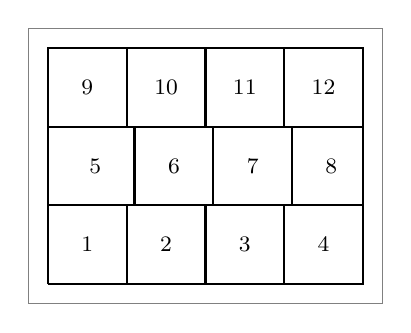
\begin{tikzpicture}
	\def \len{1}
	\def \eps{0.1}
	\def \del{0.25}
	\draw[thin, gray] (-\del, -\del) -- (-\del, 3*\len+\del) -- (4*\len+\del, 3*\len+\del) -- (4*\len+\del, -\del) -- (-\del, -\del);
	\draw[thick] (0, 0) -- (0, 3*\len) -- (4*\len, 3*\len) -- (4*\len, 0) -- (0, 0);	
	\draw[thick] (0, \len) -- (4*\len, \len);
	\draw[thick] (0, 2*\len) -- (4*\len, 2*\len);
	\foreach \x in {1,...,3}
	{ \draw[thick] (\x*\len, 0) -- (\x*\len, \len);
	  \draw[thick] (\x*\len+\eps, \len) -- (\x*\len+\eps, 2*\len);
	  \draw[thick] (\x*\len, 2*\len) -- (\x*\len, 3*\len);
	}
	\foreach \x in {0,...,11}
	{
	  	\pgfmathparse{int(floor(\x/4))};
  		\let\row\pgfmathresult
  		\pgfmathparse{int(\x - 4*\row)};
  		\let\col\pgfmathresult
  		\pgfmathparse{int(\x + 1)};
  		\let\y\pgfmathresult
  		\pgfmathparse{int(\row - 2*floor(\row/2))};
  		\let\rem\pgfmathresult
		\node[] at ({(\col + 0.5)*\len + \rem*\eps}, {(\row + 0.5)*\len}) {\footnotesize\y};
	}
\end{tikzpicture}
	\end{wrapfigure}

	Since each $R_{ij}$ is compact and gets mapped into $A_{ij},$ there is a neighbourhood of $R_{ij}$ which gets mapped into $A_{ij}.$ Thus, we may slightly perturb the vertical edges of the rectangles $R_{ij}$ so that each point of $I\times I$ lies in at most three $R_{ij}$s. 
	We may also assume that $n \ge 3,$ so that there are at least three rows of rectangles. In this case, we may perturb each row in a way that the topmost and bottommost rows remain unperturbed. We relabel these new rectangles as $R_1,\allowbreak R_2,\allowbreak \ldots,\allowbreak R_{mn}$ and ordering them as in the figure. (For which we have $m = 4, n = 3.$)

	\begin{wrapfigure}{r}{0pt}
		\input{tikz-files/vkamp-2}
	\end{wrapfigure}

	If $\gamma$ is a path in $I\times I$ from the left edge to the right edge, then $F\circ\gamma$ is a loop in $X$ with base-point $x_0.$ (Recall that $F$ was a path homotopy and thus, maps both the left and right edges to $x_0.$)\\
	Let $\gamma_r$ be the path in $I \times I$ (from the left edge to the right) separating the first $r$ rectangles from the rest. ($\gamma_6$ has been depicted in the figure.)

	In particular, $\gamma_0$ is the bottom edge of $I\times I$ and $\gamma_{mn}$ the top edge.\\
	Also, note that we move from $\gamma_r$ to $\gamma_{r+1}$ by ``pushing'' across the rectangle $R_{r+1}.$ (See the next figure.)

	\begin{wrapfigure}{r}{0pt}
		\input{tikz-files/vkamp-3}
	\end{wrapfigure}

	We shall call the corners of $R_r$s \emph{vertices}. For each vertex $v,$ let $g_v$ be a path from $x_0$ to $F(v).$ By our construction $F(v)$ and $x_0$ both lie in the intersection of the two or three $A_{ij}$s corresponding to the $R_r$s containing $v.$ Thus, we can choose $g_v$ to also lie in this intersection since the theorem's hypothesis said that two or three of these intersections are path-connected. (This is why we had done the perturbation.)\\
	Thus, given the \emph{loop} $F\circ\gamma_r:I \to X,$ we may insert the paths $g_v^{-1}g_v$ at successive vertices, as in the proof of surjectivity. This gives us a factorisation of $[F\circ\gamma_r],$ where each of the factor corresponds to a vertical or horizontal segment along with the $g_v$s padded on either side to make it a loop.\\
	This factor can be regarded as an element of either of the $\pi_1(A_{ij})$ containing it. Different choices will still give equivalent factorisations.

	The more important observation now is that factorisations associated to $\gamma_r$ and $\gamma_{r+1}$ are also equivalent. When changing the factors from $F\circ\gamma_r$ to $F\circ\gamma_{r+1},$ the paths changed are homotopic via a homotopy in $R_{r+1}.$ Thus, this is change will be equivalent as this is just a change obtained by the group operation in $\pi_1(A_{ij}),$ where $A_{ij}$ is the set corresponding to $R_i.$ \\
	(To see this clearly, note the two blue paths (viewed as paths in $X$) in the figures are homotopic (including the $g_v$ paddings), using \cref{lem:gbad}.)

	Thus, we get that all the factorisations associated to each $\gamma_r$ are equivalent. We now show that can we can associate a factorisation to $\gamma_0$ which is equivalent to $[f_1]\cdots[f_k].$\\
	First, we identity the bottom edge $I\times\{0\}$ with $I$ in the natural way. Consider the path $f_1*\cdots*f_k$ with domain $I.$\\
	Note that each vertex in the bottom edge lies in at most two rectangles. Thus, for each such $v,$ we can choose a path $g_v$ as earlier to not only lie in the corresponding $A_{ij}$s of the rectangles but also in the $A_\alpha$ corresponding to the $f_i$ containing the $v$ in its domain. Thus, as earlier, we split $[f_1]\cdots[f_k]$ as $[f_1g_1^{-1}]\cdots[g_{k-1}f_k].$\\
	This is a factorisation associated to $\gamma_0$ which is equivalent to $[f_1]\cdots[f_k].$\\
	Similarly, we get a factorisation associated to $\gamma_{mn}$ which is equivalent to $\allowbreak[f_1']\cdots[f_l'].$ By our earlier observations, we are done. \hfill $\qed$

%
%
%
%

\section{Loop Spaces and Higher Homotopy Groups}
% \amnote{Reminder about contractible and based point contractible} \rsnote{ Some books just take contractibility  to be based in this case, however I think there is a way to adapt lemma 3.3 and use the idea about non-degenerate based point to get that contractible will imply the homotopy groups are trivial. }
\subsection{Loop Spaces}
Let $X$ be an arbitrary topological space and $X^I$ be the set of all maps from $I$ to $X.$ In other words, $X^I$ is the set of all paths in $X.$ (Recall that by ``maps'' and ``paths,'' we always mean \emph{continuous} functions.)\\
We wish to turn $X^I$ into a topological space. We wish to do this with no assumptions on $X.$ For this reason, we first define the sets
\begin{equation*} 
	[K, U] = \{\sigma \in X^I : \sigma(K) \subset U\},
\end{equation*}
where $K \subset I$ is compact and $U \subset X$ is open.\\
Note that the collection of all such $[K, U]$ form a subbasis for a topology on $X^I.$ (Recall that this just means that the union of all such sets equals $X^I.$)\\
To see this, take $K = I$ and $U = X$ itself.

\begin{defn}[Compact open topology]
	The topology on $X^I$ generated by the subbasis
	\begin{equation*} 
		\{[K, U]\subset X^I : K \subset I \text{ compact, } U \subset X \text{ open}\}
	\end{equation*}
	is called the \emph{compact-open topology}.
\end{defn}

Recall that the above means that the sets which are open in $X^I$ are precisely those which can be written as a union of finite intersections of elements of the form $[K, U].$ 

The main property that we shall by using of this topology is the following:

\begin{prop}[Evaluation is continuous] \label{prop:evaluationcontinuous}
	The evaluation map $\omega:X^I \times I \to X$ given by
	\begin{equation*} 
		\omega(\sigma, t) = \sigma(t)
	\end{equation*}
	is continuous.
\end{prop}

\begin{proof} 
	Let $(\sigma_0, t_0) \in X^I\times I$ be arbitrary and $V \subset X$ be a neighbourhood of $\omega(\sigma_0, t_0) = \sigma_0(t_0).$\\
	We wish to find a neighbourhood of $(\sigma_0, t_0)$ that is mapped into $V$ via $\omega.$\\
	Since $\sigma$ is continuous and $V$ is open, there exists an open interval $U$ of $t_0$ such that $\sigma(U) \subset V.$ We may find a smaller bounded open interval such that $\overline{W} \subset U.$ Note that $\overline{W}$ is compact. \\
	Note that $[\overline{W}, V]$ is one of the subbasis elements of $X^I$ and hence, is open. Thus, $T = [\overline{W}, V]\times W$ is a neighbourhood of $(\sigma_0, t_0).$\\
	Now, if $(\sigma', t') \in T,$ then $\sigma'(t') \in V$ since $\sigma' \in [\overline{W}, V]$ maps $W$ into $V.$ In other words, $\omega(\sigma', t') \in V,$ as desired. ($T$ is the desired neighbourhood that gets mapped in $V$ by $\omega.$)
\end{proof}

\begin{prop}[Bijective correspondence]\label{prop:bijectivecorresp}
	Let $X$ and $Y$ be topological spaces. There is a bijective correspondence between maps
	\begin{equation*} 
		f:Y\to X^I \quad \text{and} \quad F:Y\times I \to X.
	\end{equation*}
	The bijection is the one induced by relating $f$ and $F$ as
	\begin{equation*} 
		f(y)(t) = F(y, t).
	\end{equation*}
\end{prop}

\begin{proof} 
	It is clear that the above relation gives a bijection between \emph{functions} $Y\overset{f}{\longrightarrow}X^I$ and $Y\times I\overset{F}{\longrightarrow}X.$ Now, we show that it restricts to continuous functions.

	Firstly, assume that $f$ is continuous. Note that $F$ can be factorised as

	\begin{equation*} 
		I \times I \overset{f \times \id_I}{\longrightarrow} \Omega_{x_0}\times I \overset{\omega}{\longrightarrow} X.
	\end{equation*}

	By the earlier proposition, we see that $F$ is continuous.

	Conversely, assume that $F$ is continuous. To show that $f$ is continuous, it suffices to show that $f^{-1}([K, U])$ is open for any arbitrary subbasis element $[K, U] \subset X^I.$\\
	Choose $y \in f^{-1}([K, U]).$ \\
	This means that given any $k \in K \subset I,$ we have $f(y)(k) \in U$ or $F(y, k) \in U.$ Thus, we see that $F(\{y\} \times K) \subset U.$\\
	Since $F$ is continuous, there exist open sets $V \subset Y$ and $W \subset X$ such that $y \in V$ and $K \subset W$ with the property that $F(V \times W) \subset U.$ \\
	Now, note that if $y' \in V$ and $k \in K \subset W,$ then $f(y')(k) = F(y, k) \in U.$ In other words
	\begin{equation*} 
		f(y') \in [K, U].
	\end{equation*}
	This shows that $f$ maps $V$ into $[K, U]$ proving that $f^{-1}([K, U])$ is open. 
\end{proof}

We will now turn our attention to a specific subspace of $X^I.$

\begin{defn}
	Let $X$ be a topological space and $x_0 \in X.$ The subspace
	\begin{equation*} 
		\Omega_{X, x_0} = \Omega_{x_0}
	\end{equation*}
	is the subspace consisting of all \emph{loops} at $x_0$ in $X.$
\end{defn}

(The $X$ in the subscript is omitted since the ambient space will be usually be clear from context.)

\begin{prop}[Characterising the path connected components]
	$\sigma, \tau \in \Omega_{x_0}$ are in the same path-connected components iff $\sigma \simeq \tau \rel \{0, 1\}.$
\end{prop}
\begin{proof} 
	Given a path $f:I\to X^I,$ we get a function $F:I\times I \to X$ and vice-versa by the relation
	\begin{equation*} 
		f(s)(t) = F(s, t).
	\end{equation*}
	As we saw in \cref{prop:bijectivecorresp}, $f$ is continuous iff $F$ is.

	Now, if $f$ is a path from $\sigma$ to $\tau$ in $\Omega_{x_0},$ then $F$ can be verified to be a homotopy. Indeed, one notes that
	\begin{equation*} 
		F(0, t) = f(0)(t) = \sigma(t), \quad \text{ for all } t \in I.
	\end{equation*}
	Same follows for $F(1, t).$\\
	Moreover, since $f(s) \in \Omega_{x_0}$ for each $s \in I,$ we see that
	\begin{equation*} 
		F(s, 0) = f(s)(0) = x_0 = f(s)(1) = F(s, 1), \quad \text{ for all } s \in I.
	\end{equation*}
	Thus, $F:\sigma\simeq\tau\rel\{0, 1\}.$

	Conversely, if $F$ is a path homotopy, then $f$ defined above is seen to clearly satisfy $f(0) = \sigma$ and $f(1) = \tau.$ Moreover, one notes that $f(s)(0) = x_0 = f(s)(1)$ for all $s \in I.$ This shows that $f$ indeed maps into $\Omega_{x_0},$ completing the proof.
\end{proof}

\begin{cor}
	As a set, $\pi_1(X, x_0)$ is the set of path-connected components of $\Omega_{x_0}.$
\end{cor}
% \rsnote{A more general statement would be to say that the homotopy classes of maps $[X,Y]$ is the set of path components of $F(X,Y)$}

\begin{proof} 
	If $C \in \pi_1(X, x_0),$ then $C$ is the homotopy class of some loop $\sigma$ in $X$ based at $x_0.$ By the above proposition, it contains precisely those loops which are in the path connected component of $\sigma.$ This shows 
	\begin{equation*} 
		\pi_1(X, x_0) \subset \{\text{path-connected components of }\Omega_{x_0}\}.
	\end{equation*}

	Similarly, the reverse inclusion follows.
\end{proof}

The multiplication of loops defines a map $*:\mathcal{M}\to X^I,$ where $\mathcal{M}$ is the subset of $X^I \times X^I$ for which the usual $*$ is defined. (That is, all those $(\sigma, \tau)$ such that $\sigma(1) = \tau(0).$)

\begin{prop}
	The map $*:\mathcal{M}\to X^I$ is continuous.
\end{prop}

\begin{proof} 
	Recall that given paths $(\sigma, \tau) \in \mathcal{M},$ the path $\sigma*\tau \in X^I$ is defined as
	\begin{equation*} 
		(\sigma*\tau)(s) \vcentcolon= \begin{cases}
			\sigma(2s) & 0 \le 2s \le1,\\
			\tau(2s - 1) & 1 \le 2s \le 2.
		\end{cases}
	\end{equation*}

	Let $[K, U] \subset X^I$ be an arbitrary subbasic element. Define
	\begin{equation*} 
		K_1 = K \cap \left[0, \dfrac{1}{2}\right], \quad K_2 = K \cap \left[\dfrac{1}{2}, 1\right]
	\end{equation*}
	and
	\begin{equation*} 
		K_1' = 2K_1, \quad K_2' = 2K_2 - 1,
	\end{equation*}
	where the above operations have the natural meaning.\\
	Note that $K_1'$ and $K_2'$ are both compact subsets of $I.$\\
	Thus, $[K_1', U] \times [K_2', U]$ is an open subset of the domain and thus, continuity follows since
	\begin{equation*} 
		*^{-1}([K, U]) = [K_1', U] \times [K_2', U]. \qedhere
	\end{equation*}
\end{proof}	

As usual, we have a particular subset of $\mathcal{M}$ which is of interest, namely, $\Omega_{x_0} \times \Omega_{x_0}.$ Note that $*$ restricts to a binary operation on $\Omega_{x_0}.$ This gives us the following corollary.

\begin{cor}
	The map $*:\Omega_{x_0}\times\Omega_{x_0}\to\Omega_{x_0}$ is continuous.
\end{cor}

As usual, we will drop $*$ when it is clear from context. Let $C \in \Omega_{x_0}$ be the constant loop at $x_0.$ Then, we have $CC = C.$ \\
Note very carefully that $C$ does not act as an identity (in the general sense). Moreover, the multiplication is not associative (in the general sense). This is because we're taking the loops themselves and \emph{not} homotopy classes. However, we do have the following proposition.

Define $L_C, R_C : \Omega_{x_0} \to \Omega_{x_0}$ to be left and right multiplication by $C,$ respectively.

\begin{prop}
	$L_C$ is homotopic to the identity map of $\Omega_{x_0}$ relative to $\{C\}.$
\end{prop}

\begin{proof} 
	We do know (by \cref{lem:leftid}) that 
	\begin{equation*} 
		\sigma\simeq C\sigma\rel\{0, 1\},
	\end{equation*}
	for every $\sigma\in\Omega_{x_0}.$ We had the explicit homotopy $F_{\sigma}:I\times I \to X$ as

	\begin{equation*} 
		F_\sigma(s, t) =\begin{cases}
			x_0 & 0 \le 2s \le t,\\~\\
    	\sigma\left(\dfrac{2s - t}{2 - t}\right) & t \le 2s \le 2.
		\end{cases}
	\end{equation*}

	Now, use this to define $F:\Omega_{x_0} \times I \times I \to X$ by
	\begin{equation*} 
		F(\sigma, s, t) = F_{\sigma}(s, t).
	\end{equation*}
	That is above map is continuous can be seen by an application of the \nameref{thm:pastinglemma} and the fact that \nameref{prop:evaluationcontinuous}.

	Using this, we define the function $H:\Omega_{x_0}\times I \to\Omega_{x_0}$ as
	\begin{equation*} 
		H(\sigma, t)(s) = F(\sigma, s, t).
	\end{equation*}
	(Note carefully that we are defining $H$ by defining $H(\sigma, t)$ to be the loop which is given by the above. Another way to have written it could be $H(\sigma, t) = F_{\sigma}(-, t).$)

	By the \nameref{prop:bijectivecorresp} of earlier, we see that $H$ is indeed a continuous map into $X^I.$ Since $F_{\sigma}$ was a homotopy for all $\sigma,$ we get that each $H(\sigma, t)$ is actually a loop, that is, $H$ does map into $\Omega_{x_0}.$
	All that we need to verify now is that $H$ is a homotopy relative to $\{C\}.$

	First, note that $H(\sigma, 0) = \sigma = \id_{\Omega_{x_0}}(\sigma)$ and $H(\sigma, 1) = C\sigma = L_C(\sigma).$\\
	Moreover, we have $H(C, t) = F_{C}(-, t) = C = \id_{\Omega_{x_0}}(C) = L_C(C).$ (Looking at the definition of $F_\sigma,$ we see that it is the constant function when $\sigma = C.$)
\end{proof}

Once again, we emphasise that $(\Omega_{x_0}, *)$ is not a group. However, the above properties we have are enough to prove the next theorem.

\begin{thm}
	$\pi_1(\Omega_{x_0}, C)$ is commutative.	
\end{thm}

Recall that we had shown earlier that $\pi_1(X, x_0)$ is commutative when $X$ was a topological group with identity $x_0.$ (\cref{lem:topgroupfundabel}.) By our earlier emphasis, it is clear that we cannot appeal to that. However, a similar type of argument proves this result as well.

\begin{proof} 
	Let $f, g$ be loops in $\Omega_{x_0}$ at $C.$ We define $f\star g$ as another loop given by
	\begin{equation*} 
		(f\star g)(t) = f(t)*g(t), \quad t \in I.
	\end{equation*}
	(This is loop since $C*C = C.$)

	We show that if $f\simeq f'\rel\{0, 1\}$ and $g\simeq g'\rel\{0, 1\},$ then $f\star g \simeq f'\star g' \rel\{0, 1\}.$ As in proof of \cref{lem:topgroupfundabel}, given relative homotopies $H$ and $H',$ we get a new relative homotopy $H\star H':I\times I \to \Omega_{x_0}$ defined as
	\begin{equation*} 
		(H\star H')(s, t) = H(s, t)*H'(s, t).
	\end{equation*}
	It is continuous since $*$ is continuous. To verify that this is indeed a homotopy, note that 
	\begin{equation*} 
		(H\star H')(s, 0) = H(s, 0)*H'(s, 0) = f(s)*g(s) = (f\star g)(s)
	\end{equation*}
	and
	\begin{equation*} 
		(H\star H')(0, t) = H(0, t)*H'(0, t) = C*C = C.
	\end{equation*}
	(The other two edges follow similarly.)

	This shows that $\star$ actually induces a binary operation on $\pi_1(\Omega_{x_0}, C).$ Note carefully that we are not saying that this is a group operation. (This will follow later.)

	Our aim now is to show that
	\begin{equation*} 
		([f] \star [g]) * ([\sigma] \star [\tau]) = ([f] * [\sigma]) \star ([g] * [\tau])
	\end{equation*}
	for all loops $f, g, \sigma, \tau$ in $\Omega_{x_0}$ at $C.$ (The equivalence classes are elements of $\pi_1(\Omega_{x_0}, C).$)\\
	Note that the above is actually equivalent to
	\begin{equation*} 
		[\underbrace{(f \star g)*(\sigma \star \tau)}_{=\vcentcolon \alpha}] = [\underbrace{(f * \sigma) \star (g * \tau)}_{=\vcentcolon\beta}].
	\end{equation*}

	Upon expanding the definition of $\star,$ we see that we actually have $\alpha = \beta.$ Thus, the result now follows from \nameref{thm:eckmannhilton}.
\end{proof}

\subsection{Higher homotopy groups}

\begin{defn}[Higher homotopy groups]
	We now define the higher homotopy groups of $(X, x_0)$ inductively as
	\begin{equation*} 
		\pi_n(X, x_0) = \pi_{n - 1}(\Omega_{x_0}, C), \quad n \ge 2.
	\end{equation*}
\end{defn}

\begin{cor}
	The higher homotopy groups are all commutative.
\end{cor}
\begin{proof} 
	Let $P(n)$ be the proposition that ``$\pi_n(E, e_0)$ is commutative for any topological space $E$ and $e_0 \in E.$''

	$P(2)$ is clear from the previous proposition. Assume that $P(n)$ is true for some $n \ge 2.$ Then, we have
	\begin{equation*} 
		\pi_{n+1}(X, x_0) = \pi_{n}(\Omega_{x_0}, C).
	\end{equation*}
	The latter is commutative by the inductive hypothesis.
\end{proof}

\begin{exe}
	If $f$ is a loop in $\Omega_{x_0}$ at $C,$ then defining $\bar{f}$ by $\bar{f}(s, t) = f(s)(t)$ we obtain a map $\bar{f}:I^2 \to X$ which sends the entire boundary $\partial I^2$ into the point $x_0.$\\
	Conversely, given a map $\bar{f}:I^2 \to X$ which sends the entire boundary into $x_0,$ we get a loop $f:I\to \Omega_{x_0}$ at $C.$
\end{exe}
\begin{soln}
	Note that continuity in both parts just follows from the \nameref{prop:bijectivecorresp}.

	In the first part, we only need to verify that the map sends the boundary into $x_0.$\\
	(Fix $s \in I.$ Then, we have
		\[\begin{WithArrows}[displaystyle]
		    \bar{f}(s, 0) &= f(s)(0) \Arrow{since $f(s)$ is a loop at $x_0$}\\
		    &= x_0.
	\end{WithArrows}\]
	Similarly, we get that $\bar{f}(s, 1) = x_0$ as well, showing that the horizontal edges get mapped into $x_0.$\\
	For the vertical, fix $t \in I.$ Then, we have
	\[\begin{WithArrows}[displaystyle]
		\bar{f}(0, t) &= f(0)(t) \Arrow{since $f$ is a loop at $C$}\\
		    &= C(t) \Arrow{definition of $C$}\\
		    &= x_0
	\end{WithArrows}\]
	and similarly we have $\bar{f}(1, t) = x_0,$ as desired.

	Conversely, let $\bar{f}:I^2 \to X$ be a map such that $\bar{f}(\partial I^2) = \{x_0\}.$ We show that $f:I\to X^I$ determined by
	\begin{equation*} 
		f(s)(t) = \bar{f}(s, t)
	\end{equation*}
	is actually a map into $\Omega_{x_0}$ and is in fact a loop.

	To see the former, note that for any fixed $s \in I,$ we have
	\begin{equation*} 
		f(s)(0) = \bar{f}(s, 0) = x_0 = \bar{f}(s, 1) = f(s)(1),
	\end{equation*}
	showing that $f(s) \in \Omega_{x_0}$ for each $s \in I.$

	To see the latter, note that
	\begin{equation*} 
		f(0)(t) = \bar{f}(0, t) = x_0 = \bar{f}(1, t) = f(1)(t)
	\end{equation*}
	and hence, $f(0)$ and $f(1)$ are both equal to the constant map $C.$
\end{soln}

\begin{exe}
	(With the same notation as above.)\\
	If $f, g$ are loops at $C$ in $\Omega_{x_0},$ then
	\begin{equation*} 
		f \simeq g \rel \{0, 1\} \quad \iff \quad \bar{f} \simeq \bar{g} \rel \partial I^2.
	\end{equation*}
\end{exe}

\begin{soln}
	Assume that $f \simeq g \rel\{0, 1\}.$\\
	Let $H:I\times I \to \Omega_{x_0} \subset X^I$ be a path homotopy from $f$ to $g.$\\
	Using \cref{prop:bijectivecorresp} (with $Y = I \times I$), we get a continuous map
	\begin{equation*} 
		\bar{H}:(I\times I)\times I \to X
	\end{equation*}
	defined by
	\begin{equation*} 
		\bar{H}((s, t), t') = H(s, t')(t).
	\end{equation*}
	(Note the switch of $t$ and $t'.$ This is not what the bijective correspondence gave us, strictly speaking but this works because there's a (natural) homeomorphism between spaces $X_1 \times X_2 \times X_3$ and $(X_1 \times X_3) \times X_2.$)

	Now, note if $t' = 0$ in the above, then we have
	\[\begin{WithArrows}[displaystyle]
		\bar{H}((s, t), 0) &= H(s, 0)(t) \Arrow{since $H$ is a homotopy from $f$ to $g$}\\
		&= f(s)(t)\\
		&= \bar{f}(s, t)
	\end{WithArrows}\]
	and similarly, $\bar{H}((s, t), 1) = \bar{g}(s, t)$ as well.

	This show that $\bar{H}$ is homotopy from $\bar{f}$ to $\bar{g}.$ Now to show that this is relative, first assume that $s = 0.$ Then, we have
	\[\begin{WithArrows}[displaystyle]
		\bar{H}((0, t), t') &= H(0, t')(t) \Arrow{since $H$ is a homotopy relative to $\{0, 1\}$}\\
		&= C(t)\\
		&= x_0 \Arrow{from the last exercise}\\
		&= \bar{f}(0, t)
	\end{WithArrows}\]
	and similarly for all the other edges as well.
	This shows that
	\begin{equation*} 
		\bar{H} : \bar{f} \simeq \bar{g} \rel \partial I^2.
	\end{equation*}

	Conversely, if 
	\begin{equation*} 
		\bar{H} : \bar{f} \simeq \bar{g} \rel \partial I^2
	\end{equation*}
	is a homotopy, then we may define $H:I\times I \to \Omega_{x_0}$ by the same relation as above. Its continuity and relative homotopy property is again the usual check.
\end{soln}

The above shows us that $\pi_2(X, x_0)$ can be interpreted as the homotopy classes of maps $I^2 \to (X, x_0)$ where the homotopy is relative to $\partial I^2$ and the complete boundary $\partial I^2$ is mapped into $x_0.$\\
Alternately, we may identify all of $\partial I^2$ to a point. This quotient $I^2/\partial I^2$ gives us $S^2$ with a distinguished point $s_0.$ Then, $\pi_2(X, x_0)$ (as a set) can be identified as the set of homotopy classes of maps $(S^2, s_0) \to (X, x_0)$ where the homotopies are relative to $\{s_0\}.$ 

Similarly, we see that $\pi_3(X, x_0)$ can be interpreted as the homotopy classes of maps $I^2 \to (\Omega_{x_0}, C)$ where the homotopy is relative to $\partial I^2$ and the complete boundary $\partial I^2$ is mapped into $x_0.$ This, in turn, can be interpreted as the homotopy classes of maps $I^3 \to (X, x_0)$ where the homotopy is relative to $\partial I^3$ and the complete boundary $\partial I^3$ is mapped into $x_0.$\\
With the analogous quotienting as earlier, we see that $\pi_3(X, x_0)$ (as a set) can be identified as the set of homotopy classes of maps $(S^3, s_0) \to (X, x_0)$ where the homotopies are relative to $\{s_0\}.$ 

Carrying this out inductively, we get the following.

\begin{cor}
	The higher homotopy group $\pi_n(X, x_0),$ as a set, can be identified as the set of homotopy classes of maps $(S^n, s_0) \to (X, x_0)$ where the homotopies are relative to $\{s_0\}.$
\end{cor}

\begin{exe} \label{prop:alphainducesiso2}
	If $\alpha$ is a path from $x_0$ to $x_1,$ then $\alpha$ induces a homomorphism
	\begin{equation*} 
		\hat{\alpha}_n : \pi_n(X, x_0) \to \pi_n(X, x_1).
	\end{equation*}
\end{exe}

% \begin{soln}
% 	The case $n = 1$ is just \cref{prop:alphainducesiso1}.\\
% 	Let $C_0\in\Omega_{x_0}$ and $C_1\in\Omega_{x_1}$ be the constant loops.

% 	We now show that $\alpha$ induces a isomorphism between $\pi_1(\Omega_{x_0}, C_0)$ and $\pi_1(\Omega_{x_1}, C_1).$ Induction will then show that all the higher homotopy groups $\pi_n(X, x_0)$ and $\pi_n(X, x_1)$ are then isomorphic to each other.


% \end{soln}

\subsection{Functoriality}

As earlier, we wish to make $\pi_n$ a functor. Given a map $f:(X, x_0) \to (X', x_0'),$ we define
\begin{equation*} 
	\Omega(f) : (\Omega_{x_0}, C) \to (\Omega_{x_0'}, C')
\end{equation*}
by
\begin{equation*} 
	\Omega(f)(\sigma) = f\circ\sigma.
\end{equation*}

That $\Omega(f)$ is a \emph{function} between the given pointed topological spaces is clear. Indeed, given a loop $\sigma$ at $x_0$ in $X,$ $f\circ\sigma$ is a loop at $x_0'$ in $X'$ since
\begin{equation*} 
	(f\circ\sigma)(0) = f(\sigma(0)) = f(x_0) = x_1 = (f\circ\sigma)(1).
\end{equation*}
Similarly, one verifies that the composite of $f$ with the constant loop $C$ gives the constant loop $C'.$

\begin{prop}
	Fix any map $f:(X, x_0) \to (X', x_0').$\\
	The function $\Omega(f)$ is continuous. In other words, it is a map or a morphism in the category $\mathsf{Top}_\bullet.$
\end{prop}
\begin{proof} 
	Let $[K, U'] \subset \Omega(X', C')$ be a subbasic element. \\
	The set $U \vcentcolon= f^{-1}(U')$ is open in $X$ since $f$ is continuous. Then, consider the set $[K, U].$ This is an open subset of $\Omega_{x_0}.$ Moreover, we have
	\begin{equation*} 
		(\Omega(f))^{-1}([K, U']) = [K, U].
	\end{equation*}
	Indeed, $\sigma \in (\Omega(f))^{-1}([K, U'])$ iff $f\circ\sigma \in [K, U']$ iff $(f\circ\sigma)(K) \subset U'$ iff $\sigma(K) \subset f^{-1}(U)$ iff $\sigma(K) \subset U$ iff $\sigma \in [K, U].$

	This finishes the proof.
\end{proof}

\begin{prop}[Functoriality of $\Omega$] \label{prop:omegaisfunc}
	If $f:(X, x_0) \to (X', x_0')$ and $g:(X', x_0') \to (X'', x_0''),$ then we have
	\begin{equation*} 
		\Omega(g\circ f) = \Omega(g)\circ\Omega(f).
	\end{equation*}
	Also, $\Omega(\id_{X}) = \id_{\Omega_{x_0}}.$
\end{prop}
\begin{proof} 
	Let $\sigma \in \Omega_{x_0}.$ Then, we have
	\begin{align*} 
		\Omega(g\circ f)(\sigma) &= (g\circ f)\circ\sigma \\
		&= g\circ(f\circ\sigma)\\
		&= g\circ(\Omega(f)(\sigma))\\
		&= \Omega(g)(\Omega(f)(\sigma))\\
		&= (\Omega(g)\circ\Omega(f))(\sigma),
	\end{align*}
	and
	\begin{align*} 
		\Omega(\id_X)(\sigma) &= \id_X\circ\sigma\\
		&= \sigma\\
		&= \id_{\Omega_{x_0}}(\sigma),
	\end{align*}
	proving both the parts.
\end{proof}
Using the functoriality of earlier (\cref{subsec:functor}), we get a homomorphism
\begin{equation*} 
	(\Omega(f))_* : \pi_1(\Omega_{x_0}, C) \to \pi_1(\Omega_{x_0'}, C').
\end{equation*}
By definition of $\pi_2,$ the above is simply
\begin{equation*} 
	(\Omega(f))_* : \pi_2(X_0, x_0) \to \pi_2(X_0', x_0').
\end{equation*}

We denote the above map $(\Omega(f))_*$ as $(f_*)_2.$ The usual $f_*$ from earlier is then denoted as $(f_*)_1.$ We now inductively define the higher homomorphisms as follows.

\begin{defn}
	Fix any map $f:(X, x_0) \to (X', x_0').$\\
	We define the maps $(f_*)_n$ inductively as
	\begin{equation*} 
		(f_*)_n = (\Omega(f)_*)_{n-1}, \quad n \ge 2.
	\end{equation*}
\end{defn}

By definition, induction, and \nameref{prop:omegaisfunc}, one sees that each $(f_*)_{n}$ is a functor. That is, we have
\begin{enumerate}
	\item $(\id_{(X, x_0)*})_n = \id_{\pi_n(X, x_0)},$ and
	\item $\left((g\circ f)_*\right)_n = (g_*)_n\circ(f_*)_n,$
\end{enumerate}
for all $n \ge 1.$

\begin{prop} \label{prop:homsamehomoloop}
	If $f, g:(X, x_0) \to (X', x_0')$ are maps such that
	\begin{equation*} 
		f \simeq g \rel \{x_0\},
	\end{equation*}
	then we have
	\begin{equation*} 
		\Omega(f) \simeq \Omega(g) \rel \{C\}.
	\end{equation*}
\end{prop}
\begin{proof} 
	Let $H:X\times I \to X'$ be a homotopy such that
	\begin{equation*} 
		H:f\simeq g \rel\{x_0\}.
	\end{equation*}
	We define the homotopy $\Omega(H) : \Omega_{x_0} \times I \to \Omega_{x_0'}$ as 
	\begin{equation*} 
		\Omega(H)(\sigma, t)(s) = H(\sigma(s), t).
	\end{equation*}
	To see that $\Omega(H)$ maps into $\Omega_{x_0'},$ note that
	\[\begin{WithArrows}[displaystyle]
		    \Omega(H)(\sigma, t)(0) &= H(\sigma(0), t) \Arrow{$\sigma \in \Omega_{x_0}$}\\
		    &= H(x_0, t) \Arrow{$H$ is a homotopy $\rel \{x_0\}$}\\
		    &= f(x_0) \\
		    &= x_0'\Arrow{Similarly}\\
		    &= \Omega(H)(\sigma, t)(1).
	\end{WithArrows}\]

	The continuity of $\Omega(H)$ is the usual check now. We now check the homotopy properties. First, we note
	\[\begin{WithArrows}[displaystyle]
		    \Omega(H)(\sigma, 0)(s) &= H(\sigma(s), 0) \Arrow{$H$ is a homotopy from $f$}\\
		    &= f(\sigma(s))\\
		    &= (f\circ\sigma)(s) \Arrow{definition of $\Omega(f)$}\\
		    &= \Omega(f)(\sigma)(s)
	\end{WithArrows}\]
	giving us $\Omega(H)(\sigma, 0) = \Omega(f)(\sigma)$ for all $\sigma \in \Omega_{x_0}.$ Similarly, we get $\Omega(H)(\sigma, 1) = \Omega(f)(\sigma)$ for all $\sigma.$

	To see that this is a relative homotopy, we note that
	\[\begin{WithArrows}[displaystyle]
		    \Omega(H)(C, t)(s) &= H(C(s), t) \Arrow{definition of $C$}\\
		    &= H(x_0, t)\Arrow{$H$ was a homotopy $\rel\{x_0\}$}\\
		    &= f(x_0)\\
		    &= x_1 \Arrow{definition of $C'$}\\
		    &= C'(s)
	\end{WithArrows}\]

	Thus, we see that
	\begin{equation*} 
		\Omega(H):\Omega(f)\simeq\Omega(g)\rel\{C\}. \qedhere
	\end{equation*}

\end{proof}

Recall \cref{cor:homsamehomo} which said that if two maps $f, g: (X, x_0) \to (X', x_0')$ are homotopic relative to $\{x_0\},$ then $f_* = g_*.$ With that and the previous proposition, we get the following corollary.

\begin{cor}
	If $f, g:(X, x_0) \to (X', x_0')$ are maps such that
	\begin{equation*} 
		f \simeq g \rel \{x_0\},
	\end{equation*}
	then we have
	\begin{equation*} 
		(f_*)_n = (g_*)_n
	\end{equation*}
	for all $n \ge 1.$
\end{cor}
\begin{proof} 
	The case $n = 1$ is \cref{cor:homsamehomo}. \\
	The case $n = 2$ is \cref{cor:homsamehomo} applied to \cref{prop:homsamehomoloop}.\\
	Cases $n \ge 3$ follow by repeated use of the above.
\end{proof}

% \begin{cor}
% 	If $X$ is contractible, then $\pi_n(X, x_0)$ is trivial for all $n.$
% \end{cor}
% \begin{proof} 
% \end{proof}

\section{Application to Group Theory}
In this section, we develop the theory of graphs, viewed as topological spaces and then, prove the following result of group theory: every subgroup of a free group is free.

\subsection{Wedge of circles}
We first ``recall'' some definitions and results from general topology.

\begin{defn}[Coherent topology]
	Let $X$ be a space that is the union of the subspaces $X_\alpha,$ for $\alpha \in J.$ Then topology of $X$ is said to be \emph{coherent} with the subspaces $X_\alpha$ provided a subset $C \subset X$ is closed in $X$ if $C \cap X_\alpha$ is closed in $X_\alpha$ for all $\alpha \in J.$
\end{defn}
Of course, an equivalent condition is if each ``closed'' above is replaced with ``open.''

\begin{defn}[Normal spaces]
	A topological space $X$ is normal if all singletons are closed in $X$ and given disjoint closed sets $A, B \subset X,$ there exist disjoint open neighbourhoods of $A$ and $B.$
\end{defn}

\begin{lem} 
	A normal space is also a Hausdorff space.
\end{lem}
\begin{proof} 
	Let $x \neq y \in X.$\\
	The sets $\{x\}$ and $\{y\}$ are closed in $X,$ by hypothesis. Moreover, they are disjoint. Thus, there exist open neighbourhoods $U, V \subset X$ of $\{x\}$ and $\{y\},$ respectively. These are clearly disjoint open neighbourhoods of $x$ and $y$ themselves.
\end{proof}

\begin{defn}
	Let $X$ be a Hausdorff space that is the union of the subspaces $S_1, \ldots, S_n$ each of which is homeomorphic to the unit circle $S^1.$ Assume that there is a point $p \in X$ such that $S_i \cap S_j = \{p\}$ for all $i \neq j.$ Then, $X$ is called a \emph{wedge of the circles} $S_1, \ldots, S_n.$
\end{defn}

Note that each $S_i$ is compact and $X$ is Hausdorff; thus, each $S_i$ is closed in $X.$ This gives us that if $D \subset X$ has the property that each $D \cap S_i$ is closed, then $D$ is closed in $X.$ In other words, the topology of $X$ is coherent with $S_i$s. \\
Moreover, $X$ can be embedded in the plane; let $C_i$ denote the circle in the plane centered at $(i, 0)$ with radius $i.$ Then, $X$ is homeomorphic to $C_1 \cup \cdots \cup C_n.$

\begin{thm} \label{thm:fundgroupfinitwedgecircles}
	Let $X$ be the wedge of the circles $S_1, \ldots, S_n;$ let $p$ be the common point of these circles. Then, $\pi_1(X, p)$ is a free group. If $f_i$ is a loop in $S_i$ that represents a generator of $\pi_1(S_i, p),$ then the loops $f_1, \ldots, f_n$ represent a system of free generators for $\pi_1(X, p).$
\end{thm}

\begin{proof} 
	This result is clearly true for $n = 1.$ (Since $\pi_1(S^1)\cong\mathbb{Z}.$)

	We proceed by induction on $n.$ We shall use \nameref{thm:vankampen} to prove this. For each $i = 1, \ldots, n,$ pick a point $q_i \in S_i$ distinct from $p.$ 

	Define the sets
	\begin{equation*} 
		W_i = S_i \setminus \{q_i\}
	\end{equation*}
	for $i = 1, \ldots, n.$

	Set
	\begin{equation*} 
		U = S_1 \cup W_2 \cup \cdots \cup W_n, \quad V = W_1 \cup S_2 \cdots \cup S_n.
	\end{equation*}
	Then, $U \cap V = W_1 \cup \cdots \cup W_n.$

	Each of $U, V, U \cap V$ is path-connected, being the union of path-connected spaces with a point in common. Moreover, $U$ and $V$ are open in $X.$

	Now, note that each $W_i$ is homeomorphic to an open interval and thus, deformation retract to $p.$ Let $F_i:W_i\times I \to W_i$ be the deformation retract. The maps $F_i$ can be pasted together to get a deformation retract
	\begin{equation*} 
		F:(U \cap V)\times I \to U\cap V
	\end{equation*}
	of $U \cap V$ onto $p.$ (One can use the \nameref{thm:pastinglemma} to verify the continuity.)

	Thus, $U \cap V$ is simply connected and \nameref{thm:vankampen} tells us that
	\begin{equation*} 
		\pi_1(X, p) \cong \pi_1(U, p) * \pi_1(V, p).
	\end{equation*}
	By a similar argument, we see that $U$ deformation retracts onto $S_1$ and $V$ onto $S_2 \cup \cdots \cup S_n.$ By induction, we see that $\pi_1(V, p)$ is a free group with free generators represented by $f_2, \ldots, f_n$ and $\pi_1(U, p)$ by $f_1.$ It then follows from general group theory that $\pi_1(X, p)$ is represented by $f_1, \ldots, f_n.$
\end{proof}

We now generalise this for infinitely many circles. For that, we define the wedge of infinitely many circles by taking some care about the resulting topology.

\begin{defn}[Wedge of circles]
	Let $X$ be a space that is the union of the subspaces $S_\alpha$, for $\alpha\in J,$ each of which is homeomorphic to $S^1.$ Assume there is a point $p \in X$ such that $S_\alpha\cap S_\beta = \{p\}$ whenever $\alpha \neq \beta.$ If the topology of $X$ is coherent with the subspaces $S_\alpha,$ then $X$ is called the wedge of the circles $S_\alpha.$
\end{defn}

As noted earlier, the coherence was a consequence of the definition for the finite case. Thus, the definition above coincides with the earlier definition if $J$ is finite. (For that, we need to check that $X$ as above is indeed Hausdorff space which we will do in a bit.)

\begin{ex}
	We now give a \emph{non}-example. Recall the example of the \nameref{ex:hawaiianearring}. This $C$ is actually \emph{not} the wedge of the circles $C_n.$ This is because the topology of $C$ is not coherent with the subspaces. To see this, consider the set
	\begin{equation*} 
		D = \left\{1, \dfrac{1}{2}, \dfrac{1}{3}, \cdots\right\}\times\{0\} \subset C.
	\end{equation*}
	$D\cap C_n$ is closed in $C_n$ since it is a singleton. However, $D$ is not closed in $C$ since $(0, 0) \in C$ is a limit point of $D$ not in $D.$ (And that is a limit point because $C$ inherits the subspace topology from $\mathbb{R}^2.$)
\end{ex}

We didn't specify that $X$ has to be a Hausdorff space because it follows from the definition. In fact, we actually get $X$ to be normal.

\begin{prop}
	Let $X$ be the wedge of circles $S_\alpha,$ $\alpha \in J.$ Then $X$ is normal.
\end{prop}
\begin{proof} 
	Singletons being closed in $X$ is clear since the intersection of any singleton with each $S_\alpha$ is closed and the topology of $X$ is coherent.

	Now, let $A, B \subset X$ be disjoint closed sets. WLOG, assume that $p \notin B.$ Note that each $S_\alpha$ is normal; $\{p\}\cup(A \cap S_\alpha)$ and $B \cap S_\alpha$ are disjoint closed subsets of $S_\alpha.$ Thus, there exist disjoint open subsets $U_\alpha, V_\alpha \subset S_\alpha$ covering those closed sets.

	Set $U \vcentcolon= \bigcup_{\alpha} U_\alpha$ and $V \vcentcolon= \bigcup_{\alpha} V_\alpha.$ Then, $U \cap S_\alpha = U_\alpha$ because each $U_\alpha$ contains $p$ and $V \cap S_\alpha = V_\alpha$ because no $V_\alpha$ contains $p.$ Hence, $U$ and $V$ are open. Similarly, we see that they are disjoint, as desired. Thus, $X$ is normal.
\end{proof}

\begin{prop} \label{prop:compactsubspacefinitecircles}
	Any compact subspace $C$ of $X$ is contained in the union of finitely many circles $S_\alpha.$
\end{prop}
\begin{proof} 
	Said differently, we only need to show that $C\setminus\{p\}$ intersects only finitely many $S_\alpha.$

	For each $\alpha$ for which it is possible, pick $x_\alpha \in C \cap (S_\alpha \setminus \{p\}).$ Put $D = \{x_\alpha\} \subset C.$ We wish to show that $D$ is finite.

	Note that $D$ is closed in $X$ since its intersection with each $S_\alpha$ is either a singleton or empty. In fact, this shows that each subset of $D$ is closed. Thus, $D$ is closed and discrete. 

	Since $C$ is compact, it is limit point compact. Thus, if $D$ is infinite, then $D$ has a limit point. However, $D$ is closed which means that the limit point is in $D$ but discreteness prevents this. Thus, $D$ is finite, as desired.
\end{proof}

\begin{cor} \label{cor:loopimageandhomotopyinwedge}
	If $f$ is any loop in $X$ based at $p,$ then the image of $f$ is contained in a union of finitely many circles $S_\alpha.$ Further, if $f$ and $g$ are path homotopic in $X,$ then they are actually path homotopic in some finite union of the subspaces $S_\alpha.$
\end{cor}

\begin{thm}[Fundamental group of wedge of circles] \label{thm:fundgroupwedgecircles}
	Let $X$ be the wedge of the circles $S_\alpha,$ for $\alpha \in J;$ let $p$ be the common point of these circles. Then $\pi_1(X, p)$ is a free group. If $f_\alpha$ is a loop in $S_\alpha$ representing a generator of $\pi_1(S_\alpha, p),$ then the loops $\{f_\alpha\}$ represent a system of free generators for $\pi_1(X,p).$
\end{thm}
\begin{proof} 
	Let $i_\alpha : \pi_1(S_\alpha, p) \to \pi_1(X, p)$ be the homomorphism induced by inclusion; let $G_\alpha$ be the image of $i_\alpha.$

	By \cref{cor:loopimageandhomotopyinwedge}, we get the following results:
	\begin{enumerate}
		\item the groups $\{G_\alpha\}$ generate $\pi_1(X, p);$ for if $f$ is a loop, then $f$ lies in some $S_{\alpha_1}\cup\cdots\cup S_{\alpha_n}$ and \cref{thm:fundgroupfinitwedgecircles} implies that $[f]$ is a product of some elements of $G_{\alpha_1},\ldots, G_{\alpha_n}.$
		\item each $i_\alpha$ is a monomorphism; for if $f$ is a loop in $S_\alpha$ which is path homotopic to the constant loop in $X,$ then it is path homotopic to the constant loop in some finite union $S_{\alpha_1}.$
	\end{enumerate}
	Finally, suppose that there is a reduced nonempty word
	\begin{equation*} 
		w = g_{\alpha_1}\cdots g_{\alpha_n}
	\end{equation*}
	in the elements of the groups $G_\alpha$ that represent the identity element of $\pi_1(X, p).$ Let $f$ be a loop in $X$ whose homotopy class is represented by $w.$ Then, $f$ is path homotopic to a constant in $X,$ so it is path homotopic to a constant in some union of subspaces $S_\alpha.$ Using the fact that each such $i_\alpha$ is a monomorphism, we get a contradiction to \cref{thm:fundgroupfinitwedgecircles}.
\end{proof}

The above theorem then tells us that given a wedge of circles with circles by $J,$ $\pi_1(X, p)$ is (isomorphic to) the free group on $J.$ Now, we answer the ``converse'' by showing that given any nonempty set $J,$ there does exist a space $X$ which is the wedge of $J$-many circles.

\begin{prop} \label{prop:existencewedgeofcircles}
	Given an index set $J \neq \emptyset,$ there exists a space $X$ that is a wedge of circles $S_\alpha,$ $\alpha \in J.$
\end{prop}
\begin{proof} 
	Give the set $J$ the discrete topology and let $E \vcentcolon= S^1 \times J$ be the product space. Fix a point $b_0 \in S^1,$ and let $X$ be the quotient space obtained from $E$ by identifying all the points of $P \vcentcolon= \{b_0\}\times J$ to a point $p.$ Note that $P$ is closed in $E$ since its complement is $(S^1\setminus\{b_0\})\times J,$ a product of open spaces.

	Let $\pi:E\to X$ be the quotient map; set $S_\alpha \vcentcolon= \pi(S^1\times\alpha).$ We show that each $S_\alpha$ is homeomorphic to $S^1$ and $X$ is the wedge of $S_\alpha.$

	Note that if $C$ is closed in $S^1\times\alpha,$ then $\pi(C)$ is closed in $X.$ For $\pi^{-1}\pi(C) = C$ if $p \notin C$ and $\pi^{-1}\pi(C) = C \cup P$ otherwise. In either case, $\pi^{-1}\pi(C)$ is closed in $E.$ Since $\pi$ is a quotient map, $\pi(C)$ is closed in $X.$

	Thus, $\pi_\alpha \vcentcolon= \pi|_{S^1\times\alpha}$ is a closed map. Moreover, it is a bijection onto its image $S_\alpha.$ Thus, $\pi_\alpha$ is a homeomorphism.

	Now, we show that the topology is coherent. Suppose $D \subset X$ is such that $D \cap S_\alpha$ is closed in $S_\alpha$ for each $\alpha.$ Now,
	\begin{equation*} 
		\pi^{-1}(D) \cap (S^1 \times \alpha) = \pi_\alpha^{-1}(D \cap S_\alpha).
	\end{equation*}
	The right set is closed in $S^1 \times \alpha$ since $\pi_\alpha$ is continuous. Thus, $\pi^{-1}(D) \cap (S^1 \times \alpha)$ is closed in $S^1 \times \alpha$ for all $\alpha.$ From this, it follows that $\pi^{-1}(D)$ is closed in $E.$ Since $\pi$ is a quotient map, we see that $D$ is closed in $X,$ as desired.
\end{proof}

\subsection{Covering Spaces of a Graph}

We now look at a \emph{graph} and prove some results quite similar to those in the previous subsection.

\begin{defn}[Arc]
	An \emph{arc} $A$ is a space homeomorphic to $[0, 1].$ The \emph{end points} $p, q$ of $A$ are the two unique points such that $A \setminus \{p\}$ and $A \setminus \{q\}$ are connected. The \emph{interior} of $A$ is $A \setminus\{p, q\}.$
\end{defn}

\begin{defn}[Graph]
	A \emph{graph} is a space $X$ that is written as the union of a collection of distinct subspaces $A_\alpha,$ each of which is an arc, such that:
	\begin{enumerate}
		\item The intersection $A_\alpha \cap A_\beta$ of two distinct arcs is either empty or consists of a \emph{single} point which is an end point of each.
		\item The topology of $X$ is coherent with the subspaces $A_\alpha.$
	\end{enumerate}
	The arcs $A_\alpha$ are called the \emph{edges} of $X,$ and their interiors the \emph{open edges} of $X.$ We denote the interior of $A_\alpha$ by $\Int A_\alpha.$ Their end points are called the \emph{vertices} of $X;$ the set of vertices is denoted by $X^0.$

	$X$ is said to be a \emph{finite graph} if the collection of edges is finite.
\end{defn}

\emph{Remarks.} 
\begin{itemize}
	\item As usual, our spaces are finite and thus, every graph contains at least one edge.
	\item If $X$ is a finite graph, then $X^0$ is finite but the converse is not true.
	\item Every $x \in X$ is part of some edge. Thus, we don't have a situation where there are just vertices with no edges coming out. (As opposed to graphs the reader may have seen in other contexts.)
	\item We also don't have the case that both the vertices of an edge are the same. That is, there are no self-loops.
	\item In the above, we assume that a graph $X$ comes with the collection of arcs $A_\alpha.$ To elaborate, the same topological space could be realised as a graph in two different ways. However, when we talk about a graph, we assume that we are given a fixed collection of arcs as well.
\end{itemize}

\begin{lem} \label{lem:edgesverticesclosed}
	If $X$ is a graph, and if $C \subset X$ is a union of some edges and vertices of $X,$ then $C$ is closed in $X.$
\end{lem}
Note that our definition of edge consists of the end points as well.
\begin{proof} 
	Given an $\alpha \in J,$ we show that the intersection $I_\alpha = C\cap A_\alpha$ is closed in $A_\alpha.$\\
	Note that $I_\alpha$ has the following possibilities:
	\begin{itemize}
		\item $I_\alpha = A_\alpha;$ in this case, we are done.
		\item $I_\alpha \neq A_\alpha;$ note that $C$ is a union of edges and vertices. Since $I_\alpha \neq A_\alpha,$ an edge can only intersect $A_\alpha$ at an end point. Thus, $I_\alpha$ is either empty, one, or both vertices of $A_\alpha.$ In this case as well, $I_\alpha$ is closed in $A_\alpha.$
	\end{itemize}
	Thus, $C \cap A_\alpha$ is closed in $A_\alpha$ for all $\alpha.$ Since the topology of $X$ is coherent with these subspaces, $C$ is closed in $X.$	
\end{proof}

\begin{lem} 
	Every graph is normal and hence, Hausdorff.
\end{lem}
\begin{proof} 
	Let $B$ and $C$ be disjoint closed subsets of $X.$ Note that any subset of $X^0$ is closed, by the earlier lemma. Thus, we may assume that $X^0 \subset B \cup C.$ (If that is not the case, we could just replace $B$ with $B \cup (X^0 \setminus (B \cup C))$ which would continue to be closed and any open neighbourhood of it would also be one for the original $B.$)

	Note that each $A_\alpha$ is normal. Thus, we can choose disjoint neighbourhoods $U_\alpha$ and $V_\alpha$ of $B\cap A_\alpha$ and $C\cap A_\alpha$ which are open (and contained) in $A_\alpha.$ (Note that $B\cap A_\alpha$ and $C \cap A_\alpha$ are disjoint closed subsets of $A_\alpha.$)

	Put $U = \bigcup_{\alpha} U_\alpha$ and $V = \bigcup_{\alpha} V_\alpha.$ It is clear that $B \subset U$ and $C \subset V.$ We show that $U$ and $V$ are disjoint and open in $X.$

	Suppose $x \in U \cap V.$ Then $x \in U_\alpha \cap V_\beta$ for some $\alpha \neq \beta.$ ($\alpha = \beta$ is not possible since $U_\alpha$ and $V_\alpha$ are disjoint by construction.) Thus, $A_\alpha$ and $A_\beta$ both contain $x$ which means that $x$ is a vertex. Thus, $x \in B$ or $x \in C.$ If the former, then $x \in U_\beta$ and thus, $x \in V_\beta$ is not possible. Similarly, the latter gives a contradiction proving that $U \cap V = \emptyset.$

	Now, we show that $U$ is open in $X.$ (The proof of $V$ is of course, similar.) We do this by showing that $U \cap A_\alpha$ is open for all $\alpha.$ In fact, we show that $U \cap A_\alpha = U_\alpha.$ The containment $\supset$ is clear, by construction. Now, suppose that $x \in U \cap A_\alpha$ but $x \notin U_\alpha.$ Then, $x \in U_\beta$ for some $\beta \neq \alpha.$ 
	Thus, $x \in U_\beta \cap A_\alpha \subset A_\beta \cap A_\alpha$ and hence, $x$ is a vertex. Thus, $x \in B$ or $x \in C.$ The former is impossible for then $x \in B \cap A_\alpha \subset U_\alpha.$ The latter is impossible for then $x \in V_\beta \cap U_\beta = \emptyset.$  
\end{proof}

\begin{ex} \label{ex:wedgeasgraph}
	If $X$ is a wedge of circles with common point $p,$ then $X$ can be realised as a graph as follows: 

	Each $S_\alpha$ is broken into three arcs with $p$ as a vertex. $X$ is then the union of all these arcs. To see that topology of $X$ is coherent with $A_\alpha,$ we note the following: Let $D \subset X$ be such that $D \cap A_\alpha$ is closed in each $A_\alpha.$ Then, given any $S_\beta,$ $D \cap S_\beta$ is the union of three closed sets in $S_\beta$ and hence, $D \cap S_\beta$ is closed in each $S_\beta.$ (We have used that the three arcs of each circle is closed in the circle.)\\
	This gives us that $D$ is closed in $X,$ as desired.

	Moreover, one notes that $X$ is actually path connected; since it is the union of path connected spaces with the point $p$ in common.
\end{ex}

\begin{defn}[Subgraph]
	Let $X$ be a graph. Let $Y$ be a subspace of $X$ that is a union of edges of $X.$ Then $Y$ is closed in $X$ and is itself a graph; we call it a subgraph of $X.$
\end{defn}

We need to show that $Y$ is actually a graph. That is, its topology is coherent with its edges.

\begin{proof} 
	First we show that $A_\alpha$ is actually a \emph{subspace} of $Y.$ (It is to be understood that we are talking about those edges $A_\alpha$ which are contained in $Y.$)\\
	To see this, let $D \subset Y$ be closed. We wish to show that $D \cap A_\alpha$ is closed. Note that since $Y$ is closed in $X,$ we see that $D$ is actually closed in $X.$ Thus, $D \cap A_\alpha$ is closed in $A_\alpha$ since $A_\alpha$ is a subspace of $X.$

	Conversely, let $D \subset Y$ be a set such that $D \cap A_\alpha$ is closed for all $A_\alpha \subset Y.$ Then, viewing $D \subset X,$ we see that $D \cap A_\alpha$ is closed for all $A_\alpha \subset X$ as well. (Since the intersection is containing at most $2$ points and thus, is closed in those $A_\alpha$s outside $Y.$)\\
	Thus, $D$ is closed in $X$ and hence, in $Y.$
\end{proof}

\begin{prop} \label{prop:compactsubspacefinitegraph}
	Let $X$ be a graph. If $C \subset X$ is compact, then there exists a finite subgraph $Y$ of $X$ such that $C \subset Y.$ Moreover, if $C$ is connected, then $Y$ can be chosen connected.
\end{prop}
\begin{proof} 
	First, put $C^0 \vcentcolon= C \cap X^0.$ Then, one easily checks that $C^0$ is a closed discrete subspace of $C.$ Thus, it must be finite. (Compare with proof of \cref{prop:compactsubspacefinitecircles}.) Thus, $C$ contains finitely many vertices of $X.$

	Similarly, we show that there are only finitely many $\alpha$ such that $C$ intersects the interior of $A_\alpha.$ To see this, for which $\alpha$ it is possible, pick $x_\alpha$ from $C \cap \Int A_\alpha$ and put $B = \{x_\alpha\}.$ Then, $B \cap A_\beta$ is either empty or a one point set for each $\beta.$ Thus, $B$ and any of its subset are closed. Hence, $B$ is closed and discrete. Since $B \subset C,$ this shows that $B$ is finite. (Again, cf. proof of \cref{prop:compactsubspacefinitecircles}.)

	With the above, we construct $Y$ as follows: 
	\begin{itemize}
		\item for each $x \in C^0,$ choose an edge $A_x,$
		\item choose all the edges $A_\alpha$ whose interiors contain a point of $C.$
	\end{itemize}
	The collections $\{A_x\}$ and $\{A_\alpha\}$ above are both finite by the previous observations. We put $Y$ as the union of these edges.

	To see that $C \subset Y:$ suppose $x \in C.$ \\
	If $x$ is a vertex, then $x \in A_x \subset Y.$ \\
	If $x$ is an interior point, then $x$ belongs to some $A_\alpha$ that we chose earlier and hence, $x \in Y.$

	Moreover, note that $Y$ was a union of arcs (connected spaces), all of which intersect $C.$ Thus, if $C$ is connected, then $Y$ is also connected.
\end{proof}

\begin{prop}
	If $X$ is a graph, then $X$ is locally path connected and semilocally simply connected.
\end{prop}
\begin{proof} 
	\textbf{Locally path connected}

	Suppose $x \in \Int A_\alpha$ for some $\alpha.$ Then, given any open neighbourhood $U \subset X$ of $x,$ there exists some small enough neighbourhood $V \subset U \cap A_\alpha$ which is homeomorphic to an open interval and hence, path connected.

	Now, suppose that $x \in X^0.$ Let $U \subset X$ be an open neighbourhood of $x.$ Then, for each $A_\alpha$ containing $x,$ we can find an open neighbourhood $V_\alpha \subset U \cap A_\alpha$ containing $x$ which is homeomorphic to $[0, 1).$ Then, $V = \bigcup V_\alpha$ is an open neighbourhood of $x$ contained in $U.$\\
	Moreover, $V$ is path connected since it is the union of path connected spaces with a point in common.
	
	\myfilll
	
	\textbf{Semilocally simply connected}

	Let $x \in X.$ We show that there exists an open neighbourhood $U$ such that any loop in $U$ based at $x$ can be shrunk to a constant loop in $X.$ In fact, we can show that we can shrink it in $U$ itself.

	If $x \in \Int A_\alpha$ for some $\alpha,$ then $U = \Int A_\alpha$ works.

	Now, suppose $x \in X^0.$ Let $\Stt x$ denote the union of all edges containing $x$ and $\St x$ the subspace of $\Stt x$ obtained by deleting all vertices other than $x.$ Note that $\St x$ is open since its complement is a union of edges and vertices. (Thus, the complement is closed by \cref{lem:edgesverticesclosed}.)\\
	We show that $U = \St x$ works.

	Let $f$ be a loop in $\St x$ based at $x.$ Then, the image set $f(I)$ is compact and hence,	it lies in finite union of arcs in $\Stt x.$ This union is homeomorphic to the union of a finite set of line segments in the plane with a point in common. For a loop in such a space, the straight line homotopy will shrink it to the constant loop at $x.$
\end{proof}

\begin{prop} \label{prop:coveringofagraph}
	Let $p:E\to X$ be a covering map, where $X$ is a graph. If $A_\alpha$ is an edge of $X$ and $B$ is a path component of $p^{-1}(A_\alpha),$ then $p$ maps $B$ homeomorphically onto $A_\alpha.$ Furthermore, the space $E$ is a graph, with the path components of $p^{-1}(A_\alpha)$ as its edges. 
\end{prop}
\begin{proof} 
	\emph{Step 1.} First we show that $B$ maps homeomorphically onto $A_\alpha.$ By \crefrange{exe:coveringspacerestrictiscovering1}{exe:coveringspacerestrictiscovering2}, we get that 
	\begin{equation*} 
		p_0 = p|_B : B \to A_\alpha
	\end{equation*}
	is a covering map. (Since $A_\alpha$ is locally path connected and path connected, being homeomorphic to $I.$) 

	Since $p_0$ is a covering map, it is a local homeomorphism. Thus, to show that is a homeomorphism, we just need to show that it is injective. (Since we already know it is surjective.)

	To this end, let $a \in A_\alpha.$ Since $B$ is path connected (it is a path component), \cref{prop:pathconnectedcoveringtransitive} tells us that $\pi_1(A_\alpha, a)$ acts transitively on $p_0^{-1}(a).$ However, $A_\alpha$ is simply connected and thus, $\pi_1(A_\alpha, a)$ is trivial and $p_0^{-1}(a)$ must be a singleton. Hence, $p_0$ is a homeomorphism.
	
	\myfilll
	
	\emph{Step 2.} Each $B$ is an arc since it is homeomorphic to some $A_\alpha.$ Moreover, since $X$ is the union of $A_\alpha$s, $E$ is the union of all the $B$s. We now show that if $B_1 \neq B_2$ with $B_1 \cap B_2 \neq \emptyset,$ then $B_1 \cap B_2$ intersects in one point which is an end point of both.

	Let $A_\alpha = p(B_1)$ and $A_\beta = p(B_2).$ If $\alpha = \beta,$ then $B_1$ and $B_2$ must be disjoint, being distinct path components of $p^{-1}(A_\alpha),$ a contradiction. \\
	Thus, we have $\alpha \neq \beta.$ Since $B_1 \cap B_2 \neq \emptyset,$ we have that $A_\alpha \cap A_\beta \neq \emptyset.$ Thus, $A_\alpha = A_\beta = \{x\}$ such that $x$ is an end point of both. By our observation of our previous step, we see that $B_1 \cap B_2$ consists of a single point. Moreover, since $p$ restricts to a homeomorphism to $B_i,$ the single point is an end point of both.
	
	\myfilll
	
	\emph{Step 3.} Now we show that the topology of $E$ is coherent with the arcs. Let $W \subset E$ be such that $W \cap B$ is open for each arc $B.$ We show that $W$ is open in $E.$

	First, we show that $p(W)$ is open in $X.$ Let $A_\alpha$ be an arc in $X.$ Then,
	\begin{equation*} 
		p(W)\cap A_\alpha = \bigcup p(W \cap B)
	\end{equation*}
	where $B$ varies over all the path components of $p^{-1}(A_\alpha).$ Note that $W \cap B$ is open in $B$ and $p|_B$ is a homeomorphism by the earlier part. Thus, each $p(W \cap B)$ is open in $X$ and thus, $p(W)\cap A_\alpha$ is.\\
	Since the topology of $X$ is coherent with the arcs $A_\alpha,$ we are done.

	Second, we prove that $W$ is open in $E$ for the following special case: there exists an evenly covered open set $U \subset X$ such that $W \subset V$ for some sheet $V$ over $U.$ We just proved that $p(W)$ is open in $X.$ Thus, $p(W)$ is open in $U.$ However, $p|_V$ is a homeomorphism (definition of sheet) and thus, $W$ is open in $V$ and hence, in $E.$

	Lastly, we prove the result in general. Fix a cover $\mathcal{A}$ of $X$ consisting of open sets $U$ which are evenly covered by $p.$ The set of all sheets of $V$ over $U,$ for $U \in \mathcal{A},$ is a covering of $E.$ For each such sheet $V,$ put $W_V \vcentcolon= W \cap V.$ Now, given any arc $B$ of $E,$ we have
	\begin{equation*} 
		W_V \cap B = (W \cap B) \cap (V \cap B).
	\end{equation*}
	Both $W \cap B$ and $V \cap B$ are open in $B.$ (The former by assumption and the latter since $V$ is open in $E$ and $B$ is a subspace.) Thus, $W_V \cap B$ is open in $B$ for all arcs $B.$ Moreover, $W_V$ is completely contained in a sheet.\\
	Thus, by the previous paragraph, we get that $W_V$ is open. On the other hand, we have
	\begin{equation*} 
		W = \bigcup W_V
	\end{equation*}
	over all sheets $V$ considered above. Thus, $W$ is open in $E,$ being the union of open sets.
\end{proof}

\subsection{The Fundamental Group of a Graph}
In this section, we compute the fundamental group of a graph. We show that it is a free group.

\begin{defn}
	An \emph{oriented edge} $e$ of a graph $X$ is an edge of $X$ together with an ordering of its vertices; the first is called the \emph{initial vertex,} and the second, the \emph{final vertex,} of $e.$ An \emph{edge path} in $X$ is a sequence $e_1, \ldots, e_n$ of oriented edges of $X$ such that the final vertex of $e,$ equals the initial vertex of $e_{i+1},$ for $i = 1,\ldots, n - 1.$ Such an edge path is entirely specified by the sequence of vertices $x_0, \ldots, x_n$ where $x_0$ is the initial vertex of $e_1$ and $x_i$ is the final vertex of $e_i$ for $i = 1,\ldots, n.$ It is said to be an edge path \emph{from} $x_0$ \emph{to} $x_n.$ It is called a \emph{closed edge path} if $x_0 = x_n.$
\end{defn}

\emph{Remarks.}
\begin{itemize}
	\item Note that by our definition, given any two distinct vertices, if there is an edge with those vertices as end points, it is unique. Moreover, once we specify a vertex to be the initial one, we have a unique oriented edge.
	\item Since each vertex $x$ is part of an edge, there is always a closed edge path from $x$ to $x.$ Namely, pick any edge $A_\alpha$ having $x$ as endpoint and form the oriented edges $e_1$ and $e_2$ which have $x$ as initial and final point, respectively. Then, $e_1, e_2$ is a desired such closed path.
\end{itemize}

Note that given a graph, we know that each of its arc is homeomorphic to $[0, 1].$ For the remainder of this section, we shall assume that the arcs are also given with a \emph{fixed} homeomorphism. For a given \emph{oriented} edge $e,$ we shall denote by $f_e$ the homeomorphism from $[0, 1]$ to $e$ which maps $0$ to the initial vertex and hence, $1$ to the final.

\begin{defn}
	Corresponding to the edge path $e_1, \ldots, e_n$ from $x_0$ to $x_n,$ we have the actual path
	\begin{equation*} 
		f = f_1*(f_2*(\cdots*f_n))
	\end{equation*}
	from $x_0$ to $x_n$ where $f_i = f_{e_i}$ for $i = 1, \ldots, n;$ it is uniquely determined by $e_1, \ldots, e_n.$ We call it the \emph{path corresponding to the edge path} $e_1, \ldots, e_n.$ If the edge path is closed, then the corresponding path is a loop.
\end{defn}

\emph{Remark.} The parenthesis above were necessary since $*$ is not ``associative'' in general.

\begin{lem} \label{lem:connectedgraphpaths}
	A graph is connected if and only if every pair of vertices of $X$ can be joined by an edge path in $X.$
\end{lem}
Note that ``connected'' above has the topological meaning. Thus, this lemma shows that the usual ``connected'' in graph theory coincides with the topological one. Moreover, since graphs are locally path connected, being connected is equivalent to being path connected.

\begin{proof} 
	Suppose $X$ is connected. Define a equivalence relation $\sim$ on $X^0$ as $x \sim y$ if there is an edge path from $x$ to $y.$ (One verifies easily that this is an equivalence relation. The reflexivity was remarked earlier.) We wish to show that there is only one equivalence class.\\
	Note that for any edge of $X,$ the end points of the edge are in the same equivalence class. For any $x \in X,$ define $Y_x$ to be the union of all the edges which have an end point (and hence, both end points) in the same equivalence class as $x.$ Then, $X$ is union of all $Y_x.$ Moreover, the $Y_x$ are disjoint and closed subspaces. Since $X$ is connected, there is only one such subgraph and hence, each vertex is in the same equivalence class.

	Conversely, suppose that any two vertices can be joined by an edge path. Let $x, y \in X.$ Then, $x$ and $y$ each lie on some edge. Pick some vertices $x_0$ and $y_0$ from those edges, respectively. Then, there is an edge path from $x_0$ and $y_0$ and the corresponding path is an actual path in $X$ from $x_0$ to $y_0.$ Since $x$ (resp. $y$) can be connected to $x_0$ (resp. $y_0$) by a path, we see that $x$ and $y$ can be connected by a path. Thus, $X$ is path connected and hence, connected.
\end{proof}

\begin{defn}[Reduced edge path]
	Let $e_1, \ldots, e_n$ be an edge path in the linear graph $X.$ It can happen that for some $i,$ the oriented edges $e_i$ and $e_{i+1}$ consist of the same edge of $X,$ but with opposite orientations. If this situation does not occur, then the edge path is said to be a \emph{reduced edge path}.
\end{defn}

Said differently, an edge path is reduced if the initial vertex of $e_i$ and final vertex of $e_{i+1}$ is distinct for all $i;$ that is, $f_{e_i}(0) \neq f_{e_{i+1}}(1).$

However, note that if an edge path is not reduced, then one can delete the two problematic edges $e_i, e_{i+1}$ and still be left with an edge path between the two vertices (assuming the original edge path had at least three edges). This deletion is called \emph{reducing} the edge path. From this, it follows that given any two \emph{distinct} vertices in a connected graph, there exists a reduced edge path from one to the other.

\begin{defn}[Tree]
	A subgraph $T$ of $X$ is said to be a \emph{tree} if $T$ is connected and contains no closed reduced edge paths.
\end{defn}

\begin{prop} \label{prop:treeextendandcut}
	If $T$ is a tree in $X,$ and if $A$ is an edge of $X$ that intersects $T$ in a single vertex, then $T \cup A$ is a tree in $X.$ Conversely, if $T$ is a finite tree in $X$ that consists of more than one edge, then there is a tree $T_0$ in $X$ and an edge $A$ of $X$ that intersects $T_0$ in a single vertex, such that $T = T_0 \cup A.$
\end{prop}
\begin{proof} 
	Suppose $T$ is a tree in $X$ and $A$ is an edge which intersects $T$ at one point. $T \cup A$ is clearly connected, since it is path connected. We now show that $T \cup A$ contains no closed reduced edge path. Let $a$ and $b$ be the vertices of $A$ with $T \cap A = \{a\}.$ Suppose $x_0, x_1, \ldots, x_n = x_0$ is the vertex sequence of a closed reduced edge path in $T \cup A.$ We show that this leads to a contradiction.\\
	If $x_i \neq b$ for all $i,$ then the path is in $T$ itself, contradicting that $T$ was a tree.\\
	Thus, $x_i = b$ for some $0 \le i \le n.$ \\
	Now, suppose that $x_i = b$ for some $0 < i < n.$ Then, $x_{i-1} = x_{i+1}= a,$ contradicting that the edge path is reduced.\\
	Thus, $x_0 = x_n = b$ and $x_i \neq b$ for all $0 < i < n.$ Then, $x_1 = x_{n-1} = a.$ This gives us that
	\begin{equation*} 
		x_1, \ldots, x_{n-1}
	\end{equation*}
	specifies a closed reduced path in $T,$ a contradiction again.

	Now, let $T$ be a finite tree in $X$ with more than one edge. First, we show that there exists a vertex $b$ which belongs to only one edge on $T.$\\
	Suppose not. We show that leads to a contradiction. To do this, we first pick any vertex $x_0 \in T.$ Let $e_1$ be an edge having $x_0$ as an end point. Orient $e_1$ so that $x$ is an initial point of $e_1.$ Let $x_1$ be the end point of $e_1.$ By hypothesis, there exists an edge $e_2 \neq e_1$ having $x_1$ as an end point. Orient $e_2$ so that $x_1$ is the initial point of $e_2.$ Put $x_2$ as the final point of $e_2$ and continue in this manner. We then get a sequence of vertices
	\begin{equation*} 
		x_0, x_1, \ldots
	\end{equation*}
	and edges $e_i$ joining them such that $e_i$ and $e_{i+1}$ are not oppositely oriented edges. Since $T$ is a finite tree, $T^0$ is finite and thus, $x_i = x_j$ for some $i < j.$ This gives us that
	\begin{equation*} 
		x_i, \ldots, x_j
	\end{equation*}
	is a sequence of vertices that gives us a reduced closed edge path in $T,$ contradicting that $T$ is a tree. \\
	Thus, there is a vertex $b \in T$ which belongs to only one edge $A$ of $T.$ Fix any such $b$ and $A.$

	Let $T_0$ be the collection of all edges in $T$ apart from $A.$ (Since $T$ has more than one edge, $T_0$ is a genuine subgraph.) Then, $T = T_0 \cup A.$ Let $a$ be the other vertex of $A.$ Clearly, $T_0 \cap A \subset \{a\}.$ But $T_0 \cap A$ cannot be empty since $T_0$ and $A$ are both closed and $T$ is connected. Thus, 
	\begin{equation*} 
		T_0 \cap A = \{a\}.
	\end{equation*}
	Now we show that $T_0$ is a tree. That $T_0$ contains no closed reduced edge path is clear since $T$ does not. Now, assume that $T_0 = C \cup D$ for two disjoint closed subsets of $T_0.$ WLOG, assume that $a \in C.$ We show that $D = \emptyset.$ Since $T_0$ is closed in $T,$ we see that $D$ and $C$ are closed in $T_0$ and thus, so is $A \cup C.$ Moreover, we have
	\begin{equation*} 
		T = (A \cup C) \cup D
	\end{equation*}
	with $(A \cup C) \cap D = \emptyset.$ Since $T$ is connected and $A \cup C$ is nonempty, we get that $D = \emptyset,$ as desired.
\end{proof}

\begin{ex}
	The second part of the above proposition would be not necessarily be true if $T$ were infinite. For example, we may consider $\mathbb{R}$ as a graph with $\left[n, n + 1\right]$ being the edges. (One can either verify directly that the topology is coherent or use the fact that $p:\mathbb{R}\to S^1$ given by $x \mapsto e^{\frac{2}{3}\pi\iota x}$ is a covering and use \cref{prop:coveringofagraph}.)

	Then, $\mathbb{R}$ itself is a tree. However, given any edge $A \subset \mathbb{R},$ $A$ intersects $\mathbb{R}\setminus \Int A$ at two points. Thus, the decomposition as $A \cup T_0$ is not possible.
\end{ex}

\begin{thm}[Trees are simply connected] \label{thm:treessimplyconnected}
	Any tree is simply connected.
\end{thm}
\begin{proof} 
	Let $T$ be a tree. We show that $T$ is simply connected.

	\emph{Case 1.} $T$ is finite.

	We prove this by induction on the number of edges of $T.$ If $T$ has one edge, then $T$ is simply connected, being homeomorphic to $I.$\\
	Now, suppose that $n \ge 1$ and every tree with $n$ edges is simply connected. Let $T$ be an arbitrary tree with $n + 1$ edges. Then, there exists an edge $A \subset T$ and a tree $T_0 \subset T$ such that $T = T_0 \cup A$ and $T_0 \cap A = \{a\}$ for a vertex $a \in A.$ (By \cref{prop:treeextendandcut}.) Since $T_0$ has $n$ edges, $T_0$ is simply connected by the inductive hypothesis. However, $T_0$ is a deformation retract of $T$ and hence, $T$ is simply connected.
	
	\myfilll
	
	\emph{Case 2.} $T$ is infinite

	Let $f$ be a loop in $T.$ Then, $f(I)$ is compact and connected and hence, contained in a connected finite subgraph $T_0 \subset T.$ (By \cref{prop:compactsubspacefinitegraph}.) Since $T$ had no reduced closed edge paths, neither does $T_0$ and thus, $T_0$ is a finite tree. By the previous case, we see that $f$ can be shrunk to a point within $T_0$ and thus, we are done.
\end{proof}

\begin{defn}[Maximal tree]
	A tree $T$ in $X$ is \emph{maximal} if there is no tree $T'$ in $X$ that properly contains $T.$
\end{defn}

\begin{thm} \label{thm:characmaximaltrees}
	Let $X$ be a connected graph. A tree $T$ in $X$ is maximal if and only if $T$ contains all the vertices of $X.$
\end{thm}

\begin{proof} 
	Suppose that $T$ is a tree such that $X^0 \setminus T$ is nonempty. We show that $T$ is not maximal by constructing a tree $T' \supsetneq T.$\\
	Let $x_0 \in X^0 \setminus T.$ Pick a vertex $y \in T.$ Since $X$ is connected, \cref{lem:connectedgraphpaths} tells us that there is an edge path from $x_0$ to $y.$ Let this be given the following sequence of vertices
	\begin{equation*} 
		x_0, x_1, \ldots, x_n = y.
	\end{equation*}
	Let $i$ be the smallest such that $x_i \in T.$ (Which exists since $y_n \in T.$) Clearly, $i > 0.$ Thus, $x_{i-1} \notin T$ and $x_i \in T.$ Thus, the edge $A = e_i$ has the property as in \cref{prop:treeextendandcut} and we see that $T' = T \cup A$ is a tree that properly contains $T$ since $A \not\subset T.$

	Conversely, suppose that $T$ is a tree such that $X^0 \subset T.$ We show that $T$ is maximal. Let $T'$ be a tree such that $T \subset T'.$ We wish to show that $T = T'.$\\
	Suppose not. Then, $T \subsetneq T'.$ Let $A$ be an edge which is in $T'$ but not in $T.$ Let $x$ and $y$ be the vertices of $A.$ Since $x, y \in T^0$ and $T$ is connected, there exists a closed edge path from $x$ to $y.$ Thus, we get a sequence of edges $e_1, \ldots, e_n.$ Moreover, since $x \neq y,$ we may assume that the path is reduced. Corresponding to these edges, we have the vertices
	\begin{equation*} 
		x = x_0, x_1, \ldots, x_n = y.
	\end{equation*}
	Note that none of the $e_i$ is $A.$ Now, we orient $A$ such that $y$ is the initial point to get an edge $e_{n+1}.$ Then, $e_1, \ldots, e_{n+1}$ is a closed path from $x$ to $x.$ This is reduced since $e_n$ is not the opposite of $e_{n+1}.$ Thus, we get a reduced closed edge path in $T',$ a contradiction.
\end{proof}

\begin{thm} \label{thm:treecontainedinmaximal}
	If $X$ is a graph, then every tree in $X$ is contained in some maximal tree. In particular, maximal trees exist.
\end{thm}
The ``in particular'' follows since every graph has an edge $A.$ $A$ is also a tree.
\begin{proof} 
	We prove this by Zorn's Lemma. Let $T_0 \subset X$ be a tree and let $\mathcal{T}$ be the collection of all trees in $X$ containing $T_0.$ $\mathcal{T}$ is nonempty since $T_0 \in \mathcal{T}.$ We turn $\mathcal{T}$ into a poset by ordering using inclusion.

	Now, let $\mathcal{C}$ be a nonempty chain in $\mathcal{T}.$ We show that this it has an upper bound. Put
	\begin{equation*} 
		T' = \bigcup_{T \in \mathcal{C}} T.
	\end{equation*}

	We only need to show that $T' \in \mathcal{C}.$ That it is an upper bound will clearly be true then. It also clear that $T_0 \subset T'$ since $T_0 \subset T \subset T'$ for any $T \in \mathcal{C} \subset \mathcal{T}.$ (And such a $T$ does exist because $\mathcal{C}$ is nonempty.)

	Thus, we just need to show that $T'$ is a tree. $T'$ is connected because it a union of connected sets all of which containing the connected set $T_0.$ Now suppose, for the sake of contradiction, that there is a reduced closed edge path $e_1, \ldots, e_n.$\\
	For each $e_i,$ we can find $T_i \in \mathcal{C}$ such that $e_i \subset T_i.$ Since $\mathcal{C}$ is a chain, there exists some tree $T_k$ in $T_1, \ldots, T_n$ which contains all the others. Thus, $e_1, \ldots, e_n$ is then a reduced closed edge path in $T_k,$ contradicting that $T_k$ is a tree.
\end{proof}

\begin{thm} \label{thm:distortedvankamp}
 	Suppose $X = U \cup V,$ where $U$ and $V$ are open subsets of $X.$ Suppose that $U \cap V$ is the union of two disjoint open path-connected sets $A \ni a$ and $B \ni b,$ that $\alpha$ is a path in $U$ from $a$ to $b$ and that $\beta$ is a path in $V$ from $b$ to $a.$ If $U$ and $V$ are simply connected, then the class $[\alpha*\beta]$ generates $\pi_1(X,a).$
\end{thm} 
This is similar to what we had seen in the special form of the Van Kampen Theorem (\cref{thm:vankampenspecial}). The line of proof is also similar.
\begin{proof} 
	Let $f$ be a loop based as $a.$ We show that $[f]$ is a power of $[\alpha*\beta].$ As usual, we choose a subdivision
	\begin{equation*} 
		0 = a_0 < a_1 < \cdots < a_n = 1
	\end{equation*}
	such that $f(a_i) \in U \cap V$ and $f([a_{i-1}, a_i])$ lies completely within either $U$ or $V$ for all $i = 1, \ldots, n.$ Reparameterising $f|_{[a_{i-1}, a_i]},$ we get paths $f_i$ such that
	\begin{equation*} 
		[f] = [f_1]*\cdots*[f_n].
	\end{equation*}
	For $i = 1, \ldots, n - 1,$ $f(a_i)$ is either in $A$ or $B;$ according to the case, we choose a path $\alpha_i$ from $a$ or $b$ to $f(a_i).$ We set $\alpha_0$ and $\alpha_n$ as the constant paths at $a.$ Then, we define
	\begin{equation*} 
		g_i \vcentcolon= \alpha_{i-1} * (f_i * \alpha_i^{-1}).
	\end{equation*}
	Direct computation shows that
	\begin{equation} \tag{$*$} \label{eq:random2}
		[f] = [g_1]*\cdots*[g_n]. 
	\end{equation}
	Note that the homotopy classes on the right are classes of the \emph{paths} in $X.$

	Note that $g_i$ lies completely within either $U$ or within $V;$ since these sets are simply connected, \cref{lem:simpconnpathshomot} tells us that $g_i$ is homotopic to one of
	\begin{equation*} 
		e_a, e_b, \alpha, \alpha^{-1}, \beta, \beta^{-1}.
	\end{equation*}
	Thus, we see that the final product on the right side of \cref{eq:random2} is a product of $[\alpha],$ $[\beta],$ $[\alpha^{-1}],$ $[\beta^{-1}].$ However, one notes that the first factor cannot be $[\beta]$ or $[\alpha^{-1}]$ since $g_1$ starts at $a.$ Similarly, one sees that $[\alpha]$ can only be followed by $[\alpha^{-1}]$ or $[\beta].$ After cancellations, one is left with either the identity, a positive power of $[\alpha*\beta],$ or a positive power of $[\beta^{-1}*\alpha^{-1}].$ In either case, we are done.
\end{proof}

We now have the tools compute the fundamental group of a graph.

\begin{thm} \label{thm:fundgroupgraph}
	Let $X$ be a connected graph that is not a tree. Then the fundamental group of $X$ is a nontrivial free group. Indeed, if $T$ is a maximal tree in $X,$ then the fundamental group of $X$ has a system of free generators that is in bijective correspondence with the collection of edges of $X$ that are not in $T.$
\end{thm}
As remarked earlier, since $X$ is locally path connected; thus, it being connected implies that it is path connected. Thus, talking about its fundamental group (without a base point) makes sense.

The proof will be broken into three cases. The most amount of work will be done in the case that there is only edge outside $T.$ The other two cases will follow a line of reasoning almost identical to \cref{thm:fundgroupfinitwedgecircles} and \cref{thm:fundgroupwedgecircles}.

\begin{proof} 
	Let $T$ be a maximal tree in $X,$ which exists by \cref{thm:treecontainedinmaximal}. By \cref{thm:characmaximaltrees}, $T$ contains all the vertices of $X.$ Fix a vertex $x_0 \in X.$ We shall compute $\pi_1(X, x_0).$ Given any vertex $x \in X^0,$ it is in $T$ and thus, there exists a path from $x_0$ to $x.$ For each such vertex, we fix a path $\gamma_x$ from $x_0$ to $x.$\\
	Next, for each edge $A$ not in $T,$ we define a loop $g_A$ based at $x_0$ as follows: fix an orientation of $A;$ let $f_A$ be the path (homeomorphism) from its initial point $x$ to final point $y$ as defined earlier; then, set
	\begin{equation*} 
		g_A \vcentcolon= \gamma_x*(f_A*\gamma_y^{-1}).
	\end{equation*}
	We show that the classes $[g_A]$ for edges $A$ not in $T$ form a system of free generators for $\pi_1(X, x_0).$

	\emph{Case 1.} There is only one edge $D$ of $X$ which is not in $T.$ Fix an orientation of $D.$ 

	We show that $[g_D]$ generates $\pi_1(X, x_0)$ and is infinite cyclic. For the former, we shall be using \cref{thm:distortedvankamp}. 

	Let $a_0$ and $a_1$ be the initial and final points of $D,$ respectively. Let $a$ and $b$ be points in the interior of $D$ with $a$ ``closer'' to $a_0.$ We now write $D$ as a union of three arcs: $D_1,$ with end points $a_0$ and $a;$ $D_2,$ with end points $a$ and $b;$ $D_3,$ with end points $b$ and $a_1.$ Let $f_1, f_2, f_3$ be the linear paths in $D$ from $a_0$ to $a,$ and $a$ to $b,$ and $b$ to $a_1,$ respectively. We now apply \cref{thm:distortedvankamp} to compute $\pi_1(X, x_0).$

	Choose a point $p$ in the interior of $D_2.$ Set $U \vcentcolon= D\setminus\{a_0, a_1\}$ and $V = X \setminus \{p\}.$ Then, $U$ and $V$ are open sets whose union is $X.$ Note that $U$ is just the interior of $D$ and hence, is simply connected. On the other hand, $V$ deformation retracts onto $T.$ Since \nameref{thm:treessimplyconnected}, we see that $V$ is simply connected. Moreover, we have
	\begin{equation*} 
		U \cap V = D \setminus \{a_0, a_1, p\} = U \setminus \{p\}
	\end{equation*}
	has two path connected components. Let $A$ be the one containing $a$ and $B$ containing $b.$ The path $\alpha = f_2$ is a path in $U$ from $a$ to $b.$ The path
	\begin{equation*} 
		\beta = (f_3*(\gamma_{a_1}^{-1}*(\gamma_{a_0}*f_1))	)
	\end{equation*} is a path from $b$ to $a$ in $V.$ \\
	We are now in the situation of \cref{thm:distortedvankamp} which tells us that $\pi_1(X, a)$ is generated by
	\begin{equation*} 
		[\alpha*\beta] = [f_2]*[f_3]*[\gamma_{a_1}^{-1}]*[\gamma_{a_0}]*[f_1].
	\end{equation*}
	By \cref{prop:alphainducesiso1}, it follows that $\hat{\delta}[\alpha*\beta]$ generates $\pi_1(X, x_0),$ where $\delta$ is the path $f_1^{-1}*\gamma_{a_0}^{-1}$ from $a$ to $x_0.$ Now, note that
	\begin{align*} 
		\hat{\delta}[\alpha*\beta] &= [\gamma_{a_0}*f_1]*[\alpha*\beta]*[f_1^{-1}*\gamma_{a_0}^{-1}]\\
		&= [\gamma_{a_0}]*[f_1*(f_2*f_3)]*[\gamma_{a_1}^{-1}]\\
		&= [\gamma_{a_0}]*[f_D]*[\gamma_{a_1}^{-1}]\\
		&= [g_D],
	\end{align*}
	proving that $[g_D]$ generated $\pi_1(X, a).$

	Now we show that $[g_D]$ has infinite order, so that $\pi_1(X, x_0)$ is infinite cyclic (that is, the free group on one generator). To see this, consider the map
	\begin{equation*} 
		\pi:(X, x_0)\to (S^1, b_0)
	\end{equation*}
	which collapses $T$ to a point $b_0 \in S^1$ and maps $U = \Int D$ homeomorphically onto $S^1.$ (This map can be explicitly written using $f_D$ and a homeomorphism mapping $(0, 1)$ onto $S^1\setminus\{b_0\}.$ The continuity follows by \nameref{thm:pastinglemma} since $\{a_0, a_1\}$ is closed in $X.$) Note that $\gamma_{a_0}$ and $\gamma_{a_1}$ are paths which are completely contained in $X \setminus U.$ Thus, $\pi\circ\gamma_{a_i}$ are the constant paths at $b_0.$ Thus, it follows that
	\begin{equation*} 
		\pi_*([g_D]) = [\pi\circ f_D].
	\end{equation*}
	The right class is a generator for $\pi_1(S^1, b_0)\cong \mathbb{Z}.$ In particular, it has infinite order and thus, so does $[g_D].$

	With that, we have proven the most difficult case of when there is exactly one edge in $X$ which is not in $T.$
	
	\myfilll
	
	\emph{Case 2.} There are finitely many edges in $X$ which are not in $T.$

	We shall prove this by induction on the number of edges in $X$ not in $T.$ Let $n$ denote this number. $n = 1$ is the previous case. Now, we assume the result to be true for some $n \ge 1.$ Suppose that there are $n + 1$ edges in $X$ which are not in $T.$ Let $A_1, \ldots, A_{n+1}$ be these edges. Fix an orientation for each and set
	\begin{equation*} 
		g_i \vcentcolon= g_{A_i}.
	\end{equation*}
	We show that the classes $[g_i]$ generate $\pi_1(X, x_0).$

	For each $i,$ choose a point $p_i \in \Int A_i.$ Then, set
	\begin{equation*} 
		U \vcentcolon= X\setminus\{p_2, \ldots, p_{n+1}\}, \quad V \vcentcolon= X\setminus\{p_1\}.
	\end{equation*}
	Clearly, $U$ and $V$ are open in $X$ and the space
	\begin{equation*} 
		U \cap V = X \setminus \{p_1, \ldots, p_{n+1}\}
	\end{equation*}
	has $T$ as a deformation retract and thus, is simply connected since \nameref{thm:treessimplyconnected}. Thus, by \nameref{thm:vankampen}, it follows that 
	\begin{equation*} 
		\pi_1(X, x_0) = \pi_1(U, x_0) * \pi_1(V, x_0).
	\end{equation*}
	By the induction hypothesis and Case 1, it follows that $\pi_1(U, x_0)$ is freely generated by $[g_2], \ldots, [g_{n+1}]$ and $\pi_1(V, x_0)$ by $[g_1].$ Thus, it follows that $\pi_1(X, x_0)$ is freely generated by all of them.
	
	\myfilll
	
	\emph{Case 3.} The set of edges of $X$ not in $T$ is infinite.

	This follows from the finite case by the same line of reasoning we had in \cref{thm:fundgroupwedgecircles}. By \cref{prop:compactsubspacefinitegraph}, we see that if $f$ is a loop based as $x_0,$ then there exists finitely many edges $A_1, \ldots, A_n$ such that the image of $f$ lies in 
	\begin{equation*} 
		T\cup A_1\cup\cdots\cup A_n.
	\end{equation*}
	This shows that $[f]$ can be written as a product of $[g_{A_1}], \ldots, [g_{A_n}].$ Thus, $\pi_1(X, x_0)$ is generated by elements of these kind.

	The free generation follows from the fact that a path homotopy between two such loops also lies a finite union of edges with $T.$
\end{proof}

\subsection{Subgroups of a free group}

We are now in a position to prove the desired result.

\begin{thm}[Nielsen-Schreier Theorem] \label{thm:nielsenschreier}
	Let $F$ be a free group and $H \le F$ a subgroup. Then, $H$ is free.
\end{thm}
The idea of the proof is simple. Given a free group, we shall construct a wedge of circles having that group as its fundamental group. Then, we can construct a covering space $E$ having $p_*\pi_1(E, e_0) = H.$ However, viewing a wedge of circles as a graph, we see that $E$ is also a graph and thus, $\pi_1(E, e_0)$ is a free group.
\begin{proof} 
	Let $\{\alpha : \alpha \in J\}$ be a system of free generators for $F.$ By \cref{prop:existencewedgeofcircles}, there exists a space $X$ which is a wedge of circles $S_\alpha,$ for $\alpha \in J.$ Let $x_0$ be the common point. As seen in \cref{ex:wedgeasgraph}, we can give $X$ the structure of a (connected) graph by breaking each circle $S_\alpha$ into three arcs, two of which have $x_0$ as an end point. By \cref{thm:fundgroupwedgecircles}, we see that $\pi_1(X, x_0) \cong F.$ Thus, we may as well assume that $\pi_1(X, x_0) = F.$ 

	Note that since $X$ is a connected graph, it is semilocally simply connected, locally path connected and path connected. Thus, by \cref{cor:galoiscorresp}, we see that there exists a covering space
	\begin{equation*} 
		(E, e_0) \overset{p}{\longrightarrow} (X, x_0)
	\end{equation*}
	such that $p_*\pi_1(E, e_0) = H.$ Since $p_*$ is a monomorphism (\cref{cor:coverhomomorphismismono}), we see that
	\begin{equation*} 
		\pi_1(E, e_0) \cong H.
	\end{equation*}
	By \cref{prop:coveringofagraph}, it follows that $E$ is a linear graph. By \cref{thm:fundgroupgraph}, it follows that $\pi_1(E, e_0)$ is a free group. Thus, $H$ is a free group.
\end{proof}

\emph{Remark.} In the above proof, we used a result which depended on \cref{thm:treecontainedinmaximal} which had used Zorn's Lemma (i.e., Axiom of Choice). Using this was necessary in the sense that there are models of $\mathsf{ZF}$ where the Axiom of Choice and the Nielsen-Schreier Theorem are both false.

We recall a basic fact about free groups.

\begin{thm}[Cardinality of a free generating set] \label{thm:cardofgenset}
	If a free group $G$ has two sets of free generators $X$ and $Y,$ then $|X| = |Y|.$
\end{thm}
\begin{proof} 
	Given a free generating set $S$ of $G,$ we note the following two facts:
	\begin{itemize}
		\item the cardinality of the set of homomorphisms from $G$ to $\mathbb{Z}/2\mathbb{Z}$ is $2^{|X|},$
		\item if $S$ is infinite, then $|S| = |G|.$	
	\end{itemize}
	The first point is true because a homomorphism from $G$ to $\mathbb{Z}/2\mathbb{Z}$ is determined precisely by a set function from $S$ to $\{0, 1\}.$\\
	For the second point, one notes that $S_n = \text{set of all $n$ letter words in $S$}$ has cardinality equal to $|S|$ for all $n \ge 1.$ Thus, $G$ has cardinality equal to $|S|,$ being the countable union of all $S_n$ and $\{e\}.$ (We use choice here.)

	Thus, we have $2^{|X|} = 2^{|Y|}.$ This means that if one is finite, then so is the other and $|X| = |Y|.$

	Now, suppose that both are infinite. Then again, we have $|X| = |G| = |Y|,$ as desired.
\end{proof}

\begin{defn}[Euler number]
	If $X$ is a finite graph, then the \emph{Euler number} of $X$ is the number of vertices of $X$ minus the number of edges. This is denoted by $\chi(x).$
\end{defn}

\begin{prop} \label{prop:cardinalityoffreegenerators}
	If $X$ is a finite, connected linear graph, then the cardinality of a system of free generators for the fundamental group of $X$ is $1 - \chi(X).$
\end{prop}
\begin{proof} 
	\emph{Case 1.} Suppose that $X$ is a tree; call it $T.$

	We know that $\pi_1(T) \cong 0.$ Thus, it suffices to show that $\chi(T) = 1.$ We do this by induction on the number of edges of $T.$ \\
	If $T$ has one edge, then it has two vertices and 
	\begin{equation*} 
		\chi(T) = 2 - 1 = 1.
	\end{equation*} 
	Now assume the result is true for when $T$ has $n \ge 1$ edges. Let $T$ be a tree with $n + 1$ edges. By \cref{prop:treeextendandcut}, we can write $T = A \cup T_0,$ where $T_0$ is a tree and $A \cap T_0$ consists of a single vertex. Thus, $T$ has one more edge and one more vertex than $T_0.$ Thus, we have
	\begin{equation*} 
		\chi(T) = \chi(T_0) = 1,
	\end{equation*}
	by inductive hypothesis.
	
	\myfilll
	
	\emph{Case 2.} $X$ in not a tree.

	Let $T$ be a maximal tree in $X,$ which exists by \cref{thm:treecontainedinmaximal}. Then, $X \neq T,$ by hypothesis. Let $A_1, \ldots, A_n$ be the edges of $X$ not in $T.$ By \cref{thm:characmaximaltrees}, we know that $T$ contains all the vertices of $X.$ Thus, $X$ has $n$ more edges and $0$ more vertices than $T$ giving us
	\begin{equation*} 
		\chi(X) = \chi(T) - n = 1 - n.
	\end{equation*}
	Thus,
	\begin{equation*} 
		1 - \chi(X) = 1 - (1 - n) = n.
	\end{equation*}
	By \cref{thm:fundgroupgraph}, we know that $\pi_1(X)$ is a free group on $n$ generators.
\end{proof}	

\begin{cor}
	The Euler characteristic of a finite connected graph is a topological invariant.
\end{cor}
This is a corollary of the above proposition combined with \cref{thm:cardofgenset}.	

We now prove a theorem which gives us information about the cardinality of the set of generators of a subgroup in a special case.

\begin{thm}
	Let $F$ be a free group with $n + 1$ generators; let $H$ be a subgroup of $F$ with index $k$ in $F.$ Then, $H$ has $kn + 1$ free generators.
\end{thm}
\begin{proof} 
	We apply the same construction as in \cref{thm:nielsenschreier}. We can assume $F = \pi_1(X, x_0)$ where $X$ is a wedge of $n + 1$ circles viewed as a graph. \\
	Let $(E, e_0) \overset{p}{\longrightarrow} (X, x_0)$ be the covering space with
	\begin{equation*} 
		p_*\pi_1(E, e_0) = H.
	\end{equation*}
	Since $E$ is path connected, \cref{cor:indexsubgroupcovering} tells there is a bijection between $F/H$ and $p^{-1}(x_0).$ Since $X$ is connected, all fibers have the same cardinality $|F/H| = k.$ (By \cref{ex:fibersamecardinality}.) Thus, $E$ is a $k$-sheeted covering of $X.$ (Recall \cref{defn:sheetedcovering}.)

	Now, recall \cref{prop:coveringofagraph} which told that $E$ is also a graph and that the path components of $p^{-1}(A)$ are precisely the edges of $E,$ where $A$ varies over all the edges of $X.$ This gives us that $E$ has $k$ times as many edges as $X.$ A similar result being true for vertices tells us that $E$ has $k$ times as many vertices as $X.$ Thus, we get
	\begin{equation*} 
		\chi(E) = k\chi(X).
	\end{equation*}
	Using \cref{prop:cardinalityoffreegenerators}, we see that $\chi(X) = -n.$ Thus, $\chi(E) = -kn$ and hence, using the proposition again tells us that $H \cong \pi_1(E, e_0)$ has a system of
	\begin{equation*} 
		1 - \chi(E) = 1 + kn
	\end{equation*}
	free generators.
\end{proof}

\section{Singular Homology Theory}
\subsection{Simplexes}
We first start with some linear algebra.

\begin{prop} \label{prop:simplexindep}
	Let $\{x_0, \ldots, x_p\} \subset \mathbb{R}^n.$ The following are equivalent:
	\begin{enumerate}[label = (\alph*)]
		\item $x_1 - x_0, \cdots, x_p - x_0$ are linearly independent;
		\item if $\sum s_ix_i = \sum t_ix_i$ and $\sum s_i = \sum t_i,$ then $s_i = t_i$ for $i \in \{0, \ldots, p\}.$
	\end{enumerate}
\end{prop}
\begin{proof} 
	(a) $\implies$ (b): If $\sum s_ix_i = \sum t_ix_i$ and $\sum s_i = \sum t_i$ then
	\[\begin{WithArrows}[displaystyle] 
		0 &= \sum_{i=0}^{p}(s_i - t_i)x_i \Arrow{$\because\sum s_i = \sum t_i$}\\
		&= \sum_{i=0}^{p}(s_i - t_i)x_i - \left[\sum_{i=0}^{p}(s_i - t_i)\right]x_0\\
		&= \sum_{i=1}^{p}(s_i - t_i)(x_i - x_0).
	\end{WithArrows}\]
	By (a), we must have that all the coefficients of $x_i - x_0$ are $0.$ Thus, $s_i = t_i$ for $i \ge 1.$\\
	Since $\sum s_i = \sum t_i,$ we get that $s_0 = t_0.$

	(b) $\implies$ (a): Let $a_1, \ldots, a_p$ be such that
	\begin{equation*} 
		a_1(x_1 - x_0) + \cdots + a_p(x_p - x_0) = 0.
	\end{equation*}
	Rearranging gives us
	\begin{equation*} 
		0x_0 + a_1x_1 + \cdots + a_px_p = (a_1 + \cdots + a_p)x_0 + 0x_1 + \cdots + 0x_p.
	\end{equation*}
	Note that the sum of coefficients on both sides is the same. By (b), we see that $a_i = 0$ for all $i \ge 1,$ proving linear independence.
\end{proof}

\begin{defn}[Convex hull]
	Given points $x_0, \ldots, x_p \in \mathbb{R}^n,$ the convex hull of the set $S = \{x_0, \ldots, x_p\}$ is the smallest convex set in $\mathbb{R}^n$ that contains $S.$
\end{defn}
It is easy to see that the convex hull is given as
\begin{equation*} 
	\{t_0x_0 + \cdots + t_px_p \in \mathbb{R}^n : \sum t_i = 1,\; t_i \ge 0\}.
\end{equation*}

In our discussions now, $p \ge 0$ shall be an integer.

\begin{defn}[Simplex]
	A $p$-simplex $s$ in $\mathbb{R}^n$ is the the convex hull of a collection of $(p + 1)$ points $\{x_0, \ldots, x_p\} \subset \mathbb{R}^n$ such that $x_1 - x_0, \ldots, x_p - x_0$ are linearly independent.
\end{defn}

By \cref{prop:simplexindep}, one sees that linear independence does not depend on which point is chosen as $x_0.$ Another proposition follows from the above.

\begin{prop}
	If the $p$-simplex s is the convex hull of $\{x_0,\ldots, x_p\},$ then every point of $s$ has a distinct unique representation in the form $\sum t_ix_i,$ where $t_i \ge 0$ for all $i$ and $\sum t_i = 1.$
\end{prop}

The points $x_i$ are called the \emph{vertices} of $s.$ If the vertices of $s$ have been given a specific order, then $s$ is called an \emph{ordered simplex}.

\begin{defn}[Standard $p$-simplex]
	Let $\sigma_p$ be the set of all points $(t_0, \ldots, t_{p})\in\mathbb{R}^{p+1}$ with $\sum t_i = 1$ and $t_i \ge 0$ for all $i.$\\
	Then $\sigma_p$ is a $p$-simplex with vertices
	\begin{equation*} 
		x_0' = (1, 0, \ldots, 0), \ldots, x_p' = (0, \ldots, 0, 1).
	\end{equation*}
	$\sigma_p$ is called the \emph{standard $p$-simplex} with the natural ordering.
\end{defn}

Now, let $s \subset \mathbb{R}^n$ be an ordered simplex with vertices $x_0, \ldots, x_p.$ If we define
\begin{equation*} 
	f:\sigma_p\to s
\end{equation*}
as $f(t_0, \ldots, t_p) = \sum t_ix_i,$ then $f$ is continuous as one sees by elementary arguments.\\
Moreover, by \cref{prop:simplexindep}, $f$ is a bijection. Since $\sigma_p$ is compact and $s$ Hausdorff, we see that $f$ is a homeomorphism. \\
In other words, each ordered $p$-simplex is a natural homeomorphic image of $\sigma_p.$

\begin{defn}[Singular $p$-simplex]
	Let $X$ be a topological space. A \emph{singular $p$-simplex} is a map (continuous function)
	\begin{equation*} 
		\phi:\sigma_p \to X.
	\end{equation*}
\end{defn}

Note that a simplex is a function, not the image. Singular $0$-simplices may be \emph{identified} with points in $X$ and $1$-simplices with paths in $X.$

\begin{defn}[Face of a simplex]
	If $\phi$ is a singular $p$-simplex with $p \ge 1$ and $i$ is an integer satisfying $0 \le i \le p,$ then we define the $\partial_i(\phi)$ to be the singular $(p - 1)$-simplex given by
	\begin{equation*} 
		\partial_i(\phi)(t_0, \ldots, t_{p-1}) = \phi(t_0, \ldots, t_{i-1}, 0, t_{i}, \ldots, t_{p-1}).
	\end{equation*}
	This singular $(p - 1)$-simplex is called the \emph{$i$-th face of $\phi$.}
\end{defn}
Note that the face is a function of the form $\partial_i(\phi):\sigma_{p-1}\to X.$
Also, note that given a singular $n$-simplex $\phi$ with $n \ge 2,$ we may apply two face operators to get an $(n-2)$-simplex $\partial_j\partial_i\phi.$ We wish to now examine which pairs $(i, j)$ can give the same simplex.

\begin{prop} 
	Let $n \ge 2$ and $0 \le j < i \le n.$ Then, we have
	\begin{equation*} 
		\partial_j\partial_i\phi = \partial_{i-1}\partial_j\phi
	\end{equation*}
	for any $n$-singular simplex $\phi.$
\end{prop}
\begin{proof} 
	The proof is simple and one sees that both the functions written, evaluated at $(t_0, \ldots, t_{p-2})$ equal
	\begin{equation*} 
		\varphi(t_0, \ldots, t_{j-1}, 0, t_{j}, \ldots, t_{i-1}, 0, t_{i}, \ldots, t_p).
	\end{equation*}
\end{proof}

\begin{cor} \label{cor:sameface}
	Let $n \ge 2$ and $0 \le j, i \le n.$ Then, we have
	\begin{equation*} 
		\partial_j\partial_i = \begin{cases}
			\partial_i\partial_{j+1} & j \ge i,\\
			\partial_{i-1}\partial_j & j < i.
		\end{cases}
	\end{equation*}
\end{cor}
Note carefully that the parity of the sums of the indices is different. ($a+b$ either gets changed to $a+1+b$ or $a+b-1.$) This will be useful later.

\begin{defn}
	If $f:X\to Y$ is a map and $\phi$ a singular $p$-simplex in $X,$ we define $f_\#(\phi)$ to be the singular $p$-simplex in $Y$ given by
	\begin{equation*} 
		f_\#(\phi) = f \circ \phi : \mathbb{R}^{p+1} \to Y.
	\end{equation*}
\end{defn}

As an easy check, we get the functorial-like properties as follows.

\begin{prop} \label{prop:funtoralikehash}
	If $f:X\to Y$ and $g:Y\to Z$ are maps, we have
	\begin{enumerate}
		\item $(g\circ f)_\#(\phi) = g_\#(f_\#(\phi)),$ and
		\item $(\id_X)_\#(\phi) = \phi.$
	\end{enumerate}
\end{prop}

Recall that an abelian group $G$ (written additively) is said to be \emph{free} if there exists a subset $A \subset G$ such that every $g \in G$ has a unique representation of the form
\begin{equation*} 
	g = \sum_{a\in A}^{}n_a\cdot a
\end{equation*}
where each $n_a$ is an integer such that $n_a = 0$ for all but finitely many $a \in A.$ The set is said to be a \emph{basis} for $G.$

Given an arbitrary set $A,$ we may construct a free abelian group $F(A)$ with $A$ as a basis. Informally, the group $F(A)$ is the set of all finite formal sums of the form
\begin{equation*} 
	n_{a_1}\cdot a_1 + \cdots + n_{a_k}\cdot a_k
\end{equation*}
with the natural operation.\\
Formally, $F(A)$ is the set of all functions $f:A\to\mathbb{Z}$ such that $f(a) \neq 0$ for only finitely many elements of $A.$ The operation of $F(A)$ is $+$ defined as
\begin{equation*} 
	(f + g)(a) = f(a) + g(a).
\end{equation*}
One can check that this forms an abelian. Moreover, for each $a \in A,$ we may define the function $f_a:A \to \mathbb{Z}$ as
\begin{equation*} 
	f_a(x) \vcentcolon= \begin{cases}
		1 & x = a,\\
		0 & x \neq a.
	\end{cases}
\end{equation*}
One notes that $\{f_a : a \in A\} \subset F(A)$ acts as a basis. Identifying $a$ with $f_a,$ we get a natural inclusion $A \hookrightarrow F(A)$ and $A$ is a basis for $F(A).$

This is called the \emph{free abelian group on $A$.}

Note that is $A = \emptyset,$ then $F(A)$ is the trivial group. (Conversely, the trivial group is a free group with basis $\emptyset.$)

The free abelian group has the following universal property.

\begin{thm}[Universal property of the free abelian group]
	Let $A$ be a set, $H$ an abelian group and $f:A \to H$ a function. The function $f$ lifts to a unique function
	\begin{equation*} 
		\tilde{f}:F(A) \to H
	\end{equation*}
	such that $\tilde{f}|_A = f.$
\end{thm}
\begin{proof} 
	Given an element $g\in F(A),$ we define $\tilde{f}(g)$ as
	\begin{equation*} 
		\tilde{f}(g) = \sum_{a\in A}^{}g(a)\cdot f(a).
	\end{equation*}
	The sum on the RHS, though formally infinite, is actually finite by our construction of $F(A).$ Moreover, it is well-defined by assumption of abelianity of $H.$ \\
	That it is a homomorphism and restricts to $f$ is then easy to check.
\end{proof}

\begin{cor}
	Let $A$ and $B$ be sets. Given a function $f:A\to B,$ $f$ lifts uniquely to a homomorphism
	\begin{equation*} 
		\tilde{f}:A\to B
	\end{equation*}
	such that $\tilde{f}|_A = f.$
\end{cor}
\begin{proof} 
	Note that first $f$ ``extends'' to a function $f':A\to F(B)$ by $A\overset{f}{\longrightarrow}B \hookrightarrow F(B).$\\
	Since $F(B)$ is an abelian group, the previous proposition then lifts $f'$ to 
	\begin{equation*} 
		\tilde{f}:F(A) \to F(B).
	\end{equation*}
	The restriction is easily checked and so is the uniqueness.
\end{proof}

We shall use this corollary often without explicitly referring to it.

\subsection{Homology groups}
\begin{defn}
	If $X$ is a topological space and $n \ge 0,$ then $S_n(X)$ is defined to be the free abelian group on the set of all singular $n$-simplices.\\
	An element of $S_n(X)$ is called a \emph{singular $n$-chain} and has the form
	\begin{equation*} 
		\sum_{\phi}n_{\phi}\cdot\phi.
	\end{equation*}
\end{defn}

As usual, the sum is over all singular $n$-simplices $\phi$ and each $n_\phi$ is an integer such all but finitely many are $0.$

Recall the $i$-th face operator $\partial_i$ defined earlier. This was a function from the set of singular $n$-simplices to that of singular $(n-1)$-simplices. This gives us a group homomorphism
\begin{equation*} 
	\partial_i:S_n(X) \to S_{n-1}(X)
\end{equation*}
for $n \ge 1$ and $0 \le i \le n.$

\begin{defn}[Boundary operator]
	The \emph{boundary operator}
	\begin{equation*} 
		\partial:S_{n}(X) \to S_{n-1}(X)
	\end{equation*}
	is defined as
	\begin{equation*} 
		\partial = \sum_{i=0}^{n}(-1)^i\partial_i.
	\end{equation*}
\end{defn}

Just to be explicit, given $\varphi\in S_n(X),$ we have
\begin{equation*} 
	\partial(\varphi) = \partial_0(\varphi) - \partial_1(\varphi) + \cdots + (-1)^n\partial_n(\varphi),
\end{equation*}
where the $+$ (and $-$) is the group operation in $S_{n-1}(X).$ Moreover, $\varphi$ itself can be written as a finite sum $\sum n_\phi\cdot\phi$ for some singular $n$-simplices $\phi$ in $X.$

\begin{prop}
	For $n \ge 2,$ the composition $\partial\circ\partial$
	\begin{equation*} 
		S_n(X) \overset{\partial}{\longrightarrow} S_{n-1}(X) \overset{\partial}{\longrightarrow} S_{n-2}(X)
	\end{equation*}
	is zero.
\end{prop}
\begin{proof} 
	Let $\phi \in S_n(X)$ be arbitrary. We compute $\partial^2\phi$ as
	\begin{align} 
		(\partial\circ\partial)(\phi) &= \sum_{j=0}^{n-1}(-1)^{j}\partial_j(\partial\phi)\nonumber\\
		&= \sum_{j=0}^{n-1}(-1)^j\partial_j\left(\sum_{i=0}^{n}(-1)^i\partial_i\phi\right)\nonumber\\
		&= \sum_{j=0}^{n-1}\sum_{i=0}^{n}(-1)^{i+j}\partial_j\partial_i\phi. \tag{$*$} \label{eq:random3}
	\end{align}
	We will now show that the above sum \cref{eq:random3} is $0.$ Consider the set
	\begin{equation*} 
		S = \{(j, i) : 0 \le j \le n-1,\; 0 \le i \le n\}.
	\end{equation*}
	Keeping \ref{cor:sameface} in mind, we define a function $\tau:S\to S$ as
	\begin{equation*} 
		\tau(j, i) \vcentcolon= \begin{cases}
			(i, j + 1) & j \ge i,\\
			(i-1, j) & j < i.
		\end{cases}
	\end{equation*}
	It is an easy check that $\tau$ does map into $S$ and that $\tau\circ\tau=\id_S.$ Thus, $\tau$ is a bijection. Moreover, $\tau$ has no fixed points since the sum of the coordinates must necessarily change. In fact, the parity must change. This gives us that the summation \cref{eq:random3} is $0$ since every term's inverse also appears and the pairing is one to one.
\end{proof}

The above proposition is what leads to the definition of the homology groups. 
\begin{defn}[Cycle and boundary]
	An element $c \in S_n(X)$ is an \emph{$n$-cycle} if $\partial(c) = 0.$\\
	The set of all $n$-cycles is denoted by $Z_n(X).$

	An element $d \in S_n(X)$ is an \emph{$n$-boundary} if $\partial(e) = d$ for some $e \in S_{n+1}(X).$\\
	The set of all $n$-boundaries is denoted by $B_n(X).$	
\end{defn}

Since $\partial$ is a homomorphism, we see that $Z_n(X)$ is a subgroup of $S_n(X),$ being the kernel of $\partial:S_{n}(X) \to S_{n-1}(X)$; and so is $B_{n}(X),$ being the image of $\partial:S_{n+1}(X) \to S_n(X).$ \\
Moreover, the previous proposition tells us that $B_n(X) \subset Z_n(X).$ That is, every $n$-boundary is also an $n$-cycle. In other words, the boundary of an $n$-chain is an $(n-1)$-chain with ``no'' boundary.

The above subgroup inclusion lets us define the following quotient. (Recall that all the groups involved are abelian.)

\begin{defn}[Singular homology group]
	Let $X$ be a topological space. The $n$-th \emph{singular homology group} of $X$ is the quotient group
	\begin{equation*} 
		H_n(X) = Z_n(X)/B_n(X).
	\end{equation*}
\end{defn}

The above definition right now only makes sense for $n \ge 1.$ We shall see later how it's defined for all $n \in \mathbb{Z}$ and in particular, for $n = 0.$

\begin{defn}[Graded group]
	A graded (abelian) group $G$ is a collection of abelian groups $(G_i)$ indexed by the integers.
\end{defn}

We will drop the mention of ``abelian'' from now on and assume groups to be abelian unless otherwise mentioned.

\begin{defn}[Homomorphisms]
	If $G$ and $G'$ are graded groups, a homomorphism
	\begin{equation*} 
		f:G\to G'
	\end{equation*}
	is a collection of homomorphisms $(f_i),$ where 
	\begin{equation*} 
		f_i : G_i \to G_{i+r}
	\end{equation*}
	for some fixed integer $r,$ called the \emph{degree} of $f.$
\end{defn}

A subgroup $H$ of a graded group is a graded group $(H_i)$ where each $H_i$ is a subgroup of $G_i.$ The quotient group $G/H$ is the graded group $(G_i/H_i).$

\begin{defn}[Chain complex]
	A \emph{chain complex} is a sequence of abelian groups and homomorphisms
	\begin{equation*} 
		\cdots \overset{\partial_{n+1}}{\longrightarrow} C_n \overset{\partial_n}{\longrightarrow} C_{n-1} \overset{\partial_{n-1}}{\longrightarrow} \cdots
	\end{equation*}	
	in which $\partial_{n}\circ\partial_{n+1} = 0$ for all $n.$
\end{defn}
Equivalently, a chain complex is a graded group $C = (C_i)$ together with a homomorphism $\partial:C \to C$ of degree $-1$ such that $\partial\circ\partial = 0.$ This $\partial$ is called the \emph{boundary operator}.

\begin{defn}[Chain map]
	If $C$ and $C'$ are chain complexes with boundary operators $\partial$ and $\partial',$ a chain map from $C$ to $C'$ is a homomorphism
	\begin{equation*} 
		\Phi:C\to C'
	\end{equation*}
	of degree $0$ such that $\partial'_n\circ\Phi_n = \Phi_{n-1}\circ\partial_{n}$ for each $n.$
\end{defn}
The above condition can be visualised as the following rectangles commuting for each $n.$
\begin{center}
	\begin{tikzcd}
		\cdots \arrow[rr,"\partial_{n+1}"] & & C_n \arrow[rr,"\partial_{n}"] \arrow[dd, "\Phi_n"'] & & C_{n-1} \arrow[rr,"\partial_{n-1}"] \arrow[dd, "\Phi_{n-1}"] & & \cdots\\
		& & & & & &\\
		\cdots \arrow[rr,"\partial'_{n+1}"'] & & C_n' \arrow[rr,"\partial'_{n}"'] & & C'_{n-1} \arrow[rr,"\partial'_{n-1}"'] & & \cdots
	\end{tikzcd}
\end{center}

\begin{defn}[Homology of a chain complex]
	Let $C$ be a chain complex with boundary operator $\partial.$ This gives us graded groups $Z_*(C)$ and $B_*(C),$ the image and kernel of $\partial,$ respectively.

	The \emph{homology of $C$} is the graded group
	\begin{equation*} 
		H_*(C) = Z_*(C)/B_*(C).
	\end{equation*}
\end{defn}

Note that the above quotient makes sense since we know $\partial_n\circ\partial_{n+1} = 0.$


The above diagram also makes it clear that if $\Phi:C\to C'$ is a chain map, then
\begin{equation*} 
	\Phi(Z_*(C)) \subset Z_*(C') \quad \text{and} \quad \Phi(B_*(C)) \subset B_*(C')
\end{equation*}

Thus, $\Phi$ induces a homomorphism on homology groups
\begin{equation*} 
	\Phi_*:H_*(C) \to H_*(C').	
\end{equation*}

In this sense, given a topological space $X,$ the graded group $S_*(X) = (S_n(X))$ becomes a chain complex under the boundary operator $\partial$ and then, the singular homology (graded) group is the homology group of this chain. By convention, we set $S_n = 0$ for $n < 0$ and $\partial_n$ is the trivial homomorphism for $n \le 0.$ \\
In particular, we get $H_0(X) = Z_0(X)/B_0(X) = S_0(X)/B_0(X).$\\
For $n < 0,$ we get $H_n(X) = Z_n(X)/B_n(X) = 0/0 \cong 0.$ That is, all the homology groups are also trivial for $n < 0.$

Recall that for a continuous function $f:X\to Y$ and a singular $n$-simplex $\phi$ in $X,$ we defined $f_\#(\phi)$ to be the singular $n$-simplex in $Y$ given by
\begin{equation*} 
	f_\#(\phi) = f\circ\phi.
\end{equation*}

By the universal property, this extends uniquely to a group homomorphism
\begin{equation*} 
	f_\#:S_n(X) \to S_n(Y).
\end{equation*}

\begin{prop}
	$f_\#$ above is a chain map.
\end{prop}
\begin{proof} 
	All we need to check is that the following diagram commutes. (Since we already know that it is indeed a homomorphism.)

	\begin{center}
		\begin{tikzcd}
			S_n(X) \arrow[rr, "f_\#"] \arrow[dd, "\partial"'] &  & S_n(Y) \arrow[dd, "\partial"] \\&&\\
			S_{n-1}(X) \arrow[rr, "f_\#"'] && S_{n-1}(Y)                   
			\end{tikzcd}
	\end{center}

	Obviously, the above is clearly true if $n \le 0.$ (Both the compositions are the trivial homomorphism.)

	By the universal property, it suffices to check for singular $n$-simplices 
	\begin{equation*} 
		\phi = 1\cdot\phi \in S_n(X).
	\end{equation*} 
	(Instead of an arbitrary sum.) That is, it suffices to show that 
	\begin{equation*} 
		(f_\#\circ\partial)(\phi) = (\partial\circ f_\#)(\phi).
	\end{equation*}

	More crucially, it suffices to check that for an arbitrary $0 \le i \le n,$ we have
	\begin{equation*} 
		(f_\#\circ\partial_i)(\phi) = (\partial_i\circ f_\#)(\phi).
	\end{equation*}
	This is because of the definition of $\partial$ and the fact that $f_\#$ is a homomorphism.

	To this end, let $\phi \in S_{n}(X)$ and $0 \le i \le n$ be arbitrary. The proof is by simple computation. First, we note that
	\begin{align*} 
		(f_\#\circ\partial_i)(\phi)(t_0, \ldots, t_{n-1}) &= f_\#(\partial(\phi))(t_0, \ldots, t_{n-1})\\
		&= (f\circ(\partial_i(\phi)))(t_0, \ldots, t_{n-1})\\
		&= f(\phi(t_0, \ldots, t_{i-1}, 0, t_i, \ldots, t_{n-1})).
	\end{align*}

	Secondly, we have
	\begin{align*} 
		(\partial_i\circ f_\#)(\phi)(t_0, \ldots, t_{n-1}) &= \partial_i(f_\#(\phi))(t_0, \ldots, t_{n-1})\\
		&= \partial_i(f\circ\phi)(t_0, \ldots, t_{n-1})\\
		&= (f\circ\phi)(t_0, \ldots, t_{i-1}, 0, t_i, \ldots, t_{n-1})\\
		&= f(\phi(t_0, \ldots, t_{i-1}, 0, t_i, \ldots, t_{n-1})),
	\end{align*}
	completing the proof.
\end{proof}

Thus, $f_\#:S_*(X) \to S_*(Y)$ is a chain map. As noted earlier, this induces a homomorphism (of degree $0$)
\begin{equation*} 
	f_*:H_*(X) \to H_*(Y).
\end{equation*}

As usual, this is functorial-like in the following sense: Given a map $g:Y\to W,$ we have $(g\circ f)_* = g_*\circ f_*$ and $(\id_X)_* = \id_{H_*(X)}.$ This follows mainly from \cref{prop:funtoralikehash}.

\begin{thm}[Topological invariance of singular homology groups]
	If $f:X\to Y$ is a homeomorphism, $f_*:H_p(X) \to H_p(Y)$ is an isomorphism.
\end{thm}
\begin{proof} 
	As usual the proof is due to the functorial properties. Let $g:Y\to X$ be the inverse of $f.$ Then, $g_*$ and $f_*$ are inverses of each other and hence, are isomorphisms.
\end{proof}

\begin{ex}[Homology of a point] \label{ex:pointhomology}
	Let us take $X = \{*\},$ the point and compute the homology groups. 

	\myfill

	We first note that given any $p \ge 0,$ there's a unique singular $p$-simplex in $X.$ This is the constant function $\phi_p:\sigma_p\to X.$\\
	This already tells us that each $S_n(X)$ the free group on $\{\phi_n\}.$ That is, $S_n(X)$ is the infinite cyclic group (isomorphic to $\mathbb{Z}$) generated by $\phi_n.$

	Now, let $n \ge 1$ and $0 \le i \le n.$ The above observation tells us that
	\begin{equation*} 
		\partial_i\phi_n = \phi_{n-1}.
	\end{equation*}
	(Since there is only one singular $(n-1)$-simplex.)

	Thus, if $n$ is odd, then all the terms in the calculation of $\partial\phi_n$ cancel and we get
	\begin{equation*} 
		\partial\phi_n = \sum_{i=0}^{n}(-1)^i\partial_i\phi = \left(\sum_{i=0}^{n}(-1)^i\right)\phi_{n-1} = 0\cdot\varphi_{n-1}.
	\end{equation*}
	On the other hand, if $n$ is even, we see that the last $n - 1$ terms cancel out and thus,
	\begin{equation*} 
		\partial\phi_n = \phi_{n-1}.
	\end{equation*}

	Thus, if $n$ is odd, then we have: $Z_n(X) = S_n(X)$ (everything maps to $0$) and $B_n(X) = S_n(X)$ (everything is in the image since $\partial\phi_{n+1} = \phi_{n}$).\\
	Conversely, if $n$ is even, then we have: $Z_n(X) = 0$ (since $\partial(k\cdot\phi_n) = k\cdot\phi_{n-1} = 0$ iff $k = 0$) and $B_n(X) = 0$ (everything from $S_{n+1}$ gets mapped to zero).

	Thus, we get that $H_n(X) = 0$ for all $n > 0.$ \\
	For $n = 0,$ we had noted earlier that
	\begin{equation*} 
		H_0(X) = S_0(X)/B_0(X).
	\end{equation*}
	Since $\partial_1:S_1(X) \to S_0(X)$ is the trivial map, we see that $B_0(X) = 0$ and thus,
	\begin{equation*} 
		H_0(X) = S_0(X)/B_0(X) \cong S_0(X) \cong \mathbb{Z}.
	\end{equation*}

	To summarise, we have
	\begin{equation*} 
		H_n(\{*\}) \cong \begin{cases}
			\mathbb{Z} & n = 0,\\
			0 & n \neq 0.
		\end{cases}
	\end{equation*}
\end{ex}

The fact that $H_0(X)$ was (isomorphic to) $\mathbb{Z}$ in the above example is a special case of a more general identity.

\begin{prop} \label{prop:pathconnectedh0isZ}
	Let $X$ be a path-connected space. Then,
	\begin{equation*} 
		H_0(X) \cong \mathbb{Z}.
	\end{equation*}
\end{prop}
\begin{proof} 
	Note that since $X$ is path-connected and $\sigma_1$ is homeomorphic to $[0, 1],$ this means that given $x_0, x_1 \in X,$ we have a map $\phi:\sigma_1\to X$ such that $\phi(1, 0) = x_0$ and $\phi(0, 1) = x_1.$

	We turn our attention to the following portion of the singular chain complex of $X:$

	\begin{equation*} 
		S_1(X) \overset{\partial}{\longrightarrow} S_0(X) \overset{}{\longrightarrow} 0.
	\end{equation*}

	As usual, we have $Z_0(X) = S_0(X).$ As noted earlier, singular $0$-simplices can be identified with points of $X.$ Thus, $S_0(X)$ can be thought of as the free abelian group on points of $X.$ Thus, an element of $S_0(X)$ has the form
	\begin{equation*} 
		\sum_{x \in X}^{}n_x\cdot x
	\end{equation*}
	where $n_x = 0$ for all but finitely many $x.$

	On the other hand, $S_1(X)$ can be thought of as the free group on the set of all paths in $X.$ Given a singular $1$-simplex $\phi,$ we see that $\partial_0\phi$ is the constant function mapping to $\phi(0, 1) \in X$ and $\partial_1\phi$ is the constant function mapping to $\phi(1, 0) \in X.$

	Having identified the constant functions with points, we get
	\begin{equation*} 
		\partial\phi = \phi(0, 1) - \phi(1, 0) \in Z_0(X) = S_0(X).
	\end{equation*}

	Now, we define $\alpha:S_0(X) \to \mathbb{Z}$ as
	\begin{equation*} 
		\alpha\left(\sum n_x\cdot x\right) = \sum n_x.
	\end{equation*}
	(As noted earlier, the sum is finite.)\\
	Now, note that $\alpha$ is surjective. (Our spaces are always nonempty.)\\
	Moreover, if $c \in B_0(X)$ is of the form $c = \partial\phi$ for some singular $1$-simplex in $X,$ then we have
	\begin{equation*} 
		\alpha(c) = \alpha(\partial\phi) = \alpha(1\cdot\phi(0, 1) - 1\cdot\phi(1, 0)) = 1 - 1 = 0.
	\end{equation*}
	Thus, $c \in \ker\alpha.$ Since $B_0(X)$ is generated by elements of the form $\partial\phi,$ we see that $B_0(X) \subset \ker\alpha.$

	We now show the reverse containment. Let $c \in \ker\alpha \subset S_0(X).$ Then,
	\begin{equation*} 
		c = n_1x_1 + \cdots + n_kx_k
	\end{equation*}
	with $\sum n_i = 0.$\\
	Now, fix any $x_0 \in X.$ Note that for any $x_i,$ there exists a singular $1$-simplex $\phi_i$ such that $\phi_i(1, 0) = x_0$ and $\phi_i(0, 1) = x_i.$ (Here is where we are using that $X$ is path-connected.)\\
	Consider the singular $1$-chain $\sum n_i\phi_i \in S_1(X).$ We see that
	\begin{equation*} 
		\partial\left(\sum n_i\phi_i\right) = \sum n_i(x_i - x_0) = c - \left(\sum n_i\right)x_0 = c.
	\end{equation*}
	Thus, $c \in \partial(S_1(X)) = B_0(X).$ This shows that $B_0(X) = \ker\alpha.$

	By the first isomorphism theorem of groups, we see that
	\begin{equation*} 
		\mathbb{Z} \cong S_0(X)/\ker\alpha = Z_0(X)/B_0(X) = H_0(X). \qedhere
	\end{equation*}
\end{proof}

We now recall the definition of a \emph{weak direct sum} and set some notation.

\begin{defn}[Direct sum]
	Let $A$ be a set and suppose that for each $\alpha \in A,$ $G_\alpha$ is an abelian group. Define an abelian group $\sum_{\alpha\in A}^{}G_\alpha$ as follows: the elements are all functions
	\begin{equation*} 
		f:A \to \bigcup_{\alpha\in A}G_\alpha
	\end{equation*}
	such that $f(\alpha) \in G_\alpha$ for all $\alpha$ and $f(\alpha) = 0 \in G_\alpha$ for all but finitely many $\alpha.$\\
	The group operation is defined by setting $(f + g)(\alpha) = f(\alpha) + g(\alpha).$ This group is called the \emph{direct sum} of the groups $G_\alpha.$ \\
	We may also describe a function ``as a sequence'' by as follows: We set $g_\alpha = f(\alpha) \in G_\alpha$ and write
	\begin{equation*} 
		f = (g_\alpha : \alpha \in A)
	\end{equation*}
	and call the $g_\alpha$ the component of $f.$
\end{defn}

Note that if $H_\alpha \le G_\alpha$ for each $\alpha,$ then $\sum H_\alpha \le \sum G_\alpha$ in the natural way. Moreover, we have
\begin{equation*} 
	\sum (G_\alpha/H_\alpha) \cong \left(\sum G_\alpha\right)/\left(\sum H_\alpha\right).
\end{equation*}
A simple application of the first isomorphism theorem (for groups) proves the above isomorphism.

Note that if $G$ is an abelian group and $\{G_\alpha\}_{\alpha\in A}$ is a family of subgroups of $G$ with the property that every $g \in G$ can be written as
\begin{equation*} 
	g = \sum_{\alpha\in A}^{}g_\alpha \quad \text{ with } g_\alpha \in G_\alpha
\end{equation*}
with $g_\alpha = 0$ for all but finitely many $\alpha$ in a unique way, then $G$ is isomorphic to $\sum_{\alpha\in A}^{}G_\alpha.$

The isomorphism is the natural one. Define $\Phi:G\to\sum_{a\in A}^{}G_\alpha$ as follows: given $g \in G,$ consider its representation $\sum g_\alpha$ and define $\Phi(g):A\to\bigcup_{\alpha\in A}G_\alpha$ by
\begin{equation*} 
	\Phi(g)(\alpha) = g_\alpha.
\end{equation*}
By assumption of uniqueness and finiteness, we see that $\Phi$ is well defined. It follows from definition of the direct sum that $\Phi$ is a homomorphism. \\
It is surjective, since given any $f \in \sum_{\alpha\in A}^{}G_\alpha,$ we may define $g = \sum_{\alpha\in A}^{}f(\alpha) \in G.$ Then, we have $\Phi(g) = f.$\\
Moreover, if $\Phi(g) = \Phi(g'),$ we may first represent $g$ and $g'$ as sums of elements of $G_\alpha.$ Equality of the functions $\Phi(g)$ and $\Phi(g')$ then forces each $g_\alpha$ and $g'_\alpha$ to be equal.

\begin{defn}
	Let $A$ be a set and suppose that for each $\alpha\in A,$ we have a chain complex $C^{\alpha}$
	\begin{equation*} 
		\cdots \overset{\partial^\alpha}{\longrightarrow} C^\alpha_p \overset{\partial^\alpha}{\longrightarrow} C^\alpha_{p-1} \overset{\partial^\alpha}{\longrightarrow}.
	\end{equation*}
	We then define a chain complex $\sum_{\alpha \in A}^{}C^\alpha$ where the $p$-th component is given as
	\begin{equation*} 
		\left(\sum_{\alpha \in A}^{}C^\alpha\right)_{p} = \sum_{\alpha \in A}^{}\left(C^\alpha_p\right).
	\end{equation*}
	(The group on the right is the direct sum as defined earlier.)

	The boundary operator is defined in the natural way as
	\begin{equation*} 
		\partial(c_\alpha : \alpha \in A) = (\partial^\alpha c_\alpha : \alpha \in A).
	\end{equation*}
\end{defn}

\begin{lem} \label{lem:isosumchains}
	$H_k\left(\sum_\alpha C^\alpha\right) \cong \sum_\alpha H_k(C^\alpha)$ for all $k \in \mathbb{Z}.$
\end{lem}
\begin{proof} 
	First we fix a $k \in \mathbb{Z}.$ Then, by the above definition of the chain complex, it is clear that
	\begin{equation*} 
		Z_k\left(\sum C^\alpha\right) = \sum (Z_k(C^\alpha)) \quad\text{and}\quad B_k\left(\sum C^\alpha\right) = \sum (B_k(C^\alpha)).
	\end{equation*}
	Thus, we get 
	\begin{align*}
		H_k\left(\sum C^\alpha\right) &= Z_k\left(\sum C^\alpha\right)/B_k\left(\sum C^\alpha\right)\\
		&= \left(\sum (Z_k(C^\alpha))\right)/\left(\sum (B_k(C^\alpha))\right)\\
		&\cong \sum (Z_k(C^\alpha)/B_k(C^\alpha))\\
		&= \sum H_k(C^\alpha).
	\end{align*}
\end{proof}

\begin{prop}[Homology as direct sum of path components] \label{prop:pathcomponentshomologysum}
	If $X$ is a space and $\{X_\alpha : \alpha \in A\}$ are the path-components of $X,$ then
	\begin{equation*} 
		H_k(X) \cong \sum_{\alpha \in A} H_k(X_\alpha),
	\end{equation*}
	for all $k \in \mathbb{Z}.$
\end{prop}
\begin{proof} 
	For $k < 0,$ both groups are the trivial group. Fix $k \ge 0.$ We define a homomorphism
	\begin{equation*} 
		\Psi:\sum_{\alpha \in A} S_k(X_\alpha) \to S_k(X).
	\end{equation*}
	This is done in the natural manner. Intuitively, any element of the left group is an $A$-tuple with each component being a singular $k$-chain in $X_\alpha$ (where all but finitely many chains are $0$). All of these can be summed in the group $S_k(X).$ This is what we do. That is,
	\begin{equation*} 
		\Psi\left(\left(\sum_{\phi_\alpha}n_{\phi, \alpha}\cdot\phi_\alpha\right) : \alpha \in A\right) = \sum_{\alpha \in A} \left(\sum_{\phi_\alpha}n_{\phi, \alpha}\cdot\phi_\alpha\right).
	\end{equation*}
	It is easy to see that $\Psi(a) = 0 \iff a = 0,$ using the fact that all the groups involved are free. Thus, we get that $\Psi$ is an injection. 

	Surjection is also simple to prove. Given any $k$-simplex $\phi$ in $X,$ the image $\phi(\sigma_k)$ is path-connected and thus, is contained in some $X_\alpha.$ Thus, $\phi = \Psi(\phi_\alpha)$ for some (unique) $k$-simplex $\phi_\alpha$ in $X_\alpha.$ Since $S_k(X)$ is generated by $k$-simplices, it is shown that $\Psi$ is an isomorphism.

	This way, we get a isomorphism for all $k.$ In fact, this $\Psi$ ``commutes'' with $\partial$ which gives us that $\Psi$ is in fact a chain map between the complexes $S_*(X)$ and $\sum_\alpha S_*(X_\alpha)$ which is an isomorphism. This gives us that
	\begin{equation*} 
		H_k(X) \cong H_k\left(\sum_{\alpha \in A} S_*(X_\alpha)\right).
	\end{equation*}

	By \cref{lem:isosumchains}, the proposition now follows.
\end{proof}

In view of the above proposition, we see that we may now restrict our attention to studying path-connected spaces. By \cref{prop:pathconnectedh0isZ} and \cref{prop:pathcomponentshomologysum}, it follows that $H_0(X)$ is a free abelian group whose basis is in one-to-one correspondence with the path-connected components of $X.$

\begin{thm} \label{thm:convexsinghomologygroups}
	If $X \subset \mathbb{R}^n$ is convex, then
	\begin{equation*} 
		H_p(X) \cong 0
	\end{equation*}
	for all $p > 0.$
\end{thm}
Note that we already know $H_0(X)\cong\mathbb{Z}$ since convex spaces are path-connected.
\begin{proof} 
	The idea will be to construct a homomorphism $T:S_k(X) \to S_{k+1}(X)$ such that $\partial T + T\partial$ is the identity homomorphism on $S_K(X)$ whenever $k \ge 1.$ From this, it will follow that $\partial(Tz) = z$ whenever $\partial z = 0;$ in other words, we will get $B_k(X) = Z_k(X).$

	Fix $x \in X.$ Let $\phi_p$ be a singular $p$-simplex in $X,$ $p \ge 0.$ Define a singular $(p + 1)$-simplex $\theta:\sigma_{p+1}\to X$ as
	\begin{equation*} 
		\theta(t_0, \ldots, t_{p+1}) = \begin{cases}
			(1 - t_0)\phi\left(\dfrac{t_1}{1 - t_0}, \ldots, \dfrac{t_{p+1}}{1 - t_0}\right) + t_0x & \text{ for } t_0 < 1,\\
			x & \text{ for } t_0 = 1.
		\end{cases}
	\end{equation*}
	The above function is well-defined by assumption of convexity of $X.$

	The continuity of $\theta$ at points having $t_0 \neq 1$ is clear. Thus, we only need to check continuity at $(1, 0, \ldots, 0).$ To do this end, we show that
	\begin{equation*} 
		\lim_{t_0\to 1}\|\theta(t_0, \ldots, t_{p+1}) - x\| = 0.
	\end{equation*}
	Using the definition, we get, for $t_0 \neq 1:$
	\begin{align*} 
		& \left\|(1 - t_0)\phi\left(\dfrac{t_1}{1 - t_0}, \ldots, \dfrac{t_{p+1}}{1 - t_0}\right) + t_0x - x\right\|\\
		&= (1 - t_0)\left\|\phi\left(\dfrac{t_1}{1 - t_0}, \ldots, \dfrac{t_{p+1}}{1 - t_0}\right) - x\right\|\\
		& \le (1 - t_0)\left(\left\|\phi\left(\dfrac{t_1}{1 - t_0}, \ldots, \dfrac{t_{p+1}}{1 - t_0}\right)\right\| + \|x\|\right)
	\end{align*}
	Note that $\|x\|$ is constant and $\phi(\sigma_p)$ is bounded, being compact. Thus, the term in the parenthesis is bounded independent of anything else. Letting $t_0 \to 1$ gives the result.

	Defining $T(\phi) = \theta,$ we get a function from the set of singular $p$-simplices to the set of singular $(p + 1)$-simplices. Moreover, note that $\partial_0(\theta) = \phi.$ Since this construction is valid for any $p \ge 1,$ we get a homomorphism
	\begin{equation*} 
		T:S_p(X) \to S_{p+1}(X).
	\end{equation*}
	Moreover, this satisfies $\partial_0\circ T = \id$. Now, if $i \ge 1$ and $t_0 \neq 1,$ then we have
	\begin{align*} 
		\partial_i(T(\phi))(t_0, \ldots, t_p) &= T(\phi)(t_0, \ldots, t_{i-1}, 0, t_{i}, \ldots, t_p)\\
		&= (1 - t_0)\phi\left(\dfrac{t_1}{1 - t_0}, \ldots, \dfrac{t_{i-1}}{1 - t_0}, 0, \dfrac{t_{i}}{1 - t_0}, \ldots, \dfrac{t_p}{1 - t_0} \right) + t_0x\\
		&= (1 - t_0)\partial_{i-1}(\phi)\left(\dfrac{t_1}{1 - t_0}, \ldots, \dfrac{t_p}{1 - t_0} \right) + t_0x\\
		&= T(\partial_{i-1}(\phi))(t_0, \ldots, t_p).
	\end{align*}
	Thus, we get that
	\begin{equation*} 
		\partial_i\circ T = T \circ \partial_{i-1},
	\end{equation*}
	for $1 \le i \le p + 1.$
	(For $t_0 = 1,$ the equality is checked separately or can be argued by continuity.)

	Now, let $\phi$ be an arbitrary singular $p$-simplex. We compute $\partial T\phi + T\partial \phi$ as follows:
	\[\begin{WithArrows}[displaystyle] 
		\partial T\phi + T\partial \phi &= \sum_{i = 0}^{p + 1}(-1)^i\partial_iT\phi + T\left(\sum_{i = 0}^{p}(-1)^i\partial_i\phi\right) \Arrow{$T$ is a homomorphism}\\
		&= \partial_0T\phi + \sum_{i = 1}^{p + 1}(-1)^i\partial_iT\phi + \sum_{i = 0}^{p}(-1)^iT\partial_i\phi\\
		&= \phi + \sum_{i = 1}^{p + 1}(-1)^i\partial_iT\phi - \sum_{i = 1}^{p + 1}(-1)^{i}T\partial_{i-1}\phi \Arrow{$\partial_i\circ T = T \circ \partial_{i-1}$}\\
		&= \phi
	\end{WithArrows}\]

	With this, we have achieved what we wanted. Indeed, let $c \in Z_k(X)$ for $k \ge 1.$ Then, we have $\partial c = 0.$ This gives us that
	\begin{equation*} 
		c = \partial Tc + T\partial c = \partial(Tc) \in B_k(X),
	\end{equation*}
	proving $H_k(X) = 0.$
\end{proof}

The construction of $T$ above motivates a more general definition.

\begin{prop}
	Suppose $C = (C_i, \partial)$ and $C' = (C_i', \partial')$ are chain complexes and
	\begin{equation*} 
		T: C \to C'
	\end{equation*}	
	is a homomorphism of graded groups of degree $1$ (but not necessarily a chain map). Then, consider the homomorphism
	\begin{equation*} 
		\partial' T + T\partial: C \to C'
	\end{equation*}
	of degree $0.$ This homomorphism will be a chain map.

	Moreover, the induced homomorphism $(\partial' T + T\partial)_*$ will be the zero homomorphism.
\end{prop}
\begin{proof} 
	First we show that it is indeed a chain map. Observe
	\begin{equation*} 
		\partial'(\partial' T + T\partial) = \partial'^2T + \partial'T\partial = \partial'T\partial = \partial'T\partial + T\partial\partial = (\partial'T + T\partial)\partial.
	\end{equation*}

	Just to recall, given a chain map $\Phi:C\to C',$ the induced homomorphism $\Phi_*:H_p(C) \to H_p(C')$ is defined as
	\begin{equation*} 
		\Phi_*(z + B_p(C)) = \Phi(z) + B_p(C'),
	\end{equation*}
	for $z \in Z_p(C).$

	Thus, to show that $(\partial' T + T\partial)_*$ is a zero homomorphism, it suffices to show that
	\begin{equation*} 
		(\partial' T + T\partial)(z) \in B_p(C')
	\end{equation*}
	for each $z \in Z_p(C).$

	This is simple because $z \in Z_p(C)$ implies that $\partial(z) = 0.$ Thus, we get
	\begin{equation*} 
		(\partial' T + T\partial)(z) = \partial'(T(z)) \in B_p(C'). \qedhere
	\end{equation*}
\end{proof}

\begin{defn}[Chain homotopic maps]
	Two chain maps $f, g:C\to C'$ are said to be chain homotopic if there exists a homomorphism $T:C \to C'$ of degree $1$ such that 
	\begin{equation*} 
		\partial'T + T\partial = f - g.
	\end{equation*}
	Moreover, $T$ is said to be a chain homotopy between $f$ and $g.$
\end{defn}

\begin{prop} \label{prop:chainhomotopicmapssamehomomorphism}
	If $f$ and $g$ are chain homotopic chain maps, then $f_* = g_*$ as homomorphisms from $H_*(C)$ to $H_*(C').$
\end{prop}
\begin{proof} 
	$f_* - g_* = (f - g)_* = (\partial'T + T\partial)_* = 0,$ where $T$ is any chain homotopy between $f$ and $g.$
\end{proof}

\begin{lem} \label{lem:toughlemmachainhomotopic}
	Let $X$ be a space and $g_{0, X}, g_{1, X}:X \to X\times I$ be the maps defined as
	\begin{equation*} 
		g_{0, X}(x) \vcentcolon= (x, 0) \quad\text{and}\quad g_{1, X}(x) \vcentcolon= (x, 1).
	\end{equation*}
	Then, the corresponding chain maps $g_{0, X\#}$ and $g_{1, X\#}$ are chain homotopic.
\end{lem}
\begin{proof} 
	First, we recall the standard $n$-simplex $\sigma_n \subset \mathbb{R}^{n+1}.$ Let $\tau_n \in S_n(\sigma_n)$ denote the singular $n$-simplex in $\sigma_n$ represented by the identity map $\id_{\sigma_n}$. Now, given any singular $n$-simplex $\phi:\sigma_n \to X,$ we get an induced homomorphism
	\begin{equation*} 
		\phi_\# : S_n(\sigma_n) \to S_n(X).
	\end{equation*}
	Moreover, this has the property that $\phi_\#(\tau_n) = \phi.$

	We now construct a chain homotopy $T$ between $g_{0, X\#}$ and $g_{1, X\#}$ inductively on the dimension of the chain group. We do the inductive step first. Suppose that $n > 0$ and \emph{for all spaces} $X$ and integers $i < n$ there is a homomorphism
	\begin{equation*} 
		T_X:S_i(X) \to S_{i+1}(X\times I)
	\end{equation*}
	such that $\partial T_X + T_X\partial = g_{0, X\#} - g_{1, X\#}.$ (We do not write $\partial_X$ or $\partial_{X\times I}$ since that is clear from context.)

	Assume further that the above is natural in the sense that given any map $h:X \to W,$ we have the commutativity of the following diagram for all $i < n.$

	\begin{center}
		\begin{tikzcd}
			S_i(X) \arrow[rr, "T_X"] \arrow[dd, "h_\#"'] &  & S_{i+1}(X\times I) \arrow[dd, "(h\times \id_I)_\#"] \\
			&&\\
			S_i(W) \arrow[rr, "T_W"']&&S_i(W\times I)                                     
			\end{tikzcd}
	\end{center}

	Now, we wish to define $T$ on $S_n(X).$ To do so, it is sufficient to define $T$ on singular $n$-simplices in $X.$ Let $\phi:\sigma_n\to X$ be a singular $n$-simplex. Recall that we had shown $\phi_{\#}(\tau_n) = \phi.$ Thus, naturality would force
	\begin{equation} \tag{$*$} \label{eq:random4}
		T_X(\phi) = T_X(\phi_\#(\tau_n)) = (\phi\times\id_I)_\#(T_{\sigma_n}(\tau_n)). 
	\end{equation}
	To this end, we define $T_{\sigma_n}:S_n(\sigma_n)\to S_{n+1}(\sigma_n\times I)$ and then define $T_X$ for an arbitrary space $X$ by \cref{eq:random4}.

	Let $d$ be a singular $n$-simplex in $\sigma_n.$ Then, $\partial d \in S_{n-1}(\sigma_n)$ makes sense since $n > 0.$ Moreover, $T_{\sigma_n}(\partial d) \in S_n(\sigma_n \times I)$ is defined, by the inductive hypothesis. Thus, we may construct $c \in S_{n}(\sigma_n\times I)$ as
	\begin{equation*} 
		c \vcentcolon= g_{0, \sigma_n\#}(d) - g_{1, \sigma_n\#}(d) - T_{\sigma_n}(\partial d).
	\end{equation*}

	Also, recall that, by the inductive hypothesis, we have
	\begin{equation} \tag{$\star$} \label{eq:random5}
		\partial T_{\sigma_n} + T_{\sigma_n}\partial = g_{0, \sigma_n\#} - g_{1, \sigma_n\#} 
	\end{equation}

	Moreover, we note that
	\[\begin{WithArrows}[displaystyle]
		\partial c &= \partial g_{0, \sigma_n\#}(d) - \partial g_{1, \sigma_n\#}(d) - \partial T_{\sigma_n}(\partial d) \Arrow{$g_{\#}$s are chain maps}\\
		&=  g_{0, \sigma_n\#}(\partial d) - g_{1, \sigma_n\#}(\partial d) - \partial T_{\sigma_n}(\partial d) \Arrow{\cref{eq:random5}}\\
		&= g_{0, \sigma_n\#}(\partial d) - g_{1, \sigma_n\#}(\partial d) - \left[ g_{0, \sigma_n\#}(\partial d) - g_{1, \sigma_n\#}(\partial d) - T_{\sigma_n}\partial(\partial d)\right]\\
		&= T(\partial^2d)\Arrow{$\partial^2 = 0$}\\
		&= 0.
	\end{WithArrows}\]

	Thus, we see that $c$ is an $n$-cycle in $\sigma_n\times I.$ However, note that $\sigma_n\times I \subset \mathbb{R}^{n+2}$ is convex. Thus, by \cref{thm:convexsinghomologygroups}, we see that there exists $b \in S_{n+1}(\sigma_n\times I)$ such that $\partial b = c.$ Fix any such $b$ and define
	\begin{equation*} 
		T_{\sigma_n}(d) \vcentcolon= b \in S_{n+1}(\sigma_n\times I).
	\end{equation*}
	Since $d$ was an arbitrary singular $n$-simplex in $\sigma_n,$ we get a homomorphism extending to above which is the desired homomorphism (of degree $1$)
	\begin{equation*} 
		T_{\sigma_n}:S_n(\sigma_n) \to S_{n+1}(\sigma_n\times I).
	\end{equation*}
	Moreover, we observe that
	\begin{align*}
		\partial T(d) + T\partial(d) &= \partial b + T\partial(d)\\
		&= c + T\partial(d)\\
		&= g_{0, \sigma_n\#}(d) - g_{1, \sigma_n\#}(d) - T(\partial d) + T\partial(d)\\
		&= g_{0, \sigma_n\#}(d) - g_{1, \sigma_n\#}(d).
	\end{align*}
	Since the above is true for all generators $d,$ we see that
	\begin{equation*} 
		\partial T + T\partial = g_{0, \sigma_n\#} - g_{1, \sigma_n\#}.
	\end{equation*}

	Finally, for an arbitrary singular $n$-simplex $\phi:\sigma_n\to X,$ we define
	\begin{equation*} 
		T_X(\phi) \vcentcolon= (\phi\times\id_I)_\#(T_{\sigma_n}(\tau_n)).
	\end{equation*}
	Defined on the basis elements, the above extends uniquely to a homomorphism
	\begin{equation*} 
		T_X:S_n(X) \to S_{n+1}(X\times I).
	\end{equation*}

	Before checking the chain homotopy property, we note that
	\begin{equation*} 
		g_{i, X\#}(\phi) = g_{i, X\#}\phi_\#(\tau_n) = (\phi\times\id_I)_\#(g_{i, \sigma_n\#}(\tau_n)),
	\end{equation*}
	for $i = 0, 1.$ The above fact can be checked directly by evaluating the left and right sides at $(t_0, \ldots, t_n) \in \sigma_n.$

	Now, given an arbitrary singular $n$-simplex $\phi$, we note that
	\[\begin{WithArrows}[displaystyle]
		\partial T_X(\phi) + T_X(\partial \phi) &= \partial (\phi\times\id_I)_\#(T_{\sigma_n}(\tau_n)) + T_X\partial \phi_\#(\tau_n) \Arrow{property of chain maps}\\[0.5em]
		&= (\phi\times\id_I)_\#\partial (T_{\sigma_n}(\tau_n)) + T_X\phi_\#\partial(\tau_n) \Arrow{$T_X$ has naturality\\ by induction}\\[0.5em]
		&= (\phi\times\id_I)_\#\partial T_{\sigma_n}(\tau_n) + (\phi_\#\times\id_I)T_{\sigma_n}\partial(\tau_n)\\[0.5em]
		&= (\phi\times\id_I)_\#\left(\partial T_{\sigma_n}(\tau_n) + T_{\sigma_n}\partial(\tau_n)\right)\\[0.5em]
		&= (\phi\times\id_I)_\#(g_{0, \sigma_n\#}(\tau_n) - g_{1, \sigma_n\#}(\tau_n)) \Arrow{by the previous fact}\\[0.5em]
		&= g_{0, X\#}(\phi) - g_{1, X\#}(\phi).
	\end{WithArrows}\]
	Thus, we get

	\begin{equation*} 
		\partial T_X + T_X\partial = g_{0, X\#} - g_{1, X\#},
	\end{equation*}

	Similarly, we prove the suitable naturality. Let $h:X \to W$ be a map and $\phi:\sigma_n\to X$ be a singular $n$-simplex. Then, we have
	\begin{align*} 
		(h\times\id_I)_\#T_X(\phi) &= (h\times\id_I)\circ T_X(\phi)\\
		&= (h\times\id_I)\circ((\phi\times\id_I)_\#(T_{\sigma_n}(\tau_n)))\\
		&= (h\times\id_I)\circ((\phi\times\id_I)\circ(T_{\sigma_n}(\tau_n)))\\
		&= ((h\times\id_I)\circ(\phi\times\id_I))\circ(T_{\sigma_n}(\tau_n))\\
		&= ((h\circ\phi)\times\id_I)\circ(T_{\sigma_n}(\tau_n))\\
		&= ((h\circ\phi)\times\id_I)_\#(T_{\sigma_n}(\tau_n))\\
		&= T_Wh_\#(\phi)
	\end{align*}

	This shows that the inductive process can be carried. Now, we just need to do the construction for $n = 0.$ Recall that $\sigma_0$ is a point and consider the chain $c \in S_0(\sigma_0\times I)$ given by
	\begin{equation*} 
		c \vcentcolon= g_{0, \sigma_n\#}(\tau_0) - g_{1, \sigma_n\#}(\tau_0).
	\end{equation*}
	By what we had seen in the proof of \cref{prop:pathconnectedh0isZ}, we see that there exists a singular $1$-simplex $b$ in $\sigma_0\times I$ such that $\partial b = c.$ Fix any such $b$ and define $T_{\sigma_0}(\tau_0) = b.$ This defines $T$ on $0$-chains by the same technique and we are done.
\end{proof}

\begin{thm} \label{thm:homotopicmapssamehomomorphism}
	If $f_0, f_1:X \to Y$ are homotopic maps, then $f_{0*} = f_{1*}$ as homomorphisms from $H_*(X)$ to $H_*(Y).$ 
\end{thm}
\begin{proof} 
	By \cref{prop:chainhomotopicmapssamehomomorphism}, it suffices to show that $f_{0\#}, f_{1\#}:S_*(X) \to S_*(Y)$ are chain homotopic. Let 
	\begin{equation*} 
		F:X\times I \to Y
	\end{equation*}
	be a homotopy from $f_0$ to $f_1.$ As before, we define $g_0, g_1:X \to X\times I$ by
	\begin{equation*} 
		g_{0}(x) \vcentcolon= (x, 0) \quad\text{and}\quad g_{1}(x) \vcentcolon= (x, 1).
	\end{equation*}
	Note that $f_0 = F\circ g_0$ and $f_1 = F \circ g_1.$ By the previous lemma, $g_{0\#}$ and $g_{1\#}$ are chain homotopic. Let
	\begin{equation*} 
		T:S_*(X) \to S_*(X\times I)
	\end{equation*}
	be a chain homotopy. That is, 
	\begin{equation*} 
		\partial T + T\partial = g_{0\#} - g_{1\#}.
	\end{equation*}
	Applying $F_\#:S_*(X\times I) \to S_*(Y)$ on both sides gives us
	\begin{equation*} 
		F_\#(\partial T + T\partial) = F_\#(g_{0\#} - g_{1\#})
	\end{equation*}
	or
	\begin{equation*} 
		\partial(F_\#T) + (F_\#T)\partial = f_{0\#} - f_{1\#}.
	\end{equation*}
	Thus, $F_{\#}T$ is a chain homotopy between $f_{0\#}$ and $f_{1\#},$ proving the theorem.
\end{proof}

\begin{prop}[Homology is a homotopy invariant] \label{prop:homologyishomotinv}
	If $f:X\to Y$ is a homotopy equivalence, then $f_*:H_n(X) \to H_n(Y)$ is an isomorphism for each $n.$
\end{prop}
\begin{proof} 
	Let $f':Y\to X$ be such that $ff'\simeq \id_Y$ and $f'f\simeq\id_X.$ Then, we have, by the previous theorem that
	\begin{equation*} 
		f_* \circ f'_* = (\id_Y)_* \quad\text{and}\quad f'_* \circ f_* = (\id_X)_*.
	\end{equation*}
	However, $(\id_Y)_*$ is just $\id_{H_*(Y)}$ and similarly for $(\id_X)_*.$ This gives us that $f_*$ and $f'_*$ are inverse homomorphisms and thus, $f_*$ is an isomorphism.
\end{proof}

\begin{defn}[Deformation retract]
	Suppose that $i:A \hookrightarrow X$ is the inclusion map between spaces $A \subset X.$ A map $g:X \to A$ such that $i\circ g = \id_A$ and $g\circ i\simeq\id_X$ is called a \emph{deformation retraction} and $A$ is called a \emph{deformation retract} of $X.$
\end{defn}

Note that $i$ acts as a homotopy equivalence and we get that $A$ and $X$ homotopically equivalent. Note that this is stronger than the notion of a retract. For example, if we consider $X = S^1$ and $A \subset X$ to be the singleton, then the constant map $r:X \to A$ is a retraction but not a deformation retraction.

\begin{cor} \label{cor:defretractisomorphism}
	If $i:A \hookrightarrow X$ is the inclusion of a retract $A$ of $X,$ then $i_* : H_*(A) \to H_*(X)$ is a monomorphism onto a direct summand. If $A$ is a deformation retract of $X,$ then $i_*$ is an isomorphism.
\end{cor}

By ``onto a direct summand,'' we mean that $H_*(X) = \im i_* \oplus G$ for some subgroup $G \le H_*(X).$

\begin{proof} 
	For the second statement: note that $i$ is then a homotopy equivalence and thus, the statement follows from the previous proposition.

	For the first statement: let $g:X \to A$ be a retraction. Then, $gi = \id_A$ and hence
	\begin{equation*} 
		g_*\circ i_* = \left(\id_A\right)_* = \id_{H_*(A)}.
	\end{equation*}
	Thus, $i_*$ is a monomorphism. We now prove the ``direct summand'' part.

	Just to have a clear picture, note that we have the maps as following:

	\begin{equation*} 
		H_*(A) \overset{i_*}{\longrightarrow} H_*(X) \overset{g_*}{\longrightarrow} H_*(A)
	\end{equation*}

	Define $G_1 \vcentcolon= \im i_*$ and $G_2 \vcentcolon= \ker g_*.$ These are subgroups of $H_*(X).$ We show that $H_*(X) = G_1 \oplus G_2.$ First, we show that the intersection of $G_1$ and $G_2$ is trivial. Indeed, let $z \in G_1 \cap G_2.$ Then, $g_*(z) = 0$ and there exists $y \in H_*(A)$ such that $i_*(y) = z.$ Thus,
	\begin{equation*} 
		g_*i_*(y) = g_*(z) = 0.
	\end{equation*}
	But the leftmost side is just $\id_{H_*(A)}(y) = y.$ Thus, $y = 0$ and hence, $z = i_*(y) = 0.$

	Now, let $x \in H_*(X)$ be arbitrary. Then, $x - i_*g_*(x) \in G_2.$ To see this, note that
	\begin{align*} 
		g_*(x - i_*g_*(x)) &= g_*(x) - g_*i_*(g_*(x))\\
		&= g_*(x) - g_*(x)\\
		&= 0.
	\end{align*}
	Thus,
	\begin{equation*} 
		x = g_*i_*(x) + (x - i_*g_*(x))
	\end{equation*}
	shows that $x \in G_1 \oplus G_2.$
\end{proof}

\subsection{The Mayer-Vietoris sequence}


\begin{defn}[Exact]
	A triple $C \overset{f}{\longrightarrow} D \overset{g}{\longrightarrow} E$ of abelian groups and homomorphisms is \emph{exact} if $\im f = \ker g.$ A sequence of abelian groups and homomorphisms
	\begin{equation*} 
		\cdots \overset{f_0}{\longrightarrow} G_1 \overset{f_1}{\longrightarrow} G_2 \overset{f_2}{\longrightarrow} G_3 \overset{f_3}{\longrightarrow} \cdots
	\end{equation*}
	is said to be \emph{exact} if each triple is exact. An exact sequence of the form
	\begin{equation*} 
		0 \overset{}{\longrightarrow} C \overset{f}{\longrightarrow} D \overset{g}{\longrightarrow} E \overset{}{\longrightarrow} 0
	\end{equation*}
	is called \emph{short exact}.
\end{defn}

Note that the above short exact sequence implies that $f$ is injective and $g$ is surjective. By injectivity of $f,$ we may identify $C$ with its image $C' \subset D.$ Moreover, $C' = \ker g$ and thus, the surjectivity of $g$ implies $E \cong D/C'.$ Thus, the above exact sequence is the ``same'' as
\begin{equation*} 
	0 \overset{}{\longrightarrow} C' \overset{i}{\longrightarrow} D \overset{\pi}{\longrightarrow} D/C \overset{}{\longrightarrow} 0.
\end{equation*} 

Similarly, $h:G_1 \to G_2$ is an isomorphism iff 
\begin{equation*} 
	0 \overset{}{\longrightarrow} G_1 \overset{h}{\longrightarrow} G_2 \overset{}{\longrightarrow} 0
\end{equation*}
is exact.

Suppose now that $C = (C_n),$ $D = (D_n),$ and $E = (E_n)$ are chain complexes and
\begin{equation*} 
	0 \overset{}{\longrightarrow} C \overset{f}{\longrightarrow} D \overset{g}{\longrightarrow} E \overset{}{\longrightarrow} 0
\end{equation*}
is a short exact sequence where $f$ and $g$ are chain maps of degree $0.$ Thus, for each $p,$ we get an associated triple of groups
\begin{equation*} 
	H_p(C) \overset{f_*}{\longrightarrow} H_p(D) \overset{g_*}{\longrightarrow} H_p(E).
\end{equation*}
Note that this is an exact sequence. 

We wish to see how much the above deviates from being a short exact sequence. Before giving the precise theorem, let us make some observations. First, we visualise that we have an infinite diagram in which the rows are short exact sequences and each square is commutative.

\begin{center}
	\begin{tikzcd}
             &  & \vdots \arrow[dd, "\partial"']                        &  & \vdots \arrow[dd, "\partial"']                        &  & \vdots \arrow[dd, "\partial"]             &  &   \\
             &  &                                                       &  &                                                       &  &                                           &  &   \\
0 \arrow[rr] &  & C_{n+1} \arrow[rr, "f_{n+1}"] \arrow[dd, "\partial"'] &  & D_{n+1} \arrow[rr, "g_{n+1}"] \arrow[dd, "\partial"'] &  & E_{n+1} \arrow[rr] \arrow[dd, "\partial"] &  & 0 \\
             &  &                                                       &  &                                                       &  &                                           &  &   \\
0 \arrow[rr] &  & C_n \arrow[rr, "f_n"] \arrow[dd, "\partial"']         &  & D_n \arrow[rr, "g_n"] \arrow[dd, "\partial"']         &  & E_n \arrow[rr] \arrow[dd, "\partial"]     &  & 0 \\
             &  &                                                       &  &                                                       &  &                                           &  &   \\
0 \arrow[rr] &  & C_{n-1} \arrow[dd, "\partial"'] \arrow[rr, "f_{n-1}"] &  & D_{n-1} \arrow[rr, "g_{n-1}"] \arrow[dd, "\partial"'] &  & E_{n-1} \arrow[rr] \arrow[dd, "\partial"] &  & 0 \\
             &  &                                                       &  &                                                       &  &                                           &  &   \\
             &  & \vdots                                                &  & \vdots                                                &  & \vdots                                    &  &  
\end{tikzcd}
\end{center}

Suppose $e \in Z(E_n) \le E_n,$ that is, $\partial e = 0.$ Since $g_n$ is surjective, there exists $d \in D_n$ such that $g_n(d) = e.$ Now, note that
\begin{equation*} 
	g_{n-1}(\partial d) = \partial g_n(d) = \partial e = 0.
\end{equation*}
Thus, $\partial d \in \ker g_{n-1}.$ By exactness of the bottommost row above, we get that there exists $c \in C_{n-1}$ such that $f_{n-1}(c) = \partial d.$ Moreover, we note that
\begin{equation*} 
	f_{n-2}(\partial c) = \partial f_{n-1}(c) = \partial^2 d = 0.
\end{equation*}
Since $f_{n-2}$ is injective, we see that $\partial c = 0$ or that $c \in Z_{n-1}(C).$

Using the above, we would wish to get a map $Z_n(E) \to Z_{n-1}(C).$ However, the correspondence $e \mapsto c$ depends on arbitrary choices. (Namely, $d$ and $c$ chosen were arbitrary.) However, we now show that we do get a well defined map $H_n(E) \to H_{n-1}(C).$

Before that, we make a general definition.

\begin{defn}[Homologous cycles]
	Given a chain complex $A = (A_n)$ and elements $a, a' \in Z_n(A)$ for some $n,$ we say that $a$ and $a'$ are \emph{homologous} if there exists $\tilde{a} \in A_{n+1}$ such that $a - a' = \partial \tilde{a}.$
\end{defn}

Thus, homologous elements represent the same class in $H_n(A).$ Now, going back to the same notations as before the definition, we shall prove the following.

\begin{prop}
	Suppose $e, e' \in Z(E_n),$ $d, d' \in D_n,$ and $c, c' \in Z_{n-1}(C)$ are such that:
	\begin{itemize}
		\item $e$ and $e'$ are homologous,
		\item $g_n(d) = e$ and $g_n(d') = e',$ and
		\item $f_{n-1}(c) = \partial d$ and $f_{n-1}(c') = \partial d'.$
	\end{itemize}
	Then, $c$ and $c'$ are homologous.
\end{prop}

Note that, by our earlier observations, given any $e, e' \in Z(E_n),$ the existence of $d, d', c, c'$ is known.

\begin{proof} 
	Let $\tilde{e} \in E_{n+1}$ be such that $e - e' \in \partial \tilde{e}.$\\
	By surjectivity of $g_{n+1},$ we can find $\tilde{d} \in D_{n+1}$ such that $g_{n+1}(\tilde{d}) = \tilde{e}.$ Then,
	\begin{align*} 
		e - e' &= \partial\tilde{e}\\
		&= \partial g_{n+1}(\tilde{d})\\
		&= g_n(\partial \tilde{d}).
	\end{align*}
	Thus, we get that
	\begin{align*} 
		g_n(d - d' - \partial \tilde{d}) &= e - e' - g_n(\partial\tilde{d})\\
		&= e - e' - (e - e')\\
		&= 0,
	\end{align*}
	showing that $d - d' - \partial \tilde{d} \in \ker g_n.$ By exactness of the middle row of the last diagram, we get that
	\begin{equation*} 
		d - d' - \partial \tilde{d} = f_n(\tilde{c}),
	\end{equation*}
	for some $\tilde{c} \in C_n.$ Now, note that
	\begin{align*} 
		f_{n-1}(\partial\tilde{c}) &= \partial f_n(\tilde{c})\\
		&= \partial(d - d' - \partial \tilde{d})\\
		&= \partial(d - d') - \partial^2 \tilde{d}\\
		&= \partial d - \partial d'\\
		&= f_{n-1}(c) - f_{n-1}(c')\\
		&= f_{n-1}(c - c').
	\end{align*}
	Injectivity of $f_{n-1}$ forces that $\partial \tilde{c} = c - c',$ proving that $c$ and $c'$ are homologous.
\end{proof}

Thus, we see that we see that the map
\begin{equation*} 
	e + Z_n(E) \mapsto c + Z_{n-1}(C)
\end{equation*}
is well-defined. 

\begin{defn}[Connecting homomorphism]
	The homomorphism above is denoted by $\Delta:H_n(E) \to H_{n-1}(C)$ and called the \emph{connecting homomorphism} for the short exact sequence
	\begin{equation*} 
		0 \overset{}{\longrightarrow} C \overset{f}{\longrightarrow} D \overset{g}{\longrightarrow} E \overset{}{\longrightarrow} 0.
	\end{equation*}
\end{defn}

\begin{thm} \label{thm:snake}
	If $0\overset{}{\longrightarrow} C \overset{f}{\longrightarrow} D \overset{g}{\longrightarrow} E \overset{}{\longrightarrow} 0$ is a short exact sequence of chain complexes and degree $0$ maps, then the sequence
	\begin{equation*} 
		\cdots\overset{f_*}{\longrightarrow}H_n(D)\overset{g_*}{\longrightarrow}H_n(E)\overset{\Delta}{\longrightarrow}H_{n-1}(C)\overset{f_*}{\longrightarrow}H_{n-1}(D)\overset{g_*}{\longrightarrow}\cdots
	\end{equation*}
	is exact.
\end{thm}

\begin{proof} 
	Checking for triples of the form

	\begin{equation*} 
		H_n(C) \overset{f_*}{\longrightarrow} H_n(D) \overset{g_*}{\longrightarrow} H_n(E)
	\end{equation*}
	
	is simple and is left as an exercise.
	
	\dotfill

	Now we show that the following triple is exact for each $n.$
	
	\begin{equation*} 
		H_n(D)\overset{g_*}{\longrightarrow}H_n(E)\overset{\Delta}{\longrightarrow}H_{n-1}(C)
	\end{equation*}

	We wish to show: $\im g_* = \ker\Delta.$

	$(\subset)$ Let $\bar{e} \in \im g_* \subset H_n(E).$\\
	Let $\bar{d} \in H_n(D)$ be such that $g_*(\bar{d}) = \bar{e}.$

	Let $e \in Z_n(E), d \in Z_n(D)$ be a lifts of $\bar{e}$ and $\bar{d}.$ \\
	Thus, $\partial d = 0.$ Hence, $\partial d = f_{n-1}(0).$ (Where $0 \in Z_{n-1}(C).$) \\
	Thus, $\Delta \bar{e} = \bar{0}$ and hence, $\bar{e} \in \ker \Delta,$ as desired.

	$(\supset)$ Suppose $\bar{e} \in \ker \Delta.$ \\
	Then, $e = g_{n-1}(d)$ for some $d \in D_n$ with $\partial d = f_{n-1}(c)$ for some $c \in Z_{n-1}(C).$\\
	We have $\Delta \bar{e} = \bar{c}.$ However, $\Delta \bar{e} = 0.$\\
	Thus, $\bar{c} = 0$ or $c \in B_{n-1}(C)$ or $c = \partial\tilde{c}$ for some $\tilde{c} \in C_n.$

	Now, note that
	\begin{equation*} 
		\partial d = f_{n-1}(c) = f_{n-1}(\partial \tilde{c}) = \partial f_n(c)
	\end{equation*}
	or
	\begin{equation*} 
		\partial(d - f_n(c)) = 0
	\end{equation*}
	giving us that $d' \vcentcolon= d - f_n(c) \in Z_n(D)$ and thus, $g_*(\overline{d'})$ makes sense. Now, note that
	\begin{align*} 
		g_n(d') &= g_n(d - f_n(c))\\
		&= g_n(d) - g_n(f_n(c))\\
		&= g_n(d)\\
		&= e.	
	\end{align*}
	Thus, we get $g_*(\overline{d'}) = \bar{e}$ and hence, $\bar{e} \in \im g_*,$ as desired.
	
	\dotfill
	
	Now we show that the following triple is exact for each $n.$

	\begin{equation*} 
		H_n(E)\overset{\Delta}{\longrightarrow}H_{n-1}(C)\overset{f_*}{\longrightarrow}H_{n-1}(D)
	\end{equation*}
	
	We wish to show: $\im \Delta = \ker f_*.$
	
	$(\subset)$ Let $\bar{c} \in \im \Delta.$ Then, $\bar{c} = \Delta \bar{e}$ for some $\bar{e} \in H_{n}(E).$ Pick any lift $e \in Z_n(E)$ of $\bar{e}.$\\
	There exists a lift $c \in Z_{n-1}(C)$ of $\bar{c}$ and $d \in D_n$ such that $e = g_n(d)$ and $\partial d = f(c).$ Then, we have
	\begin{align*} 
		f_*(\bar{c}) &= f_{n-1}(c) + B_{n-1}(D)\\
		&= \partial d + B_{n-1}(D)\\
		&= B_{n-1}(D) = \bar{0}
	\end{align*}
	and hence, $\bar{c} \in \ker f_*.$

	$(\supset)$ Let $\bar{c} \in \ker f_*$ and let $c \in Z_{n-1}(C)$ be a lift of $\bar{c}.$ Thus, $f_*(\bar{c}) = 0$ or $f_{n-1}(c) \in B_{n-1}(D).$\\
	Thus, $f_{n-1}(c) = \partial d$ for some $d \in D_n.$ Setting $e \vcentcolon= g_{n}(e)$ shows that $\Delta \bar{e} = \bar{c} \in \im \Delta,$ as desired.
\end{proof}

\begin{prop}
	The construction of the connecting homomorphism is suitably natural. That is, if 
	\begin{equation} \tag{$*$} \label{eq:random6}
		\begin{tikzcd}
			{0} \arrow[rr] && {C} \arrow[rr, "f"]\arrow[dd, "\alpha"] && {D} \arrow[rr, "g"]\arrow[dd, "\beta"] && {E} \arrow[rr]\arrow[dd, "\gamma"] && {0}\\
			&& && && \\
			{0} \arrow[rr] && {C'} \arrow[rr, "f'"'] && {D'} \arrow[rr, "g'"'] && {E'} \arrow[rr] && {0}
		\end{tikzcd} 
	\end{equation}
	is a diagram of chain complexes and zero degree maps in which the rows are exact and the rectangles are commutative, then commutativity holds in each rectangle of the following associated diagram.

	\begin{center}
		\begin{tikzcd}
			{\cdots} \arrow[r] & {H_n(D)} \arrow[r, "g_*"]\arrow[dd, "\beta_*"] & {H_n(E)} \arrow[rr, "\Delta"]\arrow[dd, "\gamma_*"] && {H_{n-1}(C)} \arrow[r, "f_*"]\arrow[dd, "\alpha_*"] & {H_{n-1}(D)} \arrow[r]\arrow[dd, "\beta_*"] & {\cdots}\\
			&& && && \\
			{\cdots} \arrow[r] & {H_n(D')} \arrow[r, "g'_*"'] & {H_n(E')} \arrow[rr, "\Delta'"'] && {H_{n-1}(C')} \arrow[r, "f'_*"'] & {H_{n-1}(D')} \arrow[r] & {\cdots}
		\end{tikzcd}
	\end{center}
\end{prop}

\begin{proof} 
	Clearly, only commutativity of the middle rectangle has to be checked. (The others follow from functoriality.)

	Let $\bar{e} \in H_n(E)$ be arbitrary. Let $\bar{c} \vcentcolon= \Delta\bar{e} \in H_{n-1}(C).$ \\
	As usual, let $e \in Z_n(E)$ be a lift of $\bar{e}$ and $c \in Z_{n-1}(C)$ of $\bar{c}$ such that there exists $d \in D_n$ with the property
	\begin{equation*} 
		g_n(d) = e, \quad \partial d = f_{n-1}(c).
	\end{equation*}

	Now, we look at the element $\alpha(c) \in C'_{n-1}.$ Then, $f'_{n-1}(\alpha(c)) \in D'_{n-1}.$\\
	By commutativity of the left rectangle in \cref{eq:random6}, we have
	\begin{equation*} 
		f'_{n-1}(\alpha(c)) = \beta(f_{n-1}(c)) \in D'_{n-1}.
	\end{equation*}
	However, $f_{n-1}(c) = \partial d$ and $\beta$ is a chain map. Thus, we get
	\begin{equation*} 
		\beta(f_{n-1}(c)) = \beta(\partial d) = \partial(\beta(d)).
	\end{equation*}
	Now, consider the element $d' \vcentcolon= \beta(d) \in D_n.$ We have that $g'_n(\beta(d)) \in E'_n.$ By commutativity of the right rectangle in \cref{eq:random6}, we have
	\begin{equation*} 
		g'_n(\beta(d)) = \gamma(g_n(d)) \in E'_n.
	\end{equation*}
	Recall that $g_n(d) = e.$ Let $e' \vcentcolon= \gamma(g_n(d)) = \gamma(e) \in E'_n.$\\
	Since $e \in Z_n(E)$ and $\gamma$ is a chain map, we see that $e' \in Z_n(E').$ From our above constructions, we see that:

	$e' \in Z_n(E),$ $d' \in D_n,$ and $c' \in Z_{n-1}(C)$ satisfy
	\begin{equation*} 
		\partial d' = f'_{n-1}(c'), \quad g'_n(d') = e'.
	\end{equation*}

	This shows that $\Delta'\left(\overline{e'}\right) = \overline{c'}.$ However, we have $\overline{e'} = \gamma_*(\bar{e})$ and
	\begin{equation*} 
		\overline{c'} = \alpha_*(\bar{c}) = \alpha_*(\Delta \bar{e}).
	\end{equation*} 
	Thus, we have shown
	\begin{equation*} 
		\Delta'(\gamma_*(\bar{e})) = \alpha_*(\Delta(\bar{e})),
	\end{equation*}
	as desired.
\end{proof}

Now, we ``recall'' some definitions.

\begin{defn}
	Let $X$ be a topological space.

	For $A \subset X,$ $\Int A$ denotes the largest open set contained in $A,$ called the \emph{interior} of $A.$ It is the union of all the open sets contained in $A.$

	%Given a collection $\mathcal{U}$ of subsets of $X,$ $\Int \mathcal{U}$ is the collection of interiors of elements of $\mathcal{U}.$ To be precise,
	\begin{equation*} 
		\Int\mathcal{U} \vcentcolon= \{\Int U : U \in \mathcal{U}\}.
	\end{equation*}

	A collection $\mathcal{U}$ of subsets of $X$ is said to be a \emph{covering} of $X$ if
	\begin{equation*} 
		X \subset \bigcup_{U \in \mathcal{U}}U.
	\end{equation*}
\end{defn}

We will be interested in those collections $\mathcal{U}$ for which $\Int \mathcal{U}$ is a covering of $X.$

\begin{defn} 
	For $\mathcal{U}$ any covering of $X,$ denote by $S^{\mathcal{U}}_n(X)$ the subgroup of $S_n(X)$ generated by the singular $n$-simplices $\phi:\sigma_n \to X$ for which $\phi(\sigma_n)$ is contained entirely is some $U \in \mathcal{U}.$
\end{defn}

Note that for each $0 \le i \le n,$ we have
\begin{equation*} 
	\operatorname{image} \partial_i\phi \subset \operatorname{image} \phi.
\end{equation*}
Thus, the total boundary operator restricts to a map as
\begin{equation*} 
	\partial:S^{\mathcal{U}}_n(X) \to S^{\mathcal{U}}_{n-1}(X).
\end{equation*}

Thus, associated with any cover $\mathcal{U},$ we get a chain complex $S^{\mathcal{U}}_*(X)$ and the natural inclusion
\begin{equation*} 
	i_X:S^{\mathcal{U}}_*(X) \to S_*(X)
\end{equation*}
is a chain map. (When $X$ is clear from context, we simply write $i.$)

\begin{prop}
 	If $\mathcal{V}$ is a covering of $Y$ and $f:X\to Y$ is a map such that for each $U \in \mathcal{U},$ there exists $V \in \mathcal{V}$ such that $f(U) \subset V,$ then there is a chain map
 	\begin{equation*} 
 		f_\#:S^{\mathcal{U}}_*(X) \to S^{\mathcal{V}}_*(Y)
 	\end{equation*}
 	and $f_\#\circ i_X = i_Y \circ f_\#.$
\end{prop} 
The check is simple. (The $f_\#$ on the left is the map $S_*(X) \to S_*(Y).$) One only needs to see that $f_\#:S^{\mathcal{U}}_*(X) \to S^{\mathcal{V}}_*(Y)$ makes sense. Which it does because if $\phi(\sigma_n) \subset U$ for some $U \in \mathcal{U},$ then $(f\circ\phi)(\sigma_n) \subset f(U) \subset V$ for some $V \in \mathcal{V}$ by assumption on $f.$

\begin{thm} \label{thm:excision}
	If $\mathcal{U}$ is a family of subsets of $X$ such that $\Int \mathcal{U}$ is a covering of $X,$ then
	\begin{equation*} 
		i_*:H_n(S^\mathcal{U}_*(X)) \to H_n(X)
	\end{equation*}
	is an isomorphism for each $n.$
\end{thm}

Let us consider the case where $\mathcal{U} = \{U, V\}$ with $\Int U \cup \Int V = X.$ Fix $n \ge 0.$ Let $A'$ be the set of all singular $n$-simplices in $U$ and $A''$ of all in $V.$ Recalling the definitions of $S_n(-),$ we see that
\begin{align*} 
	S_n(U) = F(A'), \quad S_n(V) = F(A''),\\
	S_n(U\cap V) = F(A' \cap A''), \quad S^{\mathcal{U}}_n(X) = F(A \cup A'').
\end{align*}
(As usual, $F(*)$ denotes the free group on $*.$)

Note that we have a natural homomorphism
\begin{equation*} 
	h:F(A')\oplus F(A'') \to F(A' \cup A'')
\end{equation*}
defined as
\begin{equation*} 
	h(a_i', a_j'') = a_i' + a_j''.
\end{equation*}

Moreover, this is a surjection since any formal sum of elements of $A' \cup A''$ can be separated into individual sums (possibly in multiple ways). On the other hand, there is a homomorphism
\begin{equation*} 
	g:F(A' \cap A'') \to F(A') \oplus F(A'')
\end{equation*}
defined as
\begin{equation*} 
	g(b_i) = (b_i, -b_i).
\end{equation*}

Clearly $g$ is injective. Moreover, $h \circ g = 0.$ Thus, $\im g \subset \ker h.$ We now show the other inclusion. 

Consider an arbitrary element of $\ker h.$ It is of the form $\left(\sum n_ia_i', \sum m_ja_j''\right)$ such that
\begin{equation*} 
	\sum n_ia_i' + \sum m_ja_j'' = 0.
\end{equation*}
Now, for each $n_i \neq 0,$ we must have that $a_i' = a_j''$ for some $j$ and $n_i = -m_j.$ (Since we wish to get a $0$ in a free group.)

Thus, for each such $i,$ we get that $a_i' \in A' \cap A''$ and similarly for each $j$ such that $m_j \neq 0.$ Thus, we get that
\begin{equation*} 
	x = \sum n_i a_i = \sum_{n_i \neq 0} n_ia_i \in A' \cap A'',
\end{equation*}
and
\begin{equation*} 
	\left(\sum n_ia_i', \sum m_ja_j''\right) = (x, -x).
\end{equation*}

Clearly, we have
\begin{equation*} 
	g(x) = \left(\sum n_ia_i', \sum m_ja_j''\right),
\end{equation*}
showing that $\ker h \subset \im g$ and in turn, proving equality.

Thus, we get a short exact sequence as follows:
\begin{equation*} 
	0 \overset{}{\longrightarrow} F(A' \cap A'') \overset{g}{\longrightarrow} F(A') \oplus F(A'') \overset{h}{\longrightarrow} F(A' \cup A'') \overset{}{\longrightarrow} 0.
\end{equation*}

Rewriting, we get a short exact sequence as follows:
\begin{equation*} 
	0 \overset{}{\longrightarrow} S_n(U\cap V) \overset{g}{\longrightarrow} S_n(U) \oplus S_n(V) \overset{h}{\longrightarrow} S^{\mathcal{U}}_n(X) \overset{}{\longrightarrow} 0.
\end{equation*}

Now, we define a new chain complex $S_*(U) \oplus S_*(V)$ in the natural way by setting the $n$-th group to be $S_n(U) \oplus S_n(V)$ with the boundary operator being the boundary operator on each component. With this, we get an exact sequence of chain complexes and degree zero chain maps as follows:
\begin{equation*} 
	0 \overset{}{\longrightarrow} S_*(U\cap V) \overset{g}{\longrightarrow} S_*(U) \oplus S_*(V) \overset{h}{\longrightarrow} S^{\mathcal{U}}_*(X) \overset{}{\longrightarrow} 0.
\end{equation*}

By \cref{thm:snake}, there is associated a long exact sequence of homology groups,
\begin{equation*} 
	\cdots\overset{\Delta}{\longrightarrow}H_n(U\cap V)\overset{g_*}{\longrightarrow}H_n(S_*(U) \oplus S_*(V))\overset{h_*}{\longrightarrow}H_{n}(S^{\mathcal{U}}_*(X))\overset{\Delta}{\longrightarrow}H_{n-1}(U\cap V)\overset{g_*}{\longrightarrow}\cdots
\end{equation*}

Now, note that by our definition of component-wise boundary operator for the chain $S_*(U) \oplus S_*(V),$ we see that
\begin{equation*} 
	H_n(S_*(U) \oplus S_*(V)) \cong H_n(U) \oplus H_n(V).
\end{equation*}

Moreover, by \cref{thm:excision}, we see that
\begin{equation*} 
	H_{n}(S^{\mathcal{U}}_*(X)) \cong H_n(X).
\end{equation*}

Also, note that the above isomorphisms are the natural ones. Thus, we get the following sequence.

\begin{defn}[Mayer-Vietoris sequence]
	Incorporating the aforementioned isomorphisms in the above long sequence, we get the following long exact sequence.

	\begin{equation*} 
		\cdots\overset{\Delta}{\longrightarrow}H_n(U\cap V)\overset{g_*}{\longrightarrow} H_n(U) \oplus H_n(V)\overset{h_*}{\longrightarrow}H_{n}(X)\overset{\Delta}{\longrightarrow}H_{n-1}(U\cap V)\overset{g_*}{\longrightarrow}\cdots
	\end{equation*}

	This is called the \emph{Mayer-Vietoris sequence}.
\end{defn}

Moreover, the Mayer-Vietoris is suitably natural in the following sense.
\begin{prop}[Naturality of Mayer-Vietoris] \label{prop:naturalmayviet}
	If $X'$ is a space with $U', V' \subset X$ such that $\Int U' \cup \Int V' = X',$ and $f:X\to X'$ is a map for which $f(U) \subset U'$ and $f(V) \subset V',$ then commutativity holds in each rectangle of the diagram.
	\begin{center}
		\begin{tikzcd}
H_n(U\cap V) \arrow[r, "g_*"] \arrow[dd, "f_*"'] & H_n(U)\oplus H_n(V) \arrow[r, "h_*"] \arrow[dd, "f_* \oplus f_*"'] & H_n(X) \arrow[r, "\Delta"] \arrow[dd, "f_*"] & H_{n-1}(U \cap V) \arrow[dd, "f_*"] \\
                                                 &                                                                    &                                              &                                     \\
H_n(U\cap V) \arrow[r, "g'_*"']                   & H_n(U)\oplus H_n(V) \arrow[r, "h'_*"']                              & H_n(X) \arrow[r, "\Delta'"']                  & H_{n-1}(U \cap V)                  
\end{tikzcd}
	\end{center}
\end{prop}

Now, if we define by

\begin{center}
	\begin{tikzcd}
                                           & U \arrow[rdd, "k"]  &             \\
                                           &                     &            \\
U\cap V \arrow[ruu, "i"] \arrow[rdd, "j"'] &                     & U\cup V = X \\
                                           &                     &             \\
                                           & V \arrow[ruu, "l"'] &            
	\end{tikzcd}
\end{center}

the respective inclusion, then $g_*(x) = (i_*(x), -j_*(x))$ and $h_*(y, z) = k_*(y) + l_*(z).$

The connecting homomorphism $\Delta$ may be interpreted as follows: let $\bar{\omega} \in H_n(X).$ By \cref{thm:excision}, $H_n(S^{\mathcal{U}}_*(X)) \overset{\cong}{\underset{i_*}{\longrightarrow}} H_n(X).$ Let $\bar{\omega' }\in H_n(S^{\mathcal{U}}_*(X))$ be the corresponding element (i.e., $i_*^{-1}(\bar{\omega})$). Then, this $\omega'$ can be represented as $c + d$ for \emph{chains} $c \in S_n(U)$ and $d \in S_n(V).$ (This was the surjectivity of $h.$)

Then, $\Delta \bar{\omega}$ is represented by the cycle $\partial c,$ i.e., $\Delta \bar{\omega} = \overline{\partial c}.$

\begin{ex}[Homology groups of the circle] \label{ex:homologygroupscircle}
	Let us now compute the homology groups of $S^1.$
	
	\myfill
	
	Note that $H_0(S^1) \cong \mathbb{Z}$ directly follows from \cref{prop:pathconnectedh0isZ} since $S^1$ is path-connected.

	Let $X = S^1$ and let $z, z'$ be the poles and let $x, y$ be points on the equator as shown in the figure.

	\begin{center}
		\begin{tikzpicture}
			\def\rad{1.5};
			\def\dist{5};
			\draw[-^-=at 0.0 with label {$y$}, -^-=at 0.25 with label {$z$}, -^-=at 0.5 with label {$x$}, -^-=at 0.75 with label {$z'$}] (0, 0) circle (\rad);
			\draw[-^-=at 0.0 with label {$y$}, ->>-=at 0.25 with label {$c$}, -^-=at 0.5 with label {$x$}, ->>-=at 0.75 with label {$d$}] (\dist, 0) circle (\rad);
		\end{tikzpicture}
	\end{center}

	Let $U = S^1 \setminus \{z'\}$ and $V = S^1 \setminus \{z'\}.$ Then, in the associated Mayer-Vietoris sequence, we have
	\begin{equation*} 
		H_1(U) \oplus H_1(V) \overset{h_*}{\longrightarrow} H_1(S^1) \overset{\Delta}{\longrightarrow} H_0(U \cap V) \overset{g_*}{\longrightarrow} H_0(U) \oplus H_0(V).
	\end{equation*}

	Since $U$ and $V$ are contractible, they are homotopic to the point. Thus, by \cref{ex:pointhomology}, we know that $H_1(U) \cong 0 \cong H_1(V).$ (We are also using that \nameref{prop:homologyishomotinv}.)

	Thus, $\ker \Delta = \im h_* = 0$ and hence, $\Delta$ is a monomorphism. Thus, $H_1(S_1) \cong \im \Delta = \ker g_*.$

	Let us now look at $H_0(U\cap V).$ Note that $U \cap V = S^1 \setminus \{z, z'\}$ has exactly two path components, say, $L$ and $R.$ (The ``left'' and ``right'' arcs.) Then, by \cref{prop:pathcomponentshomologysum}, we have that
	\begin{equation*} 
		H_0(U \cap V) \cong H_0(L) \oplus H_0(R) \cong \mathbb{Z} + \mathbb{Z},
	\end{equation*}
	where the last isomorphism follows from \cref{prop:pathconnectedh0isZ}.

	From the proof of \cref{prop:pathconnectedh0isZ}, we see that an element of $H_0(U\cap V)$ can be written as $ax + by,$ where $a$ and $b$ are integers. We now determine $\ker g_*.$ We have
	\begin{equation*} 
		g_*(ax + by) = (i_*(ax + by), -j_*(ax + by)).
	\end{equation*}

	Now, $i_*(ax + by) \in H_0(U)$ is zero iff $a = -b.$ (This is because $i_*(x) = i_*(y)$ since $x = y$ in $H_0(U).$)

	A similar observation holds for $j_*$ as well. Thus, we see that
	\begin{equation*} 
		g_*(ax + by) = 0 \iff a = -b.
	\end{equation*}

	Thus, $\ker g_* = \langle x - y\rangle \cong \mathbb{Z}.$ Hence, we get 
	\begin{equation*} 
		H_1(S^1) \cong \mathbb{Z}.
	\end{equation*}

	We may geometrically give a generator of $H_1(S^1).$ Consider the chains $c$ and $d$ in $U$ and $V$ as shown in the figure. Then, we have 
	\begin{equation*} 
		\partial c = x - y = -\partial d.
	\end{equation*}
	Thus, $\omega = c + d$ represents a generator, as desired.

	Now, for $n > 1$ an integer, consider the following portion of the associated Mayer-Vietoris sequence.

	\begin{equation*} 
		H_n(U) \oplus H_n(V) \overset{h_*}{\longrightarrow} H_n(S^1) \overset{\Delta}{\longrightarrow} H_{n-1}(U \cap V)
	\end{equation*}

	Both the end-terms of the sequence are $0.$ Thus, $H_n(S^1) \cong 0.$ (Because the map $H_n(S^1) \overset{\Delta}{\longrightarrow} 0$ must have kernel as $H_n(S^1)$ but we know that the kernel is trivial, being the image of the trivial map $h_*.$) 

	Thus, we get

	\begin{equation*} 
		\boxed{H_n(S^1) \cong \begin{cases}
			\mathbb{Z} & n \in \{0, 1\},\\
			0 & \text{otherwise}.
		\end{cases}}		
		\qedhere
	\end{equation*}
\end{ex}

\begin{exe} \label{exe:deforetractSR}
	Suppose $n \ge 1.$ Show that $S^{n-1}$ is a deformation retract of $\mathbb{R}^n\setminus\{0\}.$
\end{exe}
\begin{soln}
	For easy notation, put $X = \mathbb{R}^n\setminus\{0\}.$

	Define $g:X \to S^{n-1}$ as 
	\begin{equation*} 
		g(\mathbf{x}) = \dfrac{\mathbf{x}}{\|\mathbf{x}\|}.
	\end{equation*}
	Let $i:S^{n-1} \hookrightarrow X$ be the usual inclusion. Clearly, $g\circ i = \id_{S^{n-1}}.$ 

	Now, to see that $i\circ g \simeq \id_{X},$ define the homotopy $H:X\times I \to X$ as
	\begin{equation*} 
		H(\mathbf{x}, t) = \left((1 - t) + \dfrac{t}{\|\mathbf{x}\|}\right)\mathbf{x}.
	\end{equation*}
	One can check that the above map works as a homotopy between $\id_X$ and $g\circ i.$\footnote{Note to check that the map actually maps into $X.$ That is, it never takes the value $0.$}
\end{soln}

\begin{ex}
	Let us now compute the homology groups of $S^n$ for $n > 1.$
	
	\myfill
	
	As earlier, let $z, z' \in S^{n}$ be the poles, i.e., 
	\begin{equation*} 
		z = (0, \ldots, 0, 1), \quad z' = (0, \ldots, 0, -1).
	\end{equation*}
	(There are $n$ $0$s at the start.)

	As earlier, let $U = S^n \setminus \{z'\}$ and $V = S^n \setminus \{z\}.$\\
	Then, we have $U \cap V = S^n\setminus\{z, z'\}.$

	Now, consider the following portion.

	\begin{equation*} 
		H_m(U) \oplus H_m(V) \overset{h_*}{\longrightarrow} H_m(S^n) \overset{\Delta}{\longrightarrow} H_{m-1}(U \cap V) \overset{g_*}{\longrightarrow} H_{m-1}(U) \oplus H_{m-1}(V)
	\end{equation*}

	Note the following:
	\begin{itemize}
		\item $U$ and $V$ are homeomorphic to $\mathbb{R}^n,$
		\item $U \cap V$ is homeomorphic to $\mathbb{R}^{n}\setminus\{0\}$ and in turn, homotopic equivalent to $S^{n-1},$ by the earlier exercise.
	\end{itemize}

	Thus, the above chain becomes:

	\begin{equation*} 
		H_m(\mathbb{R}^n) \oplus H_m(\mathbb{R}^n) \overset{h_*}{\longrightarrow} H_m(S^n) \overset{\Delta}{\longrightarrow} H_{m-1}(S^{n-1}) \overset{g_*}{\longrightarrow} H_{m-1}(\mathbb{R}^n) \oplus H_{m-1}(\mathbb{R}^n).
	\end{equation*}

	Note that $\mathbb{R}^n$ is contractible and thus, if $m > 1,$ then the end terms are $0$ and hence, $\Delta$ is an isomorphism. Thus, we get
	\begin{equation*} 
		H_m(S^n) \cong H_{m-1}(S^{n-1})
	\end{equation*}
	for all $n > 1$ and $m > 1.$

	If $m = 1,$ then the chain becomes

	\begin{equation*} 
		0 \overset{h_*}{\longrightarrow} H_1(S^n) \overset{\Delta}{\longrightarrow} H_{0}(U \cap V) \overset{g_*}{\longrightarrow} H_{0}(U) \oplus H_{0}(V)
	\end{equation*}
	Since $n > 1,$ $U \cap V$ is path connected and thus, the inclusions $i_*$ and $j_*$ are injective. Thus, $g_*$ is a monomorphism. Thus, $\im \Delta = \ker g_* = 0.$

	But $\im h_* = 0$ and thus, $\Delta$ is a monomorphism. This gives us that $H_1(S^n)\cong 0$ for $n > 1.$

	Thus, we get:
	\begin{equation*} 
		H_m(S^n) \cong \begin{cases}
			\mathbb{Z} & m = 0, n \ge 1\\
			\mathbb{Z} & m = n = 1\\
			0 & m = 1, n > 1 \\
			H_{m-1}(S^{n-1}) & m > 1, n > 1
		\end{cases}
	\end{equation*}
	Using the recurrence relation, we get the following result.
\end{ex}
% \amnote{Not sure what to do after this. The book mentions that $g_*$ must be a monomorphism but I don't see how.} Fixed now!

\begin{thm}[Homology groups of the spheres] \label{thm:homologyofspheres}
	Let $n \ge 1.$ Then,
	\begin{equation*} 
		H_p(S^n) = \begin{cases}
			\mathbb{Z} & p \in \{0, n\},\\
			0 & p \notin \{0, n\}.	
		\end{cases}
	\end{equation*}	
\end{thm}

\begin{cor} \label{cor:invarianceofspheres}
	If $n, m \ge 0,$ then $S^n$ and $S^m$ are homotopic iff $n = m.$ In particular, they are homeomorphic iff $n = m.$
\end{cor}

\begin{cor}[Invariance of dimension]
	If $n, m \ge 0,$ then $\mathbb{R}^n$ and $\mathbb{R}^m$ are homeomorphic iff $n = m.$
\end{cor}
\begin{proof} 
	Only the $\implies$ has to be shown. To this end, assume that $\mathbb{R}^n$ and $\mathbb{R}^m$ are homeomorphic. Clearly, if $n$ or $m$ is $0,$ then so is the other one since the cardinalities of $\mathbb{R}^n$ and $\mathbb{R}^m$ must be equal.

	Now, suppose that $n, m \ge 1.$ Let $f:\mathbb{R}^n \to \mathbb{R}^m$ be a homeomorphism. Then, $\mathbb{R}^n\setminus\{0\}$ and $\mathbb{R}^m\setminus\{f(0)\}$ are homeomorphic. The latter is in turn, homeomorphic to $\mathbb{R}^m\setminus\{0\}.$ 

	Thus, $\mathbb{R}^n\setminus\{0\}$ and $\mathbb{R}^m\setminus\{0\}$ are homeomorphic.\\
	However, the former deformation retracts to $S^{n-1}$ and the latter to $S^{m-1}.$ By \cref{cor:invarianceofspheres}, this is possible iff $n - 1 = m - 1,$ proving the result.
\end{proof}

\emph{Remark.} Note that $\mathbb{R}^n$ and $\mathbb{R}^m$ are homotopic for all $n, m \ge 0$ (since they are both contractible and homotopic to a point).

\begin{cor}
	There is no retraction of $D^n$ onto $S^{n-1}.$
\end{cor}
\begin{proof} 
	Let $i:S^{n-1} \hookrightarrow D^n$ be the usual inclusion. We show that there is no map $r:D^n \to S^{n-1}$ such that $r\circ i = \id_{S^{n-1}}.$

	For $n = 1,$ it is clear since $D^1$ is connected but $S^{0}$ is not. Assume $n \ge 2.$ Existence of such an $r$ gives us the following diagram of groups and homomorphisms.

	\begin{center}
		\begin{tikzcd}
			H_{n-1}(S^{n-1}) \arrow[rr, "i_*"] \arrow[rrdd, "\id"'] &  & H_{n-1}(D^{n}) \arrow[dd, "r_*"] \\&&\\
			&  & H_{n-1}(S^{n-1})                  
		\end{tikzcd}
	\end{center}

	However, $H_{n-1}(D^n) \cong 0$ by \cref{thm:convexsinghomologygroups} (since $n - 1 > 0$) but $H_{n-1}(S^{n-1}) \cong \mathbb{Z}$ by \cref{thm:homologyofspheres}, a contradiction.
\end{proof}
The above generalises \cref{thm:S1notretractofD2}. We had then proven the \nameref{cor:specialbrouwer}. An identical proof using the above corollary proves the general version which we state below.

\begin{cor}[Brouwer's Fixed Point Theorem]
	Given a map $f:D^n \to D^n,$ there exists $x \in D^n$ such that $f(x) = x.$
\end{cor}

\subsection{Degree of a map}

Let $n \ge 1$ and $f:S^n \to S^n$ be a map. \\
We get a corresponding homomorphism $f_*:H_n(S^n) \to H_n(S^n).$\\
Recall that $H_n(S^n)\cong\mathbb{Z}$ (from \cref{thm:homologyofspheres}). Any homomorphism $\varphi$ from $\mathbb{Z}$ to itself is of the form
\begin{equation*} 
	\varphi(x) = nx
\end{equation*}
for a unique $n \in \mathbb{Z}.$ 

Thus, the map $f_*$ is also of the form
\begin{equation*} 
	f_*(c) = m\cdot c
\end{equation*}
for some unique $m \in \mathbb{Z}.$

\begin{defn}[Degree of a map]
	Given a map $f:S^n\to S^n,$ the \emph{degree} of $f$ is denoted by $d(f)$ and is defined to be the integer $m$ as above.
\end{defn}

Thus, we get the map $f_*$ as
\begin{equation*} 
	f_*(c) = d(f)\cdot c.
\end{equation*}

A different way of computing the integer $m$ is as follows: Pick a generator $\alpha$ of $H_n(S^n).$ Then, $f_*(\alpha) = m\cdot\alpha$ for some $m \in \mathbb{Z}.$ We have $d(f) = m.$

\begin{prop}
	Let $f, g:S^n \to S^n$ be maps.\\
	We have the following basis properties:
	\begin{enumerate}
		\item $d(\id_{S^n}) = 1,$
		\item $d(f\circ g) = d(f)\cdot d(g),$
		\item $d(\text{constant map}) = 0,$
		\item if $f$ and $g$ are homotopic, then $d(f) = d(g),$
		\item if $f$ is a homotopy equivalence, then $d(f) = \pm 1.$
	\end{enumerate}
\end{prop}
\begin{proof} 
	Fix a generator $\alpha$ of $H_n(S^n).$
	\begin{enumerate}
		\item $\id_*(\alpha) = \alpha = 1\cdot\alpha,$
		\item $(f\circ g)_*(\alpha) = f_*(g_*(\alpha)) = f_*(d(g)\cdot\alpha) = (d(f)\cdot d(g))\cdot\alpha,$
		\item $f_*$ is constant and hence, is the trivial map giving $f_*(\alpha) = 0\cdot\alpha,$
		\item $f_* = g_*$ by \cref{thm:homotopicmapssamehomomorphism},
		\item let $f'$ be a homotopy inverse of $f;$ by the earlier parts, we have 
		\begin{equation*} 
			1 = d(\id) = d(f\circ f') = d(f)\cdot d(f').
		\end{equation*} Thus, $d(f)$ is an integer dividing $1,$ proving $d = \pm 1.$ \qedhere
	\end{enumerate}
\end{proof}

We shall keep using the above proposition without explicitly referring to it.

\begin{defn}[Suspension of a map]
	For a given map $f:S^n \to S^n,$ $n \ge 0,$ there is an associated map $g:S^{n+1} \to S^{n+1}$ called the \emph{suspension} of $f$ and denoted by $\sum f.$ Consider $S^{n+1} \subset \mathbb{R}^{n+2} = \mathbb{R}^{n+1}\times \mathbb{R},$ so that the points of $S^{n+1}$ are of the form $(x, t) \in \mathbb{R}^{n+1}\times\mathbb{R}$ such that $\|x\|^2 + |t|^2 = 1.$ We define
	\begin{equation*} 
		\sum f(x, t) \vcentcolon= \begin{cases}
			(x, t) & x = 0,\\
			(\|x\|\cdot f(x/\|x\|), t) & x \neq 0.
		\end{cases}
	\end{equation*}
\end{defn}
Only continuity of $\sum f$ at $(0, \pm 1)$ has to be checked. This is easy. Note that
\[\begin{WithArrows}[displaystyle]
	\left\|f(x , t) - f(0, 1)\right\| &= \|(\|x\|\cdot f(x/\|x\|), t-1)\| \Arrow{$\|f\| = 1$}\\
	&= \sqrt{\|x\|^2 + |t - 1|^2}\\
	&= \|(x, t - 1)\|\\
	&= \|(x, t) - (0, 1)\|,
\end{WithArrows}\]
which proves continuity at $(0, 1).$ A similar check works for $(0, -1).$

\begin{prop}[Suspensions have same degree] \label{prop:suspensionsamedegree}
	Let $n \ge 2$ and $f:S^{n-1} \to S^{n-1}$ be a map. Then, $d\left(\sum f\right) = d(f).$
\end{prop}
\begin{proof} 
	As usual, let $z$ and $z'$ be the poles of $S^n$ and let $U$ and $V$ be their complements in $S^n.$

	\begin{blockquote}
		\textbf{Lemma.} The connecting homomorphism $\Delta:H_n(S^n) \to H_{n-1}(U\cap V)$ in the Mayer-Vietoris sequence is an isomorphism.

		\begin{proof} 
			Note that we have
			\begin{equation*} 
				H_n(U)\oplus H_n(V)\overset{h_*}{\longrightarrow}H_n(S^n)\overset{\Delta}{\longrightarrow}H_{n-1}(U\cap V)\overset{g_*}{\longrightarrow}H_{n-1}(U)\oplus H_{n-1}(V).
			\end{equation*}
			Since $n \ge 2,$ the ends are $0$ since $U, V$ are homeomorphic to $\mathbb{R}^n$ and $n - 1 \ge 1.$
		\end{proof}
	\end{blockquote}

	As before, we regard $S^n \subset \mathbb{R}^n\times \mathbb{R}.$

	Note that we have the natural inclusion
	\begin{equation*} 
		i:S^{n-1} \hookrightarrow U \cap V
	\end{equation*}
	given by
	\begin{equation*} 
		x \mapsto (x, 0).
	\end{equation*}
	Moreover, this is a homotopy equivalence. Thus, 
	\begin{equation*} 
		i_*:H_{n-1}(S^{n-1})\to H_{n-1}(U\cap V)
	\end{equation*}
	is an isomorphism.

	Note that from the definition of $\sum f,$ it follows that
	\begin{equation*} 
		\left(\sum f\right)(U) \subset U, \quad \left(\sum f\right)(V) \subset V.
	\end{equation*}
	Let $\sum f_\bullet$ denote the restriction of $f$ to $U\cap V.$ From the above, we see that $\sum f_\bullet$ maps into $U \cap V.$ Moreover, from the definition of $\sum,$ we see that the following diagram commutes:
	\begin{center}
		\begin{tikzcd}
U \cap V \arrow[dd, "\sum f_\bullet"'] &  & S^{n-1} \arrow[ll, "i"'] \arrow[dd, "f"] \\
                                                &  &                                                   \\
U \cap V                               &  & S^{n-1} \arrow[ll, "i"]                 
\end{tikzcd}
	\end{center}

	Thus, we get the following diagram in which each rectangle commutes.

	\begin{center}
		\begin{tikzcd}
H_n(S^n) \arrow[dd, "(\sum f)_*"'] \arrow[rr, "\Delta"] &  & H_{n-1}(U \cap V) \arrow[dd, "(\sum f_\bullet)_*"'] &  & H_{n-1}(S^{n-1}) \arrow[ll, "i_*"'] \arrow[dd, "f_*"] \\
                                                 &  &                                                     &  &                                                       \\
H_n(S^n) \arrow[rr, "\Delta"']                   &  & H_{n-1}(U \cap V)                                   &  & H_{n-1}(S^{n-1}) \arrow[ll, "i_*"]                   
		\end{tikzcd}
	\end{center}

	The commutativity of the left rectangle follows from \nameref{prop:naturalmayviet}. As noted earlier, $i_*$ and $\Delta$ are isomorphisms; thus, we can rewrite the above diagram to get the following (still commutative) diagram:

	\begin{center}
		\begin{tikzcd}
H_n(S^n) \arrow[dd, "(\sum f)_*"'] \arrow[rr, "\Delta"] &  & H_{n-1}(U \cap V) \arrow[rr, "i_*^{-1}"]    &  & H_{n-1}(S^{n-1}) \arrow[dd, "f_*"] \\
                                                 &  &                                             &  &                                    \\
H_n(S^n)                                         &  & H_{n-1}(U \cap V) \arrow[ll, "\Delta^{-1}"] &  & H_{n-1}(S^{n-1}) \arrow[ll, "i_*"]
		\end{tikzcd}
	\end{center}

	Let $\alpha$ be a generator of $H_n(S^n).$ Let $d(f) = m.$ We show that $(\sum f)_*(\alpha) = m\cdot\alpha,$ proving the result. This is simple by just commutativity of the above diagram. Indeed, we have

	\[\begin{WithArrows}[displaystyle]
		\left(\sum f\right)_*(\alpha) &= \Delta^{-1}i_*f_*i_*^{-1}\Delta(\alpha) \Arrow{$d(f) = m$}\\
		&= \Delta^{-1}i_*(m\cdot i_*^{-1}\Delta(\alpha)) \Arrow{$\Delta^{-1}i_*$ is a homomorphism}\\
		&= m\cdot\Delta^{-1}i_*i_*^{-1}\Delta(\alpha)\\
		&= m\cdot\alpha,
	\end{WithArrows}\]
	as desired.
\end{proof}
\begin{prop}
	The map $f:S^1 \to S^1$ defined as $f(x_1, x_2) = (-x_1, x_2)$ has degree $-1.$
\end{prop}
\begin{proof} 
	Let $x, y, z, z', U, V$ be as in \cref{ex:homologygroupscircle}. Note that $f(U) \subset U$ and $f(V) \subset V.$ Let $f_\bullet$ denote the restriction of $f$ to $U \cap V.$ 

	By \cref{prop:naturalmayviet}, we have that
	\begin{center}
		\begin{tikzcd}
0 \arrow[rr] &  & H_1(S^1) \arrow[rr, "\Delta"] \arrow[dd, "f_*"'] &  & H_0(U\cap V) \arrow[dd, "(f_\bullet)_*"] \\
             &  &                                                  &  &                                          \\
0 \arrow[rr] &  & H_1(S^1) \arrow[rr, "\Delta"']                   &  & H_0(U\cap V)                            
		\end{tikzcd}
	\end{center}
	has exact rows and the rectangle commutes.

	Note that we have $f_\bullet(x) = y$ and $f_\bullet(y) = x.$ Recall that we had the generator $\alpha$ of $H_1(S^1)$ given by $c + d$ with $\partial c = x - y = -\partial d,$ and $\Delta(\alpha)$ was represented by $x - y.$ Thus, we have
	\begin{align*} 
		\Delta f_*(\alpha) &= (f_\bullet)_*\Delta (\alpha)\\
		&= (f_\bullet)_*(x - y)\\
		&= y - x\\
		&= \Delta(-\alpha).	
	\end{align*}
	Exactness of the rows tell us that $\Delta$ is a monomorphism and thus,
	\begin{equation*} 
		f_*(\alpha) = -1\cdot\alpha,
	\end{equation*}
	proving that $d(f) = -1.$
\end{proof}

\begin{cor}
	Let $n > 0$ and define $f^n:S^n \to S^n$ by
	\begin{equation*} 
		f^n(x_1, x_2, \ldots, x_{n+1}) = (-x_1, x_2, \ldots, x_{n+1}).
	\end{equation*}
	Then, $d(f^n) = 1.$
\end{cor}
\begin{proof} 
	The case $n = 1$ is just the previous proposition. Note that $f^{n+1} = \sum f^n.$ Since \nameref{prop:suspensionsamedegree}, we see that $d(f^n) = -1$ for all $n > 0,$ by induction.
\end{proof}

\begin{blockquote}
	From this point, whenever we talk about $S^n,$ we shall assume $n > 0.$
\end{blockquote}

\begin{cor}
	If $1 \le i \le n + 1,$ and $f_i:S^n\to S^n$ is given by
	\begin{equation*} 
		f_i(x_1, \ldots, x_{n+1}) = (x_1, \ldots, -x_i, \ldots, x_{n+1}),
	\end{equation*}
	then $d(f_i) = -1.$
\end{cor}
(Only the $i$-th coordinate is being negated.)
\begin{proof} 
	Consider the map $g_i:S^n \to S^n$ which swaps the first and $i$-th coordinate. Then, $g_i\circ g_i = \id_{S^n}$ and thus, $g_i$ is homeomorphism.
	We have
	\begin{equation*} 
		f_i = g \circ f_1 \circ g.
	\end{equation*}
	Being a homeomorphism, we have that $d(g_i) = \pm 1$ or $(d(g_i))^2 = 1.$ \\
	By our previous corollary, we have $d(f_1) = -1.$ Thus, we get
	\begin{equation*} 
		d(f_i) = d(g_i)d(f_1)d(g_i) = -1. \qedhere
	\end{equation*}
\end{proof}

\begin{cor}
	The antipodal map $A:S^n \to S^n$ defined by
	\begin{equation*} 
		A(x_1, \ldots, x_{n+1}) = (-x_1, \ldots, -x_{n+1})
	\end{equation*}	
	has degree $(-1)^{n+1}.$
\end{cor}
\begin{proof} 
	$A = f_1 \circ \cdots \circ f_{n+1}$ and each $f_i$ has degree $-1.$
\end{proof}

\begin{prop}
	If $f, g : S^n \to S^n$ are maps with $f(x) \neq g(x)$ for all $x \in S^n,$ then $g$ is homotopic to $A \circ f.$
\end{prop}
\begin{proof} 
	Consider the function $F:S^n \times I \to S^n$ defined as
	\begin{equation*} 
		F(x, t) \vcentcolon= \dfrac{(1 - t)\cdot Af(x) + t\cdot g(x)}{\|(1 - t)\cdot Af(x) + t\cdot g(x)\|}.
	\end{equation*}
	Assuming that the denominator is non-vanishing, the following checks are easy:
	\begin{itemize}
		\item $F$ is continuous,
		\item $\|F(x, t)\| = 1$ for all $(x, t) \in S^n;$ thus, $F$ actually maps into $S^n,$
		\item $F(-, 0) = Af,$
		\item $F(-, 1) = g.$
	\end{itemize}

	Thus, we only need to show that
	\begin{equation*} 
		(1 - t)\cdot Af(x) + t\cdot g(x) \neq 0 
	\end{equation*}
	for all $(x, t) \in S^n \times I.$ This is also easy. Suppose not. Then, we have
	\begin{equation} \tag{$*$} \label{eq:random8}
		(1 - t)\cdot Af(x) = -t\cdot g(x) 
	\end{equation}
	for some $(x, t) \in S^n \times I.$ Recall that $\|Af\| = \|g\| = 1$ and that $t \in I.$ Thus, taking norms on both sides of the above equation gives us
	\begin{equation*} 
		1 - t = t.
	\end{equation*}
	Thus, we get $t = \dfrac{1}{2}.$ Plugging this back in \cref{eq:random8} gives us that $\frac{1}{2}Af(x) = -\frac{1}{2}g(x)$ or $f(x) = g(x),$ a contradiction.
\end{proof}

\begin{cor}
	If $f:S^{2n} \to S^{2n}$ is a map, then there exists an $x \in S^{2n}$ such that $f(x) \in \{x, -x\}.$
\end{cor}
\begin{proof} 
	Suppose not. Then, $f(x) \neq \id_{S^{2n}}(x)$ for all $x$ and $f(x) \neq A(x)$ for all $x.$ Thus, by the previous proposition, we have that $f$ is homotopic to $A \circ \id_{S^{2n}} = A$ and to $A \circ A = \id_{S^{2n}}.$ Thus, we have
	\begin{equation*} 
		d(A) = d(f) = d(\id_{S^{2n}}),
	\end{equation*}
	a contradiction since
	\begin{equation*} 
		d(A) = (-1)^{2n+1} = -1 \neq 1 = d\left(\id_{S^{2n}}\right). \qedhere
	\end{equation*}
\end{proof}

\begin{defn}
	Recall that given two vectors $v, w \in \mathbb{R}^{n+1},$ we have the standard inner product defined as
	\begin{equation*} 
		\langle v, w\rangle = \sum_{i = 1}^{n + 1}v_iw_i,
	\end{equation*}
	where $v = (v_1, \ldots, v_{n+1})$ and likewise for $w.$\\
	We say that $v$ and $w$ are \emph{orthogonal} if $\langle v, w\rangle = 0.$
\end{defn}

\begin{cor}
	There is no continuous map $f:S^{2n}\to S^{2n}$ such that $x$ and $f(x)$ are orthogonal for all $x.$
\end{cor}
\begin{proof} 
	By the previous corollary, we have that there exists $x \in S^{2n}$ such that $f(x) = x$ or that $f(x) = -x.$ In that case, we have that
	\begin{equation*} 
		\langle x, f(x)\rangle = \langle x, \pm x\rangle = \pm \|x\|^2 = \pm 1 \neq 0. \qedhere
	\end{equation*}
\end{proof}

\begin{defn}
	A \emph{vector field} $\psi$ on $S^n$ is a continuous map
	\begin{equation*} 
		\psi:S^n \to \mathbb{R}^{n+1}
	\end{equation*}
	such that
	\begin{equation*} 
		\langle x, \psi(x)\rangle = 0 \quad \text{for all } x \in S^n.
	\end{equation*}
	$\psi$ is said to be \emph{non-vanishing} if $\psi(x) \neq 0$ for all $x \in S^n.$
\end{defn}

\begin{cor}[Hairy Ball Theorem]
	There exists no non-vanishing vector field on $S^{2n}.$
\end{cor}
\begin{proof} 
	If $\psi$ is such a vector field, then 
	\begin{equation*} 
		\varphi(x) \vcentcolon= \dfrac{\psi(x)}{\|\psi(x)\|}
	\end{equation*}
	is a well-defined vector field. Moreover, $\varphi:S^{2n} \to S^{2n}.$ But we have
	\begin{equation*} 
		\langle x, \varphi(x)\rangle = \dfrac{1}{\|\psi(x)\|}\langle x, \psi(x)\rangle = 0
	\end{equation*}
	for all $x \in S^{2n},$ contradicting the previous corollary.
\end{proof}

\begin{ex}
	The above corollary cannot be strengthened for odd spheres. For one always has the non-zero vector field
	\begin{equation*} 
		\psi:S^{2n + 1} \to S^{2n + 1}
	\end{equation*}
	defined by
	\begin{equation*} 
		\psi(x_1, x_2, \ldots, x_{2n+1}, x_{2n + 2}) \vcentcolon= (-x_2, x_1, \ldots, -x_{2n+2}, x_{2n + 1})
	\end{equation*}
	This also serves to show that an earlier corollary cannot be strengthened since for any given $x \in S^{2n + 1}$ we have $x \neq \psi(x) \neq -x.$
\end{ex}

\section{Attaching Spaces with Maps}
Recall that given a equivalence relation $\sim$ on a set $X,$ we get the set $X/{\sim}$ of equivalence classes and the natural projection $\pi:X \to X/{\sim}.$ If $X$ is a topological space, then $X/{\sim}$ is given the quotient topology wherein a set $U \subset X/{\sim}$ is open iff $\pi^{-1}(U)$ is open.\\
Also recall that given a topological space $X,$ we have the subset $\Delta \subset X \times X$ defined as
\begin{equation*} 
	\Delta = \{(x, x) : x \in X\},
\end{equation*}
called the \emph{diagonal} in $X \times X.$ We have the result that $X$ is a Hausdorff space iff the diagonal is closed in $X \times X.$ 

\begin{defn}[Graph of a relation]
	Let $\sim$ be an equivalence relation on a topological space $X.$ Let $\Delta$ denote the diagonal in $(X/{\sim})\times(X/{\sim}).$ We have a continuous function
	\begin{equation*} 
		\pi\times\pi:X\times X \to (X/{\sim})\times(X/{\sim}).
	\end{equation*}
	The \emph{graph of the relation} $\sim$ is defined to be the following subset of $X \times X:$
	\begin{equation*} 
		(\pi\times\pi)^{-1}(\Delta) = \{(x, y) \in X\times X : x \sim y\}.
	\end{equation*}

	The relation is said to be \emph{closed} if the graph is a closed subset of $X \times X.$
\end{defn}

Note that if $X/{\sim}$ is a Hausdorff space, then $\Delta$ is closed and hence, the graph is also closed. More interestingly, the converse is also true if $X$ is a compact Hausdorff space.

\begin{prop} \label{prop:closedrelationhaus}
	If $\sim$ is a closed relation on a compact Hausdorff space $X,$ then $X/{\sim}$ is also compact and Hausdorff.
\end{prop}
\begin{proof} 
	Note that the compactness is direct because quotients of compact spaces are compact. (The projection map $\pi$ is surjective and thus, $X/{\sim}$ is compact, being the continuous image of a compact set.)

	Recall that a subset of a compact Hausdorff space is closed if and only if it is compact. Denote by $p_1$ and $p_2$ the projection maps of $X \times X$ onto the first and second factors, respectively. Let $C$ be a closed subset of $X$ and $G \subset X \times X$ the graph of $\sim.$ Then,
	\begin{align*} 
		p_2(p_1^{-1}(C) \cap G) &= \{y \in X \mid y \sim x \text{ for some } x \in C \}\\
		&= \pi^{-1}(\pi(C)).
	\end{align*}

	Now, $p_1^{-1}(C) \cap G$ is closed in $G$ and hence in $X \times X$ and hence, is compact. Thus, $p_2(p_1^{-1}(C) \cap G)$ is compact and hence, closed in $X \times X.$ Thus, for any closed $C \subset X,$ we have that $\pi^{-1}(\pi(C))$ is closed in $X;$ hence, $\pi(C)$ is closed in $X/{\sim},$ by the property of quotient maps. In other words, image of a closed set is closed under this map. 

	Thus, if $\bar{x}$ and $\bar{y}$ are distinct points in $X/{\sim},$ then the corresponding singleton sets are closed in $X/{\sim}$ since $\{x\}$ and $\{y\}$ are closed in the Hausdorff space $X.$ Thus, $\pi^{-1}(\bar{x})$ and $\pi^{-1}(\bar{y})$ are disjoint closed sets in $X.$ Since, $X$ is compact and Hausdorff, it is normal. Thus, there are open disjoint sets $U$ and $V$ containing $\pi^{-1}(\bar{x})$ and $\pi^{-1}(\bar{y}),$ respectively. Let $U'$ and $V'$ be their complements in $X.$ Then, $\pi(U')$ and $\pi(V')$ are closed subsets of $X/{\sim}.$ Simple set theory gives us that
	\begin{equation*} 
		X/{\sim}\setminus\pi(U') \quad\text{and}\quad X/{\sim}\setminus\pi(V')
	\end{equation*}
	are disjoint. Clearly, they are open in $X/{\sim}$ and contain $\bar{x}$ and $\bar{y},$ respectively. Thus, $X/{\sim}$ is Hausdorff.
\end{proof}

\begin{defn}
	Recall the following: If $X$ is a space and $A \subset X,$ then $X/A$ is the topological space defined as $X/{\sim}$ where $\sim$ is the equivalence relation on $X$ given by:
	\begin{equation*} 
		x \sim y \iff x = y \text{ or } x, y \in A.
	\end{equation*}
\end{defn}

\begin{cor} \label{cor:closedsubsetquotient}
	Let $X$ be a compact Hausdorff space and $A$ a closed subset of $X.$ Then, $X/A$ is Hausdorff.
\end{cor}
\begin{proof} 
	We will show that it is a closed relation.

	In this case, the graph $G$ is given as
	\begin{align*} 
		G &= \{(x, y) \mid x \sim y\}\\
		&= \{(x, x)\} \cup \{(x, y) : x, y \in A\}\\
		&= \Delta \cup (A \times A)
	\end{align*}
	Since $X$ is Hausdorff, $\Delta$ is closed in $X \times X.$ Since $A$ is closed in $X,$ $A \times A$ is closed in $X \times X.$ $G$ is the union of these two closed sets and hence, is closed in $X \times X.$

	The result now follows from \cref{prop:closedrelationhaus}.
\end{proof}

We now generalise the notion of homology groups by introducing the concept of \emph{relative homology groups}. This is analogous to the concept of a quotient of a group by a (normal) subgroup.

\begin{defn}[Subcomplexes and quotients]
	Let $C = (C_n, \partial)$ be a chain complex. $D = (D_n, \partial|_{D})$ is a \emph{subcomplex} of $C$ if $D_n \le C_n$	and $\partial(D_n)\subset D_{n-1}$ for each $n.$ In such a case, we define the \emph{quotient chain complex}
	\begin{equation*} 
		C/D = (C_n/D_n, \bar{\partial})
	\end{equation*}
	where $\bar{\partial}[c] = [\partial c]$ for all $[c] \in C_n/D_n.$
\end{defn}
Note that since each $C_n$ is an abelian group, $D_n$ is a normal subgroup and thus, $C_n/D_n$ is defined. In the above, we are using the standard notation for $[c]$ to denote the equivalence class of $c \in C_n.$ To see that the operator $\bar{\partial}$ is well-defined, note that if $[c] = [c'],$ then $c - c' \in D_n$ and thus, $\partial(c - c') \in D_{n-1}$ by assumption. Thus, we get $[\partial c] = [\partial c']$ in $C_{n-1}/D_{n-1}.$

For ease of notation, we shall drop the bar and write $\partial$ for $\bar{\partial}$ unless we wish to emphasise the difference. We have the following short exact sequence of chain complexes and degree zero chain maps.

\begin{equation*} 
	0\to D\overset{i}{\longrightarrow}C\overset{\pi}{\longrightarrow}D/C\to 0
\end{equation*}
(The check that $i$ is a chain map of degree zero is trivial since $i(d) = d.$ For $\pi,$ it follows by our definition of $\bar{\partial}.$)

By \cref{thm:snake}, we have the following long sequence of homology groups

\begin{equation} \label{eq:homolongsnake}
	\cdots\overset{\Delta}{\longrightarrow}H_n(D)\overset{i_*}{\longrightarrow}H_n(C)\overset{\pi_*}{\longrightarrow}H_n(C/D)\overset{\Delta}{\longrightarrow}H_{n-1}(D)\overset{i_*}{\longrightarrow}\cdots
\end{equation}

For better clarity, we shall use $[\;]$ to denote the equivalence class in $C/D$ and $\langle \;\rangle$ the equivalence in $Z_n(\cdot)/B_n(\cdot).$ (Earlier, we used the bar for the latter.)

We now see how the connecting homomorphism is given. It may be useful to recall how it was defined in the general case earlier.\\

\begin{blockquote}
	We had an exact sequence of the form
	\begin{equation*} 
		C \overset{f}{\longrightarrow} D \overset{g}{\longrightarrow} E.
	\end{equation*}
	Then, given $e \in Z_{n}(E),$ we picked a $d \in D_n$ such that $g(d) = e.$ Then, we picked $c \in C_{n-1}$ such that $f(c) = \partial d.$ Then, we defined
	\begin{equation*} 
		\Delta\langle e\rangle = \langle c\rangle.
	\end{equation*}
	Of course, we had a proof that the above pickings can be done and we get a well-defined map. 
\end{blockquote}

\begin{prop}
	If $D \le C$ are chain complexes, then we have $\Delta:H_n(C/D) \to H_{n-1}(D)$ given by
	\begin{equation*} 
		\Delta\langle [c]\rangle = \langle \partial c\rangle.
	\end{equation*}
\end{prop}
\begin{proof} 
	We have the following exact sequence
	\begin{equation*} 
	D\overset{i}{\longrightarrow}C\overset{\pi}{\longrightarrow}D/C.
\end{equation*}
	Let $[c] \in Z_n(D/C) \le D_n/C_n$ be given. Let $c \in C_n$ be a lift such that $\partial c \in D_{n-1}.$ (Why does such a lift exist? That was part of a proof that we had done earlier in the general case that we find $d \in D_{n-1}$ such that $d = i(d) = \partial c.$)

	Clearly, we have $\partial c \in Z_{n-1}(D),$\footnote{this is because $\partial(\partial c) = 0.$ However, be careful to note that $\partial c$ needn't be in $B_{n-1}(D)$ since $c$ needn't be in $D_n.$} and hence the general result tells us that
	\begin{equation*} 
		\Delta\langle [c]\rangle = \langle \partial c\rangle. \qedhere
	\end{equation*}
\end{proof}

More generally, if we have subcomplexes $E \subset D \subset C,$ we get a short exact sequence
\begin{equation*} 
	0 \to D/E \to C/E \to C/D \to 0
\end{equation*}
and the $\Delta'$ in the corresponding long exact sequence 
\begin{equation} \label{eq:longexacttriple}
	\cdots \to H_n(D/E) \to H_n(C/E) \to H_n(C/D) \overset{\Delta'}{\longrightarrow} H_{n-1}(D/E) \to \cdots
\end{equation}
is given by
\begin{equation*} 
	\Delta'\langle [c]\rangle = \langle [\partial c]\rangle,
\end{equation*}
where the $[\cdot]$ on the left is in $C/D$ and right in $D/E.$ This can be seen to be the following composition
\begin{equation} \label{eq:connectingcomposition}
	H_n(C/D) \overset{\Delta}{\longrightarrow} H_{n-1}(D) \overset{\pi_*}{\longrightarrow} H_{n-1}(D/E).
\end{equation}

One can check that we have the usual naturality: If $E' \subset D' \subset C'$ are subcomplexes and $f:C \to C'$ is a chain map of degree zero such that $f(E) \subset E'$ and $f(D) \subset D',$ then the induced homomorphisms on the homology groups give a transformation between the long exact sequences in which each rectangle commutes.

\subsection{Relative Homology Groups}

\begin{defn}[Relative homology groups]
	By a \emph{pair of spaces} $(X, A),$ we mean a topological space $X$ and a subspace $A \subset X.$ If $(X, A)$ is a pair of spaces, $S_*(A)$ may be viewed as a subcomplex of $S_*(X).$ The \emph{singular chain complex} of $X$ mod $A$ is defined by
	\begin{equation*} 
		S_*(X, A) = S_*(X)/S_*(A).
	\end{equation*}
	The homology of this chain complex is called the \emph{relative singular homology of} $X$ mod $A$ and is thus, given by
	\begin{equation*} 
		H_n(X, A) = H_n(S_*(X)/S_*(A)).
	\end{equation*} 
\end{defn}
Note that one must check that $S_*(A)$ is indeed a subcomplex of $S_*(X).$ The subgroup part is clear by definition. To see that $\partial$ restricts to $S_*(A),$ we note that if $\phi$ is an $n$-simplex in $A,$ then $\partial_i\phi$ is an $(n-1)$-simplex in $A.$

Thus, from the previous discussion, we get the following long exact sequence of homology groups
\begin{equation} \tag{$*$} \label{eq:random7}
	\cdots \to H_n(A) \overset{i_*}{\longrightarrow} H_n(X) \overset{\pi_*}{\longrightarrow} H_n(X, A) \overset{\Delta}{\longrightarrow} H_{n-1}(A) \overset{i_*}{\longrightarrow} \cdots.
\end{equation}
Thus, $H_*(X, A)$ can be seen as a measure of how far $i_*:H_*(A) \to H_*(X)$ is from being an isomorphism of graded groups. This gives us the following.

\begin{prop}
	If $(X, A)$ is a pair for which $A$ is a deformation retract of $X,$ then $H_*(X, A) = 0.$
\end{prop}
\begin{proof} 
	It follows from \cref{cor:defretractisomorphism} that the $i_*$s in \cref{eq:random7} above are isomorphisms. Thus, $\pi_*$ and $\Delta$ are both the trivial homomorphisms. Therefore, $\im\pi_* = 0$ and $\ker\Delta = H_n(X, A).$ However, these two must be equal by exactness.
\end{proof}

More generally, if $(X, A, B)$ is a triple of spaces, that is, $B \subset A \subset X,$ there results a short exact sequence of chain complexes
\begin{equation*} 
	0 \to S_*(A, B) \to S_*(X, B) \to S_*(X, A) \to 0
\end{equation*}
which yields the corresponding long exact sequence of relative homology groups. It is convention to define $S_*(\emptyset) = 0$ so that $H_*(X, \emptyset) \cong H_*(X)$ and all homology groups earlier may be viewed as groups of pairs.

\begin{defn}[Map of pairs]
	Given pairs $(X, A)$ and $(Y, B),$ a \emph{map of pairs} $f:(X, A) \to (Y, B)$ is a continuous function $f:X \to Y$ such that $f(A) \subset B.$

	$f$ is said to be a \emph{homeomorphism of pairs} if $f:X\to Y$ is a homeomorphism and $f(A) = B.$
\end{defn}
For such a map, we get $f_\#(S_*(A))\subset S_*(B),$\footnote{To recall, $f_\#:S)*(X) \to S_*(Y)$ was defined by extending the map $\phi \mapsto f\circ\phi.$} so that there is an associated homomorphism
\begin{equation*} 
	f_\#:S_*(X, A) \to S_*(Y, B),
\end{equation*}
which is a chain map. Thus, it induces a homomorphism on the relative homology groups. One easily checks the following result.

\begin{prop}
	If $f:(X, A) \to (Y, B)$ is a \emph{homeomorphism} of pairs, then the induced homomorphism
	\begin{equation*} 
		f_*:H_*(X, A) \to H(Y, B)
	\end{equation*}
	is an isomorphism.
\end{prop}

\begin{defn}[Homotopic maps of pairs]
	Two maps of pairs $f, g:(X, A) \to (Y, B)$ are said to be \emph{homotopic as maps of pairs} if there exists a map of pairs
	\begin{equation*} 
		F:(X \times I, A \times I) \to (Y, B)
	\end{equation*}
	such that
	\begin{equation*} 
		F(x, 0) = f(x) \quad\text{and}\quad F(x, 1) = f(x),
	\end{equation*}
	for all $x \in I.$
\end{defn}
The above $F$ is simply a homotopy between $f$ and $g$ with the property that at each stage, $A$ is mapped into $B.$

\begin{thm}
	If $f, g:(X, A) \to (Y, B)$ are homotopic as maps of pairs, then $f_* = g_*$ as homomorphisms from $H_*(X, A)$ to $H_*(Y, B).$
\end{thm}
\begin{proof} 
	As in the proof of \cref{thm:homotopicmapssamehomomorphism}, it suffices to show that $i_{0\#}$ and $i_{1\#}$ are chain homotopic, where
	\begin{equation*} 
		i_0, i_1 : (X, A) \to (X \times I, A \times I)
	\end{equation*}
	are defined as
	\begin{equation*} 
		i_{0}(x) \vcentcolon= (x, 0) \quad\text{and}\quad i_{1}(x) \vcentcolon= (x, 1).
	\end{equation*}
	These clearly are maps of pairs. We use the same technique as we did in \cref{lem:toughlemmachainhomotopic} where we showed that $i_{0\#}$ and $i_{1\#}$ are chain homotopic as chain maps of the form $S_*(X) \to S_*(X).$

	Recall that the construction of $T_X$ in the proof of \cref{lem:toughlemmachainhomotopic} was natural. That gives us that
	\begin{equation*} 
		T_X(S_{n}(A))\subset S_{n+1}(A \times I).
	\end{equation*}
	Thus, we have the chain induced chain homotopy
	\begin{equation*} 
		T:S_n(X, A) \to S_n(X\times I, A\times I)
	\end{equation*}
	between $i_{0\#}$ and $i_{1\#}.$ 
\end{proof}

\begin{thm}[The five lemma] \label{thm:fivelemma}
	Suppose that
	\begin{center}
		\begin{tikzcd}
C_1 \arrow[r, "\alpha_1"] \arrow[dd, "f_1"] & C_2 \arrow[r, "\alpha_2"] \arrow[dd, "f_2"] & C_3 \arrow[r, "\alpha_3"] \arrow[dd, "f_3"] & C_4 \arrow[r, "\alpha_4"] \arrow[dd, "f_4"] & C_5 \arrow[dd, "f_5"] &    &    \\
                                            &                                             &                                             &                                             &                       &    &    \\
D_1 \arrow[r, "\beta_1"']                    & D_2 \arrow[r, "\beta_2"']                    & D_3 \arrow[r, "\beta_3"']                    & D_4 \arrow[r, "\beta_4"']                    & D_5                   & {} & {}
\end{tikzcd}
	\end{center}
	is a diagram of abelian groups and homomorphisms in which the rows are exact and each square is commutative. Then
	\begin{enumerate}
		\item if $f_2, f_4$ are epimorphisms and $f_5$ is a monomorphism, then $f_3$ is an epimorphism;
		\item if $f_2, f_4$ are monomorphisms and $f_1$ is an epimorphism, then $f_3$ is a monomorphism.
	\end{enumerate}
	In particular, if $f_1, f_2, f_4,$ and $f_5$ are isomorphisms, then $f_3$ is an isomorphism.
\end{thm}
\begin{proof}
	We shall refer to the squares from left to right as $S1,$ $S2,$ $S3,$ and $S4,$ respectively.
	\begin{enumerate}
		\item Let $d_3 \in D_3.$ We show that there exists $c \in C_3$ such that $f(c) = d_3$ and prove this part.

		Note that $\beta_3(d_3) \in D_4.$ Surjectivity of $f_4$ tells us that there exists $c_4 \in C_4$ such that $f_4(c_4) = \beta_3(d_3).$\\
		By exactness, $\beta_4\beta_3(d_3) = 0.$\\
		Thus, $\beta_4f_4(c_4) = 0.$ Commutativity of $S4$ tells us that $f_5\alpha_4(c_4) = 0.$\\
		Injectivity of $f_5$ gives us that $\alpha_4(c_4) = 0.$ Exactness tells us that there exists $c_3 \in C_3$ such that $c_4 = \alpha_3(c_3).$ Now, note

		\[\begin{WithArrows}[displaystyle]
			&\beta_3f_3(c_3) \Arrow{commutativity of $S3$}\\
			&= f_4\alpha_3(c_3) \\
			&= f_4(c_4)\\
			&= \beta_3(d_3).
		\end{WithArrows}\]

		Thus, we get
		\begin{equation*} 
			\beta_3(f_3(c_3) - d_3) = 0.
		\end{equation*}

		By exactness, there exists $d_2 \in D_2$ such that
		\begin{equation*} 
			\beta_2(d_2) = f_3(c_3) - d_3.
		\end{equation*}
		Since $f_2$ is surjective, there exists $c_2 \in C_2$ such that $f_2(c_2) = d_2.$ Thus, we get

		\[\begin{WithArrows}[displaystyle]
			f_3(c_3) - d_3 &=\beta_2(d_2)\\
			&= \beta_2f_2(c_2) \Arrow{commutativity of $S2$} \\
			& f_3\alpha_2(c_2)
		\end{WithArrows}\]
		or
		\begin{equation*} 
			d_3 = f_3(c_3 - \alpha_2(c_2)),
		\end{equation*}
		as desired.
		\item Let $c_3 \in C_3$ be such that $f_3(c_3) = 0.$ We show that $c_3$ and prove the result.

		\[\begin{WithArrows}[displaystyle]
			f_3(c_3) &= 0\\
			\implies \beta_3f_3(c_3) &= 0 \Arrow{commutativity of $S3$}\\
			\implies f_4\alpha_3(c_3) &= 0 \Arrow{$f_4$ is injective}\\
			\implies \alpha_3(c_3) &= 0
		\end{WithArrows}\]

		Exactness now tells us that there exists $c_2 \in C_2$ such that $\alpha_2(c_2) = c_3.$ 

		\[\begin{WithArrows}[displaystyle]
		 	0 &= f_3(c_3)\\
		 	&= f_3\alpha_2(c_2) \Arrow{commutativity of $S2$}\\
		 	&= \beta_2f_2(c_2).
		\end{WithArrows}\] 
		Thus, $\beta_2(f_2(c_2)) = 0$ and hence, there exists $d_1 \in D_1$ such that $\beta_1(d_1) = f_2(c_2),$ by exactness.

		Since $f_1$ is surjective, there exists $c_1 \in C_1$ such that $f_1(c_1) = d_1.$

		\[\begin{WithArrows}[displaystyle]
			f_2(c_2) &= \beta_1(d_1)\\
			&= \beta_1f_1(c_1)\Arrow{commutativity of $S1$}\\
			&= f_2\alpha_1(c_1)
		\end{WithArrows}\]

		Thus, $f_2(\alpha_1(c_1)) = f_2(c_2).$ Injectivity of $f_2$ forces $\alpha_1(c_1) = c_2.$ Thus, we see that

		\[\begin{WithArrows}[displaystyle]
			c_3 &= \alpha_2(c_2)\\
			&= \alpha_2\alpha_1(c_1) \Arrow{exactness}\\
			&= 0,
		\end{WithArrows}\]
		as desired. \qedhere
	\end{enumerate}
\end{proof}

\begin{defn}[Split exact]
	A short exact sequence of abelian groups and homomorphisms
	\begin{equation*} 
		0 \to A \overset{f}{\longrightarrow} B \overset{g}{\longrightarrow} C \to 0
	\end{equation*}
	is called \emph{split exact} if $f(A)$ is a direct summand of $B.$
\end{defn}
(Recall that $f(A)$ is said to be direct summand of $B$ if $B$ can be written as $f(A) \oplus B'$ for some subgroup $B' \le B.$)

\begin{prop} \label{prop:splitsequences}
 	Suppose $0 \to A \overset{f}{\longrightarrow} B \overset{g}{\longrightarrow} C \to 0$ is a short exact sequence. Then the following are equivalent:
 	\begin{enumerate}[label = (\alph*)]
 		\item there exists a homomorphism $\bar{f}:B \to A$ with $\bar{f}\circ f = \id_A,$
 		\item the sequence is split exact,
 		\item there exists a homomorphism $\bar{g}:C \to B$ with $g \circ \bar{g} = \id_C.$
 	\end{enumerate}
\end{prop} 
\begin{proof} 
	As we had noted earlier, identifying $A$ with $f(A)$ and $C$ with $B/f(A),$ we may assume the sequence to be
	\begin{equation*} 
		0 \to A \overset{f}{\hookrightarrow} B \overset{g}{\longrightarrow} B/A \to 0,
	\end{equation*}
	where $f$ is the inclusion map and $g$ the natural projection.

	(a) $\implies$ (b): We show that $B = f(A) \oplus \ker \bar{f}$

	$B = f(A) + \ker \bar{f}$ is clear since for any $b \in B,$ we have
	\begin{equation*} 
		b = f\bar{f}(b) + (b - f\bar{f}(b)),
	\end{equation*}
	writing $b$ as a sum of elements of $f(A)$ and $\ker \bar{f}.$

	To see that the intersection is trivial, let $b \in f(A) \cap \ker \bar{f}.$ Then, $\bar{f}(b) = 0$ and $b = f(a)$ for some $a \in A$ which gives us
	\begin{equation*} 
		b = f(a) = f\bar{f}f(a) = f\bar{f}(b) = f(0) = 0,
	\end{equation*}
	as desired.

	(b) $\implies$ (c): We have that $B = A \oplus B'$ for some $B' \le B.$

	Since $A \oplus B' \cong A \times B',$ we may view the sequence as
	\begin{equation*} 
		0 \to A \times \{0\} \to A\times B' \overset{g}{\longrightarrow} (A \times B')/(A \times \{0\}) \to 0.
	\end{equation*}

	Note that an element of $(A \times B')/(A \times \{0\})$ can be naturally identified with $b$ for $b' \in B.$ \\
	Thus, we have the obvious $\bar{g}$ given by $b' \mapsto (0, b).$

	Moreover, one can note that $\bar{g}$ is a monomorphism with $\im \bar{g} = B'.$ That is, 
	\begin{equation} \label{eq:splitting}
		B/A \cong \im \bar{g} = B'.
	\end{equation}

	(c) $\implies$ (a):

	Note that if $b \in B,$ then $b - \bar{g}g(b)$ is in the kernel of $g.$ Thus, we see that $b - \bar{g}g(b) \in A$ for all $b \in A.$

	Define $\bar{f}:B \to A$ as
	\begin{equation*} 
		\bar{f}(b) = b - \bar{g}g(b).
	\end{equation*}
	Clearly, it is a homomorphism. Moreover, if $b \in A,$ then $g(b) = 0$ and thus, $\bar{f}f(b) = \bar{f}(b) = b,$ as desired.
\end{proof}	

We get the following result as a corollary of the \emph{proof}.

\begin{cor} \label{cor:splitsequences}
	If 
	\begin{equation*} 
		0 \to A \overset{f}{\longrightarrow} B \overset{g}{\longrightarrow} C \to 0
	\end{equation*}
	is an exact sequence such that there exists $\bar{f}:B \to A$ with $\bar{f}f = \id_A,$ then there exists $\bar{g}:C \to B$ such that $\bar{g}$ maps $C$ isomorphically onto $\ker \bar{f}.$

	In particular, $C$ is isomorphic to $\ker \bar{f}.$
\end{cor}
\begin{proof} 
	The given hypothesis is (a) of the previous proposition. This implies (b) of the previous proposition with $B' = \ker \bar{f}.$ Then, \cref{eq:splitting} proves the result.
\end{proof}

\begin{thm} \label{thm:excisionhomology}
	If $(X, A)$ is a pair of spaces and $U$ is a subset of $A$ with $\bar{U} \subset \Int A,$ then the inclusion map
	\begin{equation*} 
		i:(X\setminus U, A\setminus U) \to (X, A)
	\end{equation*}
	induces an isomorphism on the relative homology groups
	\begin{equation*} 
		i_*:H_*(X\setminus U, A\setminus U) \to H_*(X, A).
	\end{equation*}
\end{thm}
This can be seen as a form of an \emph{excision} theorem: That is, such a set $U$ may be excised without altering the relative homology groups.
\begin{proof} 
	Let $\mathcal{U} = \{X \setminus U, \Int A\}.$ Since $\Int(X \setminus U) = X \setminus \bar{U},$ we see that $\Int \mathcal{U}$ covers $X,$ by assumption that $\bar{U} \subset \Int A.$ Thus, $\Int \mathcal{U}$ also covers $A.$ Thus, if we set $\mathcal{U}' = \{A \setminus U, \Int A\},$ $\Int \mathcal{U}'$ also covers $A.$ By \cref{thm:excision}, the inclusion homomorphisms of chains
	\begin{equation*} 
		i:S_*^{\mathcal{U}}(X) \to S_*(X) \quad\text{and}\quad i':S_*^{\mathcal{U'}}(A) \to S_*(A)
	\end{equation*}
	both induce isomorphisms on homology.

	Considering $S^{\mathcal{U}'}_*(A)$ as a subcomplex of $S^{\mathcal{U}}_*(X),$ (note that $i$ restricted to the subcomplex is precisely $i'$) there is a chain mapping of chain complexes
	\begin{equation*} 
		j:S^{\mathcal{U}}_*(X)/S^{\mathcal{U}'}_*(A) \to S_*(X)/S_*(A) = S_*(X, A).
	\end{equation*}

	The chain mappings $i, i', j$ then give us the following diagram of homology groups

	\begin{center}
		\begin{tikzcd}
H_n(S^{\mathcal{U}'}_*(A)) \arrow[r] \arrow[dd, "i_*'"] & H_n(S^{\mathcal{U}}_*(X)) \arrow[r] \arrow[dd, "i_*"] & H_n(S^{\mathcal{U}}_*(X)/S^{\mathcal{U}'}_*(A)) \arrow[r] \arrow[dd, "j_*"] & H_{n-1}(S^{\mathcal{U}'}_*(A)) \arrow[dd, "i_*'"] \\
                                                        &                                                       &                                                                             &                                                   \\
H_n(A) \arrow[r]                                        & H_n(X) \arrow[r]                                      & {H_n(X, A)} \arrow[r]                                                       & H_{n-1}(A)                                       
		\end{tikzcd}
	\end{center}

	Since $i_*$ and $i_*'$ are isomorphisms, so is $j_*,$ by \nameref{thm:fivelemma}. Thus, we get 
	\begin{equation} \tag{$*$} \label{eq:random9}
		H_*(S^{\mathcal{U}}_*(X)/S^{\mathcal{U}'}_*(A)) \cong H_*(X, A).
	\end{equation}
	Now, note that we have the following (not necessarily direct) sum.
	\begin{align*} 
		S_*^{\mathcal{U}}(X) &=	S_*(X \setminus U) + S_*(\Int A),\\
		S_*^{\mathcal{U}'}(X) &=	S_*(A \setminus U) + S_*(\Int A).
	\end{align*}
	By properties of free groups, the above gives us the quotient
	\begin{equation*} \tag{$\star$} \label{eq:random10}
		S_*^{\mathcal{U}}(X)/S_*^{\mathcal{U}'}(X) \cong S_*(X \setminus U)/S_*(A \setminus U) = S_*(X \setminus U, A \setminus U).
	\end{equation*}
	\cref{eq:random9} and \cref{eq:random10} combine to give the desired isomorphism
	\begin{equation*} 
		H_*(X, A) \cong H_*(X \setminus U, A \setminus U).\qedhere
	\end{equation*}

\end{proof}

\begin{defn}[Reduced homology groups]
	Let $X$ be a space and $y$ a single point. Denote by $\alpha:X \to y$ the constant map. Then, there is the induced homomorphism on homology
	\begin{equation*} 
		\alpha_*:H_*(X) \to H_*(y).
	\end{equation*}	
	The kernel of $\alpha_*$ is denoted by $\widetilde{H}_*(X)$ and called the \emph{reduced homology group} of $X.$	
\end{defn}

\begin{prop}
	$H_i(X) = \widetilde{H}_i(X)$ for $i \neq 0$ and $\widetilde{H}_0(X)$ is free abelian with one fewer basis element than $H_0(X).$
\end{prop}
In the above, we have our usual assumption that $X \neq \emptyset.$
\begin{proof} 
	Since $H_i(y) = 0$ for $i \neq 0,$ we see that $\alpha_*:H_i(X) \to H_i(y)$ is the trivial map for $i \neq 0$ and thus, $\widetilde{H}_i(X) = \ker \alpha_* = H_i(X).$

	Now, for the case $i = 0,$ recall that $H_0(X)$ is (isomorphic to) the free group on the path components of $X.$ Let $A$ be a basis. We can think of $A$ as containing one point from each path component. Since $X \neq \emptyset,$ we have $A \neq \emptyset.$ Fix $a_0 \in A.$ Note that any element of $H_0(X)$ is of the form
	\begin{equation*} 
		\sum_{a \in A}n_a\cdot a.
	\end{equation*}
	For it to be in $\ker \alpha_*,$ we must have $\sum_{}^{}n_a = 0$ and the converse is true too. (Since each $a$ maps to $y$ and $H_0(y)$ can be seen as the free group on $y.$) Thus, we have
	\begin{equation*} 
		\ker\alpha_* = \left\{\sum_{a \in A}^{}n_a\cdot a : \sum_{a \in A}^{}n_a = 0\right\}.
	\end{equation*} 
	From the above, it is clear that $\ker \alpha_*$ can be seen as the free group $F$ on $A\setminus\{a_0\}.$ An explicit isomorphism $\ker \alpha_* \to F$ can be given as
	\begin{equation*} 
		\sum_{a \in A}^{}n_a\cdot a \mapsto \sum_{a \in A\setminus\{a_0\}}^{}n_a \cdot a. \qedhere
	\end{equation*}
\end{proof}

As an example of the above, we have that $\widetilde{H}_*(S^n)$ is free abelian with one basis element in the $n$-th dimension.

\begin{prop} \label{prop:reducedhomorelativehomo}
	If $x_0 \in X,$ then $H_*(X, x_0) \cong \widetilde{H}_*(X).$
\end{prop}
\begin{proof} 
	Recall the long exact sequence \cref{eq:homolongsnake}. Note that each $H_i(x_0) \to H_i(X)$ is a monomorphism. (For $i \neq 0,$ this is trivial. For $i = 0,$ note that the canonical generator of $H_i(x_0)$ maps to a non-zero element in a free group.) Thus, the long sequence breaks into triples of the following short exact sequences:
	\begin{equation*} 
		0 \to H_i(x_0) \overset{i_*}{\longrightarrow} H_i(X) \overset{j_*}{\longrightarrow} H_i(X, x_0) \to 0.
	\end{equation*}
	The map $\alpha:X \to x_0$ induces a homomorphism $\alpha_*:H_i(X) \to H_i(x_0)$ such that $\alpha_*i_* = \id.$ Thus, by \cref{cor:splitsequences}, we see that $H_i(X, x_0)$ is isomorphic to $\ker \alpha_* = \widetilde{H}_i(X).$
\end{proof}

\begin{defn}[Strong deformation retract] \label{defn:strongdefo}
	A subspace $A$ of a space $X$ is a \emph{strong deformation retract} of $X$ if there exists a map $F:X \times I \to X$ such that
	\begin{enumerate}
		\item $F(x, 0) = x$ for all $x \in X,$
		\item $F(x, 1) \in A$ for all $x \in X,$
		\item $F(a, t) = a$ for all $a \in A$ and $t \in I.$
	\end{enumerate}
\end{defn}
Note that setting $r:X \to A$ as $r(x) = F(x, 1)$ gives us a map such that $F:ri \simeq \id_X.$ Thus, $A$ is in particular, a deformation retract. The ``strong'' part tells us that we have a homotopy relative to $A,$ i.e., one which keeps $A$ fixed.

\begin{prop} \label{prop:strongdefretract1}
	Let $(X, A)$ be a pair of spaces where $X$ is a compact Hausdorff space. Suppose $A$ is closed in $X$ and a strong deformation retract of $X.$ Let $\pi:X \to X/A$ be the identification map and denote by $y \in X/A$ the point $\pi(A).$ Then, $\{y\}$ is a strong deformation of $X/A.$
\end{prop}
To recall, the space $X/A$ is the quotient space obtained from $X$ under the equivalence relation: $x \sim x'$ iff $x' = x$ or $x, x' \in A.$

\begin{proof} 
	Let $F:X \times I \to X$ denote the relative homotopy as given in \cref{defn:strongdefo}. We wish to construct a map $\tilde{F}:(X/A)\times I \to X/A$ such that $\tilde{F}(\tilde{x}, 0) = \tilde{x},$ $\tilde{F}(\tilde{x}, 1) = y$ for all $\tilde{x} \in X/A,$ and $\tilde{F}(y, t) = y$ for all $t \in I.$ Note that if we find a map $\tilde{F}$ such that the following diagram commutes, then we are done.

	\begin{center}
		\begin{tikzcd}
			X \times I \arrow[rr, "F"]\arrow[dd, "\pi\times\id_I"'] & & X \arrow[dd, "\pi"] \\
			& & \\
			(X/A) \times I \arrow[rr, "\tilde{F}"', dashed] & & X/A
		\end{tikzcd}
	\end{center}

	To this end, we define $\tilde{F} = \pi\circ F \circ (\pi \times \id_I)^{-1}.$ We first show that it is indeed a function, i.e., is single valued. Consider $(\tilde{x}, t) \in (X/A)\times I$ and $x$ such that $\pi(x) = \tilde{x}.$ \\
	If $x \notin A,$ then $(\pi\times\id_I)^{-1}(\tilde{x}, t)$ is a singleton and thus, we have nothing to check.\\
	Now, if $x \in A,$ then $(\pi\times\id_I)^{-1}(\tilde{x}, t) = A\times\{t\}.$ Note that by the strong deformation property, we have $F(A\times\{t\}) \subset A$ and thus, $\pi(F(A\times\{t\})) = y.$ Thus, we have that $\tilde{F}$ is single-valued.

	Now, we show that it is continuous. To this end, let $C \subset C/A$ be  arbitrary closed set. Then $F^{-1}\circ\pi^{-1}(C)$ is closed in $X\times I$ and hence, compact. Thus,
	\begin{equation*} 
		\tilde{F}^{-1}(C) = (\pi\times \id_I)(F^{-1}\circ\pi^{-1}(C))
	\end{equation*}
	is a compact subset of the Hausdorff space $X/A\times I$ and thus, closed. (The Hausdorff-ness follows from \cref{cor:closedsubsetquotient}. Here is where we use that $A$ is closed.) This shows that $\tilde{F}$ is continuous.
\end{proof}

\begin{thm} \label{thm:strongdefretract2}
	Let $(X, A)$ be a pair with $X$ compact Hausdorff and $A$ closed in $X,$ where $A$ is a strong deformation retract of some closed neighbourhood of $A$ in $X.$ Let $\pi:(X, A) \to (X/A, y)$ be the identification map. Then,
	\begin{equation*} 
		\pi_*:H_*(X, A) \to H_*(X/A, y)
	\end{equation*}
	is an isomorphism.
\end{thm}
By a ``closed neighbourhood,'' we mean a closed set whose interior contains $A.$
\begin{proof} 
	Let $U$ be a closed (and hence, compact) neighbourhood of $A$ in which $X$ which admits a strong deformation retract onto $A.$ Clearly, $A$ is also closed in $U.$

	Thus, we are in a position to use \cref{prop:strongdefretract1}. Applying it to the pair $(U, A)$ gives us that $y$ is a strong deformation retract of $\pi(U).$ Thus, in the exact sequence of the triple $(X/A, \pi(U), y),$
	\begin{equation*} 
		\cdots\to H_n(\pi(U), y)\to H_n(X/A, y) \to H_n(X/A, \pi(U)) \to H_{n-1}(\pi(U), y) \to
	\end{equation*}
	it follows that $H_*(\pi(U), y) = 0.$ Hence, the other maps are isomorphisms. That is, the inclusion map of pairs
	\begin{equation} \label{eq:XAyXApiU}
		H_n(X/A, y) \overset{\cong}{\longrightarrow} H_n(X/A, \pi(U))
	\end{equation}
	is an isomorphism for each $n.$

	Note that by the same reasoning, we also have the isomorphism
	\begin{equation} \label{eq:XAXUiso}
		H_*(X, A) \cong H_*(X, U).
	\end{equation}

	Note that since $X$ is compact Hausdorff, it is also normal. Now $\Int U$ is an open set containing the closed set $A.$ Thus, there exists an open set $V \supset A$ such $\bar{V} \subset \Int U.$ (Note that $A$ and $(\Int U)^c$ are closed. Use normality on them to get $V.$) Thus, $V$ may be excised from $(X, U)$ without altering the homology groups, by \cref{thm:excisionhomology}. This gives
	\begin{equation} \label{eq:XVUVXUiso}
		H_*(X\setminus V, U\setminus V) \cong H_*(X, U).
	\end{equation}

	By \cref{eq:XAXUiso} and \cref{eq:XVUVXUiso}, we get
	\begin{equation} \label{eq:XAXVUViso}
		H_*(X, A) \cong H_*(X\setminus V, U\setminus V).
	\end{equation}

	Note that in a similar fashion, $\pi(V)$ can be excised from the pair $(X/A, \pi(U))$ to get
	\begin{equation*} 
		H_*(X/A, \pi(U)) \cong H_*(X/A\setminus\pi(V), \pi(U)\setminus\pi(V)).
	\end{equation*}
	Note that, by \cref{eq:XAyXApiU}, the above gives us
	\begin{equation} \label{eq:XAyHApiVpiUpiV}
		H_*(X/A, y) \cong H_*(X/A\setminus\pi(V), \pi(U)\setminus\pi(V)).
	\end{equation}

	Now, since $V$ is a neighbourhood of $A$ and only $A$ was collapsed to a point, we get a homeomorphism of pairs as:
	\begin{equation*} 
		\pi:(X \setminus V, U \setminus V) \to (X/A \setminus \pi(V), \pi(U)\setminus\pi(V))
	\end{equation*}
	and thus, an isomorphism of homology groups
	\begin{equation} \label{eq:XVUVXApiVpiUpiV}
		H_*(X \setminus V, U \setminus V) \cong H_*(X/A \setminus \pi(V), \pi(U)\setminus\pi(V)).
	\end{equation}

	By \cref{eq:XVUVXApiVpiUpiV}, we see that the right sides of \cref{eq:XAyHApiVpiUpiV} and \cref{eq:XAXVUViso} are isomorphic, giving us the desired isomorphism
	\begin{equation*} 
		H_*(X, A) \cong H_*(X/A, y).
	\end{equation*}
	Note that $\pi_*$ itself is an isomorphism follows by noting each isomorphism was one given by the obvious maps.
\end{proof}

\begin{cor} \label{cor:reducedhomoquotient}
	If $(X, A)$ is a compact Hausdorff pair for which $A$ is a strong deformation retract of some compact neighborhood of $A$ in $X,$ then
	\begin{equation*} 
		H_*(X, A) \cong \widetilde{H}_*(X/A).
	\end{equation*}
\end{cor}
\begin{proof} 
	By \cref{thm:strongdefretract2}, we see that $H_*(X, A) \cong H_*(X/A, y).$ By \cref{prop:reducedhomorelativehomo}, the latter is isomorphic to $\widetilde{H}_*(X/A).$
\end{proof}

\begin{defn}[Relative homeomorphism]
	If $f: (X, A) \to (Y, B)$ is a map of pairs such that $f$ maps $X\setminus A$ bijectively onto $Y \setminus B,$ then $f$ is a \emph{relative homeomorphism}.
\end{defn}

Note that we are not demanding that the inverse of the restriction of $f$ to $X\setminus A$ is also continuous.

\begin{thm}[Relative homeomorphism theorem] \label{thm:relativehomeo}
	If $f:(X, A) \to (Y, B)$ is a relative homeomorphism of compact Hausdorff pairs in which $A$ (resp., $B$) is a strong deformation retract of some compact neighbourhood in $X$ (resp., $Y$), then
	\begin{equation*} 
		f_*:H_*(X, A) \to H_*(Y, B)
	\end{equation*}
	is an isomorphism.
\end{thm}
\begin{proof} 
	We have the maps as in the following diagram and we wish to construct the dotted map.
	\begin{center}
		\begin{tikzcd}
		X \arrow[dd, "\pi"'] \arrow[rr, "f"] &  & Y \arrow[dd, "\pi'"] \\
		&  &\\
		X/A \arrow[rr, "f'"', dashed]        &  & Y/B                 
		\end{tikzcd}
	\end{center}
	As in the proof of \cref{prop:strongdefretract1}, we see that $f'$ indeed does exist and is continuous. Since $f$ is a relative homeomorphism, we see that $f'$ is one-one and onto. Since the spaces $X/A$ and $Y/B$ are compact and Hausdorff, we get that $f'$ is a homeomorphism.

	Now, in the corresponding diagram of groups, we have the following commutative diagram.
	\begin{center}
		\begin{tikzcd}
		H_*(X, A) \arrow[dd, "\pi_*"'] \arrow[rr, "f_*"] &  & H_*(Y, B) \arrow[dd, "\pi_*'"] \\
		&  &\\
		H_*(X/A, \pi(A)) \arrow[rr, "f'_*"', dashed]        &  & H_*(Y/B, \pi(B))                 
		\end{tikzcd}
	\end{center}
	$f'_*$ is an isomorphism since $f'$ is a homeomorphism. On the other hand, $\pi_*$ and $\pi'_*$ are isomorphisms by \cref{thm:strongdefretract2}. This yields that $f_*$ is an isomorphism.
\end{proof}

\subsection{Finite CW Complexes}

\begin{defn}[Attaching via map]
	Let $A, X, Y$ be spaces such that $A \subset X$ and $X \cap Y = \emptyset.$ Let $f:A\to Y$ be a continuous function. We consider the topological space $X \sqcup Y.$ Let $\sim$ denote the least equivalence relation on $X \sqcup Y$ such that $a \sim f(a)$ for all $a \in A.$

	The identification space $X \sqcup Y/{\sim}$ is the space obtained \emph{by attaching $X$ to $Y$ via $f: A \to Y$}. We denote this space by $X \cup_f Y.$
\end{defn}

\begin{prop}
	If $X$ and $Y$ are compact Hausdorff spaces, $A$ is closed in $X$ and $f:A \to Y$ is continuous, then $X \cup_f Y$ is a compact Hausdorff space.
\end{prop}
\begin{proof} 
	Let $Z = X \sqcup Y.$ 
	% Now, if $z_1 \sim z_2,$ then we have the following:
	% \begin{enumerate}
	% \end{enumerate}
	Then, $\sim$ is an equivalence relation on $Z$ which can be explicitly written as follows: for all $(z_1, z_2) \in Z \times Z,$ $z_1 \sim z_2$ iff one of the following is true:
	\begin{enumerate}
		\item $z_1, z_2 \in Y$ and $z_1 = z_2,$
		\item $z_1, z_2 \in X$ and $z_1 = z_2,$
		\item $z_1, z_2 \in A$ and $f(z_1) = f(z_2),$
		\item $z_1 \in A, z_2 \in Y$ and $f(z_1) = z_2,$
		\item $z_1 \in Y, z_2 \in A$ and $f(z_2) = z_1.$
	\end{enumerate}

	\begin{blockquote}
		Why?

		Simply note that if 1 and 2 are forced since $\sim$ is reflexive. 3 is true because $\sim$ is reflexive and symmetric and we are given $z_1 \sim f(z_1)$ and $z_2 \sim f(z_2).$ 4 is true because that was precisely the relation that generated $\sim.$ 5 is true because of symmetry.

		Thus, we have shown that any equivalence relation containing $(a, f(a))$ must contain the above such elements. Now, one can verify that all the above 5 points together do define an equivalence relation. Symmetry and reflexivity is immediate. Transitivity requires a bit more work which one can do by taking various cases.
	\end{blockquote}

	We now show that the relation is closed. Since $Z$ is compact and Hausdorff, the result will then follow from \cref{prop:closedrelationhaus}.

	According to the 5 points above, we see that the graph is the union of the following $5$ sets, all of which are closed in $Z \times Z$: (Recall that $X$ and $Y$ are both open and closed in $Z.$)
	\begin{enumerate}
		\item $Y \times Y.$ This is clearly closed in $Z \times Z.$
		\item $X \times X.$ This is clearly closed in $Z \times Z.$
		\item $\{(a, a') \in A \times A' \mid f(a) = f(a')\}.$ This set is just the pre-image of $\Delta\subset Y \times Y$ under the restricted map $A \times A \to Y \times Y.$\\
		Since $Y$ is Hausdorff, $\Delta$ is closed and thus, the above set is closed in $A \times A.$ Since $A \times A$ is closed in $X \times X,$ we see that the set is closed in $Z \times Z.$
		\item $\{(a, f(a)) \mid a \in A\}.$ Consider the function
		\begin{equation*} 
			A \to A \times Y
		\end{equation*}
		given by $a \mapsto (a, f(a)).$ Clearly, this is continuous. The set above is simply the image of $A$ under this map. Thus, it is compact. Since $A \times Y$ is Hausdorff, the above set is closed in $A \times Y$ and hence, in $Z \times Z.$
		\item $\{(f(a), a) \mid a \in A\}.$ Again, this is closed by a similar reason as above.
	\end{enumerate}

	Thus, the relation is closed and we are done.
\end{proof}

Note that there is a homeomorphic copy of $Y$ sitting in $X \cup_f Y.$ This homeomorphism is given by the composition of the inclusion and projection maps.
\begin{equation*} 
	Y \hookrightarrow X \sqcup Y \overset{\pi}{\longrightarrow} X \cup_f Y
\end{equation*}
The composition is clearly one-one, as can be seen by the explicit description of $\sim.$ Since $Y$ and its image are both compact and Hausdorff space, this continuous bijection is a homeomorphism as well. Under this identification, we shall regard $Y$ a subspace of $X \cup_f Y.$

\begin{defn}[Attaching $n$-cells]
	When $X = D^n$ and $Y = S^{n-1} = \partial D^n,$ the space $D^n \cup_f Y$ is called the space obtained by \emph{attaching an $n$-cell to $Y$ via $f$}. If no confusion arises, we simply denote it by $Y_f.$
\end{defn}

\begin{prop} \label{prop:lem217}
	Let $f:S^{n-1} \to Y$ be a map, where $Y$ is a compact Hausdorff space. If $Y_f$ is the space obtained by attaching an $n$-cell to $Y$ via $f,$ then $Y$ is a strong deformation retract of some compact neighbourhood of $Y$ in $Y_f.$
\end{prop}
\begin{proof} 
	Let $U \subset D^n$ be given by $U \vcentcolon= \{x \in D^n \mid \|x\| \ge 1/2\}.$ Then, $U$ is a compact neighbourhood of $S^{n-1}$ in $D^n.$ We show that $Y$ (viewed as a subspace of $Y_f$) is a strong deformation of the image of $U \sqcup Y$ in $Y_f.$ 

	To this end, define $F : (U \sqcup Y) \times I \to U \sqcup Y$ as
	\begin{equation*} 
		F(x, t) \vcentcolon= \begin{cases}
			x & x \in Y,\\
			(1 - t)x + t\cdot\dfrac{x}{\|x\|} & x \in U.
		\end{cases}
	\end{equation*}	
	Since $U$ and $Y$ are (disjoint and) closed in $U \cup Y,$ we see that $F$ is (well-defined and) continuous, by the \nameref{thm:pastinglemma}.\\
	Moreover, $F(x, 0) = x$ and $F(x, 1) \in S^{n-1} \sqcup Y$ for all $x.$ If $x \in S^{n-1} \sqcup Y,$ then $F(x, t) = x$ for all $t \in I.$ Thus, $F$ is a strong deformation retraction of $U \sqcup Y$ onto $S^{n - 1} \sqcup Y.$

	As before, we define $F'$ as in the below diagram.

	\begin{center}
	\begin{tikzcd}
		(U \sqcup Y) \times I \arrow[dd, "\pi \times \id_I"'] \arrow[rr, "F"] &  & U \sqcup Y \arrow[dd, "\pi"] 
		\\&&\\
		\pi(U \sqcup Y) \times I \arrow[rr, "F'"', dashed]                    &  & \pi(U \sqcup Y)             
	\end{tikzcd}
	\end{center}

	Again, as before, $F'$ is seen to be well-defined and continuous. This also gives a strong deformation retraction of $\pi(U \sqcup Y)$ onto $\pi(Y).$ Note that $\pi(U \sqcup Y)$ is compact since $U \sqcup Y$ is.
\end{proof}

\begin{cor}
	With the same notation as earlier, $H_*(Y, Y_f)$ is a free abelian group on one basis element of dimension $n.$
\end{cor}
\begin{proof} 
	Let $h$ denote the composition
	\begin{equation*} 
		D^n \hookrightarrow D^n \sqcup Y \overset{\pi}{\longrightarrow} Y_f.
	\end{equation*}
	Then, $h:(D^n, S^{n-1})\to (Y, Y_f)$ is a relative homeomorphism. Now, by \cref{prop:lem217}, the hypothesis of \cref{thm:relativehomeo} is satisfied and thus,
	\begin{equation*} 
		h_*:H_*(D^n, S^{n-1}) \to H_*(Y, Y_f)
	\end{equation*}
	is an isomorphism. Note that $D^n/S^{n-1}$ is homeomorphic to $S^n$ and thus, we get
	\begin{equation*} 
		H_*(Y, Y_f) \cong H_*(D^n, S^{n-1}) \cong \widetilde{H}_*(S^n),
	\end{equation*}
	as desired. (The last isomorphism followed from \cref{cor:reducedhomoquotient}.)
\end{proof}

Note that we may also attach multiple (but finitely many) $n$-cells at once in the following manner: Suppose that $D_1^n, \ldots, D_k^n$ are finitely many \emph{disjoint} $n$-cells with boundaries $S_1^{n-1}, \ldots, S_k^{n-1}.$ For each $i = 1, \ldots, k,$ let $f:S_i^{k-1} \to Y$ be a map into a fixed space $Y.$ Define $\sim$ to be the smallest equivalence relation on $D_1^n \sqcup \cdots \sqcup D_k^n \sqcup Y$ for which $x_i \sim f_i(x_i)$ whenever $x_i \in S_i^{n-1}.$\\
Then, $D_1^n \sqcup \cdots \sqcup D_k^n \sqcup Y/{\sim}$ is denoted as $Y_{f_1, \ldots, f_k},$ the space obtained by \emph{attaching $n$-cells to $Y$ via $f_1, \ldots, f_k.$}

\begin{defn}[Finite CW Complex] \label{def:finitecwcomplex}
	A \emph{finite CW complex} is a compact Hausdorff space $X$ and a sequence $X_0 \subset \cdots \subset X^n \subset X$ of closed subspaces such that
	\begin{enumerate}
		\item $X^0$ is a finite set of points,
		\item $X^k$ is homeomorphic to a space obtained by attaching a finite number of $k$-cells to $X^{k-1}.$
	\end{enumerate}
\end{defn}
By convention, we set $X^{-1} = \emptyset.$

Note that $X^k\setminus X^{k-1}$ is thus, (homeomorphic to) a finite disjoint union of open $k$-cells, denoted $E_1^k, \ldots, E_{r_k}^k.$ These are called the \emph{$k$-cells} of $X.$ Note that the cells of $X$ have the following property:
\begin{enumerate}
	\item $\{E_i^k \mid k = 0, \ldots, n;\; i = 1, \ldots, r_k\}$ is a partition of $X$ into disjoint sets;
	\item for each $k$ and $i,$ the set $\bar{E}_i^k\setminus E_i^k$ is contained in the union of all cells of lower dimension;
	\item $X^k = \bigcup_{k' \le k}E_j^{k'};$
	\item for each $i$ and $k,$ there exists a relative homeomorphism
	\begin{equation*} 
		h:(D^k, S^{k-1}) \to (\bar{E}_i^k, \bar{E}_i^k\setminus E_i^k).
	\end{equation*}
\end{enumerate} 

Also, the two requirements in \cref{def:finitecwcomplex} can be replaced by the condition that for each $k,$ there exists a relative homeomorphism
\begin{equation*} 
	f:(D_1^k \sqcup \cdots \sqcup D_{r_k}^k, S_1^{k-1} \sqcup \cdots \sqcup S_{r_k}^{k-1}) \to (X^k, X^{k-1}),
\end{equation*}
with the convention that $D^0$ is a point and $\partial D^0 = S^{-1} = \emptyset.$

\begin{defn}		
	The closed subset $X^k$ of $X$ is called the \emph{$k$-skeleton} of $X.$ If $X^n = X$ and $X^{n-1} \neq X,$ then $X$ is \emph{$n$-dimensional}.
\end{defn}	
Note that a given space $X$ may be realised as a CW complex in multiple ways.

\begin{defn}[Subcomplex]
	If $X$ is a finite CW complex with cells $\{E_i^k\},$ then a subset $A$ of $X$ is a \emph{subcomplex} of $X$ if whenever $A \cap E_i^k \neq \emptyset,$ then $\bar{E}_i^k \subset A.$
\end{defn}
Note that if $A$ is a subcomplex of $X,$ then $A$ is a closed subset of $X$ and inherits a natural CW structure.

\begin{thm} \label{thm:subcomplexdefret}
	If $A$ is a subcomplex of a finite CW complex $X,$ then $A$ is a strong deformation retract of some compact neighbourhood of $A$ in $X.$
\end{thm}
\begin{proof} 
	Let $N$ denote the number of cells in $X \setminus A.$ We prove the theorem by induction on $N.$ If $N = 0,$ then $X = A$ and there is nothing to prove. If $N = 1,$ then \cref{prop:lem217} works.

	Now, as inductive hypothesis, assume that the result is true for any finite CW pair $(Y, B)$ where the number of cells in $Y\setminus B$ is $N - 1.$ Let $E_i^m$ be a cell of maximal dimension in $X \setminus A$ and define $X_1 = X \setminus E_i^m.$ Note that $X_1$ is a subcomplex of $X.$ Indeed, any cell in $X \setminus E_i^m$ either lies in $A$ so that its boundary must also lie in $A$ or has dimension less than or equal to $m.$ In either case, its boundary does not meet $E_i^m.$ Moreover, $A$ is further a subcomplex of $X_1.$

	Now, note that the number of cells in $X_1 \setminus A$ is $N - 1$ and by the inductive hypothesis, there exists a compact neighbourhood $U_1$ of $A$ in $X_1$ such that $A$ is a strong deformation retract of $U_1.$

	Note that there is the relative homeomorphism
	\begin{equation*} 
		\phi:(D^m, S^{m-1}) \to (\overline{E_i^m}, \overline{E_i^m} \setminus E_{i}^m)
	\end{equation*}
	given by the CW structure. Note that $S^{m-1}$ maps into $X_1.$ Since $U_1 \subset X_1$ is compact, we see that $\phi^{-1}(U_1) \subset S^{m-1}$ is compact.

	Define the map
	\begin{equation*} 
		r:D^m\setminus\{0\} \to S^{m-1}
	\end{equation*}
	by $r(x) = x/\|x\|.$ Now, define
	\begin{equation*} 
		V = \{\phi(x) \mid x \in D^m,\; \|x\| \ge 1/2,\; r(x) \in \phi^{-1}(U)\}.
	\end{equation*}
	Note that $V$ is compact, being the image of a compact set under $\phi.$ Moreover, it admits a strong deformation retract onto $V \cap U_1.$ Thus, $V \cup U_1$ is a compact subset of $X$ which admits a strong deformation retraction onto $A.$

	Now, we need to show that $V \cup U_1$ is indeed a neighbourhood of $A,$ that is, $A$ is contained in the interior of $V \cup U_1$ \emph{in $X$.} To do this, we show that the interior of $U_1$ in $X_1$ is contained in the interior of $V \cup U_1$ in $X.$ Since $A$ is contained in the former, we would be done.

	To this end, let $y$ be in the interior of $U_1$ in $X_1.$ If $y \notin V,$ then $y$ must also be in the interior of $U_1$ in $X$ and hence, in the interior of $V \cup U_1$ in $X.$\\
	Now, suppose that $y \in V,$ that is, $y \in (\overline{E_i^m} \setminus E_i^m).$ Now $\phi^{-1}$ of the interior of $U_1$ in $X_1$ is an open subset of $S^{m-1}$ containing the compact set $\phi^{-1}(y).$ By definition of $V,$ it follows that $\phi^{-1}(y)$ is contained in the interior of $\phi^{-1}(V)$ in $D^m.$ Thus, $y$ is in the interior of $V$ in $\overline{E_i^m},$ completing the proof.
\end{proof}

\begin{thm} \label{thm:220}
	If $X$ is a finite CW complex and $X^k$ is the $k$-skeleton of $X,$ then $H_j(X^k, X^{k-1}) = 0$ for $j \neq k$ and $H_k(X^k, X^{k-1})$ is a free abelian group with one basis element for each $k$-cell of $X.$
\end{thm}
\begin{proof} 
	$X^{k-1}$ is a subcomplex of $X^k,$ so by \cref{thm:subcomplexdefret}, it is strong deformation retract of a compact neighbourhood in $X^k.$ Since $X$ is a finite CW complex, there is a relative homeomorphism
	\begin{equation*} 
		\phi:(D_1^k \sqcup \cdots \sqcup D_r^k, S_1^{k-1} \sqcup \cdots \sqcup S_r^{k-1}) \to (X^k, X^{k-1}).
	\end{equation*}
	Then, applying \cref{thm:relativehomeo} tells us that there's an isomorphism
	\begin{equation*} 
		H_*(D_1^k \sqcup \cdots \sqcup D_r^k, S_1^{k-1} \sqcup \cdots \sqcup S_r^{k-1}) \cong H_*(X^k, X^{k-1}).
	\end{equation*}
	For the chain on the left, we know the result to be true.
\end{proof}

\begin{defn}
	For any finite CW complex $X,$ define
	\begin{equation*} 
		C_k(X) = H_k(X^k, X^{k-1}).
	\end{equation*}
	Then, $C_*(X) = \sum C_k(X)$ is a graded group which is nonzero in only finitely many dimensions, moreover it is free abelian and finitely generated in each dimension. The connecting homomorphism of the triple $(X^k, X^{k-1}, X^{k-2})$ defines an operator
	\begin{equation*} 
		\partial:C_k(X) \to C_{k-1}(X).
	\end{equation*}		
\end{defn}

At this point, it might be useful to recall \cref{eq:connectingcomposition} and the discussion around it. We had seen that the connecting homomorphisms can be factored in the following way:

\begin{center}
	\begin{tikzcd}
		&& H_{k-2}(X^{k-2}) \arrow[dd, "j_*"] \\
	    &&\\
		{H_k(X^k, X^{k-1})} \arrow[dd, "\partial'"'] \arrow[r, "\partial"] & {H_{k-1}(X^{k-1}, X^{k-2})} \arrow[ruu, "\partial''"] \arrow[r, "\partial'"'] & {H_{k-2}(X^{k-2}, X^{k-3})} \\
	    &&\\
		H_{k-1}(X^{k-1}) \arrow[ruu, "i_*"']&&                                   
	\end{tikzcd}
\end{center}

Now, note that 
\begin{equation*} 
	\partial\circ\partial = j_* \circ \partial' \circ i_* \circ \partial'
\end{equation*}
which is $0$ since $\partial''\circ i_* = 0,$ by exactness.

Thus, we get that $\{C_*(X), \partial\}$ is a chain complex. The natural question now, of course, is what is the homology of this complex. The answer is surprisingly nice which will be the end of these notes.

\begin{thm}
	If $X$ is a finite CW complex, then
	\begin{equation*} 
		H_k(C_*(X)) \cong H_k(X) \quad \text{for all }k.
	\end{equation*}
\end{thm}
\begin{proof} 
	We have 
	\begin{equation*} 
		H_{k+1}(X^{k+1}, X^k) \overset{\partial_1}{\longrightarrow} H_k(X^k, X^{k-1}) \overset{\partial_2}{\longrightarrow} H_{k-1}(X^{k-1}, X^{k-2})
	\end{equation*}
	and we wish to show that
	\begin{equation} \label{eq:goal}
		\ker \partial_2/\im \partial_1 \cong H_k(X).
	\end{equation}

	First, we shall show that
	\begin{equation*} 
		\ker \partial_2/\im \partial_1 \cong H_k(X^{k+1}, X^{k-2}).
	\end{equation*}

	To this end, note that we have the following diagram:
	\begin{center}
		\begin{tikzcd}
			&& 0 \arrow[d]&\\
            && {H_k(X^{k+1}, X^{k-2})} {H_k(X^{k+1}, X^{k-2})} \arrow[d, "j_*"]&   \\
			{H_{k+1}(X^{k+1}, X^k)} \arrow[r, "\partial_1"] & {H_{k}(X^{k}, X^{k-1})} \arrow[r, "i_*"] \arrow[rdd, "\partial_2"'] & {H_k(X^{k+1}, X^{k-1})} \arrow[dd, "\partial_3"] \arrow[r] & 0\\
			&&&\\
            && {H_{k-1}(X^{k-1}, X^{k-2})}&  
		\end{tikzcd}
	\end{center}

	Note that the row and columns are the exact sequences as in \cref{eq:longexacttriple} where the $0$s are appear due to \cref{thm:220}. (The row should have $H_k(X^{k+1}, X^k)$ and the column $H_k(X^{k-1}, X^{k-2}),$ both of which are $0$ by the theorem.) Note that the boundary operator is given by the connecting homomorphism and thus, the triangle commutes, by naturality.

	Now, let $x \in \ker \partial_2.$ Then, $\partial_3i_*(x) = \partial_2(x) = 0,$ by commutativity of the triangle. Thus, $i*(x) \in \ker\partial_3.$ Exactness tells us that $i*(x) = j_*(y)$ for some $y \in H_k(X^{k+1}, X^{k-2}).$ Since $j_*$ is a monomorphism, $y$ is unique. Thus, we get a function
	\begin{equation*} 
		\phi:\ker\partial_2 \to H_k(X^{k+1}, X^{k-2})
	\end{equation*}
	defined by $\phi(x) = y.$ It is clear that $\phi$ is in fact a homomorphism.

	We now show that $\phi$ is onto. To this end, let $y \in H_k(X^{k+1}, X^{k-2}).$ Then, $j_*(y) \in H_k(X^{k+1}, X^{k-1})$ and thus, $j_*(y) = i_*(x),$ since $i_*$ is onto. If we can show that $x \in \ker \partial_2,$ then we are done. However, this is simple because
	\[\begin{WithArrows}[displaystyle]
		\partial_2(x) &= \partial_3 i_*(y)\\
		&= \partial_3 j_*(y) \Arrow{exactness of the column}\\
		&= 0.
	\end{WithArrows}\]

	We now show that $\ker \phi = \im \partial_1.$ $\supset$ is clear since $i_* \circ \partial_1 = 0$ and thus, if $x = \partial_1 x',$ then $i*(x) = 0 = j_*(0).$\\
	Conversely, suppose that $x \in \ker \phi.$ Thus, $i_*(x) = j_*(0).$ By exactness of row, we see that $x \in \im \partial_1,$ as desired. This proves that
	\begin{equation*} 
		\ker\partial_2/\im\partial_1 \cong H_k(X^{k+1}, X^{k-2}).
	\end{equation*}
	We now show that $H_k(X^{k+1}, X^{k-2}) \cong H_k(X),$ which would prove \cref{eq:goal}.

	Suppose $X$ is $n$-dimensional, so that
	\begin{equation*} 
		H_k(X) = H_k(X^n) \cong H_k(X^n, X^{-1}).
	\end{equation*}

	Now, we have the sequence of isomorphisms
	\begin{equation} \tag{$*$} \label{eq:chainsequence}
		H_k(X) = H_k(X^n, X^{-1}) \to H_k(X^n, X^0) \to \cdots \to H_k(X^n, X^{k-2}),
	\end{equation}
	all of which are induced by the inclusion of pairs. Now, note that each arrow above is the middle arrow of a sequence as below
	\begin{equation*} 
		H_k(X^i, X^{i-1}) \to H_k(X^n, X^{i-1}) \to H_k(X^n, X_i) \overset{\Delta}{\longrightarrow} H_{k-1}(X^i, X^{i-1}),
	\end{equation*}
	where $i \le k - 2.$ (Recall \cref{eq:longexacttriple}.)

	By \cref{thm:220}, it follows that both the end groups in the above sequence are the trivial groups. Thus, the middle arrow is an isomorphism and in turn, each arrow in \cref{eq:chainsequence} is an isomorphism. This gives us
	\begin{equation*} 
		H_k(X) \cong H_k(X^n, X^{k-2}).
	\end{equation*}
	Now, keeping the second space fixed and going in the other direction, we get a chain as
	\begin{equation*} 
		H_k(X^{k+1}, X^{k-2}) \to H_k(X^{k+2}, X^{k-2}) \to \cdots \to H_k(X^n, X^{k-2}),
	\end{equation*}
	in which each arrow is again an isomorphism. Thus, we get the desired isomorphism as
	\begin{equation*} 
		H_k(X) \cong H_k(X^{k+1}, X^{k-2}),
	\end{equation*}
	which finishes the proof.
\end{proof}

\newpage
\nocite{*}
\printbibliography[heading=bibintoc]
\end{document}